% \documentclass[12pt,a4paper,twoside,openright]{book}
% \documentclass[12pt,a4paper,oneside,openright,draft]{book}
\documentclass[12pt,a4paper,oneside,openright]{book}

\newif\ifdiff
\difffalse
% \difftrue

% while true; do inotifywait -e close thesis2.tex; make thesis2.pdf; done

% Latex detection: http://detexify.kirelabs.org/classify.html

% Koichi: performance, productivity ("efficient")
% × △ ○ ◎

% APL

% Conditional: higher order operation

% clarify who did what (what's Hornetseye)
% easy to write, concise code, performance
% demonstrate capabilities

% Type system for constructing arrays!

% Pictures of solder sphere with different illumination (light field?)

% microscope

\usepackage{times}
\usepackage{epsfig}
% ptm (Times), phv (Helvetica), pcr (Courier), pbk (Bookman), pag (Avant Garde), ppl (Palatino), bch (Charter), pnc (New Century Schoolbook), pzc (Zapf Chancery), put (Utopia )
% \usepackage{avantgar}   % Avantgarde
% \usepackage{bookman}    % Bookman
% \usepackage{chancery}   % Zapf Chancery, \textit only
% \usepackage{charter}    % Charter
% \usepackage{courier}    % Courier, \texttt only
% \usepackage{helvetic}   % Helvetica, \textsf only
% \usepackage{newcent}    % New Century Schoolbook
% \usepackage{palatino}   % Palatino
\usepackage{times}        % Times
% \usepackage{utopia}     % Utopia
\usepackage[utf8]{inputenc}
\usepackage{CJKutf8}
\usepackage[british,UKenglish]{babel}
\usepackage{CJK}
% \usepackage{CJKulem}
\usepackage[overlap, CJK]{ruby}
\usepackage{amsfonts}
\usepackage{amsmath}
\usepackage{amsthm}
\usepackage{amssymb}
\usepackage[round,authoryear]{natbib}
% \usepackage{makeidx} % Make index
\usepackage{tocbibind} % Bibliography and index in index
\usepackage[printonlyused,withpage]{acronym}
\usepackage{dsfont}
\usepackage{pifont} % http://www.imsc.res.in/Computer/symbols-letter.pdf
\usepackage[pdftex]{thumbpdf}
\usepackage{multirow} % Prevent page breaks occurring within multi-line eqs.
\usepackage{rotating} % text rotation
\usepackage{booktabs} % rules in tables
% \usepackage{array} % alignment of cells in tables
\usepackage{calc}
\usepackage{verbatim}
\usepackage{units}
\usepackage{listings} % source code listings
\usepackage{float} % separate pages for colour images
\usepackage{color}
% http://www.poeschko.com/2012/01/highlighting-changes-in-latex/
\usepackage{xcolor}
\ifdiff
\usepackage{changebar}
\fi
\usepackage[normalem]{ulem}
% \usepackage{trfsigns} % trfsigns.pdf
\usepackage{txfonts} % txfontsdoc.pdf
\usepackage{tikz}
\usepackage{pgfplots}
\usepackage{xmpincl}
\ifdiff
\usepackage{eso-pic} % DRAFT
\fi
\usepackage{fancyhdr}
\usepackage{setspace}
\usepackage[avantgarde]{quotchap} % http://www-ra.phys.utas.edu.au/~jstevens/code_thesis_style.html
\usepackage[calcwidth]{titlesec}
\usepackage[a4paper,inner=4.0cm,outer=2.0cm,top=2.0cm,bottom=2.4cm]{geometry}
% \usepackage[left=2.5cm,top=3cm,right=2.5cm,bottom=2cm]{geometry}
% \usepackage[margin=0.85cm]{geometry}
% \usepackage[left=1cm,top=2cm,right=1cm,bottom=2cm,nohead,nofoot]{geometry}
% \usepackage[ruled]{algorithm2e}
% Include other packages here, before hyperref.

% If you comment hyperref and then uncomment it, you should delete
% egpaper.aux before re-running latex.  (Or just hit 'q' on the first latex
% run, let it finish, and you should be clear).
\usepackage[pdfpagelabels,pagebackref,breaklinks,a4paper,colorlinks,bookmarks,pdfpagelayout=TwoColumnRight]{hyperref}
\usepackage{attachfile}
\usepackage{pdfpages}

\onehalfspacing

% Numbering of subsubsections
\setcounter{secnumdepth}{3}
\setcounter{tocdepth}{3}

% section style
\titleformat{\section}[hang]{\sffamily\bfseries}
 {\Large\thesection}{12pt}{\Large}[{\titlerule[0.5pt]}]

% DRAFT
\ifdiff
\definecolor{esored}{rgb}{1.00,0.95,0.95}
% http://de.narkive.com/2003/11/26/744404-wasserzeichen-mit-pdflatex.html
\AddToShipoutPicture{
  \put(0,0){
    \resizebox*{!}{\paperheight}{\rotatebox{57}{\hspace{1em}\textcolor{esored}{DRAFT}\hspace{1em}}}}}
\fi

% lower chapter quotes
\renewcommand\chapterheadstartvskip{\vspace*{-1\baselineskip}}

\definecolor{pagenum}{rgb}{0.9,0.9,0.9}

%% first reset the headers and footers
\fancyhead{}
\fancyfoot{}
%% page nums on the bottom in a nice box
%% even side pages
\fancyfoot[LE]{\hfill\fcolorbox{black}{pagenum}{\hfill\parbox[c]{9mm}{\hfill\textbf{\thepage}}}\hfill}
%% odd side pages
\fancyfoot[RO]{\hfill\fcolorbox{black}{pagenum}{\parbox[c]{9mm}{\hfill\textbf{\thepage}}}\hfill}

%% make the bottom line above the page number box
\renewcommand{\footrulewidth}{0.4pt}
\renewcommand{\footruleskip}{0mm}

\pagestyle{fancy}

%% now redefine the plain style pages (chapter pages, contents pages)
%% to have the same page number stuff on the bottom
\fancypagestyle{plain}{
  \fancyhf{}
  \fancyfoot[RO]{\hfill\fcolorbox{black}{pagenum}{\parbox[c]{9mm}{\hfill\textbf{\thepage}}}\hfill}
  \renewcommand{\headrulewidth}{0pt}
  \renewcommand{\footrulewidth}{0.4pt}
}

% TikZ:
% http://www.texample.net/tikz/examples/all/
% http://giref.ulaval.ca/~ctibirna/work/readings/pgfmanual.pdf

% \def\TReg{\textsuperscript{\textregistered}}
% \def\TCop{\textsuperscript{\textcopyright}}
% \def\TTra{\textsuperscript{\texttrademark}}


% \ifpdf
\usepackage{graphicx}
\DeclareGraphicsExtensions{.jpg,.pdf,.png}
% \else
% \usepackage[final]{graphicx}
% \DeclareGraphicsExtensions{.eps}
% \fi

% John C. Reynolds
% ftp://ftp.cs.cmu.edu/user/jcr/polyintro.ps.gz

% SPLASH (previous OOPSLA)
% PPOPP

% Ruby Ripper, Ruby parse-tree, Rubinius, ...

% Python: indentation, less concepts covering same functionality (closures<->iterators,list comprehensions,function objects),closures with local variables), no continuations

% short examples for types

% jim weirich: building blocks of modularity

% evaluate efficiency in terms of LOC

% (lazy) arrays are functions: Sequence[1, 2, 0].lut lazy( 10 ) { |x| 10 - x }
% How does limited depth of field between \acs{TEM}/optical microscope compare
% What's the difference between depth of field and depth of focus?
% * dof: specimen can move without image appearing to lose focus
% * dim: the extent of the region of the image plane in which the image appears
%        sharp
% Simultaneous estimation of blur PSF and restored image. You+Kaveh
% Methods of blind restoration of degraded images
% You use ``machine vision'' and ``computer vision'' interchangeably - explain
% What windowing function? triangular/haming, why?
% How does non-linearity or sensitivity of camera systems affect this. Has
% camera been modelled?
% How is the NA reduced in the \acs{TEM}? What is the mechanism in the \acs{TEM} that
% allows this?
% Explain ``approximate'' shift invariant
% Explain expected original contributions!
% Statistics (object recognition performance).
% Use other images (instead of astronaut)
% Bala: thesis looks like a user manual

% Chris Care
% Don't elaborate on state-of-the-art not relevant to the final work!
% Content should lead up to final work.
% achieve publications (Journal) related to PhD to confirm novel contribution
% PhD and project have separate requirements
% Work on applications to microscopy (joint applications).
% http://www.ibm.com/developerworks/linux/library/l-lazyprog.html

% \newfloat{Plate}{p}{lop}

\lstloadlanguages{Ruby,C++,[x86masm]Assembler}
\lstdefinelanguage{jit}{
  morekeywords={function,int,end},
  sensitive=false
}

\newenvironment{Japanese}{\CJKfamily{min}\CJKtilde\CJKnospace}{}
\newcommand{\xtitle}{Efficient Implementations of Machine Vision Algorithms using a Dynamically Typed Programming Language}
\newcommand{\thetitle}{\xtitle}
\newcommand{\theyear}{2012}
\newcommand{\thedate}{February \theyear}
\newcommand{\shu}{Sheffield Hallam University}
\newcommand{\meri}{Materials and Engineering Research Institute}
\newcommand{\theauthor}{\href{http://www.wedesoft.de/}{Jan Wedekind}}
\newcommand{\mmvl}{Mobile Machines and Vision Laboratory}
\newcommand{\eg}{\emph{e.g.} }
\newcommand{\Eg}{For ex\-am\-ple }
\newcommand{\ie}{\emph{i.e.} }
\newcommand{\Ie}{That is, }

\newcommand{\dos}{Dr. Martin Howarth}
\newcommand{\supervisorone}{Dr. Jacques Penders}
\newcommand{\supervisortwo}{Dr. Jon Travis}
\newcommand{\supervisorthree}{Dr. Ken Dutton}
\newcommand{\supervisorfour}{Dr. Balasundram Amavasai}

\newcommand{\cha}[1]{Chapter~\ref{cha:#1}}
\newcommand{\sct}[1]{Section~\ref{cha:#1}}
\newcommand{\equ}[1]{Equation~\ref{equ:#1}}
\newcommand{\anx}[1]{Appendix~\ref{cha:#1}}
\newcommand{\fig}[1]{Figure~\ref{fig:#1}}
% \newcommand{\plt}[1]{Figure~\ref{fig:#1}}
\newcommand{\tbl}[1]{Table~\ref{tbl:#1}}
\newcommand{\lst}[1]{Listing~\ref{lst:#1}}

\ifdiff
  \newcommand{\removed}[1]{\cbstart\removedfragile{#1}\cbend{}}
  \newcommand{\removedfragile}[1]{{\color{red}{\sout{#1}}}{}}
  \newcommand{\added}[1]{\cbstart\addedfragile{#1}\cbend{}}
  \newcommand{\addedfragile}[1]{{\color{green!50!black}{\uline{#1}}}{}}
\else
  \newcommand{\removed}[1]{}
  \newcommand{\removedfragile}[1]{}
  \newcommand{\added}[1]{#1}
  \newcommand{\addedfragile}[1]{#1}
\fi
\newcommand{\changed}[2]{\removed{#1}\added{#2}}

\includexmp{license}

\pdfcompresslevel=9
\hypersetup{
   pdftitle      = {\xtitle},
   pdfsubject    = {PhD at \shu},
   pdfauthor     = {\theauthor},
   pdfkeywords   = {computer vision,image processing for vision,data structures,digital signal processing,tensors},
   pdfcreator    = {LaTeX, Hyperref, TexPower, ThumbPdf, AmsMath, InkScape, ImageMagick, POVRay, GNUplot, Ruby},
   pdfproducer   = {pdfTeX-1.40.3},
   bookmarksopen = true,
   bookmarksnumbered = true,
   colorlinks = true,
   citecolor = green,
   filecolor = cyan,
   linkcolor = red,
   urlcolor = blue
}

% colorlinks = false for print

% hack colours (force RGB device)
\pdfpageattr{/Group <</S /Transparency /I true /CS /DeviceRGB>>}

\hyphenation{
  Ru-by
  pre-do-mi-nant-ly
  Small-talk
  chan-ged
  mo-du-le
  im-por-tant
  me-thods
  pa-ra-me-ters
  pa-ra-digms
  RAN-SAC
  por-tab-le
  trans-form
  mar-ker
}

\makeindex

% \newenvironment{abstract}{
%   \cleardoublepage\null\vfill\begin{center}
%     \bfseries\abstractname\end{center}}{\vfill\null}

\definecolor{lstcolor}{rgb}{0.95,0.95,0.95}
\definecolor{codegray}{rgb}{0.3,0.3,0.3}
\definecolor{commentgray}{rgb}{0.5,0.5,0.5}

\newcommand{\sig}[1]{\begin{minipage}[t]{\textwidth}
    \begin{center}
      \vspace{2pt}
      \vrule width \textwidth height 0.4pt\\
      \small #1
    \end{center}
  \end{minipage}}

\newcommand{\signature}[2]{\begin{minipage}[b]{.4\textwidth}
    #1:
  \end{minipage}
  \begin{minipage}[t]{.58\textwidth}
    \begin{center}
      \vspace{2pt}
      \vrule width \textwidth height 0.4pt\\
      \small #2
    \end{center}
  \end{minipage}\vspace{14pt}}


% \newcommand{\tick}{\textcolor{green}{\ding{51}}} % pifont tick mark
\newcommand{\tick}{\ding{52}} % pifont tick mark
\newcommand{\qqqq}{\textbf{?}}
% \newcommand{\xxxx}{\textcolor{red}{\ding{53}}} % pifont cross
% \newcommand{\xxxx}{\ding{54}} % pifont cross
\newcommand{\xxxx}{}
\newcommand{\rarr}{\ding{224}} % pifont arrow
\newcommand{\farr}{\ding{231}} % pifont arrow

\newcommand{\code}[1]{``\texttt{\textbf{\textcolor{codegray}{\small{#1}}}}''}
\newcommand{\ccout}{Comment lines (preceded with ``//'') show the output of the compiler}
\newcommand{\cout}{Comment lines (preceded with ``//'') show the output of the program}
\newcommand{\rubyout}{Comment lines (preceded with ``\#'') show the output of the program}
\newcommand{\pythonout}{Comment lines (preceded with ``\#'') show the output of the program}
\newcommand{\lispout}{Comment lines (preceded with ``;'') show the output of the program}

\begin{document}
\begin{CJK}{UTF8}{}

% \pagestyle{fancy}
\frontmatter

% \tiny
% \scriptsize
% \footnotesize
% \small
% \normalsize
% \large
% \Large
% \LARGE
% \huge
% \Huge

% Donate to www.latex-project.org
\lstset{
  backgroundcolor=\color{lstcolor},
  framerule=0pt,
  basicstyle=\ttfamily\bfseries\color{codegray}\footnotesize,
  keywordstyle=\color{black},
  commentstyle=\color{commentgray},
  numberstyle=\scriptsize,
  numbersep=10pt,
  stepnumber=1,
  numbers=none,
  columns=fixed,
  basewidth={.55em},
  fontadjust=true,
  showstringspaces=false}

% \includepdf[pages={1}]{header.pdf}

\begin{titlepage}
  %\noindent
  %\begin{minipage}[c]{2.0cm}
  %  \resizebox*{\textwidth}{!}{
\includegraphics{shulogo}}
  %\end{minipage}
  %\hspace{1ex}
  %\begin{minipage}[c]{\linewidth minus 1.3cm}
  %  \begin{textrm}
  %    \shu\\
  %    \meri\\
  %    \textbf{\ac{MERI}}
  %  \end{textrm}
  %\end{minipage}
  \vfill\noindent
  \\
  \\
  \\
  \\
  \\
  \\
  \begin{center}
    \begin{minipage}[c]{.8\textwidth}
      \begin{center}
        {\Huge\textbf{\xtitle}}
      \end{center}
    \end{minipage}
    \vfill\noindent
    \begin{minipage}[c]{.8\textwidth}
      \begin{center}
        {\large\textbf{\theauthor}}
      \end{center}
    \end{minipage}
    \vfill\noindent
    \begin{minipage}[c]{.6\textwidth}
      \begin{center}
        A thesis submitted in partial fulfilment of the requirements of\\
        Sheffield Hallam University\\
        for the degree of Doctor of Philosophy
      \end{center}
    \end{minipage}
  \end{center}
  % \vfill\noindent
  % \begin{center}
  %   In collaboration with Sheffield University
  % \end{center}
  % \vfill\noindent
  \begin{center}
    \thedate
  \end{center}
  \vfill\noindent
  %\begin{minipage}[c]{.13\textwidth}
  %  \resizebox{\textwidth}{!}{
\includegraphics{cc-by-nc-sa}}
  %\end{minipage}
  %\vfill\noindent
  %\begin{minipage}[c]{.7\textwidth}
  %  \begin{tiny}
  %    \begin{center}
  %      This work is licensed under the \href{http://creativecommons.org/licenses/by-nc-sa/3.0/}{\emph{Creative Commons Attribution-NonCommercial-ShareAlike 3.0 Unported }} License. To view a copy of this license, visit \url{http://creativecommons.org/licenses/by-nc-sa/3.0/}; or, (b) send a letter to Creative Commons, 171 2nd Street, Suite 300, San Francisco, California, 94105, USA.
  %    \end{center}
  %  \end{tiny}
  %\end{minipage}
\end{titlepage}

% \cleardoublepage
% \begin{flushright}
%   \null\vspace{\stretch{1}}
%   \begin{huge}
%     \emph{$\cdots$} % Dedication
%   \end{huge}
%   \vspace{\stretch{2}}\null
% \end{flushright}

\chapter*{Abstract} % one page only!
\singlespacing
\added{Current machine vision systems (or at least their performance critical parts) are pre\-do\-mi\-nan\-tly implemented using statically typed programming languages such as C, C++, or Java. Statically typed languages however are unsuitable for development and maintenance of large scale systems.}

\added{When choosing a programming language, dynamically typed languages are usually not considered due to their lack of support for high-performance array operations.} This thesis presents efficient implementations of machine vision algorithms with the (dynamically typed) Ruby pro\-gram\-ming language. \added{The Ruby programming language was used, because it has the best support for meta-programming among the currently popular pro\-gram\-ming languages}. Although the Ruby programming language was used, the approach presented in this thesis could be applied to any programming language which has equal or stronger support for meta-programming (\eg \changed{Scheme}{Racket (former PLT Scheme)}).

% The work presented in this thesis is intended to help developers achieve higher productivity. Implementations of machine vision software should not only result in efficient software but should also allow the human software developer to be efficient.
A Ruby \changed{internal DSL}{library} for \changed{representing}{performing} \acs{I}/\acs{O} and array operations was developed as part of this thesis. It is demonstrated how the \changed{DSL}{library} facilitates concise implementations of machine vision algorithms commonly used in industrial automation. \added{\Ie this thesis is about a different way of implementing machine vision systems. The work could be applied to prototype and in some cases implement machine vision systems in industrial automation and robotics.}

The development of real-time machine vision software is facilitated as follows
\begin{enumerate}
% another JIT was used which is not specific to Ruby
\item A \acl{JIT} compiler is used to achieve real-time performance. It is demonstrated that the Ruby syntax is sufficient to integrate the \acl{JIT} compiler transparently.
\item Various \acs{I}/\acs{O} devices are integrated for seamless acquisition, display, and storage of video and audio data.
\end{enumerate}
In combination these two developments preserve the expressiveness of the Ruby programming language while providing good run-time performance of the resulting implementation.

To validate this approach, the performance of different operations is compared with the performance of equivalent C/C++ programs.

%\added{Since the function is defined on a finite set (\ie the set $\{1,2,3\}$), it can instead be defined using the function values $f(1)$, $f(2)$, and $f(3)$. \Ie $f$ can also be represented as an array, vector, or sequence (\eg the vector $f^\prime=(1\ 4\ 9)^\top$ with $f^\prime_1=1$, $f^\prime_2=4$, and $f^\prime_3=9$). Using the insight that matrices, arrays, vectors, and sequences are essentially different notations for functions, one can develop a representation which unifies these concepts}.

%This section shows how variables, lambda terms, lookup objects, and the basic types introduced in the previous section can be used as building blocks to construct multi-dimensional arrays\removed{ and array views}.

% There is recent work aimed at improving the general performance of the Ruby virtual machine by adding just-in-time compiler support to the Ruby virtual machine~\citep{ko2008}.
% This raises the question of whether implementing a Ruby extension for the mere purpose of increasing the performance of machine vision algorithms will soon be unnecessary.
% However as shown in \sct{dynnum} and \lst{mathn}, Ruby avoids numeric overflow by performing range checks and instantiating a big number object when required.  Furthermore the array class of the Ruby Core library allows arrays to have elements of different type. This means that for the foreseeable future there is a need for efficient data types which reflect the behavior of the hardware more closely.
%While there still is a need for efficient data types, it makes sense to make use of a just-in-time compiler for implementing them. All approaches presented in \remph{Section} \ref{cha:state} require instantiation and ahead-of-time compilation of all possible combinations of element-types and operations. This leads to large binaries and a lengthy compilation phase. Using a just-in-time compiler is much more economical.

% * Need for the project
% * The work carried out
% * Main conclusions
% * This research seeks to achieve novel results in machine vision and/or signal processing in the development and application of computer vision methods.

% There must be an abstract of approximately 300 words bound into the thesis which provides a synopsis of the thesis stating the nature and scope of the work undertaken and the contribution made to knowledge in the subject.  A loose copy of the abstract must be submitted with the thesis.  The loose copy of the abstract must have the name of the author, the degree for which the thesis is submitted, and the title of the thesis as a heading.
% PhD in Science, Engineering, Art and Design: maximum 40,000 wordsa
% An original contribution is about recognizing a hard problem and at least coming up with a novel solution.
\onehalfspacing

\chapter*{Publications}
\section*{Refereed Journal Articles}
\begin{itemize}
\item M. Boissenin, J. Wedekind, A. N. Selvan, B. P. Amavasai, F. Caparrelli, and J. R. Travis. Computer vision methods for optical microscopes. \emph{Image and Vision Computing}, 25(7):1107--16, 07/01 2007~\citep{RefWorks:438}
\item A. J. Lockwood, J. Wedekind, R. S. Gay, M. S. Bobji, B. P. Amavasai, M. Howarth, G. Möbus, and B. J. Inkson. Advanced transmission electron microscope triboprobe with automated closed-loop nanopositioning. \emph{Measurement Science and Technology}, 21(7):075901, 2010~\citep{0957-0233-21-7-075901}
\end{itemize}

\section*{Refereed Conference Publications}
\begin{itemize}
\item Jan Wedekind, Manuel Boissenin, Balasundram P. Amavasai, Fabio Caparrelli, and Jon R. Travis. Object Recognition and Real-Time Tracking in Microscope Imaging. Proceedings of the 2006 Irish Machine Vision and Image Processing Conference (IMVIP 2006), pages 164--171, Dublin City University, 2006.~\citep{RefWorks:431}
\item J. Wedekind, B. P. Amavasai, and K. Dutton. Steerable filters generated with the hypercomplex dual-tree wavelet transform. In \emph{2007 IEEE International Conference on Signal Processing and Communications}, pages 1291--4, Piscataway, NJ, USA, 24--27 Nov. 2007 2008. Mater. \& Eng. Res. Inst., Sheffield Hallam Univ., Sheffield, UK, IEEE~\citep{RefWorks:581}
\item J. Wedekind, B. P. Amavasai, K. Dutton, and M. Boissenin. A machine vision extension for the Ruby programming language. In \emph{2008 International Conference on Information and Automation (ICIA)}, pages 991--6, Piscataway, NJ, USA, 20--23 June 2008 2008. Microsyst. \& Machine Vision Lab., Sheffield Hallam Univ., Sheffield, UK, IEEE~\citep{RefWorks:560}
\end{itemize}

\section*{Formal Presentations}
\begin{itemize}
\item Jan Wedekind. Real-time Computer Vision with Ruby. \emph{O'Reilly Open Source Convention (OSCON)}, Portland, Oregon, USA, July 23rd 2008~\citep{w2008}
\item Jan Wedekind. Computer Vision Using Ruby and libJIT. \emph{(RubyConf)}, San Francisco, California, USA, Nov. 19th 2009~\citep{w2009}
\item Jan Wedekind, Jacques Penders, Hussein Abdul-Rahman, Martin Howarth, Ken Dutton, and Aiden Lockwood. Implementing Machine Vision Systems with a Dynamically Typed Language. \emph{25th European Conference on Object-Oriented Programming}, Lancaster, United Kingdom, July 28th 2011~\citep{w2011}
\end{itemize}

\section*{Published Software Packages}\label{cha:software}
\begin{itemize}
\item \href{http://github.com/wedesoft/malloc/}{malloc}\footnote{\url{http://github.com/wedesoft/malloc/}}
\item \href{http://github.com/wedesoft/multiarray/}{multiarray}\footnote{\url{http://github.com/wedesoft/multiarray/}}
\item \href{http://github.com/wedesoft/hornetseye-alsa/}{hornetseye-alsa}\footnote{\url{http://github.com/wedesoft/hornetseye-alsa/}}
\item \href{http://github.com/wedesoft/hornetseye-dc1394/}{hornetseye-dc1394}\footnote{\url{http://github.com/wedesoft/hornetseye-dc1394/}}
\item \href{http://github.com/wedesoft/hornetseye-ffmpeg/}{hornetseye-ffmpeg}\footnote{\url{http://github.com/wedesoft/hornetseye-ffmpeg/}}
\item \href{http://github.com/wedesoft/hornetseye-fftw3/}{hornetseye-fftw3}\footnote{\url{http://github.com/wedesoft/hornetseye-fftw3/}}
\item \href{http://github.com/wedesoft/hornetseye-frame/}{hornetseye-frame}\footnote{\url{http://github.com/wedesoft/hornetseye-frame/}}
\item \href{http://github.com/wedesoft/hornetseye-kinect/}{hornetseye-kinect}\footnote{\url{http://github.com/wedesoft/hornetseye-kinect/}}
\item \href{http://github.com/wedesoft/hornetseye-linalg/}{hornetseye-linalg}\footnote{\url{http://github.com/wedesoft/hornetseye-linalg/}}
\item \href{http://github.com/wedesoft/hornetseye-narray/}{hornetseye-narray}\footnote{\url{http://github.com/wedesoft/hornetseye-narray/}}
\item \href{http://github.com/wedesoft/hornetseye-opencv/}{hornetseye-opencv}\footnote{\url{http://github.com/wedesoft/hornetseye-opencv/}}
\item \href{http://github.com/wedesoft/hornetseye-openexr/}{hornetseye-openexr}\footnote{\url{http://github.com/wedesoft/hornetseye-openexr/}}
\item \href{http://github.com/wedesoft/hornetseye-qt4/}{hornetseye-qt4}\footnote{\url{http://github.com/wedesoft/hornetseye-qt4/}}
\item \href{http://github.com/wedesoft/hornetseye-rmagick/}{hornetseye-rmagick}\footnote{\url{http://github.com/wedesoft/hornetseye-rmagick/}}
\item \href{http://github.com/wedesoft/hornetseye-v4l/}{hornetseye-v4l}\footnote{\url{http://github.com/wedesoft/hornetseye-v4l/}}
\item \href{http://github.com/wedesoft/hornetseye-v4l2/}{hornetseye-v4l2}\footnote{\url{http://github.com/wedesoft/hornetseye-v4l2/}}
\item \href{http://github.com/wedesoft/hornetseye-xorg/}{hornetseye-xorg}\footnote{\url{http://github.com/wedesoft/hornetseye-xorg/}}
\end{itemize}

% To my mother, Annemie Wedekind, 1945-2011

\chapter*{Acknowledgements}% one page only!
First I would like to thank Bala Amavasai for his supervision, support, and his unshakable optimism. He developed a large part of the Mimas C++ computer vision library and organised the Nanorobotics grant. Without him I would not have been able to do this work. I am also very indebted to Jon Travis who has been a valuable source of help and advice when coming to the UK and while working at university.

I would also like to thank Ken Dutton, Jacques Penders, and Martin Howarth for continuing supervision of the PhD, for their advice and support and for giving me room to do research work.

I would also like to thank Arul Nirai Selvan, Manuel Boissenin, Kim Chuan Lim, Kang Song Tan, Amir Othman, Stephen, Shuja Ahmed and others for being good colleagues and for creating a friendly working environment. In particular I would like to express my gratitude to Georgios Chliveros for his advice and moral support.

Thanks to Julien Faucher who introduced 3D camera calibration to the research group.

A special thanks to Koichi Sasada for his research visit and for the many interesting and motivating discussions.

Thanks to Aiden Lockwood, Jing Jing Wang, Ralph Gay, Xiaojing Xu, Zineb Saghi, Günter Möbus, and Beverly Inkson for their valuable help in applying the work to transmission electron microscopy in context of the Nanorobotics project.

Finally I would like to thank my parents who sacrificed a lot so that I can achieve the best in my life. Without their support I would not have made it this far.

A seven year part-time PhD is a long time to work and make friends. My apologies but there is just not enough room to mention you all.

The work presented in this thesis was partially funded by the EPSRC Nanorobotics\footnote{\url{http://gow.epsrc.ac.uk/ViewGrant.aspx?GrantRef=GR/S85696/01}} project. I also received a student bursary of the Materials and Engineering Research Institute.

\chapter*{Declaration}
\begin{center}
  \begin{large}
    \begin{textrm}
      \shu\\
      \meri\\
      \mmvl\\
    \end{textrm}
  \end{large}
\end{center}\bigskip

\begin{large}
  The undersigned hereby certify that they have read and recommend to the Faculty of Arts, Computing, Engineering and Sciences for acceptance a thesis entitled \textbf{``\xtitle''} by \textbf{\theauthor} in partial fulfilment of the requirements for the degree of Doctor of Philosophy.\\\medskip
  \begin{flushright}
    \begin{minipage}[c]{.8\textwidth}
      \begin{flushright}
        \textbf{Date:} \thedate
      \end{flushright}\vspace{5ex}
      \signature{Director of Studies}{\dos}\vspace{6ex}
      \signature{Research Supervisor}{\supervisorone}
      \signature{Research Supervisor}{\supervisortwo}
      \signature{Research Advisor}{\supervisorthree}
      \signature{Research Advisor}{\supervisorfour}
    \end{minipage}
  \end{flushright}
\end{large}

\chapter*{Disclaimer}
\begin{center}
  \shu\\\medskip
  \begin{tabular}{lp{.7\textwidth}}
    Author: & \textbf{\theauthor}\\
    Title: & \textbf{\xtitle}\\
    Department: & \textbf{\meri}
  \end{tabular}
  \begin{tabular}{lp{.25\textwidth}lp{.25\textwidth}}
    Degree: & \textbf{PhD} & Year: & \textbf{\theyear}
  \end{tabular}\bigskip

  \begin{flushleft}
    Permission is herewith granted to Sheffield Hallam University to circulate and to have copied for non-commercial purposes, at its discretion, the above title upon the request of individuals or institutions.\bigskip

    THE AUTHOR ATTESTS THAT PERMISSION HAS BEEN OBTAINED FOR THE USE OF ANY COPYRIGHTED MATERIAL APPEARING IN THIS THESIS (OTHER THAN BRIEF EXCERPTS REQUIRING ONLY PROPER ACKNOWLEDGEMENT IN SCHOLARLY WRITING) AND THAT ALL SUCH USE IS CLEARLY ACKNOWLEDGED.
  \end{flushleft}\vspace{6ex}

  \begin{flushright}
    \begin{minipage}[c]{.35\textwidth}
      \sig{Signature of Author}
    \end{minipage}
  \end{flushright}

\end{center}

\tableofcontents

\chapter{Symbols}
\begin{acronym}[AB] % specify longest acronym used
  \acro{DEF}[\ensuremath{\coloneqq}]{``is defined to be''}
  \acro{FED}[\ensuremath{\eqqcolon}]{``defines''}
  \acro{EQV}[\ensuremath{\equiv}]{``is logically equivalent to''}
  \acro{IN}[\ensuremath{\in}]{``is an element of''}
  \acro{MUSTBE}[\ensuremath{!}]{``must be''}
  \acro{MAP}[\ensuremath{\mapsto}]{``maps to''}
  \acro{TO}[\ensuremath{\to}]{``from $\ldots$ to $\ldots$''}
  \acro{TIMES}[\ensuremath{\times}]{product (or Cartesian product)}
  \acro{AND}[\ensuremath{\wedge}]{``and''}
  \acro{OR}[\ensuremath{\vee}]{``or''}
  \acro{ERODE}[\ensuremath{\ominus}]{erosion}
  \acro{DILATE}[\ensuremath{\oplus}]{dilation}
  \acro{CONV}[\ensuremath{\otimes}]{convolution}
  \acro{BETA}[\ensuremath{\to_\beta}]{\texorpdfstring{$\beta$}{beta}-reduction}
  \acro{FORALL}[\ensuremath{\forall}]{``for all''}
  \acro{B}[\ensuremath{\mathds{B}}]{Boolean set}
  \acro{blue}[\ensuremath{B}]{blue}
  \acro{CLIP}[\ensuremath{\mathcal{C}}]{clipping}
  \acro{Cb}[\ensuremath{C_b}]{chroma blue}
  \acro{Cr}[\ensuremath{C_r}]{chroma red}
  \acro{EXISTS}[\ensuremath{\exists}]{``there exists''}
  \acro{green}[\ensuremath{G}]{green}
  \acro{Kb}[\ensuremath{K_b}]{weight of blue component in luma channel}
  \acro{Kr}[\ensuremath{K_r}]{weight of red component in luma channel}
  \acro{NORM}[\ensuremath{\mathcal{N}}]{normalisation}
  \acro{N}[\ensuremath{\mathds{N}}]{set of all natural numbers}
  \acro{N0}[\ensuremath{\mathds{N}_0}]{set of all natural numbers including zero}
  \acro{Pb}[\ensuremath{P_b}]{chroma blue}
  \acro{Pr}[\ensuremath{P_r}]{chroma red}
  \acro{R}[\ensuremath{\mathds{R}}]{set of all real numbers}
  \acro{red}[\ensuremath{R}]{red}
  \acro{S}[\ensuremath{\mathcal{S}}]{structure tensor}
  \acro{U}[\ensuremath{U}]{chroma blue}
  \acro{V}[\ensuremath{V}]{chroma red}
  \acro{Y}[\ensuremath{Y}]{luma}
  \acro{Z}[\ensuremath{\mathds{Z}}]{set of all integers}
\end{acronym}

\chapter{Acronyms}
\begin{acronym}[RANSAC] % specify longest acronym used
  \acro{1GL}{first-generation programming language}
  \acro{2GL}{second-generation programming language}
  \acro{3GL}{third-generation programming language}
  \acro{4GL}{fourth-generation programming language}
  \acro{5GL}{fifth-generation programming language}
  \acro{1D}{one-dimensional}
  \acro{2D}{two-dimensional}
  \acro{3D}{three-dimensional}
  \acro{AAC}{Advanced Audio Coding}
  \acro{ALSA}{Advanced Linux Sound Architecture}
  \acro{AOT}{ahead-of-time}
  \acro{API}{application programming interface}
  \acro{ASF}{Advanced Systems Format}
  \acro{AST}{abstract syntax tree}
  \acro{AVC}{Advanced Video Coding}
  \acro{AVI}{Audio Video Interleave}
  \acro{BLUE}{best linear unbiased estimator}
  \acro{BMP}{Bitmap Image File}
  \acro{CIE}{Commission internationale de l'éclairage}
  \acro{CPU}{central processing unit}
  \acro{CRT}{cathode ray tube}
  \acro{DFT}{discrete Fourier transform}
  \acro{DICOM}{Digital Imaging and Communications in Medicine}
  \acro{DLL}{dynamic-link library}
  \acro{FFT}{Fast Fourier Transform}
  \acro{FFTW}{Fastest Fourier Transform in the West}
  \acro{FFTW3}{\acs{FFTW} version 3}
  \acro{FLV}{Flash Video}
  \acro{foldl}[\ensuremath{foldl}]{fold-left}
  \acro{foldr}[\ensuremath{foldr}]{fold-right}
  \acro{FOSS}{free and open source software}
  \acro{GCC}{\acs{GNU} Compiler Collection}
  \acro{GIF}{Graphics Interchange Format}
  \acro{GNU}{``\acs{GNU}'s Not Unix!''}
  \acro{GPL}{\acs{GNU} General Public License}
  \acro{GPGPU}{general purpose \acs{GPU}}
  \acro{GPU}{graphics processing unit}
  \acro{GUI}{graphical user interface}
  \acro{H.264}{\acs{MPEG-4} \acs{AVC} standard}
  \acro{HDR}{high dynamic range}
  \acro{HSV}{hue, saturation, and value}
  \acro{I}{input}
  \acro{IIR}{infinite impulse response}
  \acro{IR}{Infrared}
  \acro{IRB}{Interactive Ruby Shell}
  \acro{JIT}{just-in-time}
  \acro{JVM}{Java Virtual Machine}
  \acro{JPEG}{Joint Photographic Experts Group}
  \acro{LDR}{low dynamic range}
  \acro{LLVM}{Low Level Virtual Machine}
  \acro{LUT}{lookup table}
  \acro{MERI}{\meri}
  \acro{MMVL}{\mmvl}
  \acro{MP3}{\acs{MPEG} Audio Layer 3}
  \acro{MPEG}{Motion Picture Experts Group}
  \acro{MPEG-4}{\acs{MPEG} standard version 4}
  \acro{MOV}{Apple Quicktime Movie}
  \acro{MR}{magnetic resonance}
  \acro{O}{output}
  \acro{OCR}{optical character recognition}
  \acro{Ogg}{Xiph.Org container format}
  \acro{PBM}{portable bitmap}
  \acro{PEG}{parsing expression grammar}
  \acro{PGM}{portable graymap}
  \acro{PNG}{Portable Network Graphics}
  \acro{PPM}{portable pixmap}
  \acro{RGB}{red, green, blue}
  \acro{RGBD}{\acs{RGB} and depth}
  \acro{RANSAC}{Random Sample Consensus}
  \acro{SLAM}{Simultaneous Localisation and Mapping}
  \acro{SO}{shared object}
  \acro{sRGB}{standard \acs{RGB} colour space}
  \acro{SVD}{singular value decomposition}
  \acro{TEM}{transmission electron microscopy}
  \acro{Theora}{Xiph.Org video codec}
  \acro{TIFF}{Tagged Image File Format}
  \acro{Vorbis}{Xiph.Org audio codec}
  \acro{VP6}{On2 Truemotion VP6 codec}
  \acro{VM}{virtual machine}
  \acro{V4L}{Video for Linux}
  \acro{V4L2}{\acs{V4L} version 2}
  \acro{WMA}{Windows Media Audio}
  \acro{WMV}{Windows Media Video}
\end{acronym}

\listoffigures
% \listof{Plate}{List of Plates}
\listoftables
\lstlistoflistings

\mainmatter

\begin{savequote}[8cm]
  \begin{singlespace}
    ``Plan to throw one away; you will anyhow.''
    \qauthor{Fred Brooks - The Mythical Man-Month}
    ``If you plan to throw one away, you will throw away two.''
    \qauthor{Craig Zerouni}
    ``How sad it is that our PCs ship without programming languages. Every computer shipped should be programmable - as shipped.''
    \qauthor{Word Cunningham}
    ``I didn't go to university. Didn't even finish A-levels. But I have sympathy for those who did.''
    \qauthor{Terry Pratchett}
  \end{singlespace}
\end{savequote}

\chapter{Introduction}\label{cha:intro}
% justification/motivation/need for this work
Machine vision is a broad field and in many cases there are several independent approaches solving a particular problem. Also, it is often difficult to preconceive which approach will yield the best results.\removed{The machine vision software can only be tested in a particular environment after the hardware platform to run it on is sufficiently developed and the software can be installed.} Therefore it is important to preserve the agility of the software to be able to implement necessary changes in the final stages of a project.

\removed{Experience shows that - since hardware and software developers in a project often get to start and finish at the same time - it is important to preserve the agility of the software to be able to implement necessary changes in the final stages of a project.} 
\added{A traditional application of computer vision is industrial automation. \Ie the cost of implementing a machine vision system eventually needs to be recovered by savings in labour cost, increased pro\-duc\-ti\-vi\-ty, and/or better quality in manufacturing. Most machine vision systems however are still implemented using a statically typed programming language such as C, C++, or Java (see \sct{foss}). Development and maintenance of large scale systems using a statically typed language is much more expensive compared to when using a dynamically typed languages}~\citep{RefWorks:311}.

This thesis shows \changed{how the field of computer vision can take advantage of the pro\-duc\-ti\-vi\-ty gains offered by the dynamically typed language Ruby}{how the dynamically typed pro\-gram\-ming language \emph{Ruby} can be used to reduce the cost of implementing machine vision algorithms}. \added{A Ruby library is introduced which facilitates rapid prototyping and de\-vel\-op\-ment of machine vision systems.} The thesis is organised as follows
\begin{itemize}
\item \sct{interpreted} discusses interpreted programming languages
\item \sct{dyntyped} introduces the notion of dynamically typed programming languages
\item \sct{contrib} states the contribution of this thesis
\item \sct{outline} gives an outline of the thesis
\end{itemize}

\section{Interpreted Languages}\label{cha:interpreted}
Historically software for machine vision systems was predominantly implemented in compiled languages such as assembler or C/C++. Most compiled languages map efficiently to machine code and they don't use a run-time environment for managing variables and data types. Concise and efficient code is a requirement especially for embedded systems with limited processing power and memory (\eg see \fig{parking} for an example of an embedded system involving computer vision).
\begin{figure}[htbp]
   \begin{center}
     \resizebox{.6\textwidth}{!}{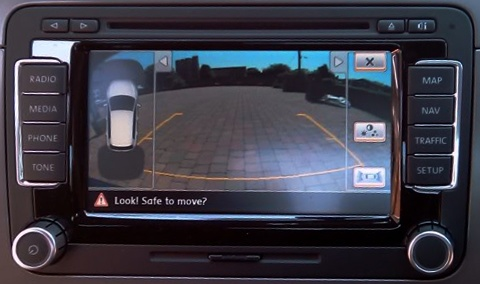
\includegraphics{parking}}\\
     \caption{Optical parking system for a car\label{fig:parking}}
   \end{center}
\end{figure}

The downside of using a compiled language is that a developer is required to make changes to the source code, save them in a file, compile that file to create a binary file, and then re-run that binary file. In contrast, \textbf{interpreted languages} offer considerable savings in development time. In an interpreted language \emph{the developer can enter code and have it run straight away}. \fig{cycle} shows that the feedback cycle in an interpreted language is much shorter than the one of a compiled language. 
\begin{figure}[htbp]
  \begin{center}
    \begin{minipage}[t]{.4\textwidth}
      \begin{center}
        \resizebox{\textwidth}{!}{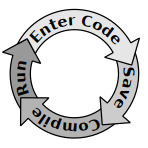
\includegraphics{cycle-static}}\\
        Compiled language
      \end{center}
    \end{minipage}
    \hspace{1cm}
    \begin{minipage}[t]{.4\textwidth}
      \begin{center}
        \resizebox{\textwidth}{!}{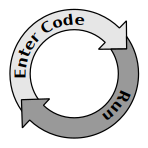
\includegraphics{cycle-dynamic}}\\
        Interpreted language
      \end{center}
    \end{minipage}
    \caption{Feedback cycle in a compiled and in an interpreted language\label{fig:cycle}}
  \end{center}
\end{figure}

A shorter feedback cycle consumes less time as the developer does not need to spend time waiting for the result of the previous change. The immediate feedback also fits well with the human learning process. Immediate feedback about the progress being made is a requirement for the human mind to enter a state of ``flow'' where it operates at full capacity~\citep{nakamura2002concept,lister1987peopleware}.

Even though interpreted languages have been applied to machine vision as early as \citeyear{mundy} (see \citet{mundy}), machine vision systems are still predominantly implemented using compiled languages.
%\begin{figure}[htbp]
%   \begin{center}
%     \resizebox{.6\textwidth}{!}{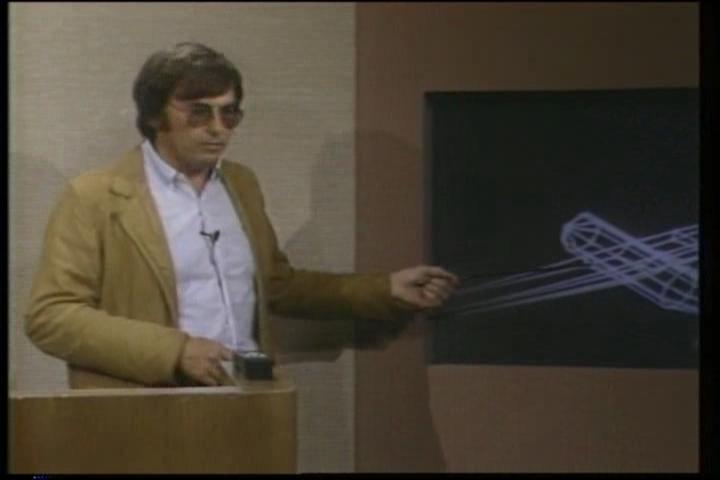
\includegraphics{mundy}}\\
%     \caption{Joseph Mundy presenting a machine vision system implemented in LISP\label{fig:mundy}}
%   \end{center}
%\end{figure}
The reason is that if an embedded system is produced in large quantities, it is possible to offset the considerable software development cost against small per-unit savings in hardware cost. However this trade-off might become less important with the advent of modern embedded hardware (\fig{arm} for example shows the Gumstix board which is an embedded computer capable of running an operating system).
\begin{figure}[htbp]
   \begin{center}
     \resizebox{.6\textwidth}{!}{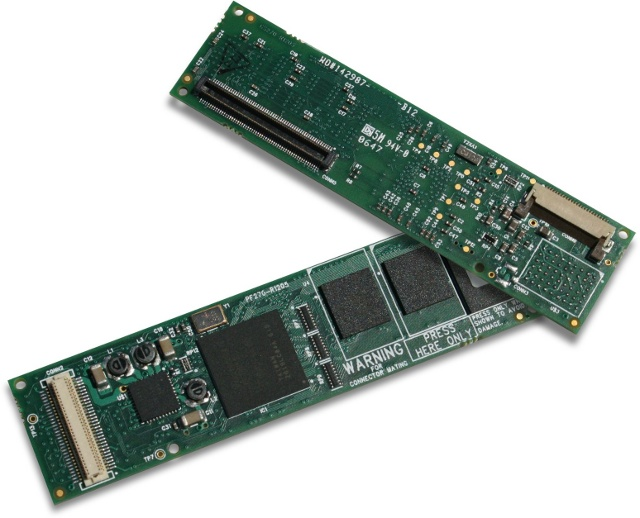
\includegraphics{gumstix}}\\
     \caption{ARM Gumstix boards\label{fig:arm}}
   \end{center}
\end{figure}

It can be argued that the widespread adoption of compiled languages is currently hampering innovation~\citep{RefWorks:311}. The publication by \citet{RefWorks:480} demonstrates that robotic projects can greatly benefit from the properties of the interpreted programming language Ruby. Interpreted languages not only allow for concise code, they also make interactive manipulation of data possible where one can confirm the results immediately.

\section{Dynamically Typed Languages}\label{cha:dyntyped}
% define static typing, dynamic typing, history? <-> hardware
The benefits of using an interpreted language are quite obvious. A less visible but nevertheless important issue is the difference between \emph{statically typed languages} and \emph{dynamically typed languages}. Note that this issue should not be confused with the issue of strong typing versus weak typing. A language is statically typed if all type checks are performed at compile-time. Dynamically typed languages on the other hand perform type checks at run-time and allow to define new types at run-time. Dynamic typing however makes early method binding impossible which has a negative impact on run-time performance. \fig{binding} gives an example. In C++ the \code{+} operation can be compiled to a machine instruction (\eg \code{ADD AX, 1}). The method \code{test} is limited to processing integers. In Ruby however it is in general impossible to determine whether the value of \code{x} always will be an integer. \Eg the value might be a floating point number or a rational number.
\begin{figure}[htbp]
  \begin{center}
    \begin{minipage}[b]{.4\textwidth}
      \begin{center}
        \lstset{language=C++,frame=single,numbers=none}
        \begin{lstlisting}
int test(int x)
{
  return x + 1;
}
// ...
  int y = test(42);
// ...
        \end{lstlisting}
        C++ (early method binding)
      \end{center}
    \end{minipage}\hspace{3ex}
    \begin{minipage}[b]{.4\textwidth}
      \begin{center}
        \lstset{language=Ruby,frame=single,numbers=none}
        \begin{lstlisting}
def test(x)
  x + 1
end
# ...
y = test 42
z = test Complex::I
        \end{lstlisting}
        Ruby (late method binding)
      \end{center}
    \end{minipage}
  \end{center}
  \caption{Early vs. late method binding\label{fig:binding}}
\end{figure}

Type safety is a term to describe the fact that static typing prevents certain programming errors such as type mismatches or misspelled method names from entering production code. With static typing it is possible to reject these kind of errors at compile time. Statically typed languages are engrained in safety critical systems such as nuclear power plants, air planes, and industrial robots because of increased type safety. \fig{typing} gives an example where the bug in the C++ program is rejected by the compiler. The equivalent Ruby program however discovers the error only at run-time and only for certain input.
\begin{figure}[htbp]
  \begin{center}
    \begin{minipage}[b]{.5\textwidth}
      \begin{center}
        \lstset{language=C++,frame=single,numbers=none}
        \begin{lstlisting}
#include <stdlib.h>
int main(int argc, char *argv[])
{
  int x = atoi(argv[1]);
  if (x == 0) x += "test";
  // error: invalid conversion from
  //   'const char*' to 'int'
  return 0;
}
        \end{lstlisting}
        C++ (static typing)
      \end{center}
    \end{minipage}\hspace{3ex}
    \begin{minipage}[b]{.3\textwidth}
      \begin{center}
        \lstset{language=Ruby,frame=single,numbers=none}
        \begin{lstlisting}
x = ARGV[0].to_i
x += "test" if x == 0
        \end{lstlisting}
        Ruby (dynamic typing)
      \end{center}
    \end{minipage}
  \end{center}
  \caption{Static typing vs. dynamic typing. \ccout\label{fig:typing}}
\end{figure}

However statically typed implementations tend to become inflexible. \Ie when a developer wants to modify one aspect of the system, the static typing can force numerous rewrites in unrelated parts of the source code~\citep{RefWorks:486}. Development and maintenance of large scale systems using a statically typed language is much more expensive compared to when using a dynamically typed languages~\citep{RefWorks:311}. Heavy users of statically typed languages tend to introduce custom mechanisms to deal with the absence of support for reflection and meta-programming in their language (see the CERN's C++ framework for example \cite{Antcheva20092499}).

Though offering some safety, static typing does not prevent programming errors such as numerical overflow or buffer overflow~\citep{RefWorks:486}. \Ie the efficiency gained by using C or C++ is at the cost of security~\citep{wolczko}. \fig{staticnumber} shows two programs where numerical overflow occurs if a native integer type of insufficient size is chosen.
\begin{figure}[htbp]
  \lstset{language=C++,frame=single,numbers=none}
  \begin{center}
    \begin{minipage}[c]{.4\textwidth}
      \begin{center}
        \begin{lstlisting}
#include <iostream>
using namespace std;
int main(void)
{
  int x = 2147483648;
  x += 1;
  cout << x << endl;
  // -2147483647
  return 0;
}
        \end{lstlisting}
        32-bit integer
      \end{center}
    \end{minipage}\hspace{3ex}
    \begin{minipage}[c]{.4\textwidth}
      \begin{center}
        \begin{lstlisting}
#include <iostream>
using namespace std;
int main(void)
{
  long x = 2147483648;
  x += 1;
  cout << x << endl;
  // 2147483649
  return 0;
}
        \end{lstlisting}
        64-bit integer
      \end{center}
    \end{minipage}
  \end{center}
  \caption{Static typing and numeric overflow. \cout\label{fig:staticnumber}}
\end{figure}
A well known example is the failure of the first Ariane 5 (shown in \fig{ariane}) due to an arithmetic overflow (see talk by \citealp{fenwick2008}).
\begin{figure}[htbp]
   \begin{center}
     \resizebox{.6\textwidth}{!}{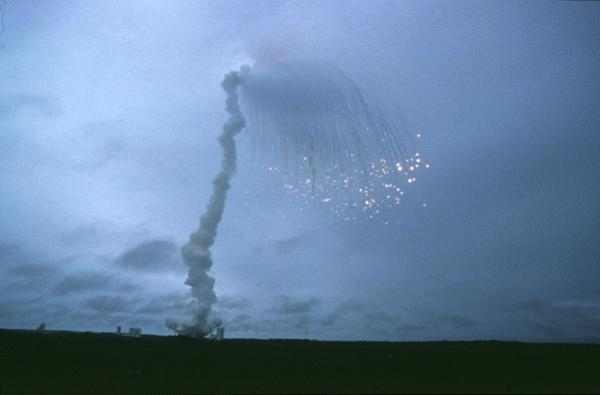
\includegraphics{ariane5}}\\
     \caption{Ariane 5 disaster caused by numerical overflow\label{fig:ariane}}
   \end{center}
\end{figure}
\Ie even when using static typing, it is still necessary to use techniques such as software assertions or unit tests to prevent runtime errors from happening.

Dynamic typing on the other hand allows to combine integers, rational numbers, complex numbers, vectors, and matrices in a seamless way. The Ruby core library makes use of dynamic typing to represent integers, big numbers, floating point numbers, complex numbers, and vectors work together seamlessly (see \sct{dynnum} for more details).

Ruby data types do not map well to native data types (\ie the integer and floating-point registers of the hardware). \Eg Ruby integers do not exhibit numerical overflow and the boundaries of Ruby arrays are resized dynamically. Furthermore dynamic typing requires late binding of method calls which is computationally expensive on current hardware~\citep{RefWorks:484}. This thesis tries to address these problems by defining representations of native types in a Ruby extension\footnote{Ruby libraries are generally called ``Ruby extensions''} (see \sct{contrib}).

\section{Contributions of this Thesis}\label{cha:contrib}
The title of this thesis is ``\xtitle'', The Ruby extension implemented in the context of this thesis makes it possible for researchers and developers working in the field of image processing and computer vision to take advantage of the benefits offered by this dynamically typed language. The phrase ``efficient implementation'' was intentionally used in an ambiguous way. It can mean
\begin{itemize}
\item \textbf{machine efficiency}: The run-time performance of the system is sufficient to implement real-time machine vision systems.
\item \textbf{developer efficiency}: The programming language facilitates concise and flexible implementations which means that developers can achieve high productivity.
\end{itemize}

The contribution of this thesis is a \added{set of} computer vision extension\added{s} for the existing Ruby programming language. The extension\added{s} \emph{bring\removed{s} together performance and \changed{flexibility}{productivity} in an unprecedented way}. \added{The Ruby extensions provide}
\begin{itemize}
\item \added{extensive \ac{I}/\ac{O} integration for image- and video-data}
\item \added{generic array operations for uniform multi-dimensional arrays}
  \begin{itemize}
  \item \added{a set of objects to represent arrays, array views, and lazy evaluations in a modular fashion}
  \item \added{optimal type coercions for all combinations of operations and data types}
  \end{itemize}
\end{itemize}

\changed{It supports}{The work presented in this thesis brings together} several concepts which previously have not been integrated in a single computer vision system:
\begin{itemize}
\item \emph{expressiveness:} An \changed{internal DSL}{library} for manipulating uniform arrays is introduced. A generic set of basic operations is used to build computer vision algorithms from the ground up.
\item \emph{lazy evaluation:} Lazy evaluation of array operations makes it possible to reduce memory-\acs{I}/\acs{O}. \added{This facilitates the use of \ac{GPGPU} (not done as part of this thesis) where memory-\acs{I}/\acs{O} is the performance-bottleneck.}
\item \emph{array views:} Shared references make it possible to extract sub-arrays without making a ``deep copy'' of the array.
\item \emph{transparent \ac{JIT} compilation:} A \ac{JIT} compiler and a cache are integrated transparently to achieve real-time performance.
\item \emph{\ac{I}/\ac{O} integration:} The implementation also provides integration for image- and video-\acs{I}/\acs{O} (see \fig{architecture}) as well as the necessary colour space conversions.
\end{itemize}
\begin{figure}[htbp]
   \begin{center}
     \resizebox{.8\textwidth}{!}{\includegraphics{architecture}}\\
     \caption{Software architecture of machine vision system\label{fig:architecture}}
   \end{center}
\end{figure}
\added{The functionality was implemented in a modular way (see \sct{arrays}). The result is a com\-pre\-hen\-si\-ve approach to implementing computer vision algorithms.}
% expand contribution of this thesis, include issue of fast prototyping for Ruby !!!

The type system and the expressions presented in \cha{rubyvision} constitute the \changed{DSL}{library} which was developed as part of this thesis. If some of the expressions appear to be part of the Ruby syntax at first sight, it is due to the dynamic nature of the programming language. Although the Ruby programming language was used, this approach could be applied to other dynamically typed languages with sufficient meta-programming support. The approach presented in this thesis could also be used to provide transparent integration of \acp{GPU} for parallel processing. Finally the facilitation of succinct implementations of various computer vision algorithms allows for a more formal understanding of computer vision.

\section{Thesis Outline}\label{cha:outline}
\cha{intro} (this chapter) showed that there is sufficient motivation to address the performance issues involved with applying a dynamically typed language to the problem of implementing machine vision algorithms. Apart from offering productivity gains, dynamically typed languages also make it possible to combine various types and operations seamlessly.

\cha{state} gives an overview of the state of the art in machine vision software, illustrating the difficulty of achieving performance and \changed{flexibility}{productivity} at the same time. It will be shown that the performance of the Ruby \ac{VM} is significantly lower than the performance achieved with \acs{GNU} C. But it will also be argued that \ac{AOT} compilation is incompatible with the goal of achieving \changed{flexibility}{productivity}.

\cha{rubyvision} is about the core of the work presented in this thesis. Starting with memory objects and native data types, a \changed{DSL}{library} for describing computer vision algorithms is introduced. It is demonstrated how this approach facilitate succinct implementations of basic image processing operations. \ac{JIT} compilation is used to address the issue of performance.

\cha{io} covers key issues in implementing interfaces for \acl{I} and \acl{O} of image data. Image \ac{I}/\ac{O} involving cameras, image files, video files, and video displays is discussed. The key issues are colour space compression, image and video compression, \ac{LDR} versus \ac{HDR} imaging, and \ac{GUI} integration.

In \cha{vision} it is shown how different algorithms which are common in the field of computer vision can be implemented using the concepts introduced in chapter \cha{rubyvision} and \cha{io}.

\cha{results} shows some examples of complete applications implemented using the Hornetseye Ruby extension which was developed as part of this thesis \added{(see page \pageref{cha:software})}. Furthermore a performance comparison is given.

At the end of the thesis \cha{future} offers conclusions and future work.

\begin{savequote}[8cm]
  \begin{singlespace}
    ``There are two ways of constructing a software design: One way is to make it so simple that there are obviously no deficiencies, and the other way is to make it so complicated that there are no obvious deficiencies. The first method is far more difficult.''
    \qauthor{Sir Charles Antony Richard Hoare}
    ``I am a historian and a computer programmer, but primarily I am a lawyer. My research, ongoing for a decade, follows a purely experimental paradigm:
    \begin{enumerate}
    \item Try to create freedom by destroying illegitimate power sheltered behind intellectual property law.
    \item See what happens.
    \end{enumerate}
    Early results are encouraging.''
    \qauthor{Eben Moglen}
    % ``The reasonable man adapts himself to the world; the unreasonable one persists in trying to adapt the world to himself. Therefore all progress depends on the unreasonable man.''
    % \qauthor{George Bernard Shaw}
  \end{singlespace}
\end{savequote}
\chapter{State of the Art}\label{cha:state}
This chapter gives an overview of the state of the art in machine vision systems, it discusses the features of the Ruby programming language, and available \ac{JIT} compilers are discussed
\begin{itemize}
\item \sct{object} shows the typical structure of an \changed{object recognition}{object localisation} system
\item \sct{foss} gives an overview of \changed{current machine vision systems}{a typical object localisation algorithm} and how \changed{they are}{it is} implemented
\item \sct{ruby} characterises the Ruby programming language by describing the paradigms it supports
\item \sct{jits} points out different \ac{JIT} compilers and their properties
\item \sct{sumstate} gives a summary of this chapter
\end{itemize}

\section{Object Localisation}\label{cha:object}
The task of an object \changed{recognition}{localisation} algorithm is to determine the pose of known objects given a camera image as input. \fig{overview} shows an overview of a typical object \changed{recognition}{localisation} algorithm. The processing steps are explained in \tbl{steps}.
\begin{figure}[htbp]
   \begin{center}
     \resizebox{\textwidth}{!}{
\includegraphics{overview}}\\
     \caption{Overview of a typical object localisation algorithm\label{fig:overview}}
   \end{center}
\end{figure}
\begin{table}[htbp]
  \begin{center}
    \caption{Processing steps performed by a typical machine vision
      systems\label{tbl:steps}}\vspace{1em}
    \begin{tabular}{ll}\toprule
      \textbf{Processing step} & \textbf{Details} \\\midrule
      \emph{preprocessing}              & \parbox[t]{.6\textwidth}{basic operations such as filtering, thresholding, morphology and the like are applied to the image}\\
      \emph{key-point localisation} & \parbox[t]{.6\textwidth}{a feature extraction method defines feature locations in the image}\\
      \emph{feature description}     & \parbox[t]{.6\textwidth}{the descriptors for the local feature context are computed}\\
      \emph{recognition/tracking}    & \parbox[t]{.6\textwidth}{the features are used to recognise and track known objects in the scene}\\\bottomrule
    \end{tabular}
  \end{center}
\end{table}
The processing steps are not mandatory. Some algorithms do not use feature descriptors (\eg Geometric Hashing~\citep{RefWorks:22}). Some algorithms for \ac{2D} object \changed{recognition}{localisation} do not even use features at all (\eg Fast Normalised Cross-Correlation~\citep{lewis1995fast}).

Current \ac{3D} object recognition and tracking algorithms however are predominantly based on feature extraction and feature matching (\eg spin image features by \citet{RefWorks:91}, Geometric Hashing~\citep{RefWorks:22}, Bounded Hough Transform~\citep{RefWorks:36}, \ac{RANSAC} \citep{RefWorks:84}). Approaches based on feature matching are furthermore used to deal with related problems such as real-time \ac{SLAM} \citep[\eg][]{RefWorks:569,RefWorks:513} and \ac{3D} modelling \citep[\eg][]{pan2009ProFORMA,RefWorks:499,RefWorks:354,RefWorks:500}.

There are more unconventional techniques (\eg tensor factorisation~\citep{RefWorks:564}, integral images~\citep{Viola01robustreal-time}) but they are mostly applied to object detection. \Ie the algorithms detect the presence of an object but do not estimate its pose.

\section{Existing \acs{FOSS} for Machine Vision}\label{cha:foss}
A survey of existing \ac{FOSS} for machine vision has been conducted in order to find out about commonalities of current algorithms in use and how current computer vision systems are implemented.

\begin{table}[htbp]
  \begin{center}
    \caption{Existing \acs{FOSS} libraries for Machine Vision I/II\label{tbl:foss1}}\vspace{1em}
    \begin{tabular}{l|ccccccccc}\toprule
      \textbf{feature} &
      \begin{sideways}\href{http://www.ces.clemson.edu/~stb/blepo/}{\textbf{Blepo}}\end{sideways} &
      \begin{sideways}\href{http://camellia.sourceforge.net/}{\textbf{Camellia}}\end{sideways} &
      \begin{sideways}\href{http://www.cs.cmu.edu/~jbruce/cmvision/}{\textbf{CMVision}}\end{sideways} &
      \begin{sideways}\href{http://mi.eng.cam.ac.uk/~er258/cvd/}{\textbf{libCVD}}\end{sideways} &
      \begin{sideways}\href{http://www.easyvision.googlepages.com/}{\textbf{EasyVision}}\end{sideways} &
      \begin{sideways}\href{http://filters.sourceforge.net/}{\textbf{Filters}}\end{sideways} &
      \begin{sideways}\href{http://framewave.sourceforge.net/}{\textbf{Framewave}}\end{sideways} &
      \begin{sideways}\href{http://gamera.informatik.hsnr.de/}{\textbf{Gamera}}\end{sideways} &
      \begin{sideways}\href{http://gandalf-library.sourceforge.net/}{\textbf{Gandalf}}\end{sideways}\\\midrule
      Camera Input         & \tick & \xxxx & \tick & \tick & \tick & \xxxx & \xxxx & \xxxx & \xxxx \\
      Image Files          & \tick & \tick & \xxxx & \tick & \tick & \tick & \tick & \tick & \tick \\
      Video Files          & \xxxx & \xxxx & \xxxx & \tick & \xxxx & \xxxx & \tick & \xxxx & \xxxx \\
      Display              & \tick & \xxxx & \tick & \tick & \tick & \xxxx & \xxxx & \tick & \tick \\
      Scripting            & \xxxx & \tick & \xxxx & \xxxx & \tick & \xxxx & \xxxx & \tick & \xxxx \\
      Warps                & \xxxx & \xxxx & \xxxx & \tick & \xxxx & \xxxx & \tick & \xxxx & \tick \\
      Histograms           & \xxxx & \xxxx & \tick & \xxxx & \xxxx & \tick & \xxxx & \tick & \tick \\
      Custom Filters       & \tick & \xxxx & \xxxx & \tick & \xxxx & \tick & \tick & \tick & \tick \\
      Fourier Transforms   & \tick & \xxxx & \xxxx & \xxxx & \xxxx & \xxxx & \xxxx & \xxxx & \tick \\
      Feature Extraction   & \tick & \xxxx & \xxxx & \tick & \tick & \tick & \tick & \tick & \tick \\
      Feature Matching     & \tick & \xxxx & \xxxx & \xxxx & \tick & \xxxx & \xxxx & \xxxx & \xxxx \\
      \acs{GPL} compatible & \tick & \tick & \tick & \tick & \qqqq & \tick & \tick & \tick & \tick \\\bottomrule
    \end{tabular}
  \end{center}
\end{table}
\begin{table}[htbp]
  \begin{center}
    \caption{Existing \acs{FOSS} libraries for Machine Vision II/II\label{tbl:foss2}}\vspace{1em}
    \begin{tabular}{l|ccccccccc}\toprule
      \textbf{feature} &
      \begin{sideways}\href{http://www.itk.org/Insight/Doxygen/html/index.html}{\textbf{ITK/VTK}}\end{sideways} &
      \begin{sideways}\href{http://ivt.sourceforge.net/}{\textbf{IVT}}\end{sideways} &
      \begin{sideways}\href{http://ltilib.sourceforge.net/doc/homepage/index.shtml}{\textbf{LTIlib}}\end{sideways} &
      \begin{sideways}\href{http://lush.sourceforge.net/}{\textbf{Lush}}\end{sideways} &
      \begin{sideways}\href{http://vision.eng.shu.ac.uk/mediawiki/index.php/Mimas}{\textbf{Mimas}}\end{sideways} &
      \begin{sideways}\href{http://ti.arc.nasa.gov/projects/visionworkbench/}{\textbf{NASA V. W.}}\end{sideways} &
      \begin{sideways}\href{http://opencv.willowgarage.com/}{\textbf{OpenCV}}\end{sideways} &
      \begin{sideways}\href{http://www.doc.ic.ac.uk/~ajd/software.html}{\textbf{SceneLib}}\end{sideways} &
      \begin{sideways}\href{http://kogs-www.informatik.uni-hamburg.de/~koethe/vigra/}{\textbf{VIGRA}}\end{sideways}\\\midrule
      Camera Input         & \xxxx & \tick & \tick & \tick & \tick & \xxxx & \tick & \tick & \xxxx \\
      Image Files          & \tick & \tick & \tick & \tick & \tick & \tick & \tick & \xxxx & \tick \\
      Video Files          & \xxxx & \tick & \xxxx & \xxxx & \tick & \xxxx & \tick & \xxxx & \xxxx \\
      Display              & \tick & \tick & \tick & \tick & \tick & \xxxx & \tick & \tick & \xxxx \\
      Scripting            & \xxxx & \xxxx & \xxxx & \tick & \xxxx & \xxxx & \tick & \xxxx & \xxxx \\
      Warps                & \tick & \xxxx & \xxxx & \tick & \tick & \tick & \tick & \xxxx & \xxxx \\
      Histograms           & \tick & \tick & \tick & \tick & \xxxx & \xxxx & \tick & \xxxx & \xxxx \\
      Custom Filters       & \tick & \tick & \tick & \tick & \tick & \tick & \xxxx & \xxxx & \tick \\
      Fourier Transforms   & \tick & \xxxx & \xxxx & \xxxx & \tick & \xxxx & \tick & \xxxx & \tick \\
      Feature Extraction   & \tick & \tick & \tick & \tick & \tick & \xxxx & \tick & \tick & \tick \\
      Feature Matching     & \xxxx & \tick & \tick & \xxxx & \xxxx & \xxxx & \tick & \tick & \xxxx \\
      \acs{GPL} compatible & \tick & \tick & \tick & \tick & \tick & \xxxx & \tick & \tick & \tick \\\bottomrule
    \end{tabular}
  \end{center}
\end{table}
\tbl{foss1} and \tbl{foss2} give an overview of noticeable computer vision libraries. The libraries where checked against a set of features. Each check mark signifies a feature being supported by a particular library. One can see that no library completely covers all the features which are typically required to develop an object recognition and tracking system as shown in \fig{overview}.

One can distinguish three different kinds of libraries: statically typed libraries, statically typed extensions for a dynamically typed language, and dynamically typed libraries.

\subsection{Statically Typed Libraries}\label{cha:statically}
Most computer vision libraries are implemented in the statically typed C/C++ language. However C++ has a split type system. There are primitive types which directly correspond to registers of the hardware and there are class types which support inheritance and dynamic dispatch. In C++ not only integers and floating point numbers but also arrays are primitive types. However these are the most relevant data types for image processing. To implement a basic operation such as adding two values so that it will work on different types, one needs to make extensive use of template meta-programming. \Ie all combinations of operations, element-type(s), and number of dimensions have to be instantiated separately. For example the FrameWave\footnote{\url{http://framewave.sourceforge.net/}} C-library has 42 explicitly instantiated different methods for multiplying arrays.

For this reason most libraries do not support all possible combinations of element-types and operations. Assume a library supports the following 10 binary operations
\begin{itemize}
\item addition (\code{+})
\item subtraction (\code{-})
\item division (\code{/})
\item multiplication (\code{*})
\item exponent (\code{**})
\item greater or equal (\code{$>=$})
\item \changed{less}{greater} than (\code{$>$})
\item less or equal (\code{$<=$})
\item less than (\code{$<$})
\item equal to (\code{$==$})
\end{itemize}
Furthermore assume that it supports the following types as scalars and array elements
\begin{itemize}
\item 6 integer types: 8-,16-, and 32-bit, signed/unsigned
\item 2 floating-point types: single/double precision
\end{itemize}
Finally for every binary operation there are the following variations
\begin{itemize}
\item scalar-array operation
\item array-scalar operation
\item array-array operation
\end{itemize}
This results in $10\cdot 8\cdot 8\cdot 3=1920$ possible combinations of operations and element-types. \Ie to fully support the 10 binary operations on these element-types requires $1920$ methods to be defined either directly or by means of C++ template programming. \Ie static typing and ahead-of-time compilation leads to a explosion of combinations of basic types and operations. \lst{cop} shows how much code is required when using C++ templates to implement a element-wise \code{+} operator (array-array operation only) for the \code{boost::multi\_array} data types provided by the Boost library. The implementation works on arrays of arbitrary dimension and arbitrary element-type.

\lstset{language=C++,frame=single,numbers=none}
\begin{lstlisting}[float=htbp,caption={Multi-dimensional ``+'' operator implemented in C++. \cout},label=lst:cop]
#include <boost/multi_array.hpp> // 3726 lines of code
#include <iostream>
using namespace boost;
template< typename T >
T &multi_plus(T &a, const T &b, const T &c) {
  a = b + c;
  return a;
}
template< template< typename, size_t, typename > class Arr, typename Alloc,
          typename T, size_t N >
detail::multi_array::sub_array< T, N > multi_plus
  (detail::multi_array::sub_array< T, N > a, const Arr< T, N, Alloc > &b,
   const Arr< T, N, Alloc > &c) {
  typename Arr< T, N, Alloc >::const_iterator j = b.begin(), k = c.begin();
  for (typename detail::multi_array::sub_array< T, N >::iterator i =
       a.begin(); i != a.end(); i++, j++, k++)
    multi_plus(*i, *j, *k);
  return a;
}
template< template< typename, size_t, typename > class Arr, typename Alloc,
          typename T, size_t N >
Arr< T, N, Alloc > &multi_plus
  (Arr< T, N, Alloc > &a, const Arr< T, N, Alloc > &b,
   const Arr< T, N, Alloc > &c) {
  typename Arr< T, N, Alloc >::const_iterator j = b.begin(), k = c.begin();
  for (typename Arr< T, N, Alloc >::iterator i = a.begin();
       i != a.end(); i++, j++, k++)
    multi_plus(*i, *j, *k);
  return a;
}
template < template< typename, size_t, typename > class Arr, typename Alloc,
           typename T, size_t N >
multi_array< T, N > operator+
  (const Arr< T, N, Alloc > &a, const Arr< T, N, Alloc > &b) {
  array< size_t, N > shape;
  std::copy(a.shape(), a.shape() + N, shape.begin());
  multi_array< T, N > retVal(shape);
  multi_plus(retVal, a, b);
  return retVal;
};
int main(void) {
  multi_array< int, 2 > a(extents[2][2]);
  a[0][0] = 1; a[0][1] = 2; a[1][0] = 3; a[1][1] = 4;
  multi_array< int, 2 > b(extents[2][2]);
  b[0][0] = 5; b[0][1] = 4; b[1][0] = 3; b[1][1] = 2;
  multi_array< int, 2 > r(a + b);
  std::cout << "[[" << r[0][0] << ", " << r[0][1] << "], ["
            << r[1][0] << ", " << r[1][1] << "]]" << std::endl;
  // [[6, 6], [6, 6]]
  return 0;
}
\end{lstlisting}

Static typing not only leads to an explosion of methods to instanciate. A related problem caused by static typing is that when a developer wants to modify one aspect of the system, the static typing can force numerous rewrites in unrelated parts of the source code~\citep{RefWorks:486}. Static typing enforces unnecessary ``connascence'' (a technical term introduced by \citet{weirich2009}, also see \anx{connascence}) which interferes with the modularity of the software.
In practise this causes problems when implementing operations involving scalars, complex numbers, and \acs{RGB}-triplets~\citep{RefWorks:560}. \fig{ops} shows that binary operations are not defined for some combinations of the argument types involved.
\begin{figure}[htbp]
  \begin{center}
    \resizebox{.65\textwidth}{!}{
      \begin{picture}(0,0)
        \input{operatortable.pstex_t}
      \end{picture}
      \includegraphics{operatortable}}\caption{Binary operations for
      different element types~\citep{RefWorks:560}\label{fig:ops}}
  \end{center}
\end{figure}
\Ie it is not sufficient to simply use C++ templates to instantiate all combinations of operations and argument types. One also has to address the problem that binary operations usually only are meaningful only for some combinations of element-types.

Finally using a combination of multiple libraries is hard, because each library usually comes with its own set of data types for representing images, arrays, matrices, and other elements of signal processing.

\subsection{Statically Typed Extensions}\label{cha:staticext}
Some computer vision libraries come with bindings in order to use them as an extension to a dynamically typed language. \Eg for the OpenCV\footnote{\url{http://opencv.willowgarage.com/}} library there are Python bindings (PyCV\footnote{\url{http://pycv.sharkdolphin.com/}}) as well as Ruby bindings (opencv.gem\footnote{\url{http://rubyforge.org/projects/opencv/}}). Some projects (\eg the Gamera \ac{OCR} software \citep{Droettboom03thegamera} and the Camellia\footnote{\url{http://camellia.sourceforge.net}} Ruby extension) use the Simplified Wrapper Generator (SWIG\footnote{\url{http://swig.org/}}) to generate bindings from C/C++ header files. This allows one to use a statically typed extension in an interpreted language and it becomes possible to develop machine vision software interactively without sacrificing performance.

Open classes and dynamic typing make it possible to seamlessly integrate the functionality of one library into the \ac{API} of another. \Eg \lst{rmagick} shows how one can extend the NArray\footnote{\url{http://narray.rubyforge.org/}} class to use the RMagick\footnote{\url{http://rmagick.rubyforge.org/}} library for loading images. The method \code{NArray\#read} reads an image using the RMagick extension. The image is exported to a Ruby string which in turn is imported into an object of type \code{NArray}. The image used in this example is shown in \fig{circle}.
\begin{figure}[htbp]
  \begin{center}
    \framebox{\resizebox{.2\textwidth}{!}{
\includegraphics{circle}}}
    \caption{Low resolution image of a circle\label{fig:circle}}
  \end{center}
\end{figure}
\lstset{language=Ruby,frame=single,numbers=none}
\begin{lstlisting}[float=htbp,caption={Integrating RMagick and NArray in Ruby. \rubyout},label=lst:rmagick]
require 'narray'
require 'RMagick'
class NArray
  def NArray.read(filename)
    img = Magick::Image.read(filename)[0]
    str = img.export_pixels_to_str 0, 0, img.columns, img.rows, "I",
          Magick::CharPixel
    to_na str, NArray::BYTE, img.columns, img.rows
  end
end
arr = NArray.read 'circle.png'
arr / 128
# NArray.byte(20,20):
# [ [ 1, 1, 1, 1, 1, 1, 1, 0, 0, 0, 0, 0, 0, 1, 1, 1, 1, 1, 1, 1 ],
#   [ 1, 1, 1, 1, 1, 0, 0, 0, 0, 0, 0, 0, 0, 0, 0, 1, 1, 1, 1, 1 ],
#   [ 1, 1, 1, 0, 0, 0, 0, 0, 0, 0, 0, 0, 0, 0, 0, 0, 0, 1, 1, 1 ],
#   [ 1, 1, 0, 0, 0, 0, 0, 0, 0, 0, 0, 0, 0, 0, 0, 0, 0, 0, 1, 1 ],
#   [ 1, 1, 0, 0, 0, 0, 0, 0, 0, 0, 0, 0, 0, 0, 0, 0, 0, 0, 1, 1 ],
#   [ 1, 0, 0, 0, 0, 0, 0, 0, 0, 0, 0, 0, 0, 0, 0, 0, 0, 0, 0, 1 ],
#   [ 1, 0, 0, 0, 0, 0, 0, 0, 0, 0, 0, 0, 0, 0, 0, 0, 0, 0, 0, 1 ],
#   [ 0, 0, 0, 0, 0, 0, 0, 0, 0, 0, 0, 0, 0, 0, 0, 0, 0, 0, 0, 0 ],
#   [ 0, 0, 0, 0, 0, 0, 0, 0, 0, 0, 0, 0, 0, 0, 0, 0, 0, 0, 0, 0 ],
#  ...
\end{lstlisting}

However supporting all possible combinations of types and operations with a statically typed library is hard (see \sct{statically}). In practise most computer vision extensions only provide a subset of all combinations. \lst{cvmat} shows that the OpenCV library for example supports element-wise addition of \ac{2D} arrays of 8-bit unsigned integers (line 3).
\lstset{language=Ruby,frame=single,numbers=left}
\begin{lstlisting}[float=htbp,caption={Using OpenCV in Ruby. \rubyout},label=lst:cvmat]
require 'opencv'
include OpenCV
CvMat.new(6, 2, CV_8U) + CvMat.new(6, 2, CV_8U)
# <OpenCV::CvMat:2x6,depth=cv8u,channel=3>
CvMat.new(6, 2, CV_8U) + CvMat.new(6, 2, CV_16U)
#(irb):4: warning: OpenCV error code (-205) : cvAdd (840 in cxarithm.cpp)
#OpenCV::CvStatusUnmatchedFormats: 
#        from (irb):4:in `+'
#        from (irb):4
\end{lstlisting}
But trying to add elements of 8-bit unsigned and 16-bit unsigned will cause an exception (line 5). Other libraries such as EasyVision\footnote{\url{http://perception.inf.um.es/easyVision/}} (an extension for Haskell) even have different method names depending on the types of arguments involved. \Eg \code{absDiff8u} to compute the element-wise absolute difference of arrays of 8-bit unsigned integers or \code{sqrt32f} to compute the element-wise square root of arrays of 32-bit floating point values.

In contrast to the previously mentioned libraries, the NArray\footnote{\url{http://narray.rubyforge.org/}}~\citep{narray1,narray2} Ruby extension supports adding arrays with different element-types (see \lst{narray}).
\lstset{language=Ruby,frame=single,numbers=none}
\begin{lstlisting}[float=htbp,caption={Using NArray in Ruby. \rubyout},label=lst:narray]
require 'narray'
a = NArray.byte 6, 2
# NArray.byte(6,2): 
# [ [ 0, 0, 0, 0, 0, 0 ], 
#   [ 0, 0, 0, 0, 0, 0 ] ]
b = NArray.sint 6, 2
# NArray.sint(6,2): 
# [ [ 0, 0, 0, 0, 0, 0 ], 
#   [ 0, 0, 0, 0, 0, 0 ] ]
a + b
# NArray.sint(6,2): 
# [ [ 0, 0, 0, 0, 0, 0 ], 
#   [ 0, 0, 0, 0, 0, 0 ] ]
2 * a + b
# NArray.sint(6,2): 
# [ [ 0, 0, 0, 0, 0, 0 ], 
#   [ 0, 0, 0, 0, 0, 0 ] ]
\end{lstlisting}
The library also does optimal return type coercions. \Eg adding an array with single precision complex numbers (\code{NArray::SCOMPLEX}) and an array with double precision floating point numbers (\code{NArray::DFLOAT}) will result in an array of double precision complex numbers (\code{NArray::DCOMPLEX}). In contrast to OpenCV however, the NArray library does not support unsigned integers.

A similar but more sophisticated library is NumPy\footnote{\url{http://numpy.scipy.org/}} for Python \citep[also see][]{Oliphant2006}. NumPy also offers a C-\acs{API} which makes it possible to define custom element-types. \lst{numpy} shows that NumPy supports unsigned integer as well as signed integer types. 
\lstset{language=Python,frame=single,numbers=left}
\begin{lstlisting}[float,caption={Array operations in Python using NumPy. \pythonout},label=lst:numpy]
from numpy import *
a = array([[1, 2], [3, 4]], dtype = int8)
b = array([[1, 2], [3, 4]], dtype = uint16)
a + b
# array([[2, 4],
#        [6, 8]], dtype=int32)
2 * a + b
# array([[3,  6],
#        [9, 12]], dtype=int32)
\end{lstlisting}
In contrast to NArray the result of the type coercion is an array of 32-bit integers (line 4). Similar to the NArray library, NumPy is implemented in C and uses tables of function pointers to do operations on combinations of elements.

The problem with this approach is that the last operation shown in \lst{narray} as well as \lst{numpy} (multiplying an array with two and adding another array) creates an array as intermediate result. \Ie the result of the scalar-array multiplication is written to memory and then read back again when the array-array addition is performed. Since the array operations are just calls to a static library, there is no means of optimising them. For this reason one cannot really use this array operations in order to build higher-level functions without sacrificing performance!

In general it is not possible to instantiate efficient implementations of all the possible combinations of operations and compile them ahead-of-time. \Eg the FTensor C++ library (see \lst{ftensor} for example) allows one to instantiate various tensor operations using C++ templates~\citep{RefWorks:559}.
\lstset{language=C++,frame=single,numbers=none}
\begin{lstlisting}[float,caption={Tensor operation with the FTensor C++ library},label=lst:ftensor]
Index< 'i', 3 > i;
Index< 'j', 3 > j;
Index< 'k', 3 > k;
Tensor2< double, 3, 3 > r, a, b;
r(i, k) = a(i, j) * b(j, k);
\end{lstlisting}
However the library contains code specific to the dimensions $0,1,\ldots,4$. \Ie the functionality of the library is diminished for dimensions higher than $4$.

\subsection{Dynamically Typed Libraries}\label{cha:dynlib}
\lstset{language=Ruby,frame=single,numbers=none}
\begin{lstlisting}[float=htbp,caption={Multi-dimensional ``+'' operator implemented in Ruby. \rubyout},label=lst:rop]
class Array
  def +(other)
    zip(other).collect { |x,y| x + y }
  end
end
a = [[1, 2], [3, 4]]
b = [[5, 4], [3, 2]]
puts (a + b).inspect
# [[6, 6], [6, 6]]
\end{lstlisting}
\lst{rop} shows an implementation of an element-wise \code{+} operator (array-array operation) for the \code{Array} data type of the Ruby standard library. It is much shorter than the equivalent C++ implementation shown in \lst{cop}. \Ie implementing a computer vision library in Ruby is straightforward but there is a performance issue.

\begin{figure}[htbp]
  \begin{center}
    \lstset{language=C,frame=single,numbers=none}
    \begin{minipage}[c]{.45\textwidth}
      \begin{center}
        \begin{lstlisting}
#include <stdlib.h>
#define SIZE 10000000
int main(void)
{
  int i, *arr = (int *)
    malloc(SIZE * sizeof(int));
  for (i = 0; i < SIZE; i++)
    arr[i] = i;
  free(arr);
  return 0;
}
        \end{lstlisting}
        \begin{bf}
          \begin{tabular}{lr@{.}l@{s}}
            gcc 4.2.4 & 0 & 06
          \end{tabular}
        \end{bf}
      \end{center}
    \end{minipage}\hspace{1ex}
    \lstset{language=Ruby,frame=single,numbers=none}
    \begin{minipage}[c]{.5\textwidth}
      \begin{center}
        \begin{lstlisting}
SIZE = 10000000
arr = (0 ... SIZE).collect { |i| i }
        \end{lstlisting}
        \begin{bf}
          \begin{tabular}{lr@{.}l@{s}}
            ruby 1.8.6 & 76 & 3\\
            ruby 1.9.1 &  1 & 8
          \end{tabular}
        \end{bf}
      \end{center}
    \end{minipage}\medskip\\
    \begin{small}
      Intel\textregistered\ Core\texttrademark2 \acs{CPU} T5600 @ 1.83GHz\\
      Linux 2.6.24-24-generic SMP i686 \acs{GNU}/Linux
    \end{small}
  \end{center}
  \caption{Processing time comparison for creating an index array with \acs{GCC} compiled code vs. with the Ruby \acs{VM}\label{fig:arraybench}}
\end{figure}
\fig{arraybench} shows a performance comparison of \acs{GNU} C compiled code and code interpreted with two different versions of the Ruby \ac{VM}. One can see that in the best case the Ruby example is 30 times slower than the equivalent C++ example.

Ruby arrays can contain elements of arbitrary type. \Eg \lst{rarray} shows the definition of the array of integers \code{a} in line 1. In line 9 however one element of \code{a} is set to a string value.
\lstset{language=Ruby,frame=single,numbers=left}
\begin{lstlisting}[float=htbp,caption={Arrays in Ruby. \rubyout},label=lst:rarray]
a = [[2, 3, 5], [7, 11, 13]]
# [[2, 3, 5], [7, 11, 13]]
a[0]
# [2, 3, 5]
a[0][2]
# 5
a[0][3]
# nil
a[0][2] = 'x'
# "x"
a
# [[2, 3, "x"], [7, 11, 13]]
\end{lstlisting}
Also Ruby arrays support dynamic resizing and they do not suffer from buffer overrun. If the array index is out of bounds, a \code{nil} object is returned (\eg see line 7 of \lst{rarray}). This means that Ruby code involving arrays is difficult to optimise. In general it is not possible to remove the dispatcher code and the boundary checks. \Ie the current implementation of Ruby arrays is not suitable for real-time machine vision.

A noteworthy example of a machine vision library implemented in a dynamically typed language is Lush\footnote{\url{http://lush.sourceforge.net/}} which is based on Common Lisp. The Common Lisp programming language supports multi-dimensional arrays~\citep{graham1994lisp}. Line 8 of \lst{clisp} shows that the array type does not support dynamic resizing which makes it possible to generate more efficient code.
\lstset{language=Lisp,frame=single,numbers=left}
\begin{lstlisting}[float=htbp,caption={Arrays in \acs{GNU} Common Lisp. \lispout},label=lst:clisp]
(setq m (make-array '(2 3) :element-type 'integer
  :initial-contents '((2 3 5)(7 11 13))))
; #2A((2 3 5) (7 11 13))
(aref m 0)
*** - AREF: got 1 subscripts, but #2A((2 3 5) (7 11 13)) has rank 2
(aref m 0 2)
; 5
(aref m 0 3)
*** - AREF: subscripts (0 3) for #2A((2 3 5) (7 11 13)) are out of range
(setf (aref m 0 2) "x")
; "x"
m
; #2A((2 3 "x") (7 11 13))
\end{lstlisting}
However the array type still supports elements of arbitrary type even if an element-type was specified (\eg line 10 of \lst{clisp}). \acs{GNU} Common Lisp doesn't seem to support extracting array slices.

It is possible however to introduce uniform arrays as data types and use just-in-time compilation to generate efficient code at run-time. The Lush language demonstrates this approach (Lush was used to implement \ac{OCR} software for example \citep{726791}). \lst{lush} shows some operations involving \ac{2D} arrays.
\lstset{language=Lisp,frame=single,numbers=left}
\begin{lstlisting}[float=htbp,caption={Lush programming language. \lispout},label=lst:lush]
(setq m [i [2 3 5][7 11 13]])
($*0 m 0)
; [i     2     3     5]
(m 0 2)
; 5
(m 0 3)
*** validate-subscript : invalid subscript : 3
(m 0 2 "x")
*** m : not a number : "x"
m
; [i[i     2     3     5]
;   [i     7    11    13]]
? (+ m 1)
= [d[d   3.0000   4.0000   6.0000]
    [d   8.0000  12.0000  14.0000]]
? (* m m)
= [d[d   4.0000   9.0000  25.0000]
    [d  49.0000 121.0000 169.0000]]
\end{lstlisting}
Lush does not support dynamic resizing (\eg line 6 of \lst{lush}) and it enforces uniform arrays (\eg line 8 of \lst{lush}). Although Lush does just-in-time compilation, it defaults to double-precision floating point numbers (\eg line 13 of \lst{lush}) instead of doing optimal coercions like NArray (\lst{narray}). The problem is that implementing support for coercions of native types requires a substantial amount of work and there is insufficient incentive for a developer to invest the time given the low acceptance of the Lisp programming language in the image processing community.

Furthermore Lush is not a Lisp library but it is a Lisp dialect (\ie it is an independent programming language). \Ie there are potential integration issues when using other software developed in different programming languages. A library for a language with broader adoption such as Lisp, \changed{Scheme}{Racket} (former PLT Scheme developed by \citet{Steele1979}), or Clojure\footnote{\url{http://clojure.org/}} would be more desirable.

\section{Ruby Programming Language}\label{cha:ruby}
Ruby is a multi-paradigm language and it is inspired by Perl, Python, Smalltalk, Eiffel, Ada, and Lisp. Ruby supports the following language features
\begin{itemize}
\item object-oriented, single-dispatch
\item dynamic typing
\item exception handling
\item garbage collection (\ie managed environment)
\item mixins
\item closures
\item continuations
\item introspection
\item meta programming
\item reification
\end{itemize}

The Ruby programming language\footnote{\url{http://www.ruby-lang.org/}} was designed by Yukihiro Matsumoto \citetext{see article by \citealp{informit} for a short introduction to Ruby; see \citealp{RefWorks:541}, \citealp{RefWorks:580}, or \citealp{cooper2009beginning} for a thorough introduction}. He first released his implementation of a Ruby interpreter as free software in 1995. With Ruby version 1.9 Koichi Sasada's implementation has become the current Ruby \ac{VM} in use~\citep{ko2008}.

The design philosophy of the Ruby programming language follows the following principles~\citep{MatsumotoCode}
\begin{itemize}
\item \textbf{Brevity:} The language is expressive so that programs written in that language are succinct.
\item \textbf{Conservatism:} Ruby sticks to traditional control structures to reduce the cost of adoption.
\item \textbf{Simplicity:} The Ruby programming language supports simple solutions.
\item \textbf{Flexibility:} Ruby should adapt to the user instead of the user adapting to Ruby.
\item \textbf{Balance:} The Ruby programming language tries to achieve a balance between all previous concepts.
\end{itemize}

A brief introduction to the language features of Ruby follows.

\subsection{Interactive Ruby}\label{cha:irb}
The \ac{IRB} provides a command-line interface to develop programs interactively. \fig{irb} shows \ac{IRB} running in an X-Terminal.
\begin{figure}[htbp]
  \begin{center}
    \resizebox{.9\textwidth}{!}{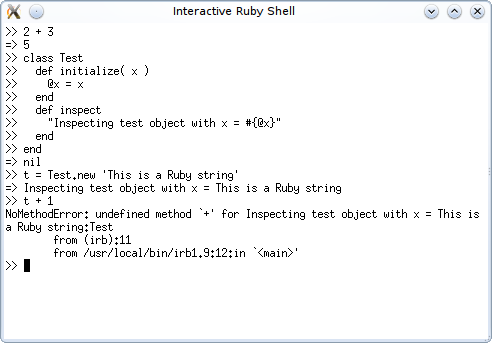
\includegraphics{irb}}
    \caption{Interactive Ruby Shell\label{fig:irb}}
  \end{center}
\end{figure}
\ac{IRB} accepts Ruby expressions and interprets them in the same context. After evaluating the expression, \ac{IRB} calls \code{\#inspect} on the result and prints the string returned by that method. \Eg if the user inputs \code{2 + 3}, \ac{IRB} will call \code{5.inspect} which returns \code{"5"}. The unquoted string then will be printed to standard output (here prefixed with ``=$>$''). \fig{irb} furthermore illustrates how in the case of an error, \ac{IRB} simply catches the exception and prints it to standard output instead.
% By defining \code{\#inspect} one can add self-documenting output to Ruby classes. \lst{narray} for example shows the formatted output generated by \code{NArray\#inspect}. % how can the reader know this!

\subsection{Object-Oriented, Single-Dispatch}
Ruby is object-oriented with single-dispatch. \Ie every object is an instance of a class and the class defines which methods and attributes an object supports. Ruby is purely object-oriented in the sense that everything including arrays, integers, floating point numbers, and classes is an object.

Ruby has open classes. \Ie it is possible to add methods to a class at any point in time. \lst{dispatch} shows an example where the already existing \code{Numeric} class is extended with a \code{plus} method (lines 1 to 5). Afterwards the method is called (line 6).
\lstset{language=Ruby,frame=single,numbers=left}
\begin{lstlisting}[float=htbp,caption={Method dispatch in Ruby},label=lst:dispatch]
class Numeric
  def plus(x)
    self.+ x
  end
end
y = 5.plus 6
# 11
\end{lstlisting}

However there are operations in Ruby which are not overloadable. \lst{nodispatch} gives several examples of operations (logical and, logical or, conditional statements) which have a behaviour which cannot be changed from within the Ruby language.
\begin{lstlisting}[float=htbp,caption={Methods in Ruby which are not overloadable},label=lst:nodispatch]
false and true
# false
false or true
# true
3 < 4 ? '3 is less than 4' : '3 is not less than 4'
# "3 is less than 4"
if true
  1
else
  2
end
# 1
\end{lstlisting}
The advantage of this is that programs are easier to understand since certain statements always have the expected behaviour. However this limits the meta programming capabilities of Ruby. This problem will be revisited in \sct{transjit}.

\subsection{Dynamic Typing}\label{cha:dynnum}
Ruby uses dynamic typing. In \lst{dynamic} the method \code{test} is defined.
\lstset{language=Ruby,frame=single,numbers=left}
\begin{lstlisting}[float=htbp,caption={Dynamic typing in Ruby},label=lst:dynamic]
def test(a, b)
  a + b
end
x = test 3, 5
# 8
x = test 'a', 'b'
# 'ab'
x = test 3, 'b'
# TypeError: String can't be coerced into Fixnum
\end{lstlisting}
Since Ruby is a dynamically typed language, it is possible to pass objects of any type as parameters. However the object passed for parameter \code{a} must support the method \code{+} and this method must accept one argument (the definition of method \code{test} is based on this). In a statically typed language an erroneous argument would cause an error message at compile time. In a dynamically typed language it will cause an exception at runtime (line 8).

\lstset{language=Ruby,frame=single,numbers=left}
\begin{lstlisting}[float,caption={Numerical types in Ruby},label=lst:mathn]
require 'mathn'
require 'complex'
require 'matrix'
x = -8 / 6                        
# -4/3
y = x * Complex(1, 2)             
# Complex(-4/3, -8/3)
z = 2 ** 40                       
# 1099511627776
y + z                             
# Complex(3298534883324/3, -8/3)
m = Matrix[[1, 2], [3, 4]]        
# Matrix[[1, 2], [3, 4]]
v = Vector[1/2, 1/3]              
# Vector[1/2, 1/3]
m * v                             
# Vector[7/6, 17/6]
z ** 2                            
# 1208925819614629174706176
\end{lstlisting}
\lst{mathn} shows how the Ruby standard library allows to combine integers, rational numbers, complex numbers, vectors, and matrices in a seamless way. \Eg line 6 shows a complex number with rational numbers as components. Note that Ruby uses dynamic typing to switch between native integers and big number representations in order to prevent numeric overflows. Implementing a comparable library in a statically typed language is hard because the type system has to reflect exactly which combinations of data types and operations are supported. If there are $n$ operations, there are potentially $2^n$ possible composite types, each of them supporting a different subset of operations.

Note that dynamic typing and weak typing are two different properties! Ruby uses strong, dynamic typing.

\subsection{Exception Handling}
Like many other programming languages, Ruby supports exceptions as a means of handling errors without using old-fashioned return codes. Thus the ``spaghetti logic'' that results from checking return codes can be avoided. \Ie exception handling facilitates separation of the code that detects the error and the code for handling the error without the semantic overhead of checking return values~\citep{RefWorks:541}. Exception handling is state-of-the art and supported by most modern programming languages (\eg C++, Java, Python, Ruby, and Smalltalk all support it).

\lstset{language=Ruby,frame=single,numbers=left}
\begin{lstlisting}[float=htbp,caption={Exception handling in Ruby},label=lst:exceptions]
begin
  print "Enter filename: "
  STDOUT.flush
  file_name = STDIN.readline.delete("\n\r")
  file = File.new file_name, 'r'
  # ...
rescue Exception => e
  puts "Error: #{e.message}"
end
\end{lstlisting}
\lst{exceptions} shows an example where the call to \code{File.new} in line 5 can potentially raise an exception. The exception is handled in the block starting after the \code{res\-cue} statement (lines 7 to 9). \Ie if an error occurs during the execution of lines 2 to 6, the program flow will continue in the rescue clause (lines 7 to 9).

\subsection{Garbage Collector}
The Ruby \ac{VM} uses the \emph{Mark \& Sweep}\index{Mark \& Sweep} algorithm as a garbage collector.
% Unlike reference counting, the \emph{Mark \& Sweep} algorithm is able to resolve cyclical references.
\begin{figure}[htbp]
  \begin{center}
    \resizebox{.7\textwidth}{!}{\begin{picture}(0,0)
        \input{mark-n-sweep.pstex_t}
      \end{picture}
      \includegraphics{mark-n-sweep}}\\
    \caption{Mark \& Sweep garbage collector\label{fig:marknsweep}}
  \end{center}
\end{figure}
\fig{marknsweep}\footnote{\url{http://www.brpreiss.com/books/opus5/html/page424.html}} illustrates the algorithm. Every object has a mark which initially is set to \code{false}. Starting from the root context, the graph of references is traversed recursively and every object encountered is marked with \code{true}. Afterwards all objects which are still marked \code{false} are deallocated. Cyclical references are not a problem since only objects connected to the root context are marked as \code{true}.
% A future Ruby \ac{VM} will probably include more advanced garbage collectors~\citep{ko2009} such as compacting garbage collectors and generational garbage collectors.

\subsection{Control Structures}
Ruby supports control structures for branching (see \fig{conditionals}) and looping (see \fig{loops}). The syntax of Ruby offers many different ways to write code with the same semantics. This requires the software developer to make frequent choices. But the advantage is that the software developer has more control over the appearance of the code. % \Ie Ruby has very good support for creating internal DSL\footnote{\url{http://en.wikipedia.org/wiki/Domain-specific_language}}. % do not understand how you come to the conclusion!
\begin{figure}[htbp]
  \lstset{language=Ruby,frame=single,numbers=none}
  \begin{center}
    \begin{minipage}[c]{.3\textwidth}
      \begin{lstlisting}
if x < 5 then
  statement1
end
      \end{lstlisting}
    \end{minipage}\hspace{1ex}
    \begin{minipage}[c]{.3\textwidth}
      \begin{lstlisting}
if x < 5 then
  statement1
else
  statement2
end
      \end{lstlisting}
    \end{minipage}\hspace{1ex}
    \begin{minipage}[c]{.3\textwidth}
      \begin{lstlisting}
statement1 if y == 3
      \end{lstlisting}
    \end{minipage}\\
    \begin{minipage}[c]{.3\textwidth}
      \begin{lstlisting}
unless x >= 5 then
  statement1
end
      \end{lstlisting}
    \end{minipage}\hspace{1ex}
    \begin{minipage}[c]{.3\textwidth}
      \begin{lstlisting}
unless x < 5 then
  statement2
else
  statement1
end
      \end{lstlisting}
    \end{minipage}\hspace{1ex}
    \begin{minipage}[c]{.3\textwidth}
      \begin{lstlisting}
statement1 unless y != 3
      \end{lstlisting}
    \end{minipage}
  \end{center}
  \caption{Conditional statements in Ruby~\citep{RefWorks:541}\label{fig:conditionals}}
\end{figure}
\begin{figure}[htbp]
  \lstset{language=Ruby,frame=single,numbers=none}
  \begin{center}
    \begin{minipage}[c]{.3\textwidth}
      \begin{lstlisting}
while cond do
  statement
end
      \end{lstlisting}
    \end{minipage}\hspace{1ex}
    \begin{minipage}[c]{.3\textwidth}
      \begin{lstlisting}
until cond do
  statement
end
      \end{lstlisting}
    \end{minipage}\hspace{1ex}
    \begin{minipage}[c]{.3\textwidth}
      \begin{lstlisting}
for x in array do
  statement
end
      \end{lstlisting}
    \end{minipage}\\
    \begin{minipage}[c]{.3\textwidth}
      \begin{lstlisting}
array.each do |x|
  statement
end
      \end{lstlisting}
    \end{minipage}\hspace{1ex}
    \begin{minipage}[c]{.3\textwidth}
      \begin{lstlisting}
loop do
  statement
  break if cond
end
      \end{lstlisting}
    \end{minipage}\hspace{1ex}
    \begin{minipage}[c]{.3\textwidth}
      \begin{lstlisting}
loop do
  statement
  break unless cond
end
      \end{lstlisting}
    \end{minipage}\\
    \begin{minipage}[c]{.3\textwidth}
      \begin{lstlisting}
for i in 0 .. n - 1 do
  statement
end
      \end{lstlisting}
    \end{minipage}\hspace{1ex}
    \begin{minipage}[c]{.3\textwidth}
      \begin{lstlisting}
for i in 0 ... n do
  statement
end
      \end{lstlisting}
    \end{minipage}\hspace{1ex}
    \begin{minipage}[c]{.3\textwidth}
      \begin{lstlisting}
array.each_index do |i|
  statement
end
      \end{lstlisting}
    \end{minipage}
  \end{center}
  \caption{Loop constructs in Ruby~\citep{RefWorks:541}\label{fig:loops}}
\end{figure}

\subsection{Mixins}
Ruby mixins are a unifying concept for namespaces and interfaces. \Ie the \code{module}-statement in Ruby can be used to declare a namespace. \Eg the \code{Math}-module in Ruby contains constants such as \code{Math::PI} and methods such as \code{Math::cos} (or \code{Math.cos}). However Ruby modules can also be used to ``mix'' methods into a class~\citep{RefWorks:541}. When a Ruby module is included in a class, all the module's instance methods become available as methods in the class as well. In that case the mixed-in module effectively behaves as superclass~\citep{thomas2004programming}. \lst{mixins} shows an example where the mixin \code{TimesThree} providing the method \code{three\_times} is mixed into the \code{String} class.
\lstset{language=Ruby,frame=single,numbers=none}
\begin{lstlisting}[float=htbp,caption={Mixins in Ruby},label=lst:mixins]
module TimesThree
  def three_times
    self + self + self
  end
end
class String
  include TimesThree
end
'abc'.three_times      
# "abcabcabc"
\end{lstlisting}

\subsection{Closures}\label{cha:closures}
Closures are code blocks retaining the variable scope. \lst{closures} gives an example where a function returns a closure.
\lstset{language=Ruby,frame=single,numbers=left}
\begin{lstlisting}[float=htbp,caption={Closures in Ruby},label=lst:closures]
def inc(i)
  proc do |v|
    v + i
  end
end
t = inc 5                   
# <Proc:0xb742ed2c@(irb):3>
t.call 3                    
# 8
[1, 2, 3].collect do |x|
  x ** 2
end                         
# [1, 4, 9]
[1, 2, 3].inject do |v,x|
  v + x
end                         
# 6
\end{lstlisting}
Even after returning from the method \code{inc} (lines 1 to 5), the closure returned by that method (lines 2 to 4) still has access to the method parameter \code{i}.
\added{Note that while the vertical bar \code{|} is used to represent the absolute value in mathematical notation, in Ruby syntax it is used to denote the parameters of a block (see \tbl{vbar} for more detail).}
\begin{table}[t]
  \begin{center}
    \caption{Ruby notation\label{tbl:vbar}}\vspace{1em}
    \begin{tabular}{lcc}\toprule
      & \textbf{Ruby syntax} & \textbf{mathematical notation} \\\midrule
      function & \code{f = proc \{ |x| x * x \}} & $f(x)\acs{DEF}x^2$ \\
      absolute value & \code{x.abs} & $\left|x\right|$ \\\bottomrule
    \end{tabular}
  \end{center}
\end{table}
% \Ie Ruby does not simply have a linear stack. Instead Ruby has a spaghetti stack where each context itself is an object which needs to be handled by the garbage collector.% paragraph needs explanation!

\subsection{Continuations}
Ruby supports continuations. A continuation captures the current state of the process in a variable. \Ie the continuation offers a way to save the current program pointer and context. \lst{continuations} gives an example where two continuations are used to jump into and out of a method.
\lstset{language=Ruby,frame=single,numbers=left}
\begin{lstlisting}[float=htbp,caption={Continuations in Ruby},label=lst:continuations]
require 'continuation'
def test(c2)
  callcc do |c1|
    return c1
  end
  c2.call
end
callcc do |c2|
  c1 = test(c2)
  c1.call
end
\end{lstlisting}
The order of execution is as follows:
\begin{enumerate}
\item The method \code{test} is defined (lines 2--7) and later called in line 9
\item In line 4 the continuation \code{c1} is returned and execution resumes in line 10
\item Line 10 calls the continuation so that execution resumes in line 6
\item Line 6 calls the continuation \code{c2} so that execution resumes after line 11 (\ie the program terminates)
\end{enumerate}

Basic language features such as exception handling, fibers (cooperative mul\-ti-thread\-ing), and break statements can all be implemented using continuations.

\subsection{Introspection}
\lstset{language=Ruby,frame=single,numbers=left}
\begin{lstlisting}[float=htbp,caption={Introspection in Ruby},label=lst:introspection]
x = 5                       
# 5
x.class                     
# Fixnum
x.class.class               
# Class
x.class.superclass          
# Integer
x.is_a?(Fixnum)             
# true
Fixnum < Integer            
# true
5.respond_to?(:+)           
# true
5.methods.grep(/^f/).sort   
# ["floor", "freeze", "frozen?"]
\end{lstlisting}
Introspection allows the program to ``see'' itself. \lst{introspection} gives some examples querying information about objects and their types. Using the method \code{methods} it is possible to get an array with the names of the methods supported by an object (line 15).

\subsection{Meta Programming}\label{cha:metaprog}
Ruby supports meta programming. \Ie the interpreter provides means of modifying the program during run-time. \lst{meta} gives a few examples.
\lstset{language=Ruby,frame=single,numbers=left}
\begin{lstlisting}[float=htbp,caption={Meta programming in Ruby},label=lst:meta]
eval 'x=5'                                 
# 5
a = [1]
a.instance_eval do
  push 2
end                                        
# [1, 2]
a.send :push, 3                            
# [1, 2, 3]
Object.const_get('String').class_eval do
  define_method 'test' do
    reverse
  end
end
'abc'.test                                 
# 'cba'
\end{lstlisting}
Using \code{eval} one can evaluate strings (line 1), using \code{instance\_eval} (lines 4--6) and \code{class\_eval} (lines 10--14) one can evaluate code blocks in the context of a particular object or class, and using \code{define\_method} one can create a method with the specified name and code block (lines 11--13).

Ruby meta programming is not as powerful as meta programming in Lisp or Smalltalk. \Eg some control structures such as while-loops and if-then-else statements cannot be overloaded which means that their behaviour cannot be changed.

\subsection{Reification}
Ruby supports some means of reification. Reification means that the program can modify the behaviour of the interpreter. By overloading the standard method \code{method\_missing} one can implement a different behaviour for the case an unknown method was called. \Eg \lst{reification} shows a definition of \code{Numeric\#method\_missing} (lines 2 to 10) which tries to find and call a method with the same prefix as the missing method.
\lstset{language=Ruby,frame=single,numbers=left}
\begin{lstlisting}[float=htbp,caption={Reification in Ruby},label=lst:reification]
class Numeric
  def method_missing(name, *args)
    prefix = Regexp.new("^#{name}")
    full_name = methods.find { |id| id =~ prefix }
    if full_name
      send(full_name, *args)
    else
      super
    end
  end
end
5.mod 2 
# calls 5.modulo 2
\end{lstlisting}
When the missing method \code{Numeric\#mod} is called in line 12, \code{Numeric\#method\_missing} is called which will call \code{Numeric\#modulo} instead.

There are other hooks for handling missing constant (\code{const\_missing}), inheritance changes (\code{inherited}), module inclusions (\code{extend\_object}), and method definitions (\code{method\_added})~\citep{RefWorks:541}.

\subsection{Ruby Extensions}\label{cha:rubyext}
Ruby has a C-\acs{API} for developing Ruby extensions\footnote{\url{http://www.rubyist.net/~nobu/ruby/Ruby_Extension_Manual.html}}. Compared to other \acp{API} such as the Java Native Interface (JNI) it is very easy to use. The problem of the current \ac{API} is that it does not allow for relocation of allocated memory~\citep{ko2009} (such as required by compacting garbage collectors).

\lst{sitelib} shows a small Ruby extension which upon loading registers the method \code{Numeric\#logx}. The Ruby native interface provides type definitions (\eg \code{VALUE}), macros (\eg \code{NUM2DBL}, \code{RUBY\_METHOD\_FUNC}), and methods (\eg \code{rb\_define\_method}, \code{rb\_float\_new}, $\ldots$) to manipulate the objects of the Ruby interpreter.
\lstset{language=C,frame=single,numbers=left}
\begin{lstlisting}[float=htbp,caption={Example of a C-extension for Ruby},label=lst:sitelib]
// gcc -shared -fPIC -I/usr/lib/ruby/1.8/x86_64-linux \
//     -o myextension.so myextension.c
#include <ruby.h>
#include <math.h>

VALUE wrap_logx(VALUE self, VALUE x)
{
  return rb_float_new(log(NUM2DBL(self)) / log(NUM2DBL(x)));
}

void Init_myextension(void) {
  VALUE numeric = rb_const_get(rb_cObject, rb_intern("Numeric"));
  rb_define_method(numeric, "logx", RUBY_METHOD_FUNC(wrap_logx), 1);
}
\end{lstlisting}
The Ruby extension needs to define a method where the method's name is the base name of the library prefixed with \code{Init\_} (here \code{Init\_myextension}). When the library is loaded using the \code{require} statement (see \lst{require}), this method is called so that the Ruby extension can register new methods (here: the method \code{Numeric\#logx}) with the Ruby interpreter.
\lstset{language=Ruby,frame=single,numbers=none}
\begin{lstlisting}[float=htbp,caption={Using the extension defined in \lst{sitelib}},label=lst:require]
require 'myextension'
# true
1024.logx 2
# 10.0
\end{lstlisting}

\subsection{Unit Testing}\label{cha:unittesting}
Unit testing is a common practise in the Ruby community~\citep{martin2009}. There are several unit testing tools for Ruby. The basic Test::Unit\footnote{\url{http://ruby-doc.org/core/classes/Test/Unit.html}} framework is part of the Ruby standard library. Effective testing continues to play an important role in removing software defects~\citep{unittest}. Ideally unit tests are automated and run after every change. This makes it possible to identify bugs at an early stageor when refactoring the code, \ie when they are being introduced. \Eg \lst{unit} shows a unit test for the implementation of \code{Array\#+} defined in \lst{rop}.
\lstset{language=Ruby,frame=single,numbers=none}
\begin{lstlisting}[float=htbp,caption={Unit test for \code{Array\#+} defined in \lst{rop}},label=lst:unit]
require 'test/unit'
class TC_Array < Test::Unit::TestCase
  def test_plus
    assert_equal [[6, 6], [6, 6]], 
                 [[1, 2], [3, 4]] + [[5, 4], [3, 2]]
  end
end
# Loaded suite array_plus
# Started
# .
# Finished in 0.002186 seconds.
#
# 1 tests, 1 assertions, 0 failures, 0 errors
\end{lstlisting}

With sufficient test coverage a test suite can become an executable specification of the behaviour of a program. \Eg the RSpec\footnote{\url{http://rspec.info/}} project provides sets of tests for each version of Ruby in order to test different implementations of the Ruby \ac{VM} and measure their degree of compatibility.

\section{\acs{JIT} Compilers}\label{cha:jits}
The Ruby programming language is an interpreted, pure object-oriented, and dynamically typed general purpose programming language (see \sct{ruby}). Furthermore Ruby supports closures and meta-programming. Also Ruby has a straightforward \ac{API} for writing extensions. Finally Ruby currently is on place 11 of the Tiobe Programming Community Index\footnote{\url{http://www.tiobe.com/index.php/content/paperinfo/tpci/}}. However in order for developers of machine vision software to take advantage of the productivity gains offered by Ruby, it is necessary to address the performance issue (see \fig{arraybench} on page \pageref{fig:arraybench}).

\subsection{Choosing a \acs{JIT} Compiler}
Since Ruby supports meta-programming, a \ac{JIT} compiler in general is indispensable for the perfomant execution of Ruby programs. \tbl{jits} shows several software projects which can be used to perform \ac{JIT} compilation.
\begin{table}[t]
  \begin{center}
    \caption{Just-in-time compilers\label{tbl:jits}}\vspace{1em}
    \begin{tabular}{lcccccc}\toprule
      & \begin{sideways}LLVM\end{sideways} &
      \begin{sideways}libJIT\end{sideways} &
      \begin{sideways}RubyInline\end{sideways} &
      \begin{sideways}lightning\end{sideways} &
      \begin{sideways}Asmjit\end{sideways} &
      \begin{sideways}Xbyak\end{sideways}\\\midrule
      register allocation   & \tick & \tick & \tick & \xxxx & \xxxx & \xxxx\\
      platform independence & \tick & \tick & \tick & \tick & \xxxx & \xxxx\\
      optimisation          & \tick & \xxxx & \tick & \xxxx & \xxxx & \xxxx\\\bottomrule
    \end{tabular}
  \end{center}
\end{table}
As one can see, the level of support varies greatly. Of the projects shown in \tbl{jits} only the \ac{LLVM} project by \citet{RefWorks:566} and the RubyInline\footnote{\url{http://rubyforge.org/projects/rubyinline}} approach support all the desired properties.
% The Rubinius\footnote{\url{http://rubini.us/}} Ruby \ac{VM} makes use of \ac{LLVM}. % what is this? introduce?
\begin{itemize}
\item \textbf{register allocation:} the \ac{JIT} compiler should provide an abstract machine with an infinite number of registers
\item \textbf{platform independence:} the \ac{JIT} compiler should be able to generate code for at least x86, x86-64, and ARM
\item \textbf{optimisation:} the \ac{JIT} compiler should provide code optimisation (preferably global optimisation)
\end{itemize}
Note that \tbl{jits} is not complete. However the other \ac{JIT} compilers are not readily available as a free software library with a dedicated \ac{API}.
%The JRuby\footnote{\url{http://www.jruby.org/}} Ruby \ac{VM} is based on the \ac{JVM} which in turn makes use of the HotSpot \ac{JIT} compiler.

The libJIT API is worth studying because it offers insights in what constitutes a \ac{JIT} compiler. The Ludicrous project\footnote{\url{http://rubystuff.org/ludicrous/}} provides a Ruby \ac{API} to use the libJIT just-in-time compiler library. However the Ruby \ac{API} does not support pointer operations.

After initially working with libJIT, in the end the RubyInline approach was chosen for the work of this thesis.  The C language together with the Ruby extension API is a stable interface for \ac{JIT} compilation. Also the GNU C compiler offers state of the art optimisation which facilitates competitive performance. The C code is generated at runtime and an ordinary \ac{AOT} compiler is called to produce a \ac{DLL} which can be loaded on-the-fly.

Note that the Ricsin project \citep{ricsin1,ricsin2} also provides a means of embedding C code into Ruby programs as well. However it requires the C code to be available \ac{AOT}.

\subsection{libJIT \acs{API}}
This section gives a small introduction to libJIT for the interested reader.

\lst{ctest} and \lst{jittest} show a basic array operation implemented directly in C and implemented using libJIT. The operation takes an array as argument (line 12 of \lst{jittest}) and increments every element of that array by one (line 23--31).
\lstset{language=C,frame=single,numbers=none}
\begin{lstlisting}[float=htbp,caption={Array operation implemented in C},escapechar=\$,label=lst:ctest]
// g++ -o ctest ctest.c
#include <stdlib.h>
#define SIZE 1000000
unsigned char *f(unsigned char *p, unsigned char one, unsigned char *pend)
{
  for ( ; p != pend; p++ )
    *p += one;
  return p;
}
int main(void)
{
  unsigned char *data = malloc(SIZE * sizeof(unsigned char));
  f(data, 1, data + SIZE);
  free(data);
  return 0;
}
\end{lstlisting}
\lstset{language=C,frame=single,numbers=left}
\begin{lstlisting}[float=htbp,caption={Array operation compiled with libJIT},escapechar=\$,label=lst:jittest]
// gcc -o jittest jittest.c -ljit
#include <stdlib.h>
#include <jit/jit.h>
#define SIZE 1000000
int main(void)
{
  // Compile function
  jit_context_t context = jit_context_create();
  jit_context_build_start(context);
  jit_type_t params[3];
  params[0] = jit_type_void_ptr;
  params[1] = jit_type_int;
  params[2] = jit_type_void_ptr;
  jit_type_t signature =
    jit_type_create_signature(jit_abi_cdecl, jit_type_void_ptr,
                              params, 3, 1);
  jit_function_t function = jit_function_create(context, signature);
  jit_value_t p, px, one, end, eq;
  jit_label_t start = jit_label_undefined;
  p = jit_value_get_param(function, 0);
  one = jit_value_get_param(function, 1);
  end = jit_value_get_param(function, 2);
  jit_insn_label(function, &start);
  jit_value_t temp1 = jit_insn_load_relative(function, p, 0, jit_type_ubyte);
  jit_value_t temp2 = jit_insn_add(function, temp1, one);
  jit_value_t temp3 = jit_insn_convert(function, temp2, jit_type_ubyte, 0);
  jit_insn_store_relative(function, p, 0, temp3);
  jit_value_t temp4 = jit_insn_add_relative(function, p, sizeof(jit_ubyte));
  jit_insn_store(function, p, temp4);
  eq = jit_insn_lt(function, p, end);
  jit_insn_branch_if(function, eq, &start);
  jit_insn_return(function, p);
  jit_function_compile(function);
  jit_context_build_end(context);
  // Call function
  unsigned char *data = malloc(SIZE * sizeof(unsigned char));
  void *args[3];
  jit_ptr arg1 = data;
  jit_ubyte arg2 = 1;
  jit_ptr arg3 = data + SIZE;
  jit_ptr result;
  args[0] = &arg1;
  args[1] = &arg2;
  args[2] = &arg3;
  jit_function_apply(function, args, &result);
  free(data);
  // Destruct function
  jit_context_destroy(context);
  return 0;
}
\end{lstlisting}
This is performed by sequentially loading each element (line 24), adding one to it (line 25), and writing it back to memory (line 27). The array pointer is incremented (line 28--29) and a conditional branch (line 30--31) is used to continue with the next element until the whole array was processed.

The example demonstrates how the libJIT library exposes the \ac{JIT} compiler functionality using the following data structures:
\begin{enumerate}
\item a \ac{JIT} context object keeping the functions
\item functions with parameters, instructions, and return value
\item values (virtual registers) of different types
  \begin{itemize}
  \item integers
  \item floating point numbers
  \item pointers
  \end{itemize}
\item labels
\end{enumerate}
The methods of the libJIT library expose the functionality of a complete compiler:
\begin{enumerate}
\item creating and destructing the context
\item defining functions and their arguments
\item adding \textbf{instructions}
  \begin{itemize}
  \item setting virtual registers to a constant
  \item loading values into a virtual register and writing values back to memory
  \item logical and mathematical operations
  \item control flow statements (\eg conditional branching)
  \end{itemize}
\item creating labels to jump to
\item allocating virtual registers and constants
\item compiling and calling methods
\end{enumerate}
%The libJIT library shows that it requires only few structurally different instructions to define a Turing-capable abstract machine.% I do not see how you arrive at this conclusion!
%This insight will be used in the next chapter to define a DSL for specifying native operations in the dynamically typed programming language Ruby.

\section{Summary}\label{cha:sumstate}
This chapter has highlighted some basic difficulties with implementing machine vision systems. It was shown that \ac{AOT} compilation of basic image processing operations is not feasible to due the large number of combinations of methods and parameter types. It was also shown that dynamic typing facilitates much more concise code than static typing.

The properties of the Ruby programming language were discussed. The Ruby programming language is an interpreted language. It is pure object-oriented and dynamically typed. It supports exception handling, mixins, and closures. Furthermore there is support for continuations and meta-programming. % Finally the Ruby \ac{VM} has a native interface which is easier to use than the native interfaces of most other \acp{VM}.% not sure you have shown this.
% Chapter 2: Ask yourself what am I doing here:
%            * showing advantages/disadvantages of Ruby
%            * present what would be dirable for the future in Ruby

Finally the choice of a \ac{JIT} compiler was discussed. It was decided to use \acs{GNU} C as a \ac{JIT} compiler because the C language represents a stable interface. Also the \acs{GNU} C compiler comes with a powerful optimiser.

\begin{savequote}[8cm]
  \begin{singlespace}
    ``Programming languages: performance, productivity, generality - pick any two.''
    \qauthor{Mario Wolczko}
    ``Elegance and familiarity are orthogonal.''
    \qauthor{Rich Hickey}
    ``In `Elephant' the programmer would write nothing about an array or database for storing reservations. Arrays of course would be necessary but the compiler would invent them.''
    \qauthor{John McCarthy}
  \end{singlespace}
\end{savequote}
\chapter{Handling Images in Ruby}\label{cha:rubyvision}
This chapter is about the core of the work presented in this thesis. \added{Since digital images are represented as \ac{2D} arrays, the way array operations are implemented is of great importance when developing machine vision systems. Most existing image processing libraries only support some combinations of operations and array element-types (also see \sct{statically})}. In this chapter \changed{an internal DSL}{a library} for manipulating uniform arrays is introduced. The \changed{DSL}{library} brings together performance and productivity in an unprecedented way (also see \sct{contrib}).
\begin{itemize}
\item transposing array views (\ie transposing an array ``without deep copy'' of elements)
\item lazy evaluation of array operations (\ie avoiding unnecessary memory-\acs{I}/\acs{O} for intermediate results)
\item \ac{JIT} compilation of array operations to achieve real-time performance
\end{itemize}

A set of objects is introduced to represent arrays, array views, and lazy evaluations in a modular fashion.
\begin{itemize}
\item \sct{transjit} explains how meta-programming can be used to integrate a \ac{JIT} compiler into the Ruby programming language
\item \sct{malloc} introduces memory objects
\item \sct{basictypes} defines native data types based on the memory objects
\item \sct{arrays} presents uniform arrays based on previously introduced objects
\item \sct{operations} introduces a \changed{DSL}{library} for describing computer vision algorithms
\item \sct{rubyvisionsum} gives a summary of this chapter
\end{itemize}
It is demonstrated how this approach facilitates succinct implementations of machine vision algorithms.

The software was published under the name Hornetseye. The software is provided as a set of packages \added{(see page \pageref{cha:software})}.

\section{Transparent \acs{JIT} Integration}\label{cha:transjit}
The performance of the Ruby \ac{VM} is significantly lower than the performance achieved with \acs{GNU} C (see \sct{dynlib}). One can achieve higher performance by introducing operations based on uniform arrays with native element types into the target language.

It is desirable to introduce a \ac{JIT} compiler without requiring the developer community to accept a modification of the Ruby language. In order to test the meta-programming capabilities of Ruby one can implement the method \code{\#method\_missing} as shown in \lst{reflect} (lines 7--13) in order to reflect on code instead of executing it.
\lstset{language=Ruby,frame=single,numbers=left}
\begin{lstlisting}[float=htbp,caption={Reflection using missing methods},escapechar=\$,label=lst:reflect,name=reflect]
class Const
  attr_accessor :inspect
  alias_method :to_s, :inspect
  def initialize(s)
    @inspect = s.to_s
  end
  def method_missing(name, *args)
    str = "#{ self }.#{ name }"
    unless args.empty?
      str += "(#{args.join ', '})"
    end
    Const.new str
  end
  def coerce(y)
    return Const.new(y), self
  end
end
\end{lstlisting}
Whenever an object of type \code{Const} receives a message for a method that is not implemented, it invokes the method \code{\#method\_missing} instead~\citep{RefWorks:541}. The method creates a textual representation of the method call as shown in \lst{refltest}. \lst{refltest} shows that the Ruby programming language supports changing the behaviour of unary negation (line 22), binary plus (line 24), and element access (line 26).
\lstset{language=Ruby,frame=single,numbers=left}
\begin{lstlisting}[float=htbp,caption={Example applying reflection to simple operations},escapechar=\$,label=lst:refltest,name=reflect]
a = Const.new 'a'
# a
b = Const.new 'b'
# b
-a
# a.-@
a + b
# a.+(b)
a[2]
# a[](2)
2 * a
# 2.*(a)
2 * a + b
# 2.*(a).+(b)
2 * (a + b)
# 2.*(a.+(b))
\end{lstlisting}

However \lst{refllimit} shows that meta programming support in Ruby is limited (also see \sct{metaprog}). \Eg the statement in line 34 returns \code{a} instead of \code{a.or(b)}.
\lstset{language=Ruby,frame=single,numbers=left}
\begin{lstlisting}[float=htbp,caption={Limitations of reflection in Ruby},escapechar=\$,label=lst:refllimit,name=reflect]
a or b
# a
a < b ? a : b
# a
b = a
# a
if a > b
  a -= b
end
# a.-(b)
begin
  a += 1
end until a > b
a
# a.+(1)
\end{lstlisting}
In order to implement transparent \ac{JIT} integration, it is therefore necessary to restrict the use of the programming language to a subset of Ruby with full meta programming support.

Some operations such as constructing the transpose of a \ac{2D} array merely require the data to be interpreted differently (in this case the order of array indices needs to be swapped). This can be achieved by deferring the calculation (\ie implementing support for \emph{lazy evaluation} \citep{abelson1996structure}). It turns out that this also makes it possible to avoid writing and reading intermediate results and to build tensor expressions.
% In order to compile code at run-time, one can use meta programming. \Ie the code first is compiled to C and then to machine code instead of running the code directly. \lst{reflect} shows a listing of how one can implement the method \code{\#method\_missing} in order to reflect on code instead of executing it. \lst{refltest} shows the principle in operation. Whenever a Ruby object receives a message for a method that isn't implemented in the receiver, it invokes the \code{\#method\_missing} method instead. One can use that to catch what would otherwise be an error, treating it as a normal method call~\citep{RefWorks:541}.
% \begin{itemize}
% \item constructor
% \item descriptor
% \item type (array-type)
% \item demand
% \item element
% \item variables
% \item strip
% \item subst
% \item compilable?
% \item ---
% \item store
% \item lookup
% \item skip
% \item slice
% \end{itemize}

\section{Malloc Objects}\label{cha:malloc}
In order to convert between native representation and Ruby values, the existing methods \code{Array\#pack}\footnote{\url{http://www.ruby-doc.org/ruby-1.9/classes/Array.html\#M000766}} and \code{String\#unpack}\footnote{\url{http://www.ruby-doc.org/ruby-1.9/classes/String.html\#M000659}} of the Ruby core library are used. \lst{pack} shows how Ruby values get converted to a Ruby string with a native representation of the values (line 3) and back (line 5).
\lstset{language=Ruby,frame=single,numbers=left}
\begin{lstlisting}[float=htbp,caption={Converting arrays to binary data and back},label=lst:pack]
array = [0x52, 0x75, 0x62, 0x79]
# [82, 117, 98, 121]
string = array.pack 'c' * 4
# "Ruby"
array = string.unpack 'c' * 4
# [82, 117, 98, 121]
\end{lstlisting}
% '[0x%x, 0x%x, 0x%x, 0x%x]' % array
% # "[0x52, 0x75, 0x62, 0x79]"
% "0x%x" % string.unpack('i')
% # "0x79627552"
The methods \code{Array\#pack} and \code{String\#unpack} require a template string as parameter which specifies the native data type(s) (see \tbl{directive}).
\begin{table}[htbp]
  \begin{center}
    \caption{Directives for conversion to/from native representation\label{tbl:directive}}\vspace{1em}
    \begin{tabular}{ll}\toprule
      \textbf{Directive} & \textbf{Native Data Type} \\\midrule
      C & Unsigned byte\\
      c & Byte\\
      d & Double-precision float\\
      f & Single-precision float\\
      I & Unsigned integer\\
      i & Integer\\
      Q & Unsigned long\\
      q & long\\
      S & Unsigned short\\
      s & Short\\\bottomrule
    \end{tabular}
  \end{center}
\end{table}

Since Ruby strings do not support pointer operations or multiple objects viewing the same memory location, \code{Malloc}-objects were introduced (as part of the work presented in this thesis). \code{Malloc} objects allow one to see a chunk of memory as an array of cubbyholes, each containing an 8-bit character (similar as \code{vector-ref} in Scheme~\citep{abelson1996structure}). \lst{malloc} shows an example using \code{Malloc} objects.
\lstset{language=Ruby,frame=single,numbers=none}
\begin{lstlisting}[float=htbp,caption={Manipulating raw data with Malloc objects},label=lst:malloc]
require 'malloc'
include Hornetseye
m = Malloc.new 4
# Malloc(4)
m.write 'abcd'
n = m + 2
# Malloc(2)
n.read 2
# "cd"
\end{lstlisting}
The method \code{Malloc\#+} is used to create a new object viewing a memory location with the given offset (also see \fig{memory} for a graphical illustration).
\begin{figure}[htbp]
  \begin{center}
    \resizebox{.2\textwidth}{!}{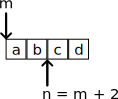
\includegraphics{memory}}
    \caption{Pointer operations (compare \lst{malloc})\label{fig:memory}}
  \end{center}
\end{figure}
An explanation of important methods is given in \tbl{malloc}.
\begin{table}[htbp]
  \begin{center}
    \caption{Methods for raw memory manipulation\label{tbl:malloc}}\vspace{1em}
    \begin{tabular}{ll}\toprule
      \textbf{Method} & \textbf{Description} \\\midrule
      \code{Malloc.new} & Allocate memory \\
      \code{Malloc\#read} & Read data from memory and return as string\\
      \code{Malloc\#write} & Write string data to memory\\
      \code{Malloc\#+} & Operation for doing pointer arithmetic\\\bottomrule
    \end{tabular}
  \end{center}
\end{table}

\section{Basic Types}\label{cha:basictypes}
As shown in \sct{dynlib}, in general an implementation using native data types can be optimised much better than an implementation using Ruby data types. In order to facilitate implementation of real-time machine vision software, representations of native types starting with booleans are introduced. Note that the type system is not part of the Ruby programming language or the Ruby core library. The type system was developed as part of the work presented in this thesis.

\subsection{Booleans}
In order to annotate a boolean value with type information, one can define a wrapper class for representing native booleans in Ruby (similar to ``boxing'' in Java\footnote{\url{http://eclipse.org/aspectj/doc/released/adk15notebook/autoboxing.html}}). \lst{bool1} shows the application of the class \code{BOOL}.
\lstset{language=Ruby,frame=single,numbers=left}
\begin{lstlisting}[float=htbp,caption={Boxing booleans},escapechar=\$,label=lst:bool1]
b = BOOL.new
# BOOL(false)
b.class
# BOOL
b[]
# false
b[] = true
# true
b
# BOOL(true)
\end{lstlisting}
The methods \code{[]} and \code{[]=} are used for getting (line 5) and setting (line 7) the boolean value encapsulated by an object of this class. The method \code{BOOL\#inspect} is used to define the textual representation for the output of Interactive Ruby.

\lstset{language=Ruby,frame=single,numbers=none}
\begin{lstlisting}[float=htbp,caption={Constructor short cut},escapechar=\$,label=lst:bool2]
b = BOOL true
# BOOL(true)
\end{lstlisting}
Although it is considered bad style to give Ruby methods a name starting with a capital letter, the language does not forbid this. This is sometimes used to define a short cut to a constructor such as for \code{BOOL.new} which then can be used as shown in \lst{bool2}.

In formal language one would define types and variables as shown in \equ{bool} using the boolean set $\acs{B}\acs{DEF}\{false,true\}$.
\begin{equation}\label{equ:bool}
  b\acs{IN}\acs{B}\mathrm{,\ }b=true
\end{equation}

\subsection{Integers}\label{cha:integers}
One can introduce classes to represent native integers in a similar fashion. However note that there are different types of native integers. \Ie current \acp{CPU} usually support 8-bit, 16-bit, 32-bit, and 64-bit signed and unsigned integers.
\lstset{language=Ruby,frame=single,numbers=left}
\begin{lstlisting}[float=htbp,caption={Template classes for integer types},escapechar=\$,label=lst:int]
INT 16, UNSIGNED
# USINT
INT(16, UNSIGNED).new 65535
# USINT(65535)
u = USINT.new 65535
# USINT(65535)
u = USINT 65535
# USINT(65535)
\end{lstlisting}
Using template classes one can achieve the behaviour shown in \lst{int}. By specifying the number of bits and the signed-ness one can instantiate an integer classes (\eg lines 1 and 3). \added{See \fig{uint} for a corresponding visual representation.}
\begin{figure}[htbp]
   \begin{center}
     \resizebox{.3\textwidth}{!}{\includegraphics{uint}}\\
     \caption{Abstract data type for 16-bit unsigned integer\label{fig:uint}}
   \end{center}
\end{figure}
Furthermore one can define type names and constructor shortcuts for certain integer types (\eg lines 5 and 7).

In formal language usually only integers (\acs{Z}) and non-negative integers (\acs{N0}) are distinguished. See \equ{int1} and \equ{int2} for examples.
\begin{equation}\label{equ:int1}
  i\acs{IN}\acs{Z}\mathrm{,\ }i=-123
\end{equation}
\begin{equation}\label{equ:int2}
  u\acs{IN}\acs{N0}\mathrm{,\ }u=234
\end{equation}

\subsection{Floating-Point Numbers}
\lstset{language=Ruby,frame=single,numbers=none}
\begin{lstlisting}[float=htbp,caption={Boxing floating point numbers},escapechar=\$,label=lst:float]
FLOAT SINGLE
# SFLOAT
FLOAT DOUBLE
# DFLOAT
FLOAT(SINGLE).new
# SFLOAT(0.0)
DFLOAT.new
# DFLOAT(0.0)
f = DFLOAT Math::PI
# DFLOAT(3.14159265358979)
\end{lstlisting}
Classes for representing single- and double-precision floating point numbers are implemented in a similar fashion as the integer classes. The behaviour of the implementation is shown in \lst{float}. \added{See \fig{float} for a visual representation of the floating point data types.}
\begin{figure}[htbp]
   \begin{center}
     \resizebox{.2\textwidth}{!}{\includegraphics{sfloat}}
     \resizebox{.215\textwidth}{!}{\includegraphics{dfloat}}\\
     \caption{Abstract data types for single-precision and double-precision floating point numbers\label{fig:float}}
   \end{center}
\end{figure}

The computer's representation of a double-precision floating point number consists of 64 bits. \Ie the hardware can represent $2^{64}$ different numbers. In mathematics the set of real numbers is uncountable and represented by the symbol \acs{R} (\eg see \equ{float}).
\begin{equation}\label{equ:float}
  \pi\acs{IN}\acs{R}\mathrm{,\ }\pi=3.1415926\ldots
\end{equation}

\subsection{Composite Numbers}
\lst{rgb1} demonstrates composite numbers such as \code{RGB} (for representing red, green, blue triplets) in Ruby.
\lstset{language=Ruby,frame=single,numbers=left}
\begin{lstlisting}[float=htbp,caption={Composite numbers},escapechar=\$,label=lst:rgb1]
c = RGB 4, 5, 6
# RGB(4,5,6)
c - 3 
# RGB(1,2,3)
7 - c
# RGB(3,2,1)
\end{lstlisting}
Note that the \ac{RGB} class supports left-handed (line 5) and right-handed (line 3) subtraction of a scalar. Right-handed subtraction of a scalar is handled by the method \code{RGB\#-}. In order to handle left-handed subtraction of a scalar, one has to implement the method \code{RGB\#coerce}. This method gets called by \code{Fixnum\#-} when it encounters an unknown data type. All numeric data types of the Ruby core library handle left-handed operations with an unknown data type in this way. This makes it possible to define data types at runtime and integrate them without having to change the implementation of existing data types. Examples of data types which are not part of the Ruby core are matrices and vectors.

Composite numbers are wrapped in a similar way as scalar numbers. \lst{rgb2} gives a few examples using the resulting \ac{API}.
\lstset{language=Ruby,frame=single,numbers=none}
\begin{lstlisting}[float=htbp,caption={Boxing composite numbers},escapechar=\$,label=lst:rgb2]
c = UBYTERGB RGB(1, 2, 3)
# UBYTERGB(RGB(1,2,3))
c = RGB(INT(16, UNSIGNED)).new RGB(1, 2, 3)
# USINTRGB(RGB(1,2,3))
c = RGB(FLOAT(SINGLE)).new RGB(0.1, 0.2, 0.3)
# SFLOATRGB(RGB(0.1,0.2,0.3))
\end{lstlisting}
\added{\fig{rgb} illustrates how the data types are composed.}
\begin{figure}[htbp]
   \begin{center}
     \resizebox{.3\textwidth}{!}{\includegraphics{ubytergb}}
     \resizebox{.3\textwidth}{!}{\includegraphics{usintrgb}}
     \resizebox{.15\textwidth}{!}{\includegraphics{sfloatrgb}}
     \caption{Composite types for unsigned byte RGB, unsigned short int RGB, and single-precision floating point RGB values\label{fig:rgb}}
   \end{center}
\end{figure}
%One can use \ac{3D} vectors to represent \ac{RGB} values. \equ{rgb} gives an example of a real-valued vector $\vec{c}$ with 3 components representing the red, green, and blue component of the \ac{RGB} value.% linear algebra: if you write this, you must show they make a vector field. !
%\begin{equation}\label{equ:rgb}
%  \vec{c}\acs{IN}\acs{R}^3\mathrm{,\ }\vec{c}=\begin{pmatrix}0.1\\0.2\\0.3\end{pmatrix}
%\end{equation}

\subsection{Pointers}
\added{Furthermore a pointer type is introduced. \Eg see \fig{pdfloat} showing how a pointer to a double precision floating point number is composed.}
\begin{figure}[htbp]
   \begin{center}
     \resizebox{.2\textwidth}{!}{\includegraphics{pdfloat}}\\
     \caption{Abstract data type for pointer to double precision floating point number\label{fig:pdfloat}}
   \end{center}
\end{figure}
The pointer encapsulates a \code{Malloc}-object. One can see a pointer object as a delayed fetch operation. \Ie the pointer object supports lazy evaluation of fetch operations.
In \cha{malloc} it was shown how the methods \code{Array\#pack} and \code{String\#unpack} convert between a Ruby value and a string with the native representation. \lst{pointer} shows how the methods \code{Pointer\_\#store} (line 3) and \code{Pointer\_\#demand} (lines 9 and 11) can be used to write/read boxed values to/from memory.
\lstset{language=Ruby,frame=single,numbers=left}
\begin{lstlisting}[float=htbp,caption={Pointer objects},escapechar=\$,label=lst:pointer]
p0 = Pointer(DFLOAT).new Malloc.new(16)
# *(DFLOAT)(Malloc(16))
p0.store DFLOAT(Math::PI)
# DFLOAT(3.14159265358979)
p1 = p0.lookup INT(1), INT(1)
# *(DFLOAT)(Malloc(8))
p1.store DFLOAT(Math::E)
# DFLOAT(2.71828182845905)
p0.demand
# DFLOAT(3.14159265358979)
p1.demand
# DFLOAT(2.71828182845905)
\end{lstlisting}
\Ie the pointer object handles reading and writing native values using the type information stored in its class. The method \code{Pointer\_\#lookup} (line 5) facilitates pointer operations in Ruby which are used as a basis for defining arrays later on.

\subsection{Ruby Objects}
\lstset{language=Ruby,frame=single,numbers=none}
\begin{lstlisting}[float=htbp,caption={Boxing arbitrary Ruby objects},escapechar=\$,label=lst:object1]
OBJECT 'Hello!'
# OBJECT("Hello!")
OBJECT 2 ** 127 - 1
# OBJECT(170141183460469231731687303715884105727)
\end{lstlisting}
In order to integrate the system of native types with the existing Ruby type system, a means of specifying non-native types is introduced. The class \code{OBJECT} is used to encapsulate Ruby objects which do not have a native representation as shown in \lst{object1}. Note that in practise one needs to define a class based on Ruby arrays which supports reading/writing values and pointer operations in a similar way to \code{Malloc} but providing this functionality for Ruby objects.

\section{Uniform Arrays}\label{cha:arrays}
A uniform array can be seen as a special case of a function accepting one or more indices as arguments and returning an array element as result. \added{\Eg \equ{sqrfun} shows a function returning the square of a value}\footnote{here the formal notation of the form $f:\left\{\begin{array}{ccl}X&\acs{TO}&Y\\x&\acs{MAP}&f(x)\end{array}\right.$ according to \citet{heus91} is used with $X$ and $Y$ being the domain and codomain of $f$}.
\begin{equation}\label{equ:sqrfun}
  f:\left\{\begin{array}{ccl}\{1, 2, 3\}&\acs{TO}&\acs{Z}\\x&\acs{MAP}&x^2\end{array}\right.
\end{equation}
\added{Since the function is defined on a finite set (\ie the set $\{1,2,3\}$), it can instead be defined using the function values $f(1)$, $f(2)$, and $f(3)$. \Ie $f$ can also be represented as an array, vector, or sequence (\eg the vector $f^\prime=(1\ 4\ 9)^\top$ with $f^\prime_1=1$, $f^\prime_2=4$, and $f^\prime_3=9$). Using the insight that matrices, arrays, vectors, and sequences are essentially different notations for functions, one can develop a representation which unifies these concepts}.

This section shows how variables, lambda terms, lookup objects, and the basic types introduced in the previous section can be used as building blocks to construct multi-dimensional arrays\removed{ and array views}.

\subsection{Variable Substitution}\label{cha:subst}
\lstset{language=Ruby,frame=single,numbers=left}
\begin{lstlisting}[float=htbp,caption={Variable objects and substitution},escapechar=\$,label=lst:variable1]
v1 = Variable.new INT
# Variable(INT)
v2 = Variable.new INT
# Variable(INT)
v2.subst v1 => INT(7)
# Variable(INT)
v2.subst v2 => INT(7)
# INT(7)
INT(5).subst v1 => INT(7)
# INT(5)
\end{lstlisting}
\lst{variable1} shows application of the variable class. The method \code{Variable\#subst} accepts a Ruby hash as argument (lines 5 and 7). It returns either a replacement for the object (line 8) or the object itself (line 6). By furthermore defining methods \code{INT\_\#subst}, \code{FLOAT\_\#subst}, \code{BOOL\_\#subst}, $\ldots$ and have them return \code{self}, one can achieve the behaviour shown in \lst{variable1} where applying a substitution to a scalar value has no effect (line 9). In formal language the substitutions shown in \lst{variable1} is specified using square brackets as shown in \equ{subst}~\citep{Church51,Mccarthy60recursivefunctions,barendregt1984introduction}.
\begin{align}\label{equ:subst}
  \begin{split}
    v_2\big[v_1\acs{DEF} 7\big]&\acs{EQV} v_1\\
    v_2\big[v_2\acs{DEF} 7\big]&\acs{EQV} 7\\
    5\big[v_1\acs{DEF} 7\big]&\acs{EQV} 5
  \end{split}
\end{align}

\subsection{Lambda Terms}\label{cha:lambda}
In $\lambda$-calculus the basic operations are \emph{abstraction} and \emph{application}~\citep{Church51,Mccarthy60recursivefunctions,barendregt1984introduction}. The concept of \emph{application} is also known as $\beta$-reduction. \added{\Eg \equ{alpha} shows the square function $x\acs{TO}x*x$ written in lambda notation. A dot is used to separate the bound variable $x$ from the term $x*x$.}
\begin{equation}\label{equ:alpha}
  \lambda x.x*x
\end{equation}
\added{\equ{beta} is an example of $\beta$-reduction. Here the square function is applied to the number $3$. The bound variable $x$ is replaced with the value $3$.}
\begin{equation}\label{equ:beta}
  (\lambda x.x*x)3\acs{BETA}(x*x)\big[x\acs{DEF} 3\big]\acs{TO}3*3\acs{TO}3
\end{equation}

\added{A \code{Lambda} class was implemented in order to facilitate manipulation of lambda expressions in Ruby. \lst{lambda1} shows application of the class \code{Lambda}.}
\lstset{language=Ruby,frame=single,numbers=left}
\begin{lstlisting}[float=htbp,caption={Lambda abstraction and application},escapechar=\$,label=lst:lambda1]
v = Variable.new INT
# Variable(INT)
l = Lambda.new v, v
# Lambda(Variable(INT),Variable(INT))
l.element INT(7)
# INT(7)
\end{lstlisting}
The identity function is used as an example to demonstrate abstraction and application. The variable \code{v} becomes a bound variable in the $\lambda$-term \code{l} (line 3). The same example written using the formal system of $\lambda$-calculus is shown in \equ{lambda}.
\begin{equation}\label{equ:lambda}
  (\lambda x.x)7\acs{BETA} x\big[x\acs{DEF} 7\big]\acs{EQV} 7
\end{equation}

\subsection{Lookup Objects}\label{cha:lookup}
In principle one can view a \ac{1D} array as a function accepting one argument. \Ie given a (typed) memory pointer $p$ and a stride $s$ one can define an arbitrary array $a$ as shown in \equ{array1}.
\begin{equation}\label{equ:array1}
  a:\left\{\begin{array}{ccl}\{0,1,\ldots,n-1\}&\acs{TO}&\acs{R}\\i&\acs{MAP}&fetch_{\acs{R}}(p+i*s)\end{array}\right.
\end{equation}
The function $fetch_{\acs{R}}$ is a pristine array representing physical memory (\eg memory of camera holding image data). Note that the array index is limited to a certain range, \ie $i\acs{IN}\{0,1,\ldots,n-1\}$.

\lstset{language=Ruby,frame=single,numbers=left}
\begin{lstlisting}[float=htbp,caption={Implementing arrays as lazy lookup},escapechar=\$,label=lst:array1]
v = Variable.new INDEX(INT(5))
# Variable(INDEX(INT(5)))
p = Pointer(DFLOAT).new Malloc.new(40)
a = Lambda.new v, Lookup.new(p, v, INT(1))
a[1] = 4.2
# 4.2
a[1]
# 4.2
\end{lstlisting}
\lst{array1} shows how an array is constructed using a pointer, a lookup object, and a lambda term. Line one creates an index variable. The size of the array becomes part of the type information of the variable (\ie \code{INDEX(INT(5))}). Line 3 allocates 40 bytes of memory and creates a pointer object for interpreting the memory as a sequence of double-precision floating point numbers. In line 4 the variable and the memory are used to create a lookup object. Finally the variable is bound using a lambda term.

By defining the Ruby operators \code{[]} and \code{[]=} one can implement element access. Element-access internally is implemented as beta-reduction (see \sct{lambda}). In practise the construction of arrays is hidden using the method \code{Sequence.new} as shown in \lst{array2}.
\lstset{language=Ruby,frame=single,numbers=none}
\begin{lstlisting}[float=htbp,caption={Uniform arrays},escapechar=\$,label=lst:array2]
a = Sequence.new DFLOAT, 5
a[1] = 4.2
# 4.2
a[1]
# 4.2
\end{lstlisting}

\subsection{Multi-Dimensional Arrays}\label{cha:multiarray}
One can treat a multi-dimensional array as a function accepting \emph{multiple} indices as arguments. \equ{ndim} shows the definition of an arbitrary \ac{3D} array $m$ using a memory pointer $p$ and the strides $s_0$, $s_1$, and $s_2$.
\begin{equation}\label{equ:ndim}
  m:\left\{\begin{array}{ccl}\{0,1,\ldots,n_2-1\}\acs{TIMES}\ldots\acs{TIMES}\{0,1,\ldots,n_0-1\}&\acs{TO}&\acs{R}\\(x_0\ x_1\ x_2)&\acs{MAP}&fetch_{\acs{R}}(p+s_2\,x_2+s_1\,x_1+s_0\,x_0)\end{array}\right.
\end{equation}
Internally the multi-dimensional array is represented by recursively nesting \code{Lambda} and \code{Lookup} objects. By extending the methods \code{[]} and \code{[]=} in a suitable manner and by introducing the method \code{MultiArray.new}, one can achieve the behaviour shown in \lst{multiarray}.
\lstset{language=Ruby,frame=single,numbers=left}
\begin{lstlisting}[float=htbp,caption={Multi-dimensional uniform arrays},escapechar=\$,label=lst:multiarray]
m = MultiArray.new UBYTE, 2, 4, 3
m[1, 2, 0] = 3
# 3
m[1, 2, 0]
# 3
m[0][2][1]
# 3
m[0][2][1] = 5
# 5
m[1, 2, 0]
# 5
\end{lstlisting}
The statement \code{MultiArray.new UBYTE, 2, 4, 3} in line 1 allocates a \ac{3D} array with $2\acs{TIMES} 4\acs{TIMES} 3$ elements. \fig{shape} illustrates the shape and the strides of the \ac{3D} array.
\begin{figure}[t]
  \begin{center}
    \begin{minipage}[c]{.22\textwidth}
      \begin{center}
        \begin{tabular}{cccc}\toprule
          i &
          \begin{sideways}$shape[i]$\end{sideways} &
          \begin{sideways}$strides[i]$\end{sideways} & 
          \begin{sideways}$x[i]$\end{sideways}\\\midrule
          0 & 2        & 1         & 1\\
          1 & 4        & 2         & 2\\
          2 & 3        & 8         & 0\\\bottomrule
        \end{tabular}\smallskip\\
        $strides[i]=\displaystyle\prod_{k=0}^{i-1}{shape[k]}$
      \end{center}
    \end{minipage}
    \begin{minipage}[c]{.28\textwidth}
      \resizebox{\textwidth}{!}{
        \begin{picture}(0,0)
          \input{strides.pstex_t}
        \end{picture}
        \includegraphics{strides}}
    \end{minipage}
    \caption{Shape and strides for a \acs{3D} array\label{fig:shape}}
  \end{center}
\end{figure}
The corresponding formal notation is given in \equ{arr3d}.
\begin{equation}\label{equ:arr3d}
  m:\left\{\begin{array}{ccl}\{0,1\}\acs{TIMES}\{0,1,2,3\}\acs{TIMES}\{0,1,2\}&\acs{TO}&\{0,1,\ldots,255\}\\(x_0\ x_1\ x_2)&\acs{MAP}&fetch_{\{0,1,\ldots,255\}}(p+s_2\,x_2+s_1\,x_1+s_0\,x_0)\end{array}\right.
\end{equation}
Note that the methods \code{[]} and \code{[]=} are defined in a fashion which makes it possible to specify either the major index first (\eg \code{m[0][2][1]} in line 6 of \lst{multiarray}) or the minor index first (\eg \code{m[1,2,0]} in line 4 of \lst{multiarray}). It is also possible to access the same element using hybrid notation (\eg \code{m[2,0][1]}). This makes it possible to interpret the \ac{3D} array of scalars as a \ac{2D} array $m^\prime$ of \ac{2D} vectors or as a \ac{2D} array $m^{\prime\prime}$ array of \ac{1D} functions. \changed{Ssee}{See} \equ{arr2d1d} for the corresponding formal domain specifications (the actual array definitions are omitted here for brevity).
\begin{align}\label{equ:arr2d1d}
  \begin{split}
    m^\prime&:\{0,1,2,3\}\acs{TIMES}\{0,1,2\}\acs{TO}\{0,1,\ldots,255\}^2\\
    m^{\prime\prime}&:\{0,1,2,3\}\acs{TIMES}\{0,1,2\}\acs{TO}\big(\{0,1\}\acs{TO}\{0,1,\ldots,255\}\big)
  \end{split}
\end{align}

\subsection{Array Views}
In the Ruby language the declaration \code{1 .. 5} is a short cut for \code{Range.new 1, 5, false}. Ranges are similar to intervals in mathematics, \eg $[1,5]$ in this case\footnote{$[a,b]$ denotes the closed interval from $a$ to $b$. \Ie $[a,b]\acs{DEF}\{x\acs{IN}\acs{R}|a\le x\le b\}$}. On the other hand \code{1 ... 6} is a short cut for \code{Range.new 1, 6, true} which is a \added{right-open} interval\removed{ where the endpoint is excluded}. The mathematical notation is $[1,6)$ in that case\footnote{$[a,b)$ denotes the right-open interval from $a$ to $b$. \Ie $[a,b)\acs{DEF}\{x\acs{IN}\acs{R}|a\le x<b\}$}. The method \code{[]} (and also the method \code{[]=}) can be extended so that they accept \code{Range} objects.

\lst{select} shows some examples where sub-arrays of a \ac{2D} array are specified using ranges. \added{Note that while the vertical bar \code{|} is used to represent the absolute value in mathematical notation, in Ruby syntax it is used to denote the parameters of a block (see \tbl{vbar} for more detail).}
\lstset{language=Ruby,frame=single,numbers=left}
\begin{lstlisting}[float=htbp,caption={Array views},escapechar=\$,label=lst:select]
m = lazy(5, 4) { |i,j| i + j * 5 }
# MultiArray(INT,2):
# [ [ 0, 1, 2, 3, 4 ],
#   [ 5, 6, 7, 8, 9 ],
#   [ 10, 11, 12, 13, 14 ],
#   [ 15, 16, 17, 18, 19 ] ]
u = m[1 .. 2]
# MultiArray(INT,2):
# [ [ 5, 10 ],
#   [ 6, 11 ],
#   [ 7, 12 ],
#   [ 8, 13 ],
#   [ 9, 14 ] ]
v = u[1 .. 3]
# MultiArray(INT,2):
# [ [ 6, 7, 8 ],
#   [ 11, 12, 13 ] ]
v = m[1 .. 3, 1 .. 2]
# MultiArray(INT,2):
# [ [ 6, 7, 8 ],
#   [ 11, 12, 13 ] ]
v = m[1 .. 2][1 .. 3]
# MultiArray(INT,2):
# [ [ 6, 7, 8 ],
#   [ 11, 12, 13 ] ]
\end{lstlisting}
Note that the order of the dimensions of the resulting array is cycled $n$ times where $n$ is the number of ranges specified. \Eg after declaring \code{m} in line 1, the values $5,6,7,\ldots$ appear in one row of the array. However extracting the sub array \code{u} (line 7) changes the order of the array indices so that the same elements now appear in one column.

\fig{select} illustrates the advantage of this semantics:
\begin{figure}[htbp]
  \begin{center}
    \resizebox{.6\textwidth}{!}{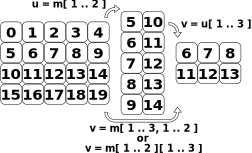
\includegraphics{select}}
    \caption{Extracting array views of a \acs{2D} array\label{fig:select}}
  \end{center}
\end{figure}
It allows one to specify the major indices first by invoking the operation \code{[]} twice and specifying the ranges separately (\eg \code{m[1 .. 2][1 .. 3]}). But it also allows one to specify the minor indices first by invoking the operation \code{[]} only once (\eg \code{m[1 .. 3, 1 .. 2]}).

The equivalent formal notation for the definition of the sub arrays $v$ is shown in \equ{subarr}.
\begin{equation}\label{equ:subarr}
  v:\left\{\begin{array}{ccl}\{0,1,2\}\acs{TIMES}\{0,1\}&\acs{TO}&\acs{Z}\\(x_0\ x_1)&\acs{MAP}&m(x_0+1,x_1+1)\end{array}\right.
\end{equation}

\section{Operations}\label{cha:operations}
\tbl{generic} gives an overview of generic array operations which can be found in computer vision algorithms.
\begin{table}[t]
  \begin{center}
    \caption{Generic set of array operations\label{tbl:generic}}
    \begin{tabular}{ll@{=}lc}\toprule
      & \multicolumn{2}{l}{operation} & array index\\\midrule
      read element                 & r       & a(b)             & -\\
      read sub-array               & r(i)    & a(i+b)           & i\\
      constant array               & r(i)    & a                & i\\
      index array                  & r(i)    & i                & i\\
      unary function               & r(i)    & f(a(i))          & i\\
      scalar-array binary function & r(i)    & f(a,b(i))        & i\\
      array-scalar binary function & r(i)    & f(a(i),b)        & i\\
      array-array binary function  & r(i)    & f(a(i),b(i))     & i\\
      accumulate                   & r       & f(r,a(i))        & i\\
      warp/mask                    & r(i)    & a(b(i))          & i\\
      unmask                       & r(b(i)) & a(i)             & i\\
      downsampling                 & r(i)    & a(b*i)           & i\\
      upsampling                   & r(b*i)  & a(i)             & i\\
      integral                     & r(i)    & r(i-1)+a(i)      & i\\
      map                          & r(i)    & b(a(i))          & i\\
      histogram                    & r(a(i)) & r(a(i))+1        & i\\
      weighted hist.               & r(a(i)) & r(a(i))+b(i)     & i\\
      convolution                  & r(i)    & r(i)+a(i-j)*b(j) & i,j\\\bottomrule
    \end{tabular}
  \end{center}
\end{table}
``a'' and ``b'' are parameters, and ``r'' is the result. Each of ``r'', ``a'', and ``b'' denotes a scalar or an array depending on the operation. In some cases a function ``f'' is involved. ``i'' and ``j'' are array indices. Note that this set of array operations is not complete since it does not cover operations involving multi-dimensional arrays (\eg matrix-vector multiplication). Also it is not minimal since an array-scalar binary function can be created using a constant array and an array-array binary function.

\subsection{Constant Arrays}\label{cha:const}
As shown in \sct{lookup}, one can see arrays as functions where the indices are the arguments of that function. A \ac{1D} constant array $carr$ where the value of each element is $0$ becomes a constant function as shown in \equ{const}.
\begin{equation}\label{equ:const}
  carr\acs{DEF}\lambda i.0
\end{equation}

Lines 4, 7, and 11 of \lst{const} show different ways of using the lambda class introduced in \cha{lambda} to create a function returning $0$.
\lstset{language=Ruby,frame=single,numbers=left}
\begin{lstlisting}[float=htbp,caption={Constant arrays},escapechar=\$,label=lst:const]
Lambda.new Variable.new(INDEX(INT(5))), UBYTE.new(0)
# Sequence(UBYTE):
# [ 0, 0, 0, 0, 0 ]
lazy(5) { 0 }
# Sequence(UBYTE):
# [ 0, 0, 0, 0, 0 ]
lazy(3, 2) { 0 }
# MultiArray(UBYTE,2):
# [ [ 0, 0, 0 ],
#   [ 0, 0, 0 ] ]
lazy(2) { lazy(3) { 0 } }
# MultiArray(UBYTE,2):
# [ [ 0, 0, 0 ],
#   [ 0, 0, 0 ] ]
\end{lstlisting}
Using closures it is possible to define the method \code{lazy}. The method accepts the shape of the array as argument and a closure for generating the array elements. \Eg one can construct a constant array using the statement \code{lazy(5) \{ 0 \}}. Note that it is possible to define multi-dimensional arrays by nesting calls to \code{lazy}.

\subsection{Index Arrays}
In practise index arrays can be useful (\eg for computing warp fields). In the \ac{1D} case the simplest index array is the identity function $id$ shown in \equ{index}.
\begin{equation}\label{equ:index}
  id\acs{DEF}\lambda i.i
\end{equation}

\lst{index} gives a few examples of index arrays and how they can be constructed using the \code{lazy} method.
\lstset{language=Ruby,frame=single,numbers=left}
\begin{lstlisting}[float=htbp,caption={Index arrays},escapechar=\$,label=lst:index]
x = lazy(3, 3) { |i,j| i }
# MultiArray(INT,2):
# [ [ 0, 1, 2 ],
#   [ 0, 1, 2 ],
#   [ 0, 1, 2 ] ]
y = lazy(3, 3) { |i,j| j }
# MultiArray(INT,2):
# [ [ 0, 0, 0 ],
#   [ 1, 1, 1 ],
#   [ 2, 2, 2 ] ]
idx = lazy(3, 3) { |i,j| i + j * 3 }
# MultiArray(INT,2):
# [ [ 0, 1, 2 ],
#   [ 3, 4, 5 ],
#   [ 6, 7, 8 ] ]
MultiArray(INT,2).indgen 3, 3
# MultiArray(INT,2):
# [ [ 0, 1, 2 ],
#   [ 3, 4, 5 ],
#   [ 6, 7, 8 ] ]
\end{lstlisting}
The index arrays \code{x} and \code{y} (lines 1 and 6) are useful for computing warp fields in practise. The class method \code{indgen} is a short cut for creating a multi-dimensional index array.

\subsection{Type Matching}
\begin{figure}[htbp]
  \begin{center}
    \resizebox{.45\textwidth}{!}{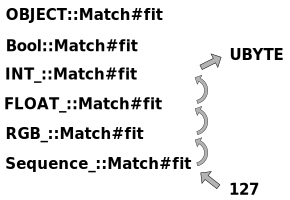
\includegraphics{matching}}
    \caption{Type matching\label{fig:matching}}
  \end{center}
\end{figure}
Type matching is introduced in order to conveniently convert Ruby values to native values. \fig{matching} illustrates how a Ruby value is passed on to the \code{Match\#fit} method of each native type class:
\begin{itemize}
\item \code{Sequence\_\#fit} rejects the value because it is not an array
\item \code{RGB\_\#fit} rejects the value because it is not an RGB value
\item \code{FLOAT\_\#fit} rejects the value because it is not a floating point number
\item \code{INT\_\#fit} accepts the value because it is an integer between $-2^{63}$ and $2^{64}-1$. The method returns \code{UBYTE} because this is the smallest native integer sufficient to hold the value \code{127}
\end{itemize}
\Ie the method \code{Match\#fit} determines whether the corresponding native type is the best fit for the given Ruby value. \lst{match} shows how this simplifies declarations of native arrays.
\lstset{language=Ruby,frame=single,numbers=none}
\begin{lstlisting}[float=htbp,caption={Type matching},escapechar=\$,label=lst:match]
Sequence[1, 2, 3]
# Sequence(UBYTE):
# [ 1, 2, 3 ]
Sequence[1, 2, -1]
# Sequence(BYTE):
# [ 1, 2, -1 ]
Sequence[1.5, RGB(1, 2, 3)]
# Sequence(DFLOATRGB):
# [ RGB(1.5,1.5,1.5), RGB(1.0,2.0,3.0) ]
MultiArray[[1, 2], [3, 4]]
# MultiArray(UBYTE,2):
# [ [ 1, 2 ],
#   [ 3, 4 ] ]
\end{lstlisting}

\subsection{Element-Wise Unary Operations}\label{cha:unary}
\lst{collect1} shows element-wise operations in Ruby. The method \code{Array\#collect} accepts a closure as argument which computes $2\,x+1$ for each element $x$ of the argument in this example.
\lstset{language=Ruby,frame=single,numbers=none}
\begin{lstlisting}[float=htbp,caption={Element-wise unary operations using \code{Array\#collect}},escapechar=\$,label=lst:collect1]
a = [1, 2, 3]
a.collect { |x| x * 2 + 1 }
# [3, 5, 7]
\end{lstlisting}
In order to facilitate more concise code, one can define methods which make it possible to use a shorter notation as shown in \lst{collect2}.
\lstset{language=Ruby,frame=single,numbers=none}
\begin{lstlisting}[float=htbp,caption={Short notation for element-wise operations},escapechar=\$,label=lst:collect2]
class Array
  def *(scalar)
    collect { |x| x * scalar }
  end
  def +(scalar)
    collect { |x| x + scalar }
  end
end
# $\textcolor{commentgray}{\emph{Example use}}$
a = [1, 2, 3]
a * 2 + 1
# [3, 5, 7]
\end{lstlisting}
The problem however is that eager evaluation will create intermediate results. \Eg evaluation of the statement \code{a * 2 + 1} will create the intermediate result \code{a * 2} and then add \code{1} to each element. \Ie an array to store the intermediate result is allocated and the values are written to it only to be read back again immediately. If one were to use lazy evaluation this would not happen (see \fig{intermediate}).
\begin{figure}[htbp]
   \begin{center}
     \begin{minipage}[t]{.336940298507463\textwidth} % 150.5
       \begin{center}
         \resizebox{\textwidth}{!}{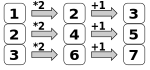
\includegraphics{eager}}\\
         eager evaluation
       \end{center}
     \end{minipage}
     \hspace{1cm}
     \begin{minipage}[t]{.263059701492537\textwidth} % 117.5
       \begin{center}
         \resizebox{\textwidth}{!}{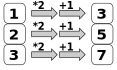
\includegraphics{lazy}}\\
         lazy evaluation
       \end{center}
     \end{minipage}
     \caption{Avoiding intermediate results by using lazy evaluation\label{fig:intermediate}}
   \end{center}
\end{figure}
\Ie in order to have concise code as well as performant code, it is important to facilitate lazy evaluation.

\lst{unary} shows how \emph{lazy} unary operations can be represented internally using objects (\eg of type \code{ElementWise(proc \{ |x| -x \}, :-@, proc \{ |t| t \})}).
\lstset{language=Ruby,frame=single,numbers=left}
\begin{lstlisting}[float=htbp,caption={Internal representation of unary operations},escapechar=\$,label=lst:unary]
s = Sequence(INT)[1, 2, 3]
# Sequence(INT):
# [ 1, 2, 3 ]
ElementWise(proc { |x| -x }, :-@, proc { |t| t.contiguous }).new s
# Sequence(INT):
# [ -1, -2, -3 ]
lazy { -s }
# Sequence(INT):
# [ -1, -2, -3 ]
lazy { |i| -s[i] }
# Sequence(INT):
# [ -1, -2, -3 ]
-s
# Sequence(INT):
# [ -1, -2, -3 ]
(-Sequence[:a, 1, :b])[1]
# NoMethodError: undefined method `-@' for :a:Symbol
lazy { -Sequence[:a, 1, :b] }[1]
# -1
\end{lstlisting}
\Ie, here the unary operation is characterised using following information
\begin{enumerate}
\item \code{proc \{ |x| -x \}}: A closure (see \sct{closures} with the operation to apply to each element
\item \code{:-@}: A unique symbol to identify the operation (for debugging purposes and to compute a cache key)
\item \code{proc \{ |t| t \}}: A closure for computing the data type of the result
\end{enumerate}
This representation is preserved when doing lazy evaluation (\eg when executing the statement \code{lazy \{ -s \}}).
When doing eager evaluation (the default) the operation will be applied to each element and the result is stored in a new array (\eg when executing the statement \code{-s}).
The difference between lazy and eager operations becomes visible when using operations in combination with element access. Line 16 \lst{unary} shows that eager evaluation of \code{-Sequence[:a, 1, :b]} will throw an exception since \code{:a} is a symbol and does not support negation. However it is possible to perform the operation lazily and extract the second element of the result without computing the other elements as shown in line 18.

\equ{unary} shows how one can use formal language to describe the application of a unary operator to an index array as an example.
\begin{equation}\label{equ:unary}
  -\big(\lambda i.i\big)=\lambda i.-i
\end{equation}
Note that in practise it is not necessary to normalise the expression. \Eg it is not a problem if \code{lazy \{ |i| -s[i] \}} and \code{lazy \{ -s \}} have different lazy representations.

\subsection{Element-Wise Binary Operations}\label{cha:binary}
\lstset{language=Ruby,frame=single,numbers=none}
\begin{lstlisting}[float=htbp,caption={Element-wise binary operations using \code{Array\#collect} and \code{Array\#zip}},escapechar=\$,label=lst:zip]
a = [1, 2, 3]
# [1, 2, 3]
b = [-1, 1, 3]
# [-1, 1, 3]
a.zip b
# [[1, -1], [2, 1], [3, 3]]
a.zip(b).collect { |x,y| x + y }
# [0, 3, 6]
\end{lstlisting}
\lst{zip} shows how one can perform element-wise addition of two arrays in Ruby. The method \code{Array\#zip}\footnote{\url{http://www.ruby-doc.org/core/classes/Array.html\#M002198}} merges elements of both arrays. Afterwards \code{Array\#collect} performs element-wise addition using the array of pairs as input.

Binary operations with support for \emph{lazy} evaluation are introduced in a similar fashion as unary operations. \Ie they are internally represented as objects (\eg of type \code{ElementWise(proc \{ |x,y| x + y \}, :+, proc \{ |t,u| t.coercion u \})}) and the representation is only preserved in lazy mode. In practise binary operations occur as array-array-, array-scalar-, and scalar-array-operations as one can see in \lst{binary}.
\lstset{language=Ruby,frame=single,numbers=none}
\begin{lstlisting}[float=htbp,caption={Internal representation of binary operations},escapechar=\$,label=lst:binary]
s = Sequence(INT)[1, 2, 3]
# Sequence(INT):
# [ 1, 2, 3 ]
ElementWise(proc { |x,y| x + y }, :+, proc { |t,u| t.coercion u }).
  new s, UBYTERGB(RGB(1, 2, 3))
# Sequence(INTRGB):
# [RGB(2,3,4), RGB(3,4,5), RGB(4,5,6)]
s + RGB(1, 2, 3)
# Sequence(INTRGB):
# [ RGB(2,3,4), RGB(3,4,5), RGB(4,5,6) ]
RGB(1, 2, 3) + s
# Sequence(INTRGB):
# [ RGB(2,3,4), RGB(3,4,5), RGB(4,5,6) ]
s + s
# Sequence(INT):
# [ 2, 4, 6 ]
\end{lstlisting}
In a similar fashion as in the case of unary operations, the binary operation is characterised by the following information
\begin{enumerate}
\item \code{proc \{ |x,y| x + y \}}: A closure with the operation to apply to each pair of elements
\item \code{:+}: A unique symbol to identify the operation (for debugging purposes and to compute a cache key)
\item \code{proc \{ |t,u| t.coercion u \}}: A closure for deriving the data type of the result
\end{enumerate}

\equ{binary} show examples of formal representation of array-scalar, scalar-array, and array-array binary operations.
\begin{align}\label{equ:binary}
  \begin{split}
    \big(\lambda i.f(i)\big)+c&\acs{EQV}\lambda i.f(i)+c\\
    c+\big(\lambda i.f(i)\big)&\acs{EQV}\lambda i.c+f(i)\\
    \big(\lambda i.f(i)\big)+\big(\lambda i.g(i)\big)&\acs{EQV}\lambda i.f(i)+g(i)
  \end{split}
\end{align}

Furthermore there are unary and binary methods. \Eg \code{Math.sqrt(x)} will compute the square root of $x$, \code{Math.atan2(y, x)} will compute the polar angle of $(x\ y)^\top$. However methods and operators are just different forms of notation for element-wise operations. \Ie they are handled the same way as element-wise operations.

\subsection{\acsp{LUT} and Warps}\label{cha:lutwarps}
\subsubsection{\acsp{LUT}}
Like any other array, one can understand a \ac{LUT} as a function. Element-wise lookup can be understood as element-wise application of that function. See \lst{lookup} for example.
\lstset{language=Ruby,frame=single,numbers=none}
\begin{lstlisting}[float=htbp,caption={Element-wise application of a \acs{LUT}},escapechar=\$,label=lst:lookup]
MultiArray[1, 2, 0].lut Sequence[:a, :b, :c]
# Sequence(OBJECT):
# [ :b, :c, :a ]
\end{lstlisting}

In general it is desirable to support multi-dimensional \acp{LUT}, \ie using vectors with multiple dimensions as lookup index. Furthermore it is possible to have \acp{LUT} with multi-dimensional arrays as elements. \equ{lookup1} shows application of the \ac{LUT} $l$ to the array $a$.
\begin{equation}\label{equ:lookup1}
  b(\vec{x})(\vec{y})=l\big(a(\vec{x})\big)(\vec{y})
\end{equation}
The array $a$ is interpreted as an $n_1$-dimensional array with $n_2$-dimensional vectors as elements. The $n_2$-dimensional vectors are used for a lookup with $l$. See \equ{lookup2} for the types of $a$, $l$, and the result $b$.
\begin{equation}\label{equ:lookup2}
a:\acs{N0}^{n_1}\acs{TO}\acs{N0}^{n_2}\mathrm{,\ }
l:\acs{N0}^{n_2}\acs{TO} (\acs{N0}^{n_3}\acs{TO} K)\mathrm{,\ }
b:\acs{N0}^{n_1}\acs{TO} (\acs{N0}^{n_3}\acs{TO} K)
\end{equation}

\lst{pseudo} shows how to use a \ac{LUT} for computing a pseudo colour image.
\lstset{language=Ruby,frame=single,numbers=left}
\begin{lstlisting}[float=htbp,caption={Creating a pseudo colour image},escapechar=\$,label=lst:pseudo]
class Numeric
  def clip(range)
    [[self, range.begin].max, range.end].min
  end
end
colours = Sequence.ubytergb 256
for i in 0...256
  hue = 240 - i * 240.0 / 256.0
  colours[i] =
    RGB(((hue - 180).abs -  60).clip(0...60) * 0xFF / 60.0,
        (120 - (hue - 120).abs).clip(0...60) * 0xFF / 60.0,
        (120 - (hue - 240).abs).clip(0...60) * 0xFF / 60.0)
end
MultiArray.load_ubyte(ARGV[0]).lut(colours).save_ubytergb ARGV[1]
\end{lstlisting}
First the \code{Numeric} class is extended with a method for clipping numbers to a certain range (lines 1--5). Then a colour palette with 256 elements is allocated (line 6) and populated with values (lines 7--13). \fig{palette} shows a plot of the colour channels of the resulting palette.
\begin{figure}[htbp]
  \begin{center}
    \begin{tikzpicture}[x=1.5cm,y=1cm,domain=0:8]
      \draw[very thin,color=gray] (-0.1,-0.1) grid (8.1,4.1);
      \draw[->] (-0.2,0) -- (8.2,0) node[right] {$x$};
      \draw[->] (0,-0.2) -- (0,4.2) node[above] {$y$};
      \foreach \x  in {0,...,8}{
        \pgfmathsetmacro\xtext{ \x * 32}
        \draw (\x,1pt) -- (\x,-1pt) node[below] {\tiny $\xtext$};
      }
      \foreach \y  in {0,...,4}{
        \pgfmathsetmacro\ytext{ \y * 64} 
        \draw (1pt,\y cm) -- (-1pt,\y cm) node[left]  {\tiny $\ytext$};
      }
      \draw[thick,color=red]   (0,0) -- (2,0) -- (4,0) -- (6,4) -- (8,4);
      \draw[color=red] (1,0) node[above] {red};
      \draw[color=red] (3,0) node[above] {red};
      \draw[color=red] (5,2) node[left] {red};
      \draw[color=red] (7,4) node[below] {red};
      \draw[thick,color=green] (0,0) -- (2,4) -- (4,4) -- (6,4) -- (8,0);
      \draw[color=green] (1,2) node[left] {green};
      \draw[color=green] (3,4) node[below] {green};
      \draw[color=green] (5,4) node[below] {green};
      \draw[color=green] (7,2) node[right] {green};
      \draw[thick,color=blue]  (0,4) -- (2,4) -- (4,0) -- (6,0) -- (8,0);
      \draw[color=blue] (1,4) node[below] {blue};
      \draw[color=blue] (3,2) node[right] {blue};
      \draw[color=blue] (5,0) node[above] {blue};
      \draw[color=blue] (7,0) node[above] {blue};
    \end{tikzpicture}
    \caption{Pseudo colour palette\label{fig:palette}}
  \end{center}
\end{figure}
Finally an image is loaded, element-wise lookup is performed, and the resulting image is written to disk (line 14). \fig{thermal} shows a thermal image used as input and the corresponding pseudo colour image created with afore mentioned program.
\begin{figure}[htbp]
  \begin{center}
    \begin{minipage}[t]{.45\textwidth}
      \begin{center}
        \resizebox{\textwidth}{!}{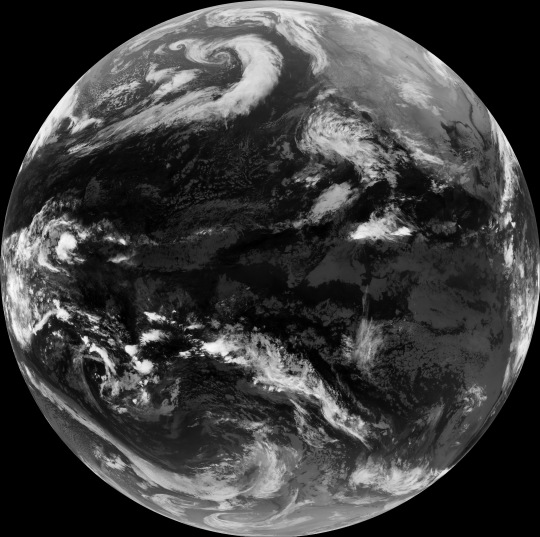
\includegraphics{goes}}\\
        input image
      \end{center}
    \end{minipage}
    \hspace{.5cm}
    \begin{minipage}[t]{.45\textwidth}
      \begin{center}
        \resizebox{\textwidth}{!}{\includegraphics{pseudo}}\\
        output image
      \end{center}
    \end{minipage}
    \caption{Thermal image displayed with pseudo colours (source: \href{http://visibleearth.nasa.gov/view_rec.php?id=1564}{NASA Visible Earth})\label{fig:thermal}}
  \end{center}
\end{figure}

\lst{pseudo} shows how the concepts introduced in previous chapters apply to implementation of image processing algorithms. The implementation of the pseudo colour visualisation is both concise and real-time capable.

\subsubsection{Warps}\label{cha:warps}
An image warp is essentially the same as element-wise lookup. \Ie the image is used as a \ac{LUT} and the input data is a \ac{2D} array of warp vectors. \lst{warp} shows how one can convert a topographical image from equirectangular to azimuthal projection.
\lstset{language=Ruby,frame=single,numbers=left}
\begin{lstlisting}[float=htbp,caption={Warp from equirectangular to azimuthal projection},escapechar=\$,label=lst:warp]
img = MultiArray.load_ubytergb 'world.jpg'
w, h = *img.shape
c = 0.5 * (h - 1)
x, y = lazy(h, h) { |i,j| i - c }, lazy(h, h) { |i,j| j - c }
radius = lazy { Math.hypot(x, y).to_int }
angle = lazy { ((Math.atan2(x, y) / Math::PI + 1) * w / 2).to_int }
[angle, radius].lut(img).save_ubytergb 'polar.jpg'
\end{lstlisting}
Note that in this example the components of the warp vectors are two separate arrays (\ie \code{angle} in line 6 and \code{radius} in line 5). The array class of the Ruby language was extended so that the expression \code{[angle, radius].lut(img)} (line 7) can be used to specify the arrays holding the components of the warp vectors.

\fig{warp} illustrates how the components of the warp vectors are constructed.
\begin{figure}[htbp]
  \begin{center}
    \begin{minipage}[t]{.22\textwidth}
      \begin{center}
        \framebox{\resizebox{\textwidth}{!}{
\includegraphics{warpx}}}\\
        $x_1$
      \end{center}
    \end{minipage}
    \hspace{.25cm}
    \begin{minipage}[t]{.22\textwidth}
      \begin{center}
        \framebox{\resizebox{\textwidth}{!}{
\includegraphics{warpy}}}\\
        $x_2$
      \end{center}
    \end{minipage}
    \hspace{.25cm}
    \begin{minipage}[t]{.22\textwidth}
      \begin{center}
        \framebox{\resizebox{\textwidth}{!}{
\includegraphics{warpa}}}\\
        $\angle(x_1,x_2)$
      \end{center}
    \end{minipage}
    \hspace{.25cm}
    \begin{minipage}[t]{.22\textwidth}
      \begin{center}
        \framebox{\resizebox{\textwidth}{!}{
\includegraphics{warpr}}}\\
        $\sqrt{x_1^2+x_2^2}$
      \end{center}
    \end{minipage}
    \caption{Visualised components of warp vectors\label{fig:warp}}
  \end{center}
\end{figure}
The visualisation was inspired by \citet{RefWorks:467}. Arrays with $x_1$ and $x_2$ values are used to construct arrays with the angle and radius of the azimuthal projection. The result of applying the warp is shown in \fig{polar}.
\begin{figure}[htbp]
  \begin{center}
    \begin{minipage}[t]{.6\textwidth}
      \begin{center}
        \framebox{\resizebox{\textwidth}{!}{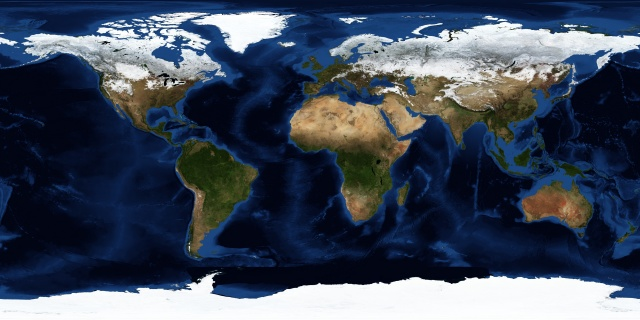
\includegraphics{world}}}\\
        input image
      \end{center}
    \end{minipage}
    \hspace{.5cm}
    \begin{minipage}[t]{.3\textwidth}
      \begin{center}
        \framebox{\resizebox{\textwidth}{!}{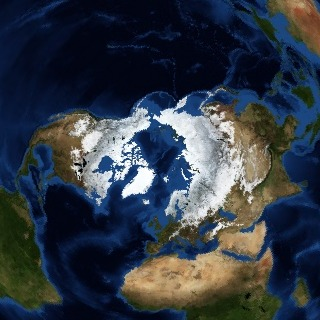
\includegraphics{polar}}}\\
        output image
      \end{center}
    \end{minipage}
    \caption{Warping a satellite image (source: \href{http://visibleearth.nasa.gov/view_rec.php?id=7100}{NASA Visible Earth})\label{fig:polar}}
  \end{center}
\end{figure}

\subsection{Injections}\label{cha:inject}
Apart from element-wise functions (\eg \acp{LUT}) one frequently encounters the \ac{foldl} operation in functional programming. The operation is also known as the $reduce$ part of Google's MapReduce implementation~\citep{laemmel2008google}. Given a binary function $A\acs{TO} B\acs{TO} B$ and a value of type $B$, the \ac{foldl} operation yields a function taking an array as argument which does cumulative application of the binary function~\citep{hutton1999fold} (see \equ{fold}).
\begin{align}\label{equ:fold}
  \begin{split}
    &(A\acs{TO} B\acs{TO} B)\acs{TO} B\acs{TO}\big((\acs{N0}\acs{TO} A)\acs{TO} B\big)\\
    &\acs{foldl}(f,v)([x_1,x_2,x_3,\ldots])=f(\ldots f(f(f(v,x1),x2),x3),\ldots)
  \end{split}
\end{align}
Note that \acs{foldl} is left-associative. When applying the fold operation to non-as\-so\-cia\-ti\-ve operations (\eg division or subtraction) it is important to distinguish between left-as\-so\-cia\-ti\-ve (\acs{foldl}) and right-associative folding (\ac{foldr}).
In Ruby the \ac{foldl} operation is known as \emph{injection}. \lst{inject1} shows two ways of specifying an injection for computing the product of all elements of an array.
\lstset{language=Ruby,frame=single,numbers=none}
\begin{lstlisting}[float=htbp,caption={Left-associative fold operation in Ruby},escapechar=\$,label=lst:inject1]
[2, 3, 5, 7, 11].inject(1) { |a,b| a * b }
# 2310
[2, 3, 5, 7, 11].inject 1, :*
# 2310
\end{lstlisting}
The equivalent formal expression using the product symbol is shown in \equ{prod}.
\begin{equation}\label{equ:prod}
  \prod_{i\acs{IN}\{1,2,\ldots,5\}}s_i\mathrm{\ where\ }s\acs{DEF}(2\ 3\ 5\ 7\ 11)
\end{equation}

\lst{inject2} shows how an injection can be represented internally using an object of class \code{Inject}.
\lstset{language=Ruby,frame=single,numbers=left}
\begin{lstlisting}[float=htbp,caption={Internal representation of injections},escapechar=\$,label=lst:inject2]
s = Sequence[2, 3, 5, 7, 11]
# Sequence(UBYTE):
# [ 2, 3, 5, 7, 11 ]
v = Variable.new INDEX(s.size)
# Variable(INDEX(INT(5)))
v1 = Variable.new INT
# Variable(INT)
v2 = Variable.new INT
# Variable(INT)
block = proc { |a,b| a * b }.call v1, v2
# *(Variable(INT),Variable(INT))
inject = Inject.new s.element(v), v, INT(1), block, v1, v2
# INT(2310)
Sequence[2, 3, 5, 7, 11].inject(1) { |a,b| a.to_int * b }
# 2310
\end{lstlisting}
The closure (or nameless function) \code{proc \{ |a,b| a * b \}} is converted to an object by passing it \code{Variable} objects as parameters (line 10). The end of the listing shows how the operation might be invoked in practise (line 14).

The image processing operations \code{min}, \code{max}, and \code{range} can be implemented using \ac{foldl} (see \lst{minmax}).
\lstset{language=Ruby,frame=single,numbers=none}
\begin{lstlisting}[float=htbp,caption={Various cumulative operations based on injections},escapechar=\$,label=lst:minmax]
m = MultiArray[[2, 3, 5], [7, 11, 13]]
# MultiArray(UBYTE,2):
# [ [ 2, 3, 5 ],
#   [ 7, 11, 13 ] ]
m.min
# 2
m.max
# 13
m.range
# 2..13
\end{lstlisting}
Injection can be implemented recursively. The injection is applied to each dimension separately. \Eg \fig{sum} shows the recursive computation of the sum of an array.
\begin{figure}[htbp]
   \begin{center}
     \resizebox{.6\textwidth}{!}{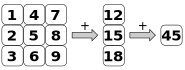
\includegraphics{inject}}\\
     \caption{Recursive implementation of injection (here: sum)\label{fig:sum}}
   \end{center}
\end{figure}
Other associative operations such as computing the maximum, minimum, or the product can be computed in the same recursive manner as well.

Using Ruby closures and \code{Variable} objects it is possible to develop a concise notation for sums. \Eg \ac{1D} and \ac{2D} sums as shown in \equ{sum}.
\begin{align}\label{equ:sum}
  \begin{split}
    u_i&\acs{DEF}\displaystyle\sum_{j=1}^2 m_{ji}\\
    v&\acs{DEF}\displaystyle\sum_{j=1}^2\sum_{i=1}^3 m_{ji}\mathrm{,\ }m\acs{IN}\acs{Z}^{3\acs{TIMES} 2}
  \end{split}
\end{align}
The corresponding Ruby code to compute $u$ and $v$ is shown in \lst{sums}.
\lstset{language=Ruby,frame=single,numbers=none}
\begin{lstlisting}[float=htbp,caption={Concise notation for sums of elements},escapechar=\$,label=lst:sums]
m = MultiArray[[2, 3, 5], [7, 11, 13]]
# MultiArray(UBYTE,2):
# [ [ 2, 3, 5 ],
#   [ 7, 11, 13 ] ]
u = sum { |i| m[i] }
# Sequence(UBYTE):
# [ 9, 14, 18 ]
v = sum { |i,j| m[i,j] }
# 41
\end{lstlisting}
Note that it is not even necessary to specify the ranges for the index variable because they can be inferred from the element access.

\subsection{Tensor Operations}\label{cha:tensor}
The \code{lazy} method and the \code{sum} operator (see \cha{const} and \cha{inject}) in combination with unary and binary element-wise operations (see \cha{unary} and \cha{binary}) are sufficiently generic to implement tensor operations. \lst{ftensor} shows a tensor operation implemented using the FTensor C++ library. The equivalent Ruby implementation is shown in \lst{rtensor}.
\lstset{language=Ruby,frame=single,numbers=none}
\begin{lstlisting}[float,caption={Tensor operations in Ruby (equivalent to \lst{ftensor})},label=lst:rtensor]
a = MultiArray.dfloat 3, 3
b = MultiArray.dfloat 3, 3
r = eager { |i,k| sum { |j| a[i,j] * b[j,k] } }
\end{lstlisting}
The \code{eager} performs the operation lazily the same way as the \code{lazy} method does. However it forces the result to be computed and stored in a new array.

\subsection{Argmax and Argmin}\label{cha:arg}
The definitions of the operations $\operatorname{argmax}$ and $\operatorname{argmin}$ are given in \equ{argmin} and \equ{argmax}
\begin{align}
  \mathop{\operatorname{argmin}}_{\vec{x}}\big(f(\vec{x})\big)&\acs{DEF}\big\{\vec{x}\,\big|\acs{FORALL}\vec{x^\prime}:f(\vec{x})\le f(\vec{x^\prime})\big\}\label{equ:argmin}\\
  \mathop{\operatorname{argmax}}_{\vec{x}}\big(f(\vec{x})\big)&\acs{DEF}\big\{\vec{x}\,\big|\acs{FORALL}\vec{x^\prime}:f(\vec{x})\ge f(\vec{x^\prime})\big\}\label{equ:argmax}
\end{align}
\added{where $\vec{x}$ is any coordinate in the $n$-dimensional input array $f$.}
The operations return the argument for which the function attains the maximum or the minimum value. \lst{argmax} shows three operations:
\lstset{language=Ruby,frame=single,numbers=left}
\begin{lstlisting}[float=htbp,caption={Argument maximum},escapechar=\$,label=lst:argmax]
m = MultiArray[[1, 2, 3], [4, 5, 9], [7, 8, 3], [7, 6, 4]]
# MultiArray(UBYTE,2):
# [ [ 1, 2, 3 ],
#   [ 4, 5, 9 ],
#   [ 7, 8, 3 ],
#   [ 7, 6, 4 ] ]
argmax { |i| m.unroll[i] }
# [Sequence(INT):
# [ 2, 2, 1, 0 ]]
m.warp argmax { |i| m.unroll[i] }.first, lazy(4) { |i| i }                
# Sequence(UBYTE):                                                                           
# [ 3, 9, 8, 7 ]
argmax { |i,j| m[i,j] }
# [2, 1]
\end{lstlisting}
\begin{enumerate}
\item \ac{1D} argmax for locating the maximum of each row (line \changed{7}{10})
\item Instruction for extracting the maxmimum of each row (line 10)
\item \ac{2D} argmax for locating the maximum \added{(line 13)}
\end{enumerate}
The listing demonstrates how to construct a warp for extracting the maximum of each row of the input array. Note that the argument operation returns an array (or several arrays) if the input array has more dimensions than the argument.

The argument functions are implemented recursively using warps as illustrated in \fig{argmax}.
\begin{figure}[htbp]
   \begin{center}
     \resizebox{\textwidth}{!}{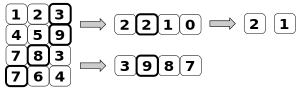
\includegraphics{argmax}}\\
     \caption{Recursive implementation of argument maximum\label{fig:argmax}}
   \end{center}
\end{figure}
First the argument maximum of each row is located. The locations are used as coordinates for a warp to select the maximum of each row. Using the warped array, the column of the maximum can be determined. The column in turn is used to determine the row of the maximum by selecting the appropriate element from the array of argument maxima determined earlier.

\subsection{Convolution}\label{cha:convolutions}
Convolution filters are commonly used to define image features. \equ{conv} gives the definition of a \ac{1D} convolution (discrete case).
\begin{equation}\label{equ:conv}
  c_i\acs{DEF}\displaystyle\sum_{k}a_{k}\,b_{o+k-i}\mathrm{,\ where\ }o=\bigg\lceil\frac{n}{2}\bigg\rceil
\end{equation}
In the continuous case a convolution integral as shown in \equ{convint} is used.
\begin{equation}\label{equ:convint}
  (a\acs{CONV}b)(\vec{x})\acs{DEF}\int\! a(\vec{x})\,b(\vec{z}-\vec{x})\,\mathrm{d}\vec{z}
\end{equation}

Once can perform a \ac{1D} convolution by first computing a product table and then computing diagonal sums of it as shown in \fig{diag}.
\begin{figure}[htbp]
  \begin{center}
    \resizebox{.85\textwidth}{!}{
      \begin{picture}(0,0)
        \includegraphics{diagonal}
      \end{picture}
      \input{diagonal.pstex_t}}\caption{Diagonal injection\label{fig:diag}}
  \end{center}
\end{figure}
Furthermore one can see the computation of diagonal sums as a special case of diagonal injection. \lst{diag} shows how this is done in Ruby.
\lstset{language=Ruby,frame=single,numbers=left}
\begin{lstlisting}[float,caption={One-dimensional convolutions in Ruby},label=lst:diag]
a = Sequence[0, 1, 0, 0, 0, 2, 0, 0]
# Sequence(UBYTE):
# [ 0, 1, 0, 0, 0, 2, 0, 0 ]
b = Sequence[1, 2, 3]
# Sequence(UBYTE):
# [ 1, 2, 3 ]
product = a.table(b) { |x,y| x * y }
# MultiArray(UBYTE,2):
# [ [ 0, 0, 0 ],
#   [ 1, 2, 3 ],
#   [ 0, 0, 0 ],
#   [ 0, 0, 0 ],
#   [ 0, 0, 0 ],
#   [ 2, 4, 6 ],
#   [ 0, 0, 0 ],
#   [ 0, 0, 0 ] ]
i = Variable.new Hornetseye::INDEX(nil)
# Variable(INDEX(INT(nil)))
j = Variable.new Hornetseye::INDEX(nil)
# Variable(INDEX(INT(nil)))
k = Variable.new Hornetseye::INDEX(nil)
# Variable(INDEX(INT(nil)))
v1 = Variable.new product.typecode
# Variable(UBYTE)
v2 = Variable.new product.typecode
# Variable(UBYTE)
block = proc { |x,y| x + y }.call v1, v2
# +(Variable(UBYTE),Variable(UBYTE))
term = Diagonal.new product.element(j).element(k), i, j, k, nil, block, v1, v2
# ...
i.size = j.size
# INT(8)
c = Lambda.new i, term
# Sequence(UBYTE):
# [ 1, 2, 3, 0, 2, 4, 6, 0 ]
c = lazy { |j,i| a[i] * b[j] }.diagonal { |x,y| x + y }
# Sequence(UBYTE):
# [ 1, 2, 3, 0, 2, 4, 6, 0 ]
c = a.convolve b
# Sequence(UBYTE):
# [ 1, 2, 3, 0, 2, 4, 6, 0 ]
\end{lstlisting}
The internal representation of diagonal injections is similar to the one of ordinary injections (see \cha{inject}). Variables are used to convert the closure (declared in line 7) to an object (line 27). The diagonal injection is constructed in line 29. The array index of the result is bound using a lambda expression (line 33). In practise diagonal injections and convolutions are implemented as methods. The end of the listing shows how they can be invoked (lines 36 and 39).

Two-dimensional convolutions can be calculated using the same concept. In this case a four-dimensional product table and two sequential diagonal injections are used. See \lst{diag2d} for a demonstration of \ac{2D} convolutions.
\lstset{language=Ruby,frame=single,numbers=left}
\begin{lstlisting}[float,caption={Two-dimensional convolutions in Ruby},label=lst:diag2d]
m = MultiArray.int(6, 4).fill!; m[1, 1] = 1; m[4, 2] = 2; m
# MultiArray(INT,2):
# [ [ 0, 0, 0, 0, 0, 0 ],
#   [ 0, 1, 0, 0, 0, 0 ],
#   [ 0, 0, 0, 0, 2, 0 ],
#   [ 0, 0, 0, 0, 0, 0 ] ]
f = MultiArray(INT,2).indgen 3, 3
# MultiArray(INT,2):
# [ [ 0, 1, 2 ],
#   [ 3, 4, 5 ],
#   [ 6, 7, 8 ] ]
m.convolve f
# MultiArray(INT,2):
# [ [ 0, 1, 2, 0, 0, 0 ],
#   [ 3, 4, 5, 0, 2, 4 ],
#   [ 6, 7, 8, 6, 8, 10 ],
#   [ 0, 0, 0, 12, 14, 16 ] ]
\end{lstlisting}
An array \code{m} (line 1) and a filter \code{f} (line 7) are declared. The array is convolved with the filter in line 12.

\fig{blur} shows a moving average filter applied to an image.
\begin{figure}[htbp]
  \begin{center}
    \begin{minipage}[t]{.45\textwidth}
      \begin{center}
        \resizebox{\textwidth}{!}{\includegraphics{fubk}}\\
        input image
      \end{center}
    \end{minipage}
    \hspace{.5cm}
    \begin{minipage}[t]{.45\textwidth}
      \begin{center}
        \resizebox{\textwidth}{!}{\includegraphics{blur}}\\
        moving average
      \end{center}
    \end{minipage}
    \caption{Applying a moving average filter to an image\label{fig:blur}}
  \end{center}
\end{figure}
This filter operation can be implemented using convolutions as shown in \lst{blur} (gamma 1.0 was assumed). The \ac{2D} moving average filter is a separable filter, \ie it can be separated into two consecutive \ac{1D} convolutions, which is computationally more efficient.
\lstset{language=Ruby,frame=single,numbers=none}
\begin{lstlisting}[float,caption={Moving average filter implemented using convolutions},label=lst:blur]
n = 15
ma_x = lazy(n, 1) { 1 }
ma_y = lazy(1, n) { 1 }
(MultiArray.load_ubytergb(ARGV[0]).to_usintrgb.
 convolve(ma_x).convolve(ma_y) / n ** 2).save_ubytergb ARGV[1]
\end{lstlisting}

\subsection{Integral}\label{cha:integral}
An integral image (or a summed area table) is an array with the sum of all elements with indices lower or equal to the current set of indices. \Eg \equ{integral1} shows the definition of a \ac{1D} integral array and \equ{integral2} the definition of a \ac{2D} integral array.
\begin{align}
  b_i&=\displaystyle\sum_{k=0}^ia_k\label{equ:integral1}\\
  b_{j,i}&=\displaystyle\sum_{l=0}^j\sum_{k=0}^ia_{l,k}\label{equ:integral2}
\end{align}
Integral images can be used to quickly compute the sum of elements in a rectangular region of the input data. If the sum of elements for many rectangles is required it can be computationally more efficient to make use of an integral image (\eg as in the real-time face detection algorithm by \citet{Viola01robustreal-time}). In practise integral arrays are computed iteratively. The \ac{1D} case is shown in \equ{intrecurs1}.
\begin{align}\label{equ:intrecurs1}
  \begin{split}
    b_0&=a_0\\
    b_i&=b_{i-1}+a_i
  \end{split}
\end{align}
The \ac{1D} algorithm can be used recursively to compute multi-dimensional integral arrays. The \ac{2D} case is shown in \equ{intrecurs2}.
\begin{align}\label{equ:intrecurs2}
  \begin{split}
    b_{0,i}&=\displaystyle\sum_{k=0}^ia_{0,k}\\
    b_{j,i}&=b_{j-1,i}+\displaystyle\sum_{k=0}^ia_{j,k}
  \end{split}
\end{align}
\fig{integrate} gives an example of recursion for computing a \ac{2D} integral image. First each row is integrated and then integration is performed on each column of the resulting array.
\begin{figure}[htbp]
   \begin{center}
     \resizebox{.9\textwidth}{!}{
\includegraphics{integrate}}\\
     \caption{Recursive implementation of integral image\label{fig:integrate}}
   \end{center}
\end{figure}

Note that lazy computation of integral images is inefficient since the computation of an element can depend on the values of all other elements in the worst case. Therefore integral images are always computed eagerly and the result is stored in memory.

\lst{integral} uses an integral image to apply a moving average filter to an image (assuming gamma 1.0). Note that the image boundaries are omitted here for simplicity so that the output image is smaller than the input image (see \fig{integral}).
\begin{figure}[htbp]
  \begin{center}
    \begin{minipage}[t]{.45\textwidth}
      \begin{center}
        \resizebox{\textwidth}{!}{\includegraphics{integrated}}\\
        integral image
      \end{center}
    \end{minipage}
    \hspace{.5cm}
    \begin{minipage}[t]{.45\textwidth}
      \begin{center}
        \resizebox{\textwidth}{!}{\includegraphics{integral}}\\
        moving average
      \end{center}
    \end{minipage}
    \caption{Computing a moving average filter using an integral image\label{fig:integral}}
  \end{center}
\end{figure}
\lstset{language=Ruby,frame=single,numbers=none}
\begin{lstlisting}[float,caption={Moving average filter implemented using an integral image},label=lst:integral]
img = MultiArray.load_ubytergb ARGV[0]
w, h = *img.shape; n = 9
int = img.to_intrgb.integral
a = int[n ...     w, n ...     h]
b = int[0 ... w - n, n ...     h]
c = int[n ...     w, 0 ... h - n]
d = int[0 ... w - n, 0 ... h - n]
((a - b - c + d) / n ** 2).save_ubytergb ARGV[1]
\end{lstlisting}

\subsection{Masking/Unmasking}
Piecewise functions such as the signum function shown in \equ{sgn} can be implemented using the element-wise conditional function as shown in \lst{sgn}.
\begin{equation}\label{equ:sgn}
  sgn(x)\acs{DEF}\left\{\begin{array}{ll}1&x>0\\0&x=0\\-1&\mathrm{otherwise}\end{array}\right.
\end{equation}
\lstset{language=Ruby,frame=single,numbers=none}
\begin{lstlisting}[float,caption={Conditional selection as element-wise operation},label=lst:sgn]
class Node
  def sgn
    (self<0).conditional -1, (self>0).conditional(1,0)
  end
end
Sequence[-3,-2,-1,0,1,2,3].sgn
\end{lstlisting}
The conditional function simply is a ternary element-wise operation.

However it is not possible to combine a conditional operation with an injection in an efficient manner, \eg when computing the number of elements for which a condition is true (see \equ{cog}).
\begin{equation}\label{equ:cog}
  \sum_{x\acs{IN}M}1\mathrm{\ where\ }M\subset\acs{Z}
\end{equation}

When using the conditional function as shown in \lst{cond}, the number of additions will be 4. An efficient implementation would only require 1 or 2 additions.
\lstset{language=Ruby,frame=single,numbers=none}
\begin{lstlisting}[float,caption={Injection with a conditional},label=lst:cond]
Sequence[false, true, true, false].inject(0) { |a,b| a + b.conditional(1, 0) }
# 2
\end{lstlisting}

\lst{mask1} shows an implementation using a masking operation to perform an injection on a subset of an array. A constant array is masked (line 2) and the sum of elements is computed (line 5). This implementation only needs 1 addition.
\lstset{language=Ruby,frame=single,numbers=left}
\begin{lstlisting}[float,caption={Injection on a subset of an array},label=lst:mask1]
s = Sequence[false, true, true, false]
m = lazy(s.size) { 1 }.mask s
# Sequence(UBYTE):
# [ 1, 1 ]
m.inject { |a,b| a + b }
# 2
\end{lstlisting}
Masking is especially useful when doing complex operations on a small subset of an array.

\lst{mask2} shows an example using a masking and an unmasking operation. A mask to select elements greater than zero is created (line 4). Then the operation $6$ divided by $x$ is performed on the masked array and the result is ``unmasked'' (line 7). \Ie the implementation performs an element-wise operation on a subset of an array.
\lstset{language=Ruby,frame=single,numbers=left}
\begin{lstlisting}[float,caption={Element-wise operation on a subset of an array},label=lst:mask2]
s = Sequence[0, 1, 2, 3]
# Sequence(UBYTE):
# [ 0, 1, 2, 3 ]
m = s > 0
# Sequence(BOOL):
# [ false, true, true, true ]
(6 / s.mask(m)).unmask m
# Sequence(UBYTE):
# [ 0, 6, 3, 2 ]
\end{lstlisting}

Note that the design of the Intel Larrabee architecture for parallel processing also includes masking and unmasking operations. They are called ``vcompress'' and ``vexpand''~\citep{abrash2009first}.

\subsection{Histograms}
A histogram is a record of the number of pixels in an image or a region that fall into particular quantization buckets in some colour space~\citep{RefWorks:40}. \equ{hist} shows the definition of the histogram of $a$.
\begin{equation}\label{equ:hist}
  h(\vec{y})=\mathcal{H}\{a\}(\vec{y})=\displaystyle\sum_{\vec{x}}\left\{\begin{array}{ll}1&a(\vec{x})=\vec{y}\\0&\mathrm{otherwise}\end{array}\right.\mathrm{\ where\ }
a:\acs{N0}^{n_1}\acs{TO}\acs{N0}^{n_2}\mathrm{,\ }
h:\acs{N0}^{n_2}\acs{TO}\acs{N0}
\end{equation}
In a similar way as with integral images, the computational complexity of computing a single element is the same as the complexity of computing all elements of a histogram. Therefore histograms are computed eagerly as well.

\lst{hist1} shows a Ruby program which first computes a \ac{1D} histogram (with three elements) of the values of a \ac{2D} $2\acs{TIMES} 3$ array (line 1).
\lstset{language=Ruby,frame=single,numbers=left}
\begin{lstlisting}[float,caption={Two-dimensional histogram},label=lst:hist1]
MultiArray[[0, 0], [2, 1], [1, 1]].histogram 3
# Sequence(UINT):
# [ 2, 3, 1 ]
MultiArray[[0, 0], [2, 1], [1, 1]].histogram 3, 3
# MultiArray(UINT,2):
# [ [ 1, 0, 0 ],
#   [ 0, 1, 1 ],
#   [ 0, 0, 0 ] ]
\end{lstlisting}
\lst{hist1} furthermore demonstrates that the \ac{2D} array given as input can be interpreted as a \ac{1D} array of \ac{2D} vectors resulting in a \ac{2D} ($3\acs{TIMES} 3$) histogram (line 4).

Listing \lst{hist2} shows computation of a colour (here \ac{RGB}) histogram.
\lstset{language=Ruby,frame=single,numbers=left}
\begin{lstlisting}[float,caption={Histogram segmentation},label=lst:hist2]
reference = MultiArray.load_ubytergb 'neon.png'
hist = (reference >> 2).histogram(64, 64, 64).convolve lazy(5, 5, 5) { 1 }
img = MultiArray.load_ubytergb 'neontetra.jpg'
seg = (img >> 2).lut(hist).convolve lazy(9, 9) { 1 }
(img * seg).normalise.save_ubytergb 'fish.jpg'
\end{lstlisting}
The expression \code{reference >> 2} (left-shift by two) divides the \ac{red}, \ac{green}, and \ac{blue} values by 4 resulting in 64 quantisation steps for each channel (line 2). The $64\acs{TIMES} 64\acs{TIMES} 64$ reference histogram is convolved with a \ac{3D} moving average to reduce noise (line 2). The reference histogram then is used as a \ac{LUT} with another image (line 4). Finally a moving average filter is applied to the result (line 4). Some example data is given in \fig{fish}.
\begin{figure}[htbp]
  \begin{center}
    \begin{minipage}[c]{.42\textwidth}
      \begin{center}
        \resizebox{\textwidth}{!}{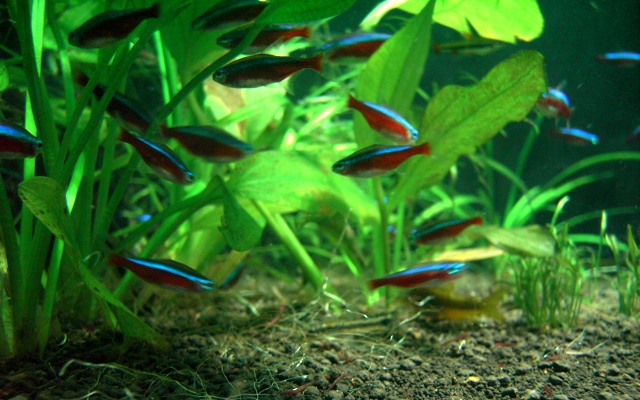
\includegraphics{neontetra}}\\
        Input image
      \end{center}
    \end{minipage}
    \begin{minipage}[c]{.14\textwidth}
      \begin{center}
        \resizebox{.8\textwidth}{!}{
\includegraphics{neon}}\medskip\\
        {\Huge\rarr}
        Reference image
      \end{center}
    \end{minipage}
    \begin{minipage}[c]{.42\textwidth}
      \begin{center}
        \resizebox{\textwidth}{!}{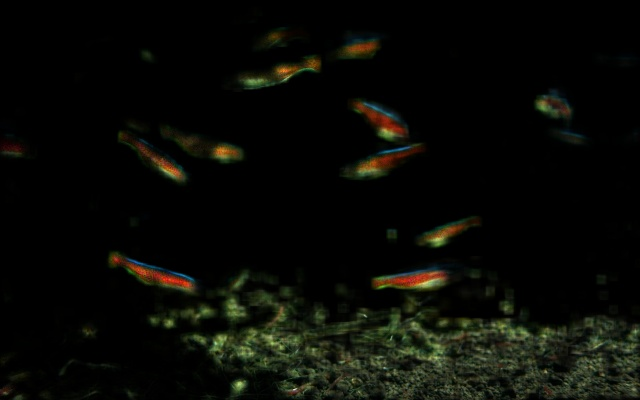
\includegraphics{fish}}\\
        Output image
      \end{center}
    \end{minipage}
    \caption{Histogram segmentation example\label{fig:fish}}
  \end{center}
\end{figure}
The input image is a picture of a tropical aquarium with Neon Tetra fish. The histogram of the reference image is used as a \ac{LUT}. The result is used to create an output image which highlights the areas which have similar colours as found in the reference image. Although the floor of the aquarium is not fully discarded, the algorithm is able to highlight most of the fish visible in the image.

The histograms of the red, green, and blue colour channels of the reference image are shown in \fig{hist}, \ie three \ac{1D} histogram.
\begin{figure}[htbp]
  \begin{center}
    \begin{tikzpicture}[ycomb,x=5pt,y=.6pt]
      \foreach \x/\xtext in {0,8,...,64}
      {
        \draw[-][color=black,very thin] (\x,0.5) -- (\x,-4.5);
        \draw[shift={(\x,-4.5)}] node[below] {\xtext};
      };
      \foreach \y/\ytext in {0,32,...,224}
      {
        \draw[-][color=gray,dashed,very thin] (-0.5,\y) -- (64.5,\y);
        \draw[shift={(-0.5,\y)}] node[left] {\ytext};
      };
      \draw[color=red!100,opacity=0.6,line width=4pt,shift={(0,0)}]
      plot coordinates{(0, 0) (1, 0) (2, 0) (3, 0) (4, 9) (5, 15) (6, 16) (7, 25) (8, 45) (9, 63) (10, 83) (11, 129) (12, 91) (13, 80) (14, 75) (15, 76) (16, 109) (17, 108) (18, 117) (19, 101) (20, 84) (21, 84) (22, 74) (23, 75) (24, 65) (25, 65) (26, 37) (27, 36) (28, 48) (29, 33) (30, 41) (31, 42) (32, 44) (33, 43) (34, 35) (35, 33) (36, 29) (37, 42) (38, 44) (39, 32) (40, 11) (41, 19) (42, 2) (43, 0) (44, 0) (45, 0) (46, 0) (47, 0) (48, 0) (49, 0) (50, 0) (51, 0) (52, 0) (53, 0) (54, 0) (55, 0) (56, 0) (57, 0) (58, 0) (59, 0) (60, 0) (61, 0) (62, 0) (63, 0)};
      \draw[color=green!100,opacity=0.6,line width=4pt,shift={(0,0)}]
      plot coordinates{(0, 0) (1, 0) (2, 0) (3, 31) (4, 144) (5, 93) (6, 89) (7, 118) (8, 102) (9, 116) (10, 129) (11, 134) (12, 89) (13, 63) (14, 51) (15, 50) (16, 44) (17, 45) (18, 41) (19, 60) (20, 69) (21, 90) (22, 59) (23, 47) (24, 49) (25, 42) (26, 20) (27, 18) (28, 19) (29, 16) (30, 10) (31, 8) (32, 19) (33, 13) (34, 12) (35, 7) (36, 10) (37, 11) (38, 15) (39, 10) (40, 12) (41, 13) (42, 10) (43, 20) (44, 16) (45, 15) (46, 18) (47, 25) (48, 18) (49, 19) (50, 18) (51, 11) (52, 7) (53, 4) (54, 3) (55, 4) (56, 3) (57, 1) (58, 0) (59, 0) (60, 0) (61, 0) (62, 0) (63, 0)};
      \draw[color=blue!100,opacity=0.6,line width=4pt,shift={(0,0)}]
      plot coordinates{(0, 3) (1, 86) (2, 196) (3, 200) (4, 245) (5, 187) (6, 139) (7, 107) (8, 94) (9, 61) (10, 96) (11, 98) (12, 57) (13, 53) (14, 23) (15, 35) (16, 18) (17, 6) (18, 6) (19, 3) (20, 3) (21, 4) (22, 9) (23, 17) (24, 12) (25, 8) (26, 3) (27, 10) (28, 4) (29, 8) (30, 2) (31, 15) (32, 7) (33, 10) (34, 7) (35, 14) (36, 6) (37, 10) (38, 3) (39, 8) (40, 1) (41, 11) (42, 3) (43, 11) (44, 8) (45, 9) (46, 5) (47, 7) (48, 6) (49, 9) (50, 1) (51, 6) (52, 4) (53, 11) (54, 7) (55, 12) (56, 5) (57, 15) (58, 5) (59, 9) (60, 15) (61, 17) (62, 18) (63, 92)};
      \draw[-][shift={(0,0)}] (-1,0) -- (65,0);
    \end{tikzpicture}
    \caption{Histograms of the red, green, and blue colour channel of the reference image\label{fig:hist}}
  \end{center}
\end{figure}
The histogram segmentation example however uses a \ac{3D} histogram which is more difficult to visualise. See \fig{hist3d} for a visualisation of the \ac{3D} histogram using a visual representation inspired by \citet{hist3d} (the visualisation was created using the POV-Ray ray tracer~\citep{RefWorks:51}).
\begin{figure}[htbp]
   \begin{center}
     \resizebox{.7\textwidth}{!}{\includegraphics{hist3d}}\\
     \caption{\acs{3D} histogram\label{fig:hist3d}}
   \end{center}
\end{figure}
Note that in practise it is often preferable to use a colour space which is independent of the luminosity (\eg \ac{HSV}).
  
\section{\acs{JIT} Compiler}\label{cha:jitcomp}
In order to achieve real-time performance, each array operation is converted to a C method on-the-fly. The C method is compiled to a Ruby extension (\ie a \ac{SO} file or a \ac{DLL}). This library is loaded dynamically and the method is registered with the Ruby \ac{VM}. Then the method is called with the appropriate parameters (also see \cha{rubyext}). The following sections explain how the C code is generated.

\subsection{Stripping Terms}
\lst{neg} shows a simple negation of an integer value. A lazy negation is instantiated explicitly to avoid immediate evaluation in Ruby.
\lstset{language=Ruby,frame=single,numbers=left}
\begin{lstlisting}[float,caption={Lazy negation of integer},escapechar=\$,label=lst:neg,name=gcc]
a = INT 5
# INT(5)
b = ElementWise(proc { |x| -x }, :-@).new a
$\textcolor{commentgray}{\# Continued in \lst{strip} ...}$
\end{lstlisting}
The equivalent in formal notation is shown in \equ{strip}.
\begin{equation}\label{equ:strip}
  a=-5\mathrm{,\ }b=-a
\end{equation}

In practise it is necessary to compute the values of every expression at some point and store the value(s) in memory. In this case it can be done by introducing the operation $store_{\acs{Z}}$ which has a side-effect on the memory location pointed to by $r$ as shown in \equ{store}.
\begin{equation}\label{equ:store}
  store_{\acs{Z}}\big(r,-a\big)
\end{equation}

\subsection{Compilation and Caching}\label{cha:caching}
In order to generate the corresponding C code, the expression of \lst{neg} is stripped as shown in \lst{strip} in line 4.
\lstset{language=Ruby,frame=single,numbers=left}
\begin{lstlisting}[float,caption={Stripping values from an expression},escapechar=\$,label=lst:strip,name=gcc]
$\textcolor{commentgray}{\# ... continuing from \lst{neg}}$
r = Pointer(INT).new
term = Store.new r, b
variables, values, skeleton = term.strip
# [[Variable(*(INT)), Variable(INT)], [*(INT)(Malloc(4)), INT(5)],
#  Store(Variable(*(INT)),-@(Variable(INT)))]
types = variables.collect { |var| var.meta }
# [*(INT), INT]
$\textcolor{commentgray}{\# Continued in \lst{descr} ...}$
\end{lstlisting}
The stripping operations results in variables, the corresponding values, and a skeleton of the expression. To avoid repeated compilation of the same expression, a unique descriptor of the expression will be used as a method names. \lst{descr} shows how the method name is computed.
\lstset{language=Ruby,frame=single,numbers=left}
\begin{lstlisting}[float,caption={Generating a unique descriptor},escapechar=\$,label=lst:descr,name=gcc]
$\textcolor{commentgray}{\# ... continuing from \lst{strip}}$
labels = Hash[*variables.zip((0 ... variables.size).to_a).flatten]
# {Variable(*(INT))=>0, Variable(INT)=>1}
descriptor = skeleton.descriptor labels
# "Store(Variable0(*(INT)),-@(Variable1(INT)))"
method_name = ('_' + descriptor).tr('(),+\-*/%.@?~&|^<=>',
                                    '0123\456789ABCDEFGH')
# "_Store0Variable0050INT112490Variable10INT111"
$\textcolor{commentgray}{\# Continued in \lst{gcc} ...}$
\end{lstlisting}
The hash table \code{labels} with labels for the variables is created (line 2) in order to distinguish expressions where only the order of variables is different. This hash table is used to generate a unique descriptor for the stripped expression (line 4). Since method names in C cannot contain special characters, a translation table is used to replace special characters with alphanumerical ones (lines 6--7).

The variables of the stripped expression are substituted with parameter objects (\ie \code{param0}, \code{param1}, $\ldots$) as shown in line 28 of \lst{gcc}.
\lstset{language=Ruby,frame=single,numbers=left}
\begin{lstlisting}[float,caption={Using special objects to generate C code},escapechar=\$,label=lst:gcc,name=gcc]
$\textcolor{commentgray}{\# ... continuing from \lst{descr}}$
c = GCCContext.new 'extension'
f = GCCFunction.new c, method_name, *types
subst = Hash[*variables.zip(f.params).flatten]
# {Variable(*(INT))=>*(INT)(param0), Variable(INT)=>INT(param1)}
skeleton.subst(subst).demand
f.compile
$\textcolor{commentgray}{\# Continued in \lst{cache} ...}$
\end{lstlisting}
This expression is re-evaluated (by calling \code{\#demand}) in order to generate C code (line 28). In this example the code for a function to compute $-a$ is generated. This is achieved using operator overloading. \Ie re-evaluating generates code instead of performing the actual computation. \lst{jit} shows the C method generated by above example.
\lstset{language=C,frame=single,numbers=none}
\begin{lstlisting}[float,caption={The resulting C code to \lst{gcc}},label=lst:jit]
VALUE _Store0Variable0050INT112490Variable10INT111(unsigned char *param0,
                                                   int param1)
{
  int v01;
  int v02;
  v01 = param1;
  v02 = -(v01);
  *(int *)(param0 + 0) = v02;
}
\end{lstlisting}
In addition code for registering the method and for converting the arguments is generated. The code is not shown here. See \lst{sitelib} for a complete listing of a Ruby extension.

The compiled code becomes a class method of the class \code{GCCCache}. \lst{cache} shows how the method is called. The arguments are extracted from the values (line 32). The C method is called and it writes the result to the specified memory location (line 34).
\lstset{language=Ruby,frame=single,numbers=left}
\begin{lstlisting}[float,caption={Calling the compiled method},escapechar=\$,label=lst:cache,name=gcc]
$\textcolor{commentgray}{\# ... continuing from \lst{gcc}}$
args = values.collect { |arg| arg.values }.flatten
# [Malloc(4), 5]
GCCCache.send method_name, *args
r
# INT(-5)
\end{lstlisting}
Note that the code is sufficiently generic to handle cases where the result of the computation is a composite number or an array.

\section{Unit Testing}
\added{The implementations of the various array operations presented in this chapter and the \ac{JIT} compiler are tested using unit testing (also see \sct{unittesting}.)} 

\added{Scalar operations can be seen as units which can be tested individually. \lst{intunit} shows a few tests for operations on boxed integers (introduced in \sct{integers}).}
\lstset{language=Ruby,frame=single,numbers=none}
\begin{lstlisting}[float=htbp,caption={Some unit tests for integers},label=lst:intunit]
require 'test/unit'
require 'multiarray'
class TC_Int < Test::Unit::TestCase
  I = Hornetseye::INT
  def I(*args)
    Hornetseye::INT *args
  end
  def test_int_inspect
    assert_equal 'INT', I.inspect
  end
  def test_typecode
    assert_equal I, I.new.typecode
  end
  def test_shape
    assert_equal [], I.new.shape
  end
  def test_inspect
    assert_equal 'INT(42)', I(42).inspect
  end
  def test_plus
    assert_equal I(3 + 5), I(3) + I(5)
  end
end
# Loaded suite irb
# Started
# .....
# Finished in 0.001675 seconds.
#
# 5 tests, 5 assertions, 0 failures, 0 errors
\end{lstlisting}

\added{Array operations are tested in a similar fashion. \lst{arrunit} shows a few tests for array operations.}
\begin{lstlisting}[float=htbp,caption={Tests for array operations},label=lst:arrunit]
require 'test/unit'
require 'multiarray'
class TC_Int < Test::Unit::TestCase
  O = Hornetseye::OBJECT
  I = Hornetseye::INT
  C = Hornetseye::INTRGB
  M = Hornetseye::MultiArray
  def S(*args)
    Hornetseye::Sequence *args
  end
  def M(*args)
    Hornetseye::MultiArray *args
  end
  def test_multiarray_inspect
    assert_equal 'MultiArray(OBJECT,2)', M(O,2).inspect
    assert_equal 'MultiArray(OBJECT,2)', S(S(O)).inspect
  end
  def test_int_inspect
    assert_equal 'INT', I.inspect
  end
  def test_typecode
    assert_equal O, M(O, 2).new(3, 2).typecode
    assert_equal I, M(I, 2).new(3, 2).typecode
    assert_equal C, M(C, 2).new(3, 2).typecode
  end
  def test_shape
    assert_equal [3, 2], M(O, 2).new(3, 2).shape
  end
  def test_inspect
    assert_equal "MultiArray(OBJECT,2):\n[[:a, 2, 3],\n  [4, 5, 6]]",
                 M[[:a, 2, 3], [4, 5, 6]].inspect
  end
  def test_plus
    assert_equal M[[2, 3, 5], [3, 5, 7]],
                 M[[1, 2, 4], [2, 4, 6]] + 1
    assert_equal M[[2, 3, 5], [3, 5, 7]],
                 1 + M[[1, 2, 4], [2, 4, 6]]
    assert_equal M[[-1, 2, 3], [4, 5, 6]],
                 M[[-3, 2, 1], [8, 6, 4]] +
                 M[[2, 0, 2], [-4, -1, 2]]
  end
  def test_dilate
    assert_equal [[1, 1, 0], [1, 1, 0], [0, 0, 0]],
                 M[[1, 0, 0], [0, 0, 0], [0, 0, -1]].dilate.to_a
  end
end
# Loaded suite irb
# Started
# .......
# Finished in 2.230944 seconds.
# 7 tests, 12 assertions, 0 failures, 0 errors
\end{lstlisting}
\added{Technically speaking these are functional tests, since the array operations are not tested separately from the scalar operations.}

\section{Summary}\label{cha:rubyvisionsum}
In this chapter a Ruby \changed{DSL}{library} for implementing machine vision algorithms was developed. A set of native basic types was introduced. It was shown that multi-dimensional, uniform arrays can be represented as lazy pointer operations. \Ie multi-dimensional arrays are just a special case of functions. Finally a generic set of operations on these data types was introduced. In some cases it was shown, how this array operations relate to image processing.

\begin{savequote}[8cm]
  \begin{singlespace}
    \underline{Seldon}: ``I have said, and I say again, that Trantor will lie in ruins within the next three centuries.''\\
    \underline{Advocate}: ``You do not consider your statement a disloyal one?''\\
    \underline{Seldon}: ``No, sir. Scientific truth is beyond loyalty and disloyalty.''\\
    \underline{Advocate}: ``You are sure that your statement represents scientific truth?''\\
    \underline{Seldon}: ``I am.''\\
    \underline{Advocate}: ``On what basis?''\\
    \underline{Seldon}: ``On the basis of the mathematics of psychohistory.''\\
    \underline{Advocate}: ``Can you prove that this mathematics is valid?''\\
    \underline{Seldon}: ``Only to another mathematician.''
    \qauthor{Isaac Asimov - The Foundation Trilogy}
  \end{singlespace}
\end{savequote}
\chapter{Input/Output}\label{cha:io}
Apart from the array operations introduced in \cha{rubyvision}, implementation of machine vision systems requires input and output of images. \fig{interfaces} gives an overview of the \ac{I}/\ac{O} integration implemented in context of this thesis. There are image sources (cameras and files) and image sinks (displays and files). Furthermore there are other popular free software libraries which were integrated in order to take advantage of the functionality offered by them (Fourier transforms) or in order to facilitate projects requiring integration of other competing projects (OpenCV, NArray).
\begin{figure}[htbp]
   \begin{center}
     \resizebox{\textwidth}{!}{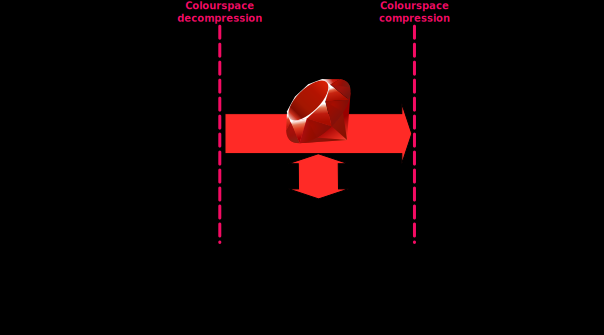
\includegraphics{interfaces}}\\
     \caption{Input/output integration\label{fig:interfaces}}
   \end{center}
\end{figure}

This chapter introduces various \ac{I}/\ac{O} libraries and how they interoperate with the array operations introduced in the previous section.
\begin{itemize}
\item \sct{csp} explains different colour spaces commonly used by \ac{I}/\ac{O} devices
\item \sct{rmagick} presents the interface to the RMagick library for loading and saving \ac{LDR} images
\item \sct{hdr} shows the integration of the OpenEXR library for loading and saving \ac{HDR} images
\item \sct{ffmpeg} covers the different issues one encounters with encoding and decoding video files
\item \sct{caminput} points out how Ruby closures can be used to provide a powerful and concise \ac{API} for accessing cameras
\item \sct{display} shows how Ruby closures can be used to implement a concise \ac{API} for displaying videos
\item The integration of an \ac{RGBD} sensor is presented in \sct{kinect} 
\item \sct{gui} is about the integration with the Qt4-QtRuby library for developing \acp{GUI}
\item \sct{sumio} gives a summary of this chapter
\end{itemize}

\section{Colour Spaces}\label{cha:csp}
\subsection{\acs{sRGB}}\label{cha:rgb}
There are different representations of images (see \tbl{image}).
\begin{table}[htbp]
  \begin{center}
    \caption{Different types of images\label{tbl:image}}\vspace{1em}
    \begin{small}
      \begin{tabular}{ll}\toprule
        \parbox[t]{.37\textwidth}{discrete, finite, quantised, grey scale function} &
        \parbox[t]{.55\textwidth}{$g\acs:\{0,1,\ldots,w-1\}\acs{TIMES}\{0,1,\ldots,h-1\}\acs{TO}\{0,1,\ldots,255\}$}\smallskip\\
        \parbox[t]{.37\textwidth}{discrete, finite, high dynamic range, grey scale function} &
        \parbox[t]{.55\textwidth}{$g:\{0,1,\ldots,w-1\}\acs{TIMES}\{0,1,\ldots,h-1\}\acs{TO}\acs{R}$}\smallskip\\
        \parbox[t]{.37\textwidth}{discrete, infinite, high dynamic range, grey scale function} &
        \parbox[t]{.55\textwidth}{$g:\acs{Z}^2\acs{TO}\acs{R}$}\smallskip\\
        \parbox[t]{.37\textwidth}{continuous, infinite, high dynamic range, grey scale function} &
        \parbox[t]{.55\textwidth}{$g:\acs{R}^2\acs{TO}\acs{R}$}\\\midrule
        \parbox[t]{.37\textwidth}{discrete, finite, quantised, colour function} &
        \parbox[t]{.55\textwidth}{$\vec{c}:\{0,1,\ldots,w-1\}\acs{TIMES}\{0,1,\ldots,h-1\}\acs{TO}\{0,1,\ldots,255\}^3$}\smallskip\\
        \parbox[t]{.37\textwidth}{discrete, finite, high dynamic range, colour function} &
        \parbox[t]{.55\textwidth}{$\vec{c}:\{0,1,\ldots,w-1\}\acs{TIMES}\{0,1,\ldots,h-1\}\acs{TO}\acs{R}^3$}\smallskip\\
        \parbox[t]{.37\textwidth}{discrete, infinite, high dynamic range, colour function} &
        \parbox[t]{.55\textwidth}{$\vec{c}:\acs{Z}^2\acs{TO}\acs{R}^3$}\smallskip\\
        \parbox[t]{.37\textwidth}{continuous, infinite, high dynamic range, colour function} &
        \parbox[t]{.55\textwidth}{$\vec{c}:\acs{R}^2\acs{TO}\acs{R}^3$}\\\bottomrule
      \end{tabular}
    \end{small}
  \end{center}
\end{table}
In practise images are discrete, finite, quantised, grey scale or colour functions. The image is acquired by a capturing device with a limited number of photosensitive cells. On the other hand for purposes of theoretical signal processing it can be beneficial to represent images as continuous, infinite, high dynamic range, colour functions. \Eg when dealing with convolutions (see \sct{convolutions}) using a finite domain would require a formal treatment of the image boundaries.

There is no upper limit for $g(\vec{x})$ which expresses the fact that there is no upper limit for luminosity \citetext{see \citealp{RefWorks:422} for a detailed introduction to high dynamic range imaging}. In practise however, most capture and display devices have a limited and quantised codomain (typically it is $\{0,1,\ldots,255\}$ or $\{0,1,\ldots,255\}^3$).

Humans have trichromatic vision. There are different colour spaces for representing trichromatic images. Usually the \ac{sRGB} is used with primaries defined in terms of the \acs{CIE} 1391 primaries~\citep{cie}. These are not as generally believed the sensitivity curves of the human photosensitive cones, which have maxima at 445 nm, 535 nm, and 570 nm~\citep{RefWorks:440} (furthermore the photo receptors for black-and-white vision at night have their sensitivity maximum at 507 nm). However as long as the sensitivity curves of the three colour channels of the camera are more or less accurate linear combinations of the sensitivity curves of the human visual cortex, it is possible to accurately reproduce the visual impression perceived by the human visual cortex.

It is worth mentioning that the relation between the radiant intensity (or luminosity) and the luma value is non-linear. The \acs{sRGB} standard closely models the behaviour of a \ac{CRT} monitor with gamma of 2.2 while avoiding a slope of zero at the origin for practical reasons. Given \ac{sRGB} values in $[0,1]$ the corresponding linear intensity values can be obtained using \equ{srgb} (where $C$ is one of \acs{red}, \acs{green}, or \acs{blue})~\citep{srgb}.
\begin{equation}\label{equ:srgb}
  C_\mathrm{linear}=
  \begin{cases}\frac{C_\mathrm{\acs{sRGB}}}{12.92}, & C_\mathrm{\acs{sRGB}}\le0.04045\\
  \left(\frac{C_\mathrm{\acs{sRGB}}+0.055}{1.055}\right)^{2.4}, & C_\mathrm{\acs{sRGB}}>0.04045
  \end{cases}
\end{equation}
Although for performance reasons it is omitted in the work presented here, strictly speaking one has to take the \acs{sRGB} definition into account when processing images. \Eg many web browsers (and even image processing programs) implicitly assume a gamma of 1.0 when scaling images which can lead to significant errors~\citep{gamma}.

\subsection{\acs{Y}\acs{Cb}\acs{Cr}}\label{cha:yuv}
Many cameras make use of compressed colour spaces. The \acs{Y}\acs{Cb}\acs{Cr} (or \acs{Y}\acs{U}\acs{V}) colour space separates luma- and colour-information as shown in \equ{yuv} (\acs{red}, \acs{green}, and \acs{blue} represent the red, green, and blue channel of an image)~\citep{fourcc}.
\begin{equation}\label{equ:yuv}
  \begin{pmatrix}\acs{Y}\\\acs{Cb}\\\acs{Cr}\end{pmatrix}=
  \begin{pmatrix}0.299&0.587&0.114\\
    -0.168736&-0.331264&0.500\\
    0.500&-0.418688&-0.081312
  \end{pmatrix}\,
  \begin{pmatrix}\acs{red}\\\acs{green}\\\acs{blue}\end{pmatrix}+
  \begin{pmatrix}0\\128\\128\end{pmatrix}
\end{equation}

The \acs{Y}\acs{Cb}\acs{Cr} colour space actually is the digital version (with values in $\{0,1,\ldots,255\}$) of the \acs{Y}\acs{Pb}\acs{Pr} colour space (see \equ{ypbpr}).
\begin{equation}\label{equ:ypbpr}
  \begin{pmatrix}\acs{Y}\\\acs{Pb}\\\acs{Pr}\end{pmatrix}=
  \begin{pmatrix}\acs{Kr}\,\acs{red}+(1-\acs{Kr}-\acs{Kb})\,\acs{green}+\acs{Kb}\,\acs{blue}\\
    \cfrac{1}{2}\,\cfrac{\acs{blue}-\acs{Y}}{1-\acs{Kb}}\\
    \cfrac{1}{2}\,\cfrac{\acs{red}-\acs{Y}}{1-\acs{Kr}}\end{pmatrix}\mathrm{,\,where\ }
  \begin{array}{c}
    \acs{red},\acs{green},\acs{blue}\in[0,1]\\
    \acs{Y}\in[0,1]\\
    \acs{Pb},\acs{Pr}\in[-0.5,0.5]
  \end{array}
\end{equation}
The values \acs{Kr} and \acs{Kb} are the estimated sensitivities of the human photo receptors for black-and-white vision to the colours red and blue. Here (\ie in \equ{yuv}) the definitions $\acs{Kr}=0.299$ and $\acs{Kb}=0.114$ of the \ac{JPEG} standard~\citep{RefWorks:441} are used (\eg see \fig{image}).
\begin{figure}[htbp]
   \begin{center}
     \begin{minipage}[c]{.495\textwidth}
       \resizebox{\textwidth}{!}{\includegraphics{fubk}}
     \end{minipage}
     \begin{minipage}[c]{.495\textwidth}
       \resizebox{\textwidth}{!}{\includegraphics{grey}}
     \end{minipage}
     \caption{Colour image and corresponding grey scale image according to sensitivities of the human eye\label{fig:image}}
   \end{center}
\end{figure}

\fig{colourspaces} gives a visual explanation of colour space compression. While the \ac{Y} channel is provided in high resolution, the chroma channels \ac{Cb} and \ac{Cr} are sampled with a lower resolution. Note that the chroma channels cannot be visualised separately. In fact chroma values can represent negative colour offsets.
\begin{figure}[htbp]
  \begin{center}
    \begin{minipage}[c]{.49\textwidth}
      \begin{center}
        \begin{tabular}{cc}
          \begin{minipage}{.46\textwidth}
            \begin{center}
              \textbf{$\acs{Y}$}\\
              \resizebox*{\textwidth}{!}{\includegraphics{y}}
            \end{center}
          \end{minipage} &
          \begin{minipage}{.46\textwidth}
            \begin{center}
              \textbf{$\acs{Y}+\acs{Cr}$}\\
              \resizebox*{\textwidth}{!}{\includegraphics{ycr}}
            \end{center}
          \end{minipage}\medskip\\
          \begin{minipage}{.46\textwidth}
            \begin{center}
              \textbf{$\acs{Y}+\acs{Cb}$}\\
              \resizebox*{\textwidth}{!}{\includegraphics{ycb}}
            \end{center}
          \end{minipage} &
          \begin{minipage}{.46\textwidth}
            \begin{center}
              \textbf{$\acs{Y}+\acs{Cb}+\acs{Cr}$}\\
              \resizebox*{\textwidth}{!}{\includegraphics{colours}}
            \end{center}
          \end{minipage}
        \end{tabular}
      \end{center}
    \end{minipage}
    \begin{minipage}[c]{.45\textwidth}
      \begin{center}
        \begin{tabular}{llc}\toprule
                & \textbf{Channel} & \textbf{Resolution}\\\midrule
          \acs{Y}  & \acl{Y}  & high\\
          \acs{Cb} & \acl{Cb} & low \\
          \acs{Cr} & \acl{Cr} & low \\\bottomrule
        \end{tabular}
      \end{center}
    \end{minipage}\\
    \caption{Colour space conversions~\citep{fourcc}\label{fig:colourspaces}}
  \end{center}
\end{figure}

\acs{Y}, \acs{Cb}, and \acs{Cr} are also known as \acs{Y}, \acs{U}, and \acs{V}. In practise there are various ways of ordering, sub sampling, and aligning the channels \citet{fourcc}. Popular pixel formats are
\begin{itemize}
\item \textbf{YV12:} The format comprises an $n\acs{TIMES} m$ \ac{Y} plane followed by $\frac{n}{2}\acs{TIMES}\frac{m}{2}$ \ac{V} and \ac{U} planes (see \fig{yv12}). The lines of each plane are 8-byte memory-aligned.
\item \textbf{I420:} Same as YV12 but the \ac{V} plane follows the \ac{U} plane.
\item \textbf{YUY2:} This is a packed pixel format. The \ac{V} and \ac{U} component are down sampled only in one direction. The component packing order is $Y_0$, $U_0$, $Y_1$, $V_0$ (see \fig{yuy2}). The lines are 8-byte memory aligned.
\item \textbf{UYVY:} Same as UYVY but with different component packing order (see \fig{uyvy}).
\end{itemize}
\begin{figure}[htbp]
  \begin{center}
    \begin{scriptsize}
      \begin{minipage}[c]{.39\textwidth}
        \begin{flushright}
          \begin{tabular}{|c|c|c|c|c|}\hline
            $Y_{0,0}$   & $Y_{1,0}$   & $\cdots$ & $Y_{n-2,0}$   & $Y_{n-1,0}$   \\\hline
            $Y_{0,1}$   & $Y_{1,1}$   & $\cdots$ & $Y_{n-2,1}$   & $Y_{n-1,1}$   \\\hline
            $\vdots$    & $\vdots$    & $\ddots$ & $\vdots$      & $\vdots$      \\\hline
            $Y_{0,m-2}$ & $Y_{1,m-2}$ & $\cdots$ & $Y_{n-2,m-2}$ & $Y_{n-1,m-2}$ \\\hline
            $Y_{0,m-1}$ & $Y_{1,m-1}$ & $\cdots$ & $Y_{n-2,m-1}$ & $Y_{n-1,m-1}$ \\\hline
          \end{tabular}
        \end{flushright}
      \end{minipage}
      \begin{minipage}[c]{.27\textwidth}
        \begin{center}
          \begin{tabular}{|c|c|c|c|c|}\hline
            \multicolumn{2}{|c|}{\multirow{2}{*}{$V_{0,0}$}} & $\cdots$ & \multicolumn{2}{|c|}{\multirow{2}{*}{$V_{n/2-1,0}$}} \\\cline{3-3}
            \multicolumn{2}{|c|}{}    & $\cdots$ & \multicolumn{2}{|c|}{} \\\hline
            $\vdots$    & $\vdots$    & $\ddots$ & $\vdots$ & $\vdots$    \\\hline
            \multicolumn{2}{|c|}{\multirow{2}{*}{$V_{0,m/2-1}$}} & $\cdots$ & \multicolumn{2}{|c|}{\multirow{2}{*}{$V_{n/2-1,m/2-1}$}} \\\cline{3-3}
            \multicolumn{2}{|c|}{}    & $\cdots$ & \multicolumn{2}{|c|}{} \\\hline
          \end{tabular}
        \end{center}
      \end{minipage}
      \begin{minipage}[c]{.27\textwidth}
        \begin{flushleft}
          \begin{tabular}{|c|c|c|c|c|}\hline
            \multicolumn{2}{|c|}{\multirow{2}{*}{$U_{0,0}$}} & $\cdots$ & \multicolumn{2}{|c|}{\multirow{2}{*}{$U_{n/2-1,0}$}} \\\cline{3-3}
            \multicolumn{2}{|c|}{}    & $\cdots$ & \multicolumn{2}{|c|}{} \\\hline
            $\vdots$    & $\vdots$    & $\ddots$ & $\vdots$ & $\vdots$    \\\hline
            \multicolumn{2}{|c|}{\multirow{2}{*}{$U_{0,m/2-1}$}} & $\cdots$ & \multicolumn{2}{|c|}{\multirow{2}{*}{$U_{n/2-1,m/2-1}$}} \\\cline{3-3}
            \multicolumn{2}{|c|}{}    & $\cdots$ & \multicolumn{2}{|c|}{} \\\hline
          \end{tabular}
        \end{flushleft}
      \end{minipage}
    \end{scriptsize}
    \caption{YV12 colour space~\citep{fourcc}\label{fig:yv12}}
  \end{center}
\end{figure}
\begin{figure}
  \begin{center}
    \begin{small}
      \begin{tabular}{|c|c|c|c||c|c|c|c||c}\hline
        $Y_{0,0}$ & $U_{0,0}$ & $Y_{1,0}$ & $V_{0,0}$ & $Y_{2,0}$ & $U_{1,0}$ & $Y_{3,0}$ & $V_{1,0}$ & $\cdots$ \\\hline
        $Y_{0,1}$ & $U_{0,1}$ & $Y_{1,1}$ & $V_{0,1}$ & $Y_{2,1}$ & $U_{1,1}$ & $Y_{3,1}$ & $V_{1,1}$ & $\cdots$ \\\hline
        $\vdots$ & $\vdots$ & $\vdots$ & $\vdots$ & $\vdots$ & $\vdots$ & $\vdots$ & $\vdots$ & $\ddots$
      \end{tabular}
    \end{small}
    \caption{YUY2 colour space~\citep{fourcc}\label{fig:yuy2}}
  \end{center}
\end{figure}
\begin{figure}
  \begin{center}
    \begin{small}
      \begin{tabular}{|c|c|c|c||c|c|c|c||c}\hline
        $U_{0,0}$ & $Y_{0,0}$ & $V_{0,0}$ & $Y_{1,0}$ & $U_{1,0}$ & $Y_{2,0}$ & $V_{1,0}$ & $Y_{3,0}$ & $\cdots$ \\\hline
        $U_{0,1}$ & $Y_{0,1}$ & $V_{0,1}$ & $Y_{1,1}$ & $U_{1,1}$ & $Y_{2,1}$ & $V_{1,1}$ & $Y_{3,1}$ & $\cdots$ \\\hline
        $\vdots$ & $\vdots$ & $\vdots$ & $\vdots$ & $\vdots$ & $\vdots$ & $\vdots$ & $\vdots$ & $\ddots$
      \end{tabular}
    \end{small}
    \caption{UYVY colour space~\citep{fourcc}\label{fig:uyvy}}
  \end{center}
\end{figure}

In order to control colour space conversions in Ruby, compressed frame data is exposed in Ruby using parametrised classes as shown in \lst{frame}.
\lstset{language=Ruby,frame=single,numbers=none}
\begin{lstlisting}[float,caption={Handling compressed colour spaces},label=lst:frame]
img = MultiArray.load_ubytergb 'test.jpg'
# MultiArray(UBYTERGB,2):
# [ [ RGB(35,38,45), RGB(45,48,55), RGB(46,50,59), RGB(46,50,59), .... ],
#   [ RGB(46,49,56), RGB(55,58,65), RGB(56,59,68), RGB(57,60,67), .... ],
#   [ RGB(46,51,57), RGB(57,60,67), RGB(57,60,67), RGB(58,61,68), .... ],
#   [ RGB(46,51,57), RGB(58,61,68), RGB(58,61,68), RGB(58,61,68), .... ],
#   [ RGB(47,50,59), RGB(58,61,70), RGB(59,62,69), RGB(59,62,69), .... ],
#   ....
frame = img.to_yv12
# Frame(YV12,320,240)(0x042caf2a)
frame.to_ubytergb
# MultiArray(UBYTERGB,2):
# [ [ RGB(33,38,45), RGB(42,47,54), RGB(45,49,59), RGB(45,49,59), .... ],
#   [ RGB(44,48,55), RGB(53,58,65), RGB(54,59,68), RGB(54,59,68), .... ],
#   [ RGB(45,49,54), RGB(54,59,63), RGB(54,59,66), RGB(55,60,67), .... ],
#   [ RGB(45,49,54), RGB(55,60,65), RGB(55,60,67), RGB(55,60,67), .... ],
#   [ RGB(45,49,56), RGB(55,60,67), RGB(56,61,68), RGB(56,61,68), .... ],
#   ....
\end{lstlisting}
The actual conversions are performed using the FFmpeg rescaling library (libswscale). One can see that a conversion round trip from unsigned byte \ac{RGB} to YV12 and back affects the values. \fig{swscale} shows how YV12 colour space compression leads to compression artefacts when the edges do not align favourably with the lower resolution of the \ac{U} and \ac{V} channels.
\begin{figure}[htbp]
  \begin{center}
    \begin{minipage}[t]{.45\textwidth}
      \begin{center}
        \resizebox{\textwidth}{!}{\includegraphics{rgb}}\\
        original \acs{RGB} data
      \end{center}
    \end{minipage}
    \hspace{.5cm}
    \begin{minipage}[t]{.45\textwidth}
      \begin{center}
        \resizebox{\textwidth}{!}{\includegraphics{yv12}}\\
        converted to YV12 and back
      \end{center}
    \end{minipage}
    \caption{Artefacts caused by colour space compression\label{fig:swscale}}
  \end{center}
\end{figure}

\section{Image Files}\label{cha:rmagick}
The RMagick\footnote{\url{http://rmagick.rubyforge.org/}} Ruby-extension allows one to use the powerful ImageMagick/Magick++\footnote{\url{http://www.imagemagick.org/Magick++/}} library in Ruby for loading and saving images. The ImageMagick library supports a large number of file formats. Frequently used file formats are
\begin{itemize}
\item \acf{BMP} format
\item \acf{GIF}
\item \acf{PNG} format
\item \acf{PPM} format (with variations \acf{PGM} and \acf{PBM})
\item \acf{JPEG} format
\item \acf{TIFF}
\item \acf{DICOM}
\end{itemize}
In general one needs a format for lossy compression (\eg \ac{JPEG}) and a format for lossless compression (\eg \ac{PNG}) when using 8-bit grey scale or 24-bit colour images (\eg see \fig{lossy}).
\begin{figure}[htbp]
   \begin{center}
     \begin{minipage}[c]{.495\textwidth}
       \resizebox{\textwidth}{!}{\includegraphics{lossless}}
     \end{minipage}
     \begin{minipage}[c]{.495\textwidth}
       \resizebox{\textwidth}{!}{\includegraphics{lossy}}
     \end{minipage}
     \caption{Low resolution colour image using lossless \acs{PNG} and (extremely) lossy \acs{JPEG} compression\label{fig:lossy}}
   \end{center}
\end{figure}
\lst{loadsave} shows how the functionality of the RMagick Ruby-extension was integrated.
\lstset{language=Ruby,frame=single,numbers=none}
\begin{lstlisting}[float,caption={Loading and saving images},label=lst:loadsave]
img = MultiArray.load_ubytergb 'lossless.png'
# MultiArray(UBYTERGB,2):
# [ [ RGB(18,14,13), RGB(21,15,15), RGB(24,17,14), RGB(27,19,14), .... ],
#   [ RGB(34,20,14), RGB(36,18,14), RGB(78,51,34), RGB(88,63,43), .... ],
#   [ RGB(33,24,18), RGB(37,23,18), RGB(69,44,23), RGB(71,40,30), .... ],
#   [ RGB(29,21,16), RGB(41,27,18), RGB(58,29,18), RGB(52,30,19), .... ],
#   [ RGB(17,11,13), RGB(37,16,17), RGB(59,24,18), RGB(43,22,17), .... ],
#   [ RGB(19,12,15), RGB(40,15,18), RGB(57,22,19), RGB(13,11,12), .... ],
#   [ RGB(20,13,15), RGB(35,15,15), RGB(44,19,17), RGB(17,12,12), .... ],
#   [ RGB(17,12,14), RGB(46,17,19), RGB(63,19,20), RGB(70,22,22), .... ],
#   [ RGB(23,13,16), RGB(64,24,21), RGB(71,31,23), RGB(79,36,26), .... ],
#   [ RGB(35,25,27), RGB(60,40,35), RGB(68,45,35), RGB(83,66,54), .... ],
#   ....
img.save_ubytergb 'lossy.jpg'
#   ....
\end{lstlisting}
The method \code{MultiArray.load\_ubytergb} uses the RMagick library to load an image and convert it to unsigned byte (8 bit) \ac{RGB} data. The resulting \code{Malloc} object (see \cha{malloc}) is used to construct a uniform array of \ac{RGB} values. The \code{\#save\_ubytergb} method provides saving unsigned byte \ac{RGB} data.

Medical image processing software frequently uses the \ac{DICOM} format for storing 16-bit radiology images and in material science \ac{TIFF} is a common format for exchanging 16-bit electron images. \fig{mono16} shows examples of images in medical science and material science. Here they are shown using 8-bit quantisation only since most computer displays do not support more than $2^8$ grey levels.
\begin{figure}[htbp]
   \begin{center}
     \begin{minipage}[t]{.495\textwidth}
       \resizebox{\textwidth}{!}{\includegraphics{mr-knee}}
         \acs{MR} scan of knee (source: \href{http://www.barre.nom.fr/medical/samples/}{Sébastien Barré's DICOM collection})
     \end{minipage}
     \begin{minipage}[t]{.495\textwidth}
       \resizebox{\textwidth}{!}{\includegraphics{tilt00}}
       \acs{TEM} image of tungsten tip (courtesy of \href{http://nano.group.shef.ac.uk/}{Sheffield University Nanorobotics Research Group})
     \end{minipage}
     \caption{Examples of images in medical science and material science\label{fig:mono16}}
   \end{center}
\end{figure}
To support saving and loading of grey scale and colour images of different depth the methods shown in \tbl{magick} were implemented (using the RMagick library).
\begin{table}[htbp]
  \begin{center}
    \caption{Methods for loading and saving images\label{tbl:magick}}\vspace{1em}
    \begin{tabular}{lll}\toprule
      \textbf{(integer) type} & \multicolumn{1}{c}{\textbf{loading}} & \multicolumn{1}{c}{\textbf{saving}}\\\midrule
      \emph{8 bit monochrome}  & \code{MultiArray.load\_ubyte} & \code{Node\#save\_ubyte}\\
      \emph{16 bit monochrome} & \code{MultiArray.load\_usint} & \code{Node\#save\_usint}\\
      \emph{32 bit monochrome} & \code{MultiArray.load\_uint}  & \code{Node\#save\_uint}\\\midrule
      \emph{8 bit \acs{RGB}}   & \code{MultiArray.load\_ubytergb} & \code{Node\#save\_ubytergb}\\
      \emph{16 bit \acs{RGB}}  & \code{MultiArray.load\_usintrgb} & \code{Node\#save\_usintrgb}\\
      \emph{32 bit \acs{RGB}}  & \code{MultiArray.load\_uintrgb}  & \code{Node\#save\_uintrgb}\\\bottomrule
    \end{tabular}
  \end{center}
\end{table}

In some cases it might be desirable to let the file format determine the image type (bit depth, grey-scale/colour) and vice versa instead of forcing it. For this case methods named \code{MultiArray.load\_magick} and \code{Node\#save\_magick} were implemented which make use of dynamic typing available in the Ruby language. In fact this two methods are the basis for the other methods for loading and saving images.

Note that dynamic typing has a compelling advantage in the case of loading images. C/C++ libraries such as OpenCV and ImageMagick cannot make use of the (static) type system of the programming language to handle image types because in general it is not desirable having to specify the image type before loading the image.

\section{\acs{HDR} Image Files}\label{cha:hdr}
Theoretically there is no upper limit for the radiant intensity. Therefore in many situation the linear quantisation (\acl{LDR}) does not allow for an optimal trade-off between quantisation noise and measurement range. The human eye uses photo receptors with different sensitivities and a non-linear response to address this problem.

It is possible to acquire \ac{HDR} images using \ac{LDR} devices with the help of exposure bracketing. \Ie a series of pictures with different exposures is acquired and fused using an algorithm. \ac{HDR} images are usually represented using arrays of floating point numbers. A popular format for \ac{HDR} images is the OpenEXR\footnote{\url{http://www.openexr.com/}} format by Industrial Light \& Magic~\citep{openexr}. The format uses 16 bit (half precision) floating point numbers.

Tone mapping is the digital analogy to the traditional technique of dodging and burning. Tone mapping maps a \ac{HDR} image to an \ac{LDR} image by locally adapting the luminosity of the image. \fig{hdr} illustrates the complete process of \ac{HDR} imaging using a consumer camera.
First a set of images with different exposures is acquired. If the camera has shifted, the images need to be aligned using feature matching (here the panorama stitching software Hugin\footnote{see \url{http://hugin.sourceforge.net/}} was used). The images are fused to an \ac{HDR} image. For display on a low dynamic range device, the image is tone mapped (here the tone mapping software QtPfsGui\footnote{see \url{http://qtpfsgui.sourceforge.net/}} was used). There are different algorithms for tone mapping. \fig{hdr} shows a result obtained using the algorithm by \citet{fattal2002gradient}.
\begin{figure}[htbp]
  \begin{center}
    \begin{minipage}[c]{.288\textwidth}
      \begin{center}
        \textbf{Exposure bracketing}\\
        \resizebox{.45\textwidth}{!}{\includegraphics{smallaudi0}}
        \resizebox{.45\textwidth}{!}{\includegraphics{smallaudi1}}\\
        \resizebox{.45\textwidth}{!}{\includegraphics{smallaudi2}}
        \resizebox{.45\textwidth}{!}{\includegraphics{smallaudi3}}\\
        \resizebox{.45\textwidth}{!}{\includegraphics{smallaudi4}}
        \resizebox{.45\textwidth}{!}{\includegraphics{smallaudi5}}\\
        \resizebox{.45\textwidth}{!}{\includegraphics{smallaudi6}}
        \resizebox{.45\textwidth}{!}{\includegraphics{smallaudi7}}\\
        \resizebox{.45\textwidth}{!}{\includegraphics{smallaudi8}}
        \resizebox{.45\textwidth}{!}{\includegraphics{smallaudi9}}
      \end{center}
    \end{minipage}
    \begin{minipage}[c]{12pt}
      \huge\farr
    \end{minipage}
    \begin{minipage}[c]{.288\textwidth}
      \begin{center}
        \textbf{Alignment (\href{http://hugin.sourceforge.net/}{Hugin})}\\
        \resizebox{.45\textwidth}{!}{\includegraphics{alignedaudi0}}
        \resizebox{.45\textwidth}{!}{\includegraphics{alignedaudi1}}\\
        \resizebox{.45\textwidth}{!}{\includegraphics{alignedaudi2}}
        \resizebox{.45\textwidth}{!}{\includegraphics{alignedaudi3}}\\
        \resizebox{.45\textwidth}{!}{\includegraphics{alignedaudi4}}
        \resizebox{.45\textwidth}{!}{\includegraphics{alignedaudi5}}\\
        \resizebox{.45\textwidth}{!}{\includegraphics{alignedaudi6}}
        \resizebox{.45\textwidth}{!}{\includegraphics{alignedaudi7}}\\
        \resizebox{.45\textwidth}{!}{\includegraphics{alignedaudi8}}
        \resizebox{.45\textwidth}{!}{\includegraphics{alignedaudi9}}
      \end{center}
    \end{minipage}
    \begin{minipage}[c]{12pt}
      \huge\farr
    \end{minipage}
    \begin{minipage}[c]{.33\textwidth}
      \begin{center}
        \textbf{\acs{HDR} compilation and tone mapping (\href{http://qtpfsgui.sourceforge.net/}{QtPfsGui})}\\
        \resizebox{\textwidth}{!}{\includegraphics{exraudi}}
      \end{center}
    \end{minipage}
    \caption{Bracketing, alignment, and tone mapping\label{fig:hdr}}
  \end{center}
\end{figure}

To support saving and loading of grey scale and colour images and convert them to floating point arrays of different depth the methods shown in \tbl{openexr} were implemented (using the OpenEXR library).
\begin{table}[htbp]
  \begin{center}
    \caption{Methods for loading and saving images\label{tbl:openexr}}\vspace{1em}
    \begin{tabular}{lll}\toprule
      \textbf{(floating point) type} & \multicolumn{1}{c}{\textbf{loading}} & \multicolumn{1}{c}{\textbf{saving}}\\\midrule
      \emph{32 bit monochr.} & \code{MultiArray.load\_sfloat} & \code{Node\#save\_sfloat}\\
      \emph{64 bit monochr.} & \code{MultiArray.load\_dfloat} & \code{Node\#save\_dfloat}\\\midrule
      \emph{32 bit \acs{RGB}}      & \code{MultiArray.load\_sfloatrgb} & \code{Node\#save\_sfloatrgb}\\
      \emph{64 bit \acs{RGB}}      & \code{MultiArray.load\_dfloatrgb} & \code{Node\#save\_dfloatrgb}\\\bottomrule
    \end{tabular}
  \end{center}
\end{table}
\lst{hdr} shows how the methods might be used in practise.
\lstset{language=Ruby,frame=single,numbers=none}
\begin{lstlisting}[float,caption={Converting an \acs{HDR} image to an \acs{LDR} image (no tone mapping)},label=lst:hdr]
img = MultiArray.load_dfloatrgb 'hdr.exr'
# ...
(img * 1000).round / 1000
# MultiArray(DFLOATRGB,2):
# [ [ RGB(0.249,0.283,0.363), RGB(0.294,0.324,0.422), .... ],
#   [ RGB(0.293,0.329,0.412), RGB(0.339,0.376,0.478), .... ],
#   [ RGB(0.289,0.337,0.429), RGB(0.345,0.389,0.486), .... ],
#   [ RGB(0.298,0.336,0.437), RGB(0.357,0.393,0.506), .... ],
#   [ RGB(0.307,0.331,0.435), RGB(0.372,0.39,0.513), .... ],
#   [ RGB(0.317,0.338,0.478), RGB(0.369,0.397,0.529), .... ],
#   [ RGB(0.324,0.34,0.514), RGB(0.362,0.4,0.548), .... ],
#   [ RGB(0.318,0.338,0.458), RGB(0.359,0.394,0.537), .... ],
#   [ RGB(0.321,0.339,0.473), RGB(0.353,0.403,0.554), .... ],
#   [ RGB(0.309,0.35,0.45), RGB(0.363,0.412,0.528), .... ],
#   ....
peak = img.max
# RGB(71.2704849243164,56.86302947998047,81.38863372802734)
factor = 255 / [peak.r, peak.g, peak.b].max
# 3.133115624622988
(img * factor).save_ubytergb 'ldr.png'
# ...
\end{lstlisting}

% capitalize table, figure, ...

Similar as in \cha{rmagick} the methods \code{MultiArray.load\_openexr} as well as the method \code{Node\#save\_openexr} let the file format determine the image type.

\section{Video Files}\label{cha:ffmpeg}
File formats generally use algorithms such as Huffmann coding for lossless compression. Image file formats furthermore exploit spatial similarity. \Eg the \ac{JPEG} format uses a block-wise discrete cosine transform followed by application of a custom quantisation matrix. Most video codecs additionally exploit temporal similarity by replacing full frames with motion vector fields and motion-compensated difference pictures. The occasional full frame is included to reduce the computational cost of randomly accessing a frame in the video.

For reading and writing video files the FFmpeg\footnote{\url{http://www.ffmpeg.org/}} library was integrated. Many video formats consist of a container format which usually offers a video stream and potentially an audio stream. Many container formats support several video and audio codecs. The video and audio codec determine the format of the video and audio stream. Popular file formats and codecs are
\begin{itemize}
\item \textbf{popular container formats}
  \begin{itemize}
  \item \acf{AVI}
  \item \acf{ASF}
  \item \acf{FLV}
  \item \acf{MOV}
  \item \acf{MPEG-4}
  \item \acf{Ogg}
  \end{itemize}
\item \textbf{popular video codecs}
  \begin{itemize}
  \item \acf{VP6}
  \item \acf{H.264}
  \item \acf{WMV}
  \item \acf{Theora}
  \end{itemize}
\item \textbf{popular audio codecs}
  \begin{itemize}
  \item \acf{AAC}
  \item \acf{MP3}
  \item \acf{Vorbis}
  \item \acf{WMA}
  \end{itemize}
\end{itemize}

\fig{decoder} shows the coarse architecture of the FFmpeg decoder. The demuxer of the container format decodes the file and generates audio and video packets. The video decoder accepts video packets and decodes video frames. The audio decoder accepts audio packets and returns audio frames. The video frames are usually given as YV12 data (see \cha{yuv}). Typically the video is given with a frame rate of 25 frames/second. Note that video data might have a pixel aspect ratio other than $1:1$ and it can be interlaced. The audio frames are given as 16-bit signed integer arrays (for stereo audio the values come in pairs of two). A common sampling rate is \unit[44.1]{kHz}.
\begin{figure}[htbp]
  \begin{center}
    \resizebox{.9\textwidth}{!}{\includegraphics{decoder}}
    \caption{Decoding videos using FFmpeg\label{fig:decoder}}
  \end{center}
\end{figure}
The audio and video frames are tagged with a presentation time stamp. The time stamps are required to synchronize the audio and video frames properly. Another reason for the existence of time stamps are video formats with support for variable frame rate.

\lst{avinput} demonstrates the behaviour of the class \code{AVInput} which was developed to make the FFmpeg decoder accessible in Ruby.
\lstset{language=Ruby,frame=single,numbers=left}
\begin{lstlisting}[float,caption={Reading a video file},label=lst:avinput]
input = AVInput.new 'test.avi'
input.frame_rate 
# (15/1)
input.sample_rate 
# 44100
input.pos = 60
input.read_video
# Frame(YV12,320,240)(0x04abdce6)
input.read_audio
# MultiArray(SINT,2):
# [ [ 0, 0 ],
#   [ 0, 0 ],
#   [ 0, 0 ],
#   [ 0, 0 ],
#   [ 0, 0 ],
#   ....
input.video_pos
# (184/3)
input.audio_pos
# (122671/2000)
\end{lstlisting}
A video file is opened (line 1) and the decoding of the first 60 seconds is skipped (line 6). A video frame ($320\acs{TIMES} 240$ YV12 data) and an audio frame (1152 16-bit stereo samples) are decoded (lines 7 and 9). At the end the time stamps of the previously decoded frames are retrieved (lines 17 and 19). One can see that the time stamps of audio and video frames do not necessarily coincide ($\frac{184}{3}=61.\bar{3}$, $\frac{122671}{2000}=61.3355$).

The FFmpeg library also supports video and audio encoding. One can see in \fig{encoder} that the encoder's data flow is symmetric to the decoder's data flow. Instead of video and audio decoders there are video and audio encoders. The demuxer is replaced with a muxer.

The class \code{AVOutput} was implemented to expose the encoding functionality of the FFmpeg library in Ruby. \lst{avoutput} shows a small program creating an MPEG-4 file with a static picture (loaded in line 5) as video and a \unit[400]{Hz} sine wave (created in lines 13--15) as audio.
\begin{figure}[htbp]
  \begin{center}
    \resizebox{.9\textwidth}{!}{\includegraphics{encoder}}
    \caption{Encoding videos using FFmpeg\label{fig:encoder}}
  \end{center}
\end{figure}
\lstset{language=Ruby,frame=single,numbers=left}
\begin{lstlisting}[float,caption={Writing a video file},label=lst:avoutput]
VIDEO_BITRATE = 500_000; AUDIO_BITRATE = 30_000
DURATION      =       3; RATE          = 44_100
FPS           =      25; CHANNELS      =      2
ASPECT        = 1.quo 1; LEN           =    110
img = MultiArray.load_ubytergb 'test.png'
# MultiArray(UBYTERGB,2):
# [ [ RGB(77,77,77), RGB(77,77,77), RGB(77,77,77), RGB(77,77,77), .... ],
#   [ RGB(77,77,77), RGB(77,77,77), RGB(77,77,77), RGB(77,77,77), .... ],
#   [ RGB(77,77,77), RGB(77,77,77), RGB(77,77,77), RGB(77,77,77), .... ],
#   [ RGB(255,255,255), RGB(255,255,255), RGB(255,255,255), .... ],
#   [ RGB(77,77,77), RGB(77,77,77), RGB(77,77,77), RGB(77,77,77), .... ],
#   ....
wave = lazy(CHANNELS, LEN) do |j,i|
  Math.sin(i * 2 * Math::PI / LEN) * 0x7FFF
end.to_sint
# MultiArray(SINT,2):
# [ [ 0, 0 ],
#   [ 1870, 1870 ],
#   [ 3735, 3735 ],
#   [ 5587, 5587 ],
#   [ 7421, 7421 ],
#   ....
output = AVOutput.new 'test.mp4', VIDEO_BITRATE, img.width, img.height,
                      FPS, ASPECT, AVOutput::CODEC_ID_MPEG4, true,
                      AUDIO_BITRATE, RATE, CHANNELS, AVOutput::CODEC_ID_MP3
(RATE * DURATION / LEN).times do
  output.write_audio wave
end
(FPS * DURATION).times do
  output.write_video img
end
\end{lstlisting}
The interface is minimalistic and does not give access to the various parameters of the encoding algorithms. When encoding a video file one has to merely specify the following basic properties (see lines 23--25 of \lst{avoutput})
\begin{itemize}
\item \textbf{video bit rate:} the approximate number of bits per second for encoding the video stream
\item \textbf{width:} the width of each video frame
\item \textbf{height:} the height of each video frame
\item \textbf{frame rate:} the number of video frames per second
\item \textbf{pixel aspect ratio:} the ratio of pixel width to pixel height
\item \textbf{video codec:} the video codec to use
\item \textbf{audio bit rate:} the approximate number of bits per second for encoding the audio stream
\item \textbf{audio sampling rate:} the number of audio samples per second
\item \textbf{audio channels:} the number of audio channels (\eg two for stereo audio)
\item \textbf{audio codec:} the audio codec to use
\end{itemize}
Note that the program shown in \lst{avoutput} encodes all the audio frames (lines 26--28) before starting to encode the video frames (lines 29--31). When creating large files this is not good practise because the muxer needs to interleave video and audio packets. \Ie the muxer would be forced to allocate a lot of memory for queueing the audio frames.

\section{Camera Input}\label{cha:caminput}
Camera input is a prime example for the benefit of closures. Initialising a camera (\eg Logitech Quickcam Pro 9000 shown in \fig{quickcam}) requires the calling program to choose a video mode (\ie width, height, and colour space).
\begin{figure}[htbp]
  \begin{center}
    \resizebox{.6\textwidth}{!}{\includegraphics{quickcam}}
    \caption{Logitech Quickcam Pro 9000 (a USB webcam)\label{fig:quickcam}}
  \end{center}
\end{figure}
However the supported video modes can only be requested \emph{after} opening the camera device. For this reasons most \acp{API} either allow the calling program to handle a camera device which is not fully initialised yet, or the calling program has to specify a preferred video mode which might not be supported by the camera.

Using closures however it is possible to involve the calling program during initialisation in an elegant way as demonstrated in \lst{v4l2select}.
\lstset{language=Ruby,frame=single,numbers=none}
\begin{lstlisting}[float,caption={Opening a V4L2 device and negotiating a video mode},label=lst:v4l2select]
camera = V4L2Input.new '/dev/video0' do |modes|
  modes.each_with_index { |mode,i| puts "#{i + 1}: #{mode}" }
  modes[STDIN.readline.to_i - 1]
end
# 1: Frame(YUY2,160,120)
# 2: Frame(YUY2,176,144)
# 3: Frame(YUY2,320,240)
# 4: Frame(YUY2,352,288)
# 5: Frame(YUY2,640,480)
# 6: Frame(YUY2,800,600)
# 7: Frame(YUY2,960,720)
# 8: Frame(YUY2,1600,1200)
# $ 6
# #<Hornetseye::V4L2Input:0x993af7c>
camera.read
# Frame(YUY2,800,600)(0x049c3d40)
\end{lstlisting}
The constructor \code{V4L2Input.new} opens the specified device (here \code{'/dev/video0'}). The supported video modes are requested, compiled to a list, and passed to the closure as a parameter. In this example the closure prints the list to the terminal and the user is prompted to select one.

\lst{v4l2fixed} gives a more minimalistic example.
\begin{lstlisting}[float,caption={Opening a V4L2 device and selecting a fixed mode},label=lst:v4l2fixed]
camera = V4L2Input.new('/dev/video0') { Frame(YUY2, 800, 600) }
# #<Hornetseye::V4L2Input:0x8ca9ee8>
camera.read
# Frame(YUY2,800,600)(0x046283d4)
\end{lstlisting}
Here it is assumed that the camera supports the specified video mode ($800\acs{TIMES} 600$, YUY2 colour space). The closure ignores the list of modes and just returns the desired resolution. If the camera does not support the desired video mode, the initialisation will fail.

\section{Image Display}\label{cha:display}
When developing computer vision algorithms it is important to be able to visually inspect processed or annotated images on the desktop. \fig{x11} shows the structure of a standard X Window desktop.
\begin{figure}[htbp]
  \begin{center}
    \framebox{\resizebox{.9\textwidth}{!}{\includegraphics{x11}}}
    \caption{Display, windows, and visuals on a standard X Window desktop\label{fig:x11}}
  \end{center}
\end{figure}
The X library allows a program to access multiple displays and open multiple windows on each of them. The window manager software draws the title bar and the window boundary. The program is only responsible for drawing the content of each window. When the program is idle it can query the X Server to get notified when an event occurs (\eg a window close button was pressed, a key was pressed, or an area of a window needs repainting).

Functionality for displaying a single image was exposed in Ruby using the \code{\#show} method as demonstrated in \lst{show1}. The method opens a window showing the image and it returns control to the calling program when the window is closed (or [Esc] or [Space] was pressed).
\lstset{language=Ruby,frame=single,numbers=none}
\begin{lstlisting}[float,caption={Loading and displaying an image},label=lst:show1]
MultiArray.load_ubytergb('test.png').show
\end{lstlisting}

Apart from displaying single images it is also important to be able to display videos. The OpenCV computer vision library offers functionality for displaying videos as shown in \lst{pycv}. The program reads frames from a video file, converts them to grey scale, and then displays them in a window.
\lstset{language=Python,frame=single,numbers=none}
\begin{lstlisting}[float,caption={Displaying a video using Python and OpenCV},label=lst:pycv]
import sys
from opencv import cv
from opencv import highgui
highgui.cvNamedWindow('test video')
capture = highgui.cvCreateFileCapture('test.avi')
while 1:
  frame = highgui.cvQueryFrame(capture)
  gray = cv.cvCreateImage(cv.cvSize(frame.width, frame.height), 8, 1)
  cv.cvCvtColor(frame, gray, cv.CV_BGR2GRAY)
  highgui.cvShowImage('test video', gray)
  if highgui.cvWaitKey(5) > 0:
    break
\end{lstlisting}

\lst{show2} shows an equivalent program implemented using Ruby and the Hornetseye Ruby extension presented in this thesis. For comparison with \lst{pycv} the complete code with loading of libraries and name space handling is given.
\lstset{language=Ruby,frame=single,numbers=none}
\begin{lstlisting}[float,caption={Displaying a video using Ruby and Hornetseye},label=lst:show2]
require 'rubygems'
require 'hornetseye_ffmpeg'
require 'hornetseye_xorg'
include Hornetseye
video = AVInput.new 'test.avi'
X11Display.show(:title => 'test video') do
  video.read.to_ubyte
end
\end{lstlisting}
The Ruby programming language has mature support for closures (see \cha{closures}). This makes it possible to implement a method such as \code{X11Display.show} which accepts a closure returning successive video frames for display. Only the custom part of the display loop needs to be specified by the calling program. Thus the calling program is much more concise and the overall redundancy is less.

\lst{show3} is another example emphasizing the importance of closures. It shows a minimalistic video player (no sound, assuming pixel aspect ratio of $1:1$, no handling of variable frame rate).
\lstset{language=Ruby,frame=single,numbers=none}
\begin{lstlisting}[float,caption={Minimalistic video player},label=lst:show3]
video = AVInput.new 'test.avi'
X11Display.show(:frame_rate => video.frame_rate) { video.read }
\end{lstlisting}
Without closures the code for synchronising video display with the clock would have to be part of the calling program. The program shown in \lst{show3} does not do any signal processing. However it provides the video \ac{I}/\ac{O} necessary to implement a machine vision algorithm with visualisation. \Ie the code of the minimalistic video player represents a lower bound for the most concise implementation of a machine vision algorithm. Therefore it is worthwhile to minimise its size.

When visualising real-time machine vision algorithms, the time for displaying the results can exceed the time of the algorithms involved. In order to address this problem one can use \ac{2D} hardware acceleration. Most graphic cards provide hardware accelerated display (the XVideo extension of the X Window System) for a single visual. The acceleration typically requires the image to be compressed as YV12 data. \lst{show4} shows how Ruby optional parameters are used to expose that functionality in Ruby.
\lstset{language=Ruby,frame=single,numbers=none}
\begin{lstlisting}[float,caption={Hardware accelerated video output},label=lst:show4]
video = AVInput.new 'test.avi'
X11Display.show(:frame_rate => video.frame_rate,
                :output => XVideoOutput) { video.read }
\end{lstlisting}
Note that adding sound \ac{I}/\ac{O} to this program results in a video player which compares with professional video player software in terms of performance (see \anx{player}).

\section{\acs{RGBD} Sensor}\label{cha:kinect}
\changed{A more recent input device is the Microsoft Kinect. The device uses an \ac{IR} laser to project a pattern.}{\ac{RGBD} sensors provide a depth channel in addition to the \ac{RGB} channels. A recent example is the Primesense sensor (which is part of the Microsoft Kinect device). The sensor uses an \ac{IR} laser to project a pattern.} The \ac{IR} camera takes a picture of the pattern and the device uses correlation techniques to estimate the disparity and the depth~\citep{primesense}. \changed{The device also comes with an \ac{RGB} camera for acquiring optical images.}{A separate \ac{RGB} camera is used to acquire optical images.} \fig{kinect} shows a depth image and optical image acquired with the device.
\begin{figure}[htbp]
  \begin{center}
    \resizebox{\textwidth}{!}{\includegraphics{kinect}}
    \caption{RGB- and depth-image acquired with an \acs{RGBD} sensor\label{fig:kinect}}
  \end{center}
\end{figure}
The image pair was acquired using the program shown in \lst{kinect}.
\lstset{language=Ruby,frame=single,numbers=none}
\begin{lstlisting}[float,caption={Ruby example for accessing a Kinect sensor},label=lst:kinect]
class Numeric
  def clip(range)
    [[self, range.begin].max, range.end].min
  end
end
colours = Sequence.ubytergb 256
for i in 0 ... 256
  hue = 240 - i * 240.0 / 256.0
  colours[i] =
    RGB(((hue - 180).abs -  60).clip(0 ...60) * 0xFF / 60.0,
        (120 - (hue - 120).abs).clip(0 ...60) * 0xFF / 60.0,
        (120 - (hue - 240).abs).clip(0 ...60) * 0xFF / 60.0)
end
input = KinectInput.new
img = MultiArray.ubytergb 1280, 480
X11Display.show do
  img[  0 ...  640, 0 ... 480] = input.read_video
  img[640 ... 1280, 0 ... 480] = (input.read_depth >> 2).clip.lut colours
  img
end
\end{lstlisting}
The Ruby bindings are based on the libfreenect library\footnote{\url{http://openkinect.org/}}. The 11-bit depth image is shifted right by 2 bits. The resulting 9-bit depth image is clipped to 8-bit values and converted to a pseudo colour image. Note that the depth image and the RGB image are not aligned properly. \Ie it is necessary to calibrate the sensor and rectify the data if depth- and RGB-images are to be used in conjunction. Another problem is that the depth- and RGB-images are always taken at different times.

\section{\acs{GUI} Integration}\label{cha:gui}
When developing a \ac{GUI} to parametrise and run computer vision algorithms it usually requires video display as part of the interface. For the work presented in this thesis the Qt4 library~\citep{qt4white} was used. The Qt4 library has become the tool of choice for developing cross-platform \acp{GUI}~\citep{qt4}. Qt4 is a C++ library. However Richard Dale's qt4-qtruby\footnote{http://rubyforge.org/projects/korundum/} extension facilitates development of \acp{GUI} in Ruby using the work flow shown in \fig{rbuic}.
\begin{figure}[htbp]
  \begin{center}
    \resizebox{.9\textwidth}{!}{\includegraphics{rbuic}}
    \caption{Work flow for creating Qt4 user interfaces\label{fig:rbuic}}
  \end{center}
\end{figure}
For displaying videos in a Qt4 \ac{GUI}, a widget for \ac{2D} hardware accelerated display (XVideo) was developed. The widget makes it possible to display videos with high frame rate as part of a \ac{GUI}. \fig{xvwidget} shows a minimalistic video player window consisting of a XVideo widget and a slider.
\begin{figure}[htbp]
  \begin{center}
    \resizebox{.6\textwidth}{!}{\includegraphics{xvwidget}}
    \caption{XVideo widget embedded in a \acs{GUI}\label{fig:xvwidget}}
  \end{center}
\end{figure}

\section{Summary}\label{cha:sumio}
In this chapter it was shown how various \ac{I}/\ac{O} facilities can be integrated into the Ruby language in order to acquire and output or store images. In order to get per-pixel access to the data, it is necessary to understand and manage colour space transformations. It was pointed out that most devices and file formats provide a limited quantisation range. However there are specific file formats (and even devices) for handling \ac{HDR} data.

Ruby closures where used to implement an \ac{API} which supports negotiation of a camera resolution when opening a camera. Ruby closures also proved to be useful for defining a concise \ac{API} for displaying videos. Furthermore the power of Ruby as a glue language comes into play when integrating the different \acp{API} for the \ac{GUI}, the video \ac{I}/\ac{O}, and image processing.

\begin{savequote}[8cm]
  \begin{singlespace}
    ``An older and by now well-accepted idea is that of the stored-program computer. In such a computer the program and the data reside in the same memory; that is, the program is itself data which can be manipulated as any other data by the processor. It is this idea which allows the implementation of such powerful and incestuous software as program editors, compilers, interpreters, linking loaders, debugging systems, etc.
    
    One of the great failings of most high-level languages is that they have abandoned this idea. It is extremely difficult, for example, for a PL/I (PASCAL, FORTRAN, COBOL ...) program to manipulate PL/I (PASCAL, FORTRAN, COBOL ...) programs.''
    \qauthor{Guy Steele and Gerald Sussman \citeyearpar{Steele1979}}
  %   ``The broader lesson is that when you design your system, especially when you are designing conceptual systems like languages or mathematical notation, ... don't just make your systems elegant and powerful but know why you are making every design choice. See if you can trace that path from a value to a principle to a practise for every design choice. Too many people design languages cause well I like this feature in Ruby so I put this in and I like this feature here so I put that in and pretty soon you have languages, need I name them, that are just a dog's breakfast of features.''
  %   \qauthor{David Ungar}
    ``I want computers to be my servants, not my masters. Thus, I’d like to give them orders quickly. A good servant should do a lot of work with a short order.''
    \qauthor{Yukihiro Matsumoto}
  \end{singlespace}
\end{savequote}
\chapter{Machine Vision}\label{cha:vision}
This chapter shows how the \ac{I}/\ac{O} integration and the array operations introduced in previous chapters facilitate concise implementation of machine vision algorithms.
\begin{itemize}
\item \sct{prepros} shows how various preprocessing algorithms can be implemented using the array operations introduced previously in this thesis
\item \sct{featloc} illustrates that the array operations are sufficiently generic to create concise implementations of various corner and edge detectors
\item \sct{featdesc} shows how feature locations and descriptors can be developed using basic array operations such as masks and warps
\item \sct{sumvision} gives a summary of this chapter
\end{itemize}
 
\section{Preprocessing}\label{cha:prepros}
This section will demonstrate how the array operations presented in previous sections can be used to implement basic image processing operations.

\subsection{Normalisation and Clipping}
In general displaying an image with an \ac{LDR} display can lead to numerical overflow as shown in \fig{norm}.
\begin{figure}[htbp]
  \begin{center}
    \begin{minipage}[t]{.3\textwidth}
      \begin{center}
        \resizebox{.95\textwidth}{!}{\includegraphics{audinorm}}\\
        normalised image
      \end{center}
    \end{minipage}
    \begin{minipage}[t]{.3\textwidth}
      \begin{center}
        \resizebox{.95\textwidth}{!}{\includegraphics{audiover}}\\
        original image
      \end{center}
    \end{minipage}
    \begin{minipage}[t]{.3\textwidth}
      \begin{center}
        \resizebox{.95\textwidth}{!}{\includegraphics{audiclip}}\\
        clipped image
      \end{center}
    \end{minipage}
    \caption{Normalisation and clipping of \acs{RGB} values\label{fig:norm}}
  \end{center}
\end{figure}
This is because graphic cards typically accept 8-bit integers for each colour channel. In general it is therefore necessary to either normalise or clip the values before displaying them. The definitions for normalisation and clipping of grey scale images are given in \equ{norm} and \equ{clip}.
\begin{align}
  \acs{NORM}\{g\}(\vec{x})&\acs{DEF}\bigg(g(\vec{x})-\mathop{\operatorname{min}}_{\vec{v}}\big(g(\vec{v})\big)\bigg)\,\cfrac{255-0}{\mathop{\operatorname{max}}_{\vec{v}}\big(g(\vec{v})\big)-\mathop{\operatorname{min}}_{\vec{v}}\big(g(\vec{v})\big)}\label{equ:norm}+0\\
  \acs{CLIP}\{g\}(\vec{x})&\acs{DEF}\left\{\begin{array}{ll}0&g(\vec{x})<0\\255&g(\vec{x})\ge 255\\g(\vec{x})&\mathrm{otherwise}\end{array}\right.\label{equ:clip}
\end{align}
The operations can be extended to colour images analogously.

\subsection{Morphology}
\subsubsection{Erosion and Dilation}\label{cha:greymorph}
General erosion and dilation in grey scale morphology can be defined according to \citet{greymorph}. The definition of grey scale erosion and dilation are shown in \equ{erosion} and \equ{dilation}.
\begin{equation}\label{equ:erosion}
  (f\acs{ERODE} k)(\vec{x})\acs{DEF}\displaystyle\mathop{\operatorname{min}}_{\vec{z}\acs{IN}K\mathrm{,\ }\vec{x}-\vec{z}\acs{IN}F}\big\{f(\vec{x}-\vec{z})-k(\vec{z})\big\}\mathrm{\ where\ }f:F\acs{TO}E\mathrm{\ and\ }k:K\acs{TO}E
\end{equation}
\begin{equation}\label{equ:dilation}
  (f\acs{DILATE} k)(\vec{x})\acs{DEF}\displaystyle\mathop{\operatorname{max}}_{\vec{z}\acs{IN}K\mathrm{,\ }\vec{x}-\vec{z}\acs{IN}F}\big\{f(\vec{x}-\vec{z})+k(\vec{z})\big\}\mathrm{\ where\ }f:F\acs{TO}E\mathrm{\ and\ }k:K\acs{TO}E
\end{equation}
Here only the special case of a flat, block-shaped structuring element is considered (see \equ{simplestructure}).
\begin{equation}\label{equ:simplestructure}
  k:\left\{\begin{array}{ccl}\{-1,0,1\}^n&\acs{TO}&\acs{R}\\\vec{z}&\acs{MAP}&0\end{array}\right.
\end{equation}

The dilation of a \ac{1D} array can be performed by creating a sum table followed by a diagonal injection taking the maximum as shown in \lst{dilate}.
\lstset{language=Ruby,frame=single,numbers=left}
\begin{lstlisting}[float,caption={Implementing dilation using diagonal injection},escapechar=\$,label=lst:dilate]
f = Sequence[0, 0, 1, 0, 0, 0, 1, 1, 0]
# Sequence(UBYTE):
# [ 0, 0, 1, 0, 0, 0, 1, 1, 0 ]
k = Sequence[0, 0, 0]
# Sequence(UBYTE):
# [ 0, 0, 0 ]
sum = f.table(k) { |x,y| x + y }
# MultiArray(UBYTE,2):
# [ [ 0, 0, 0 ],
#   [ 0, 0, 0 ],
#   [ 1, 1, 1 ],
#   [ 0, 0, 0 ],
#   [ 0, 0, 0 ],
#   [ 0, 0, 0 ],
#   [ 1, 1, 1 ],
#   [ 1, 1, 1 ],
#   [ 0, 0, 0 ] ]
sum.diagonal { |x,y| x.major y }
# Sequence(UBYTE):
# [ 0, 1, 1, 1, 0, 1, 1, 1, 1 ]
\end{lstlisting}
Multi-dimensional erosion and dilation can be implemented using the same principle (see \fig{morph} for dilation and erosion with a $3\acs{TIMES} 3$ structuring element applied to a \ac{2D} image).
\begin{figure}[htbp]
  \begin{center}
    \begin{minipage}[t]{.3\textwidth}
      \begin{center}
        \resizebox{.95\textwidth}{!}{\includegraphics{morph}}\\
        input image
      \end{center}
    \end{minipage}
    \begin{minipage}[t]{.3\textwidth}
      \begin{center}
        \resizebox{.95\textwidth}{!}{\includegraphics{erode}}\\
        eroded image
      \end{center}
    \end{minipage}
    \begin{minipage}[t]{.3\textwidth}
      \begin{center}
        \resizebox{.95\textwidth}{!}{\includegraphics{dilate}}\\
        dilated image
      \end{center}
    \end{minipage}
    \caption{Grey scale erosion and dilation\label{fig:morph}}
  \end{center}
\end{figure}
Note that the implementation of grey scale morphology is almost identical to the implementation of convolutions which was shown in \sct{convolutions}. Instead of a product table, a sum table is used (line 7 of \lst{dilate}). Instead of using the diagonal injection to compute the sum, the maximum is computed (line 18).

\subsubsection{Binary Morphology}
\lst{bdilate} shows how one can implement binary dilation with a non-trivial structuring element using convolution and a lookup table according to \citet{binmorph}.
\lstset{language=Ruby,frame=single,numbers=left}
\begin{lstlisting}[float,caption={Implementing a structuring element using convolution and a lookup table},escapechar=\$,label=lst:bdilate]
img = MultiArray.load_ubyte('morph.png') >= 0x80
# MultiArray(BOOL,2):
# [ [ false, false, false, false, false, false, false, false, ... ],
#   [ false, false, false, false, false, false, false, false, ... ],
#   ....
filter = lazy(3, 3) { |i,j| 1 << (i + j * 3) }.to_usint
# MultiArray(USINT,2):
# [ [ 1, 2, 4 ],
#   [ 8, 16, 32 ],
#   [ 64, 128, 256 ] ]
cross = MultiArray[[false, true, false],
                   [true, true, true],
                   [false, true, false] ]
# MultiArray(BOOL,2):
# [ [ false, true, false ],
#   [ true, true, true ],
#   [ false, true, false ] ]
bit_mask = cross.conditional(filter, 0).inject { |a,b| a | b }
# 186
lut = finalise(0x200) { |i| (i & bit_mask).ne 0 }
# Sequence(BOOL):
# [false, false, true, true, false, false, true, true, true, true, ....]
img.to_ubyte.convolve(filter).lut(lut).show
\end{lstlisting}
The binary image (line 1) is convolved (line 27) with a filter (line 6) so that the bits of each pixel of the result are a copy of the local $3\acs{TIMES} 3$ region of the binary input image. Since there are only $2^{3\cdot 3}=512$ possible values, one can use a lookup table (line 20) to implement any morphological operation. \fig{bdilate} shows the result of \lst{bdilate} which implements binary dilation with a cross-shaped structuring element (line 11 of \lst{bdilate}).
\begin{figure}[htbp]
  \begin{center}
    \begin{minipage}[t]{.3\textwidth}
      \begin{center}
        \resizebox{.95\textwidth}{!}{\includegraphics{bmorph}}\\
        input image
      \end{center}
    \end{minipage}
    \begin{minipage}[t]{.3\textwidth}
      \begin{center}
        \resizebox{.95\textwidth}{!}{\includegraphics{bdilate}}\\
        dilated image
      \end{center}
    \end{minipage}
    \caption{Binary dilation according to \lst{bdilate}\label{fig:bdilate}}
  \end{center}
\end{figure}
% http://en.wikipedia.org/wiki/Memoization

\subsection{Otsu Thresholding}
Otsu thresholding refers to Otsu's algorithm for choosing a threshold for binarising an image \citep{otsu}. A general thresholding operation is shown in \equ{threshold}.
\begin{equation}\label{equ:threshold}
  b(\vec{x})=\left\{\begin{array}{ll}0&g(\vec{x})<t\\1&\mathrm{otherwise}\end{array}\right.
\end{equation}
Given a threshold $t$ and an image $g$ the binary image $b$ is obtained by element-wise application of a thresholding operation. Otsu's method chooses the threshold so that the in-class variance of the binarisation is minimal. This is equivalent to maximising the between-class variance \citep{otsu}. \lst{otsu} shows that, using the $\operatorname{argmax}$ operation, Otsu thresholding can be implemented in 21 lines of code.
\lstset{language=Ruby,frame=single,numbers=left}
\begin{lstlisting}[float,caption={Otsu thresholding},escapechar=\$,label=lst:otsu]
class Node
  def otsu(hist_size = 256)
    hist = histogram hist_size
    idx = lazy(hist_size) { |i| i }
    w1 = hist.integral
    w2 = w1[w1.size - 1] - w1
    s1 = (hist * idx).integral
    s2 = to_int.sum - s1
    m1 = w1 > 0
    u1 = m1.conditional s1.to_sfloat / w1, 0
    m2 = w2 > 0
    u2 = m2.conditional s2.to_sfloat / w2, 0
    between_variance = (u1 - u2) ** 2 * w1 * w2
    self > argmax { |i| between_variance[i] }.first
  end
end
if ARGV.size != 2
  raise "Syntax: otsu.rb <input image> <output image>"
end
img = MultiArray.load_ubyte ARGV[0]
img.otsu.conditional(255, 0).show
\end{lstlisting}

\subsection{Gamma Correction}
As explained in \sct{rgb} the response of an \acs{sRGB} display is non-linear. \fig{gamma} shows two grey scale gradients.
\begin{figure}[htbp]
  \begin{center}
    \begin{tabular}{lcc}
      linear & $g(\vec{x})=x_1$ & \framebox{\resizebox{.5\textwidth}{!}{\includegraphics{gamma1}}}\\
      gamma corrected & $g(\vec{x})=x_1^\frac{1}{2.2}$ & \framebox{\resizebox{.5\textwidth}{!}{\includegraphics{gamma22}}}
    \end{tabular}
    \caption{Gamma correction\label{fig:gamma}}
  \end{center}
\end{figure}
The top bar has linear values in memory and the bottom bar has gamma corrected values ($\gamma=2.2$). \Ie only the bottom bar displays a linear slope of intensities on a standard display.

However gamma correction is merely an element-wise binary operation (see \sct{binary}). \lst{gradient} shows how the gamma corrected bar of \fig{gamma} generated using the element-wise operation \code{**}.
\lstset{language=Ruby,frame=single,numbers=none}
\begin{lstlisting}[float,caption={Generating a gamma corrected gradient},escapechar=\$,label=lst:gradient]
finalise(256, 32) { |i,j| (i / 255.0) ** (1.0 / 2.2) * 255.0 }.show
\end{lstlisting}

\subsection{Convolution Filters}
Convolution filters (or linear shift-invariant filters) are based on the convolution which was introduced in \sct{convolutions}.

\subsubsection{Gaussian Blur}\label{cha:gauss}
The Gaussian blur filter is an \ac{IIR} filter. \Ie in practise the filter can only be approximated. \equ{gauss} gives the definition of the \acf{1D} Gauss curve~\citep{RefWorks:40}.
\begin{equation}\label{equ:gauss}
  \phi_\sigma(x)\acs{DEF}\cfrac{1}{\sqrt{2\,\pi}\,|\sigma|}\,e^{-\cfrac{x^2}{2\,\sigma^2}}
\end{equation}
The \ac{1D} Gauss filter (for $\sigma=1$) is shown in \fig{sgauss}.
A boundary for the approximation error of the convolution integral (or sum) can be determined using the error function. \Ie given a maximum error $\epsilon$, the minimum filter size $2\,s$ can be determined using \equ{gausserror}.
\begin{align}\label{equ:gausserror}
  \begin{split}
  0\overset{\mathrm{(*)}}{\le}(g\acs{CONV}\phi_\sigma)(x)-\int_{x-s}^{x+s}\! g(x)\,\phi_\sigma(z-x)\,\mathrm{d}z&=\int_{-\infty}^{x-s}\! g(x)\,\phi_\sigma(z-x)\,\mathrm{d}z+\int_{x+s}^{\infty}\! g(x)\,\phi_\sigma(z-x)\,\mathrm{d}z\\
  &\overset{\mathrm{(*)}}{\le} 2\,G\,\int_{x+s}^{\infty}\!\phi_\sigma(z-x)\,\mathrm{d}z\,\\
  &=G\,\bigg(1-\operatorname{erf}\Big(\cfrac{s}{\sqrt{2}\,|\sigma|}\Big)\bigg)\overset{\acs{MUSTBE}}{\le}\epsilon\\
  &\mathrm{(*)\ using\ }\acs{FORALL}x\acs{IN}\acs{R}:0\le g(x)\le G
  \end{split}
\end{align}
Note that for $0\le g(x)\le G$ the convolution integral over the range $[-s,+s]$ will always underestimate the value of the \ac{IIR} filter. \Eg applying the Gaussian filter to a constant function $g(x)=g_0$ should have no effect but the approximation will be $g_0\cdot\operatorname{erf}\Big(\cfrac{s}{\sqrt{2}\,|\sigma|}\Big)$ which is always below $g_0$. Therefore it is better to apply a scaling factor resulting in the unbiased approximation shown in \equ{gaussapprox}.
\begin{equation}\label{equ:gaussapprox}
  (g\acs{CONV}\phi_\sigma)(x)\approx\cfrac{1}{\operatorname{erf}\Big(\frac{s}{\sqrt{2}\,|\sigma|}\Big)}\,\int_{x-s}^{x+s}\! g(x)\,\phi_\sigma(z-x)\,\mathrm{d}z
\end{equation}
The error boundaries for the approximation are given in \equ{gausserror2}.
\begin{equation}\label{equ:gausserror2}
  \underbrace{G\,\bigg(1-\cfrac{1}{\operatorname{erf}\Big(\frac{s}{\sqrt{2}\,|\sigma|}\Big)}\bigg)}_{\approx-\epsilon^\prime\ge-\epsilon}\le(g\acs{CONV}\phi_\sigma)(x)-\cfrac{1}{\operatorname{erf}\Big(\frac{s}{\sqrt{2}\,|\sigma|}\Big)}\,\int_{x-s}^{x+s}\! g(x)\,\phi_\sigma(z-x)\,\mathrm{d}z\le\underbrace{G\,\bigg(1-\operatorname{erf}\Big(\cfrac{s}{\sqrt{2}\,|\sigma|}\Big)\bigg)}_{\le\epsilon}
\end{equation}
Note that the lower boundary in \equ{gausserror2} is below $-\epsilon$. However since $\lim\limits_{x\to\infty}\operatorname{erf}(x)=1$, the lower boundary can be approximated by $\epsilon^\prime\le\epsilon$.

The corresponding discrete filter can be generated using the integral of the Gaussian as shown in \equ{gaussdiscrete}.
\begin{equation}\label{equ:gaussdiscrete}
  \phi_{\sigma,s}(i)\acs{DEF}\cfrac{1}{\operatorname{erf}\Big(\frac{s}{\sqrt{2}\,|\sigma|}\Big)}\,\int_{i-1/2}^{i+1/2}\! \phi_\sigma(z)\mathrm{d}z=\cfrac{\operatorname{erf}\Big(\frac{i+1/2}{\sqrt{2}\,|\sigma|}\Big)-\operatorname{erf}\Big(\frac{i-1/2}{\sqrt{2}\,|\sigma|}\Big)}{2\,\operatorname{erf}\Big(\frac{s}{\sqrt{2}\,|\sigma|}\Big)}
\end{equation}
In practise $\sigma$ and a desired error boundary $\epsilon$ are given. Starting with a filter size $s=1/2$, the filter size $s$ is increased by $1$ until the approximation has the desired accuracy. \Eg if $s=5/2$ would be sufficient, the filter would have 5 elements ($i\in\{-2,-1,0,1,2\}$) as shown in \fig{sgauss}.
\begin{figure}[htbp]
  \begin{center}
    \resizebox{.8\textwidth}{!}{\includegraphics{sgauss}}
    \caption{\acs{1D} Gaussian blur filter\label{fig:sgauss}}
  \end{center}
\end{figure}

Gaussian filters for higher dimensions are essentially separable filters where each component is equal to the \ac{1D} Gaussian filter. See \equ{vgauss} for the \ac{2D} Gauss filter for example~\citep{stoch}.
\begin{equation}\label{equ:vgauss}
  \varphi_\sigma:\left\{\begin{array}{ccl}\acs{R}^2&\acs{TO}&\acs{R}\\\vec{x}&\acs{MAP}&\cfrac{1}{2\,\pi\,\sigma^2}\,e^{-\cfrac{|\vec{x}|^2}{2\,\sigma^2}}\end{array}\right.
\end{equation}
The \ac{2D} Gauss filter (for $\sigma=1$) is shown in \fig{vgauss}.
\begin{figure}[htbp]
  \begin{center}
    \resizebox{.8\textwidth}{!}{\includegraphics{vgauss}}
    \caption{\acs{2D} Gaussian blur filter\label{fig:vgauss}}
  \end{center}
\end{figure}
Since the \ac{2D} filter is separable, the required filter size can be chosen by simply requiring a maximum error of $\epsilon/2$ for each component so that the overall error boundary is $\epsilon$. \fig{gaussblur} shows application of a Gaussian filter with $\sigma=3$ and $\epsilon=1/256$ applied to a colour image.
\begin{figure}[htbp]
   \begin{center}
     \begin{minipage}[t]{.495\textwidth}
       \begin{center}
         \resizebox{\textwidth}{!}{\includegraphics{fubk}}\\
         original
       \end{center}
     \end{minipage}
     \begin{minipage}[t]{.495\textwidth}
       \begin{center}
         \resizebox{\textwidth}{!}{\includegraphics{gaussblur}}\\
         blurred
       \end{center}
     \end{minipage}
     \caption{Gaussian blur ($\sigma=3$, $\epsilon=1/256$) applied to a colour image\label{fig:gaussblur}}
   \end{center}
\end{figure}

\subsubsection{Gaussian Gradient}
The Gauss gradient filter is an \ac{IIR} filter as well. It is commonly used to locate steps or edges in a signal. \equ{dgauss} shows the Gauss gradient filter which is simply the derivative of the Gauss filter shown earlier in \equ{gauss}.
\begin{equation}\label{equ:dgauss}
  \phi^\prime_\sigma(x)=-\cfrac{x}{\sqrt{2\,\pi}\,|\sigma|^3}\,e^{-\cfrac{x^2}{2\,\sigma^2}}
\end{equation}
\fig{sdgauss} shows the \ac{1D} Gauss gradient filter for $\sigma=1$. The minimal filter size for a given error bound can be determined in a similar fashion as was shown for the Gauss filter in \sct{gauss}.

Error boundaries for the Gauss gradient filter are estimated in a similar fashion as for the Gauss blur filter. However here absolute integrals are used as shown in \equ{gaussgraderror} since the Gauss gradient filter has negative values.
\begin{align}\label{equ:gaussgraderror}
  \begin{split}
  \bigg|(g\acs{CONV}\phi^\prime_\sigma)(x)-\int_{x-s}^{x+s}\! g(x)\,\phi^\prime_\sigma(z-x)\,\mathrm{d}z\bigg|&\le\int_{-\infty}^{x-s}\!\big|g(x)\,\phi^\prime_\sigma(z-x)\big|\,\mathrm{d}z+\int_{x+s}^{\infty}\! \big|g(x)\,\phi^\prime_\sigma(z-x)\big|\,\mathrm{d}z\\
  &\overset{\mathrm{(*)}}{\le} 2\,G\,\int_{x+s}^{\infty}\! \big|\phi^\prime_\sigma(z-x)\big|\,\mathrm{d}z\,\\
  &=2\,G\,\phi_\sigma(s)\overset{\acs{MUSTBE}}{\le}\epsilon\\
  &\mathrm{(*)\ using\ }\acs{FORALL}x\acs{IN}\acs{R}:0\le g(x)\le G
  \end{split}
\end{align}

The corresponding discrete filter can be generated using the Gaussian as shown in \equ{gaussgraddiscrete}.
\begin{equation}\label{equ:gaussgraddiscrete}
  \phi^\prime_{\sigma,s}(i)\acs{DEF}\cfrac{1}{C}\,\int_{i-1/2}^{i+1/2}\! \phi^\prime_\sigma(z)\mathrm{d}z=\cfrac{\phi_\sigma(i+1/2)-\phi_\sigma(i-1/2)}{C}
\end{equation}
A normalisation constant $C$ is used so that the convolution of a linear function $f(i)=a\,i+b$ with the Gauss gradient filter will result in the constant function $f^\prime(i)=a$. \Ie $C$ is chosen so that $\displaystyle\sum_i i\,\phi_{\sigma,s}(i)=1$. \fig{sdgauss} shows the result for a filter with 5 elements ($s=5/2$).
\begin{figure}[htbp]
  \begin{center}
    \resizebox{.8\textwidth}{!}{\includegraphics{sdgauss}}
    \caption{\acs{1D} Gauss gradient filter\label{fig:sdgauss}}
  \end{center}
\end{figure}

The Gauss gradient filter for a higher dimension is the derivative of the corresponding Gauss filter. \Eg the Gauss gradient filter for the \ac{2D} case is shown in \equ{vdgauss}.
\begin{equation}\label{equ:vdgauss}
  \varphi^\prime_\sigma:\left\{\begin{array}{ccl}\acs{R}^2&\acs{TO}&\acs{R}^2\\\vec{x}&\acs{MAP}&-\cfrac{\vec{x}}{2\,\pi\,\sigma^4}\,e^{-\cfrac{|\vec{x}|^2}{2\,\sigma^2}}\end{array}\right.
\end{equation}
Note that the derivative has two components as shown in \fig{dgauss}.
\begin{figure}[htbp]
  \begin{center}
    \resizebox{.45\textwidth}{!}{\includegraphics{vdgaussx}}\ 
    \resizebox{.45\textwidth}{!}{\includegraphics{vdgaussy}}
    \caption{\acs{2D} Gauss gradient filter\label{fig:dgauss}}
  \end{center}
\end{figure}
\fig{gaussgrad} shows application of a Gauss gradient filter with $\sigma=3$ and $\epsilon=1/256$ applied to a colour image.
\begin{figure}[htbp]
   \begin{center}
     \begin{minipage}[t]{.24\textwidth}
       \begin{center}
         \resizebox{\textwidth}{!}{\includegraphics{fubk}}\\
         original
       \end{center}
     \end{minipage}
     \begin{minipage}[t]{.24\textwidth}
       \begin{center}
         \resizebox{\textwidth}{!}{\includegraphics{gaussgradx}}\\
         gradient\\(1st component)
       \end{center}
     \end{minipage}
     \begin{minipage}[t]{.24\textwidth}
       \begin{center}
         \resizebox{\textwidth}{!}{\includegraphics{gaussgrady}}\\
         gradient\\(2nd component)
       \end{center}
     \end{minipage}
     \begin{minipage}[t]{.24\textwidth}
       \begin{center}
         \resizebox{\textwidth}{!}{\includegraphics{gaussgradn}}\\
         norm of gradient
       \end{center}
     \end{minipage}
     \caption{Gauss gradient filter ($\sigma=3$, $\epsilon=1/256$) applied to a colour image\label{fig:gaussgrad}}
   \end{center}
\end{figure}
Note that the images of the gradient components are normalised. It is not possible to display negative values.

\subsection{Fast Fourier Transform}
The \ac{FFT} is an algorithm to compute the values of the \ac{DFT} by using the divide-and-conquer principle. While a naive implementation of the \ac{DFT} is of complexity $O(n^2)$ (with $n$ being the number of samples), \ac{FFT} is of complexity $O(n\,\operatorname{log}(n))$. Here the \ac{FFTW3} library was used. The \ac{FFTW3} library provides an optimiser which selects a combination of different decomposition methods to facilitate the recursion~\citep{RefWorks:378}. The \ac{FFTW3} library implements Fourier transforms of multidimensional arrays. It also implements Fourier transforms of real data exploiting the fact that the Fourier transform of real data is symmetric complex data. In contrast many \ac{FFT} implementations only implement the radix-2 Cooley-Tukey algorithm~\citep{cooley1965algorithm} which requires the array dimensions to be a power of two or or they implement the mixed-radix Cooley-Tukey algorithm with a worst case complexity of $O(n^2)$ (\ie for $n$ being a prime number).

\equ{fourier} shows the definition of the \ac{1D} Fourier transform.
\begin{equation}\label{equ:fourier}
  \mathcal{F}\{f\}(\omega)\acs{DEF}\int_{-\infty}^\infty\! f(x)\,e^{-2\,\pi\,x\,\omega}\mathrm{d}x
\end{equation}
The power spectrum of a signal can be estimated by computing the Fourier transform of the autocorrelated signal (see \equ{psd}).
\begin{equation}\label{equ:psd}
  \mathcal{F}^\ast\{f\}\,\mathcal{F}\{f\}
\end{equation}
In practise the signal always is finite. In order to implement a consistent estimator for the spectrum of a signal, it is necessary to apply a window function (\eg a triangular window as shown in lines 2--9 of \lst{spectrum2D}) and to use zero padding (lines 10--14 of \lst{spectrum2D}) in order to avoid cyclical convolution.
\lstset{language=Ruby,frame=single,numbers=left}
\begin{lstlisting}[float,caption={Estimating the spectrum of a 2D signal},escapechar=\$,label=lst:spectrum2D]
class Node
  def window
    finalise do |i,j|
      x = ((i + 0.5 - 0.5 * width ) / (0.5 * width )).abs
      y = ((j + 0.5 - 0.5 * height) / (0.5 * height)).abs
      w = (1 - Math.sqrt(x ** 2 + y ** 2)).major 0.0
      self[i,j] * w
    end
  end
  def zeropad
    retval = MultiArray.new(typecode, 2 * width, 2 * height).fill!
    retval[0 ... width, 0 ... height] = self
    retval
  end
  def spectrum
    fft = window.zeropad.fft
    (fft.conj * fft).real
  end
end
img = MultiArray.load_ubyte 'test.png'
(img.spectrum ** 0.1).normalise(255 .. 0).show
\end{lstlisting}
\fig{spectrum} shows the optical image of a piece of Nylon fabric and the steps to obtain a spectral estimate of the signal. Since the pattern is self-similar, it shows pronounced peaks in the spectral estimate.
\begin{figure}[htbp]
   \begin{center}
     \begin{minipage}[t]{.48\textwidth}
       \begin{center}
         \resizebox{\textwidth}{!}{\includegraphics{fabric}}\\
         original
       \end{center}
     \end{minipage}
     \begin{minipage}[t]{.48\textwidth}
       \begin{center}
         \resizebox{\textwidth}{!}{\includegraphics{twindow}}\\
         windowing
       \end{center}
     \end{minipage}\\
     \begin{minipage}[t]{.48\textwidth}
       \begin{center}
         \resizebox{\textwidth}{!}{\includegraphics{zeropad}}\\
         zero padding
       \end{center}
     \end{minipage}
     \begin{minipage}[t]{.48\textwidth}
       \begin{center}
         \resizebox{\textwidth}{!}{\includegraphics{spectrum}}\\
         spectral estimate
       \end{center}
     \end{minipage}
     \caption{Spectral image of a piece of fabric\label{fig:spectrum}}
   \end{center}
\end{figure}

\section{Feature Locations}\label{cha:featloc}
Many algorithms for object recognition and tracking are feature-based in order to make a real-time implementation possible. The input image is reduced to a set of feature locations and descriptors. The low-level operations presented in \sct{operations} can be used to create concise implementations of feature extraction algorithms.

\subsection{Edge Detectors}
\subsubsection{Roberts' Cross Edge-Detector}
The Roberts' Cross edge-detector is based on a pair of $2\acs{TIMES} 2$ filter kernels~\citep{roberts}. The kernels $\mathcal{R}_1$ and $\mathcal{R}_2$ are shown in \equ{roberts}.
\begin{equation}\label{equ:roberts}
  \mathcal{R}_1=\begin{pmatrix} -1 &  0 \\ 0 & +1 \end{pmatrix}
  \mathrm{\ and\ }
  \mathcal{R}_2=\begin{pmatrix}  0 & -1 \\ +1 &  0 \end{pmatrix}
\end{equation}
These kernels are designed to respond maximally to edges running at 45$^\circ$ to the pixel grid, one kernel for each of the two perpendicular orientations~\citep{roberts}. For computational efficiency one can use the Manhattan norm in order to estimate the edge strength (see \equ{robertsnorm}). 
\begin{equation}\label{equ:robertsnorm}
  |(g\otimes\mathcal{R}_1)(\vec{x})|+|(g\otimes\mathcal{R}_2)(\vec{x})|
\end{equation}

\lst{roberts} shows how one can use open classes in Ruby to extend the \code{Node} class with a method for computing Roberts' Cross edge strength.
\lstset{language=Ruby,frame=single,numbers=none}
\begin{lstlisting}[float,caption={Roberts' Cross edge-detector},escapechar=\$,label=lst:roberts]
class Node
  def roberts
    r1 = MultiArray(SINT,2)[[-1,  0], [0,  1]]
    r2 = MultiArray(SINT,2)[[ 0, -1], [1,  0]]
    convolve(r1).abs + convolve(r2).abs
  end
end
img = MultiArray.load_ubyte 'test.png'
img.roberts.normalise(255 .. 0).show
\end{lstlisting}
\fig{roberts} shows the Roberts' Cross edge-detector applied to an example image.
\begin{figure}[htbp]
   \begin{center}
     \begin{minipage}[t]{.45\textwidth}
       \resizebox{\textwidth}{!}{\includegraphics{grey}}
     \end{minipage}
     \begin{minipage}[t]{.45\textwidth}
       \resizebox{\textwidth}{!}{\includegraphics{robertsedge}}
     \end{minipage}
     \caption{Example image and corresponding Roberts' Cross edges\label{fig:roberts}}
   \end{center}
\end{figure}

\subsubsection{Sobel Edge-Detector}
The Sobel edge-detector uses two $3\acs{TIMES} 3$ filter kernels~\citep{sobel}. The kernels $\mathcal{S}_1$ and $\mathcal{S}_2$ are shown in \equ{sobel}.
\begin{equation}\label{equ:sobel}
  \mathcal{S}_1=\displaystyle\frac{1}{4}
  \begin{pmatrix} -1 &  0 &  1 \\ -2 &  0 &  2 \\ -1 &  0 &  1 \end{pmatrix}
  \mathrm{\ and\ }
  \mathcal{S}_2=\displaystyle\frac{1}{4}
  \begin{pmatrix} -1 & -2 & -1 \\  0 &  0 &  0 \\  1 &  2 &  1 \end{pmatrix}
\end{equation}
One can compute the norm of the resulting gradient vector as shown in \equ{sobelnorm}.
\begin{equation}\label{equ:sobelnorm}
  \sqrt{(g\otimes\mathcal{S}_1)^2(\vec{x})+(g\otimes\mathcal{S}_2)^2(\vec{x})}
\end{equation}
The corresponding Ruby code using open classes is shown in \lst{sobel}.
\lstset{language=Ruby,frame=single,numbers=none}
\begin{lstlisting}[float,caption={Sobel edge-detector},escapechar=\$,label=lst:sobel]
class Node
  def sobel
    s1 = MultiArray(SINT,2)[[1, 0, -1], [2, 0, -2], [ 1,  0, -1]]
    s2 = MultiArray(SINT,2)[[1, 2,  1], [0, 0,  0], [-1, -2, -1]]
    Math.sqrt convolve(s1) ** 2 + convolve(s2) ** 2
  end
end
img = MultiArray.load_ubyte 'test.png'
img.sobel.normalise(255 .. 0).show
\end{lstlisting}
\fig{sobel} shows the Sobel edge-detector applied to an example image.
\begin{figure}[htbp]
   \begin{center}
     \begin{minipage}[t]{.45\textwidth}
       \resizebox{\textwidth}{!}{\includegraphics{grey}}
     \end{minipage}
     \begin{minipage}[t]{.45\textwidth}
       \resizebox{\textwidth}{!}{\includegraphics{sobeledge}}
     \end{minipage}
     \caption{Example image and corresponding Sobel edges\label{fig:sobel}}
   \end{center}
\end{figure}

Note that the Prewitt edge detector is based on a similar set of filters. The Prewitt filter kernels $\mathcal{P}_1$ and $\mathcal{P}_2$ are shown in \equ{prewitt}.
\begin{equation}\label{equ:prewitt}
  \mathcal{P}_1=\displaystyle\frac{1}{3}
  \begin{pmatrix} -1 &  0 &  1 \\ -1 &  0 &  1 \\ -1 &  0 &  1 \end{pmatrix}
  \mathrm{\ and\ }
  \mathcal{P}_2=\displaystyle\frac{1}{3}
  \begin{pmatrix} -1 & -1 & -1 \\  0 &  0 &  0 \\  1 &  1 &  1 \end{pmatrix}
\end{equation}

\subsubsection{Non-Maxima Suppression for Edges}
Edge points are usually defined as locations where the gradient magnitude reaches a local maximum in the direction of the gradient vector~\citep{canny1986computational}. \Ie the gradient norm of each pixel is only to be compared with neighbouring values perpendicular to the edge.

Non-maxima suppression for edges can be implemented using warps as shown in \lst{nmsedges}.
\lstset{language=Ruby,frame=single,numbers=left}
\begin{lstlisting}[float,caption={Non-maxima suppression for edges},escapechar=\$,label=lst:nmsedges]
THRESHOLD = 3.0
SIGMA = 1.4
PI = Math::PI
input = V4L2Input.new
w, h = input.width, input.height
X11Display.show do
  img = input.read_ubyte
  x, y = img.gauss_gradient(SIGMA, 0), img.gauss_gradient(SIGMA, 1)
  norm, angle = Math.hypot(x, y), Math.atan2(y, x)
  orientation = (((2 - 1.0 / 8) * PI + angle) * (4 / PI)).to_ubyte % 4
  idx, idy = lazy(w, h) { |i,j| i }, lazy(w, h) { |i,j| j }
  dx = orientation.lut Sequence[-1,  0,  1,  1]
  dy = orientation.lut Sequence[-1, -1, -1,  0]
  edges = norm >= norm.warp(idx + dx, idy + dy).
    major(norm.warp(idx - dx, idy - dy)).major(THRESHOLD)
  edges.conditional RGB(255, 0, 0), img
end
\end{lstlisting}
The gradient norm of each pixel (line 9) is compared with the gradient norm of two neighbouring pixel (line 14--15). The locations of the two neighbouring pixel depends on the orientation of the gradient as shown in \tbl{nmsedges}.
\begin{table}[htbp]
  \begin{center}
    \caption{Non-maxima suppression for edges depending on the orientation\label{tbl:nmsedges}}\vspace{1em}
    \begin{tabular}{lcccc}\toprule
      \textbf{orientation} & 0 & 1 & 2 & 3\\
      \textbf{locations for comparison} &
      \resizebox{.1\textwidth}{!}{\includegraphics{canny0}} &
      \resizebox{.1\textwidth}{!}{\includegraphics{canny1}} &
      \resizebox{.1\textwidth}{!}{\includegraphics{canny2}} &
      \resizebox{.1\textwidth}{!}{\includegraphics{canny3}}\\\bottomrule
    \end{tabular}
  \end{center}
\end{table}

The result of applying the algorithm to an image is shown in \fig{nmsedges}.
\begin{figure}[htbp]
   \begin{center}
     \begin{minipage}[c]{.45\textwidth}
       \resizebox{\textwidth}{!}{\includegraphics{grey}}
     \end{minipage}
     \begin{minipage}[c]{.45\textwidth}
       \resizebox{\textwidth}{!}{\includegraphics{edges}}
     \end{minipage}
     \caption{Non-maxima suppression for edges\label{fig:nmsedges}}
   \end{center}
\end{figure}

\subsection{Corner Detectors}\label{cha:corners}
\subsubsection{Corner Strength by Yang \emph{et al.}}
\citet{RefWorks:370} shows a corner detector which uses the local distribution of gradients to detect corners. An anisotropic measure is defined which is high if the covariance of the gradient vectors in the local area $\Omega$ around $\vec{x}$ is low. The values of the $2\times 2$ structure tensor \acs{S} are shown in \equ{cov}.
\begin{equation}\label{equ:cov}
  \acs{S}\{g\}(\vec{x})\acs{DEF}\begin{pmatrix}
    \iint_{\Omega}\big(\frac{\delta g}{\delta x_1}\big)^2
    \mathrm{d}x_1\mathrm{d}x_2 &
    \iint_{\Omega}\big(\frac{\delta g}{\delta x_1}\big)
    \big(\frac{\delta g}{\delta x_2}\big)\mathrm{d}x_1\mathrm{d}x_2\\
    \iint_{\Omega}\big(\frac{\delta g}{\delta x_1}\big)
    \big(\frac{\delta g}{\delta x_2}\big)\mathrm{d}x_1\mathrm{d}x_2 &
    \iint_{\Omega}\big(\frac{\delta g}{\delta x_2}\big)^2
    \mathrm{d}x_1\mathrm{d}x_2
  \end{pmatrix}
\end{equation}
The elements of the structure tensor are used to define an anisotropic measure (for a continuous, infinite image $g$) as shown in \equ{ybfu}.
\begin{equation}\label{equ:ybfu}
  \operatorname{YBFU}\{g\}(\vec{x})\coloneqq
  \cfrac{\Big(\iint_{\Omega}\big(\frac{\delta g}{\delta x_1}\big)^2-
    \big(\frac{\delta g}{\delta x_2}\big)^2\mathrm{d}x_1\mathrm{d}x_2\Big)^2+
    \Big(\iint_{\Omega}2\big(\frac{\delta g}{\delta x_1}\big)
      \big(\frac{\delta g}{\delta x_2}\big)\mathrm{d}x_1\mathrm{d}x_2\Big)^2}
    {\Big(\sigma^2+\iint_{\Omega}\big(\frac{\delta g}{\delta x_1}\big)^2+
    \big(\frac{\delta g}{\delta x_2}\big)^2\mathrm{d}x_1\mathrm{d}x_2\Big)^2}
\end{equation}
This heuristic function emphasises regions which have large gradient vectors as well as high anisotropy.

\lst{ybfu} show the corresponding Ruby code. The Gaussian gradient is used to estimate the local gradient of the image (lines 6 and 7). Instead of a local area $\Omega$, a Gaussian blur is used to perform a weighted sum in order to compute the local structure tensor \acs{S} (lines 8--10).
\lstset{language=Ruby,frame=single,numbers=left}
\begin{lstlisting}[float,caption={Yang \emph{et al.} corner detector},escapechar=\$,label=lst:ybfu]
GRAD_SIGMA = 2.0
COV_SIGMA = 1.0
NOISE = 1.0
EXP = 0.5
img = MultiArray.load_ubyte 'test.png'
x = img.gauss_gradient GRAD_SIGMA, 0
y = img.gauss_gradient GRAD_SIGMA, 1
a = (x ** 2).gauss_blur COV_SIGMA
b = (y ** 2).gauss_blur COV_SIGMA
c = (x * y ).gauss_blur COV_SIGMA
g = ((a - b) ** 2 + (2 * c) ** 2) / (a + b + NOISE ** 2) ** 2
result = g.normalise(1.0 .. 0.0) ** EXP * (x ** 2 + y ** 2)
result.normalise(0xFF .. 0).show
\end{lstlisting}
\fig{ybfu} shows a result obtained with this technique.
\begin{figure}[htbp]
   \begin{center}
     \begin{minipage}[c]{.45\textwidth}
       \resizebox{\textwidth}{!}{\includegraphics{grey}}
     \end{minipage}
     \begin{minipage}[c]{.45\textwidth}
       \resizebox{\textwidth}{!}{\includegraphics{y_b_f_u}}
     \end{minipage}
     \caption{Corner detection by Yang \emph{et al.}\label{fig:ybfu}}
   \end{center}
\end{figure}

\subsubsection{Shi-Tomasi Corner Detector}
\citet{RefWorks:355} introduced a corner-detector based on the eigenvalues of the structure tensor of the gradient vectors in a local region. The heuristic function chosen here is simply the smallest eigenvalue of the structure tensor \acs{S} (see \equ{shi}).
\begin{equation}\label{equ:shi}
  \operatorname{ST}\{g\}(\vec{x})\acs{DEF}\operatorname{min}(\lambda_1,\lambda_2)\mathrm{\ where\ }
  \acs{EXISTS}\Lambda\acs{IN}\acs{R}^{2\times 2}:\acs{S}\{g\}(\vec{x})=\Lambda^\top\,\begin{pmatrix}\lambda_1&0\\0&\lambda_2\end{pmatrix}\,\Lambda\acs{AND}\Lambda^\top\,\Lambda=\begin{pmatrix}1&0\\0&1\end{pmatrix}
\end{equation}
This corner-detector was developed with the motivation to find features which are suitable for tracking. \citet{RefWorks:354} demonstrates that the corner-detector indeed is suitable to serve as a basis for a stable tracking algorithm. The corner detector also was used to estimate stereo disparity~\citep{RefWorks:353}.

\lst{st} shows a implementation of the Shi-Tomasi corner detector in Ruby.
\lstset{language=Ruby,frame=single,numbers=none}
\begin{lstlisting}[float,caption={Shi-Tomasi corner detector},escapechar=\$,label=lst:st]
GRAD_SIGMA = 1
COV_SIGMA = 1
img = MultiArray.load_ubyte 'test.png'
x = img.gauss_gradient GRAD_SIGMA, 0
y = img.gauss_gradient GRAD_SIGMA, 1
a = (x ** 2).gauss_blur COV_SIGMA
b = (y ** 2).gauss_blur COV_SIGMA
c = (x * y ).gauss_blur COV_SIGMA
tr = a + b
det = a * b - c * c
# "major" is needed to deal with numerical errors.
dissqrt = Math.sqrt((tr * tr - det * 4).major(0.0))
# Take smallest eigenvalue. Eigenvalues are "0.5 * (tr +- dissqrt)"
result = 0.5 * (tr - dissqrt)
result.normalise(0xFF .. 0).show
\end{lstlisting}
The result of applying the Shi-Tomasi corner detector to an image is shown in \fig{klt}.
\begin{figure}[htbp]
   \begin{center}
     \begin{minipage}[c]{.45\textwidth}
       \resizebox{\textwidth}{!}{\includegraphics{grey}}
     \end{minipage}
     \begin{minipage}[c]{.45\textwidth}
       \resizebox{\textwidth}{!}{\includegraphics{s_t}}
     \end{minipage}
     \caption{Shi-Tomasi corner-detector\label{fig:klt}}
   \end{center}
\end{figure}

\subsubsection{Harris-Stephens Corner- and Edge-Detector}\label{cha:hs}
\citealp{RefWorks:348} (also see \citet{RefWorks:349}) have developed a filter which can detect corners as well as edges. Similar to the approach by \citeauthor*{RefWorks:355} a measure based on the covariance of the gradient vectors is used. A heuristic function is chosen which has a large positive value where there is a high anisotropy (\ie a corner). If there are large gradient vectors with high covariance the function has a high negative value (\ie an edge). The heuristic measure uses a constant $k$ as shown in \equ{hs}.
\begin{equation}\label{equ:hs}
  \operatorname{HS}_k\{g\}(\vec{x})\acs{DEF}\lambda_1\,\lambda_2-k\,(\lambda_1+\lambda_2)^2\mathrm{\ where\ }\lambda_1\mathrm{\ and\ }\lambda_2\mathrm{\ defined\ as\ in\ \equ{shi}}
\end{equation}

\fig{harris} shows how the response function behaves for different values of $\lambda_1$ and $\lambda_2$.
\begin{figure}[htbp]
  \begin{center}
    \resizebox{.8\textwidth}{!}{\includegraphics{harris}}
    \caption{Harris-Stephens response function\label{fig:harris}}
  \end{center}
\end{figure}
The implementation of the Harris-Stephens corner and edge detector is given in \lst{hs}.
\lstset{language=Ruby,frame=single,numbers=none}
\begin{lstlisting}[float,caption={Harris-Stephens corner and edge detector},escapechar=\$,label=lst:hs]
class Node
  def features(grad_sigma, cov_sigma, k)
    x = gauss_gradient grad_sigma, 0
    y = gauss_gradient grad_sigma, 1
    a = (x ** 2).gauss_blur cov_sigma
    b = (y ** 2).gauss_blur cov_sigma
    c = (x * y ).gauss_blur cov_sigma
    trace = a + b
    determinant = a * b - c * c
    determinant - k * trace ** 2
  end
end
GRAD_SIGMA = 1
COV_SIGMA = 1
K = 0.05
img = MultiArray.load_ubyte 'test.png'
img.features(GRAD_SIGMA, COV_SIGMA, K).normalise.show
\end{lstlisting}
Note that the filter was implemented as a method by extending the class \code{Node}. The result of applying the filter (with $k=0.05$) to an image is shown in \fig{hs}.
\begin{figure}[htbp]
   \begin{center}
     \begin{minipage}[c]{.45\textwidth}
       \resizebox{\textwidth}{!}{\includegraphics{grey}}
     \end{minipage}
     \begin{minipage}[c]{.45\textwidth}
       \resizebox{\textwidth}{!}{\includegraphics{h_s}}
     \end{minipage}
     \caption{Harris-Stephens corner- and edge-detector (negative values
       (edges) are black and positive values (corners) are white)\label{fig:hs}}
   \end{center}
\end{figure}

\subsubsection{Non-Maxima Suppression for Corners}\label{cha:nmscorner}
Corner locations are local maxima of the corner image. A local maximum can be determined by comparison of the corner image with the grey scale dilation as introduced in \sct{greymorph}. \lst{nmscorners} shows an implementation of the Harris-Stephens corner- and edge-detector followed by non-maxima suppression for corners (\ie \code{Node\#maxima}).
\lstset{language=Ruby,frame=single,numbers=none}
\begin{lstlisting}[float,caption={Non-maxima suppression for corners},escapechar=\$,label=lst:nmscorners]
class Node
  def maxima(threshold)
    (self >= threshold * max).and eq(dilate)
  end
  def features(sigma, k)
    gx, gy = gauss_gradient(sigma, 0), gauss_gradient(sigma, 1)
    cov = [gx ** 2, gy ** 2, gx * gy]
    a, b, c = cov.collect { |arr| arr.gauss_blur sigma }
    trace = a + b
    determinant = a * b - c ** 2
    determinant - k * trace ** 2
  end
end
THRESHOLD = 0.05
SIGMA = 1.0
K = 0.1
img = MultiArray.load_ubyte 'test.png'
features = img.features SIGMA, K
mask = features.maxima THRESHOLD
mask.dilate(5).conditional(RGB(255, 0, 0), img).show
\end{lstlisting}
The result of applying the algorithm to an image is shown in \fig{nmscorners}.
\begin{figure}[htbp]
   \begin{center}
     \begin{minipage}[c]{.45\textwidth}
       \resizebox{\textwidth}{!}{\includegraphics{grey}}
     \end{minipage}
     \begin{minipage}[c]{.45\textwidth}
       \resizebox{\textwidth}{!}{\includegraphics{corners}}
     \end{minipage}
     \caption{Non-maxima suppression for corners\label{fig:nmscorners}}
   \end{center}
\end{figure}

\section{Feature Descriptors}\label{cha:featdesc}
\subsection{Restricting Feature Density}
In \sct{hs} it was shown how to obtain a feature image using the Harris-Stephens corner-detector. The individual corners can be extracted using non-maxima suppression for corners (as shown in \sct{nmscorner}). Usually a certain threshold is used to ignore weak features. However in order to be able to track motions in every part of the image, it is desirable to have a constant feature density. \citet{RefWorks:517} (also see OpenCV source code) computes the distance of each new feature to every already accepted feature. The feature is rejected if the minimum distance is below a certain threshold.

\fig{density} illustrates a different approach which is based on array operations.
\begin{figure}[htbp]
  \begin{center}
    \begin{minipage}[t]{.32\textwidth}
      \begin{center}
        \resizebox{\textwidth}{!}{\includegraphics{bmw1}}\\
        corner features
      \end{center}
    \end{minipage}
    \begin{minipage}[t]{.32\textwidth}
      \begin{center}
        \resizebox{\textwidth}{!}{\includegraphics{bmw2}}\\
        strongest feature for each grid square
      \end{center}
    \end{minipage}
    \begin{minipage}[t]{.32\textwidth}
      \begin{center}
        \resizebox{\textwidth}{!}{\includegraphics{bmw3}}\\
        result
      \end{center}
    \end{minipage}
    \caption{Restricting feature density\label{fig:density}}
  \end{center}
\end{figure}
A warp is used to transform the feature image into a \ac{3D} array of blocks. Afterwards the strongest feature in each block can be determined using the \code{argmax} method as shown below.
\begin{lstlisting}
maxima = argmax { |i,j| lazy { |k| features.warp(*warp)[i,j,k] } }
\end{lstlisting}
This enforces an upper limit on the feature density. The complete source code is shown in \sct{featuredens}.

\subsection{Local Texture Patches}
Feature matching algorithms usually use descriptors for feature matching. Here the feature descriptors are based on local image patches around each corner feature. The method \code{Node\#descriptors} in \lst{patches} creates a \ac{3D} field of \ac{2D} warp vectors for extracting the descriptors.
\lstset{language=Ruby,frame=single,numbers=none}
\begin{lstlisting}[float,caption={Extracting local texture patches},escapechar=\$,label=lst:patches]
class Node
  def maxima(threshold)
    (self >= threshold * max).and eq(dilate)
  end
  def features(sigma, k)
    gx, gy = gauss_gradient(sigma, 0), gauss_gradient(sigma, 1)
    cov = [gx ** 2, gy ** 2, gx * gy]
    a, b, c = cov.collect { |arr| arr.gauss_blur sigma }
    trace = a + b
    determinant = a * b - c ** 2
    determinant - k * trace ** 2
  end
  def descriptors(img, r)
    x = lazy(*shape) { |i,j| i }.mask self
    y = lazy(*shape) { |i,j| j }.mask self
    dx = lazy(2 * r + 1, 2 * r + 1) { |i,j| i - r }
    dy = lazy(2 * r + 1, 2 * r + 1) { |i,j| j - r }
    warp_x = lazy { |i,j,k| x[k] + dx[i,j] }
    warp_y = lazy { |i,j,k| y[k] + dy[i,j] }
    img.warp warp_x, warp_y
  end
end
THRESHOLD = 0.17
SIGMA = 1.0
K = 0.1
R = 4
img = MultiArray.load_ubytergb 'test.png'
features = img.to_sfloat.features SIGMA, K
mask = features.maxima THRESHOLD
descriptors = mask.descriptors img, R
\end{lstlisting}
The components of the vectors are stored in the variables \code{warp\_x} and \code{warp\_y}. By applying the warp to the image one can obtain a stack of local image patches (\ie a \ac{3D} array) in an efficient manner. See \fig{descr} for an illustration.
\begin{figure}[htbp]
  \begin{center}
    \begin{minipage}[c]{.213\textwidth}
      \resizebox{\textwidth}{!}{\includegraphics{descr1}}
    \end{minipage}
    {\huge \farr}
    \begin{minipage}[c]{.213\textwidth}
      \resizebox{\textwidth}{!}{\includegraphics{descr2}}
    \end{minipage}
    {\huge \farr}
    \begin{minipage}[c]{.213\textwidth}
      \resizebox{\textwidth}{!}{\includegraphics{descr3}}
    \end{minipage}
    {\huge \farr}
    \begin{minipage}[c]{.213\textwidth}
% [186, 138, 131, 165, 162, 37, 279, 275, 152, 291, 320, 316, 104, 85, ...]
% [18, 20, 29, 46, 48, 68, 121, 122, 134, 144, 151, 153, 159, 168, ...]
% [341, 256]
      \resizebox{\textwidth}{!}{\includegraphics{descr4}}
    \end{minipage}
    \caption{Computing feature locations and descriptors\label{fig:descr}}
  \end{center}
\end{figure}

\subsection{\acs{SVD} Matching}
\citet{RefWorks:577} presents a simple algorithm for feature matching based on the \ac{SVD}. A combined measure of the feature proximity and similarity id computed for every possible pair of features $(I_i,I_j)$ with descriptors $A$ and $B$ (see \equ{similarity}).
\begin{equation}\label{equ:similarity}
  g_{j,i}\coloneqq e^{-\frac{(c_{j,i}-1)^2}{2\,\gamma^2}}\cdot e^{-\frac{r^2_{j,i}}{2\,\sigma^2}}\mathrm{\ where\ }c_{j,i}\coloneqq\frac{\sum_{u,v}(A_{uv}-\bar{A})\,(B_{uv}-\bar{B})}{\sum_{u,v}(A_{uv}-\bar{A})^2\,\sum_{u,v}(B_{uv}-\bar{B})^2}\mathrm{\ and\ }r_{i,j}\coloneqq\left|I_i-I_j\right|
\end{equation}

\equ{proxsvd} shows the \ac{SVD} of the resulting matrix $\mathcal{G}$ \citep{RefWorks:577}.
\begin{equation}\label{equ:proxsvd}
  \mathcal{G}\coloneqq\mathcal{T}\,\mathcal{D}\,\mathcal{U}\mathrm{\ where\ }\mathcal{D}=\operatorname{diag}(d_1,d_2,\ldots)
\end{equation}
\equ{mulsvd} shows how the resulting matrices $\mathcal{T}$ and $\mathcal{U}$ are multiplied with the rectangular identity matrix $\mathcal{E}$ \citep{RefWorks:577}.
\begin{equation}\label{equ:mulsvd}
  \mathcal{P}\coloneqq\mathcal{T}\,\mathcal{E}\,\mathcal{U}
\end{equation}
A pair of features $(I_j,I_i)$ is regarded a match if and only if $p_{j,i}$ is both the greatest element in its row and the greatest element in its column \citep{RefWorks:577}.

\lst{svdmatch} shows the corresponding implementation.
\lstset{language=Ruby,frame=single,numbers=none}
\begin{lstlisting}[float,caption={\acs{SVD} matching},escapechar=\$,label=lst:svdmatch]
# ...
measure = proximity * similarity
t, d, ut = *measure.svd
e = lazy(*d.shape) { |i,j| i.eq(j).conditional 1, 0 }
s = t.x(e).x(ut)
max_col = argmax { |j| lazy { |i| s[j, i] } }.first
max_row = argmax { |j| lazy { |i| s[i, j] } }.first
mask_col = [lazy(s.shape[0]) { |i| i }, max_row].histogram(*s.shape) > 0
mask_row = [max_col, lazy(s.shape[1]) { |i| i }].histogram(*s.shape) > 0
q = mask_col.and(mask_row).and measure >= CUTOFF
# ...
\end{lstlisting}
The \code{argmax} function is used to locate the maximum in each row and column of the correspondence matrix. The histogram operation is used to create two masks. The two masks are combined to detect elements in the matrix which are the greatest element in its row as well as in its column. Additionally a threshold is introduced in order to discard matches with low correspondence (see \sct{svdsource} for complete code listing).
\fig{svdtrack} shows an example of the algorithm in action.
\begin{figure}[htbp]
  \begin{center}
    \framebox{\resizebox{.31\textwidth}{!}{\includegraphics{poly0}}}
    \framebox{\resizebox{.31\textwidth}{!}{\includegraphics{poly1}}}
    \framebox{\resizebox{.31\textwidth}{!}{\includegraphics{poly2}}}\medskip\\
    \framebox{\resizebox{.31\textwidth}{!}{\includegraphics{poly3}}}
    \framebox{\resizebox{.31\textwidth}{!}{\includegraphics{poly4}}}
    \framebox{\resizebox{.31\textwidth}{!}{\includegraphics{poly5}}}
    \caption{\acs{SVD} tracking\label{fig:svdtrack}}
  \end{center}
\end{figure}

\section{Summary}\label{cha:sumvision}
This chapter has shown how many preprocessing operations commonly found in the area of machine vision can be implemented using the \changed{DSL}{library} introduced in \cha{rubyvision}. The concise code also made the similarities of different popular corner detectors visible. Finally it was shown how warps can be used to extract feature descriptors from selected regions of the input image.

\begin{savequote}[8cm]
  \begin{singlespace}
    ``Robert and I both knew Lisp well, and we couldn't see any reason not to trust our instincts and go with Lisp. We knew that everyone else was writing their software in C++ or Perl. But we also knew that that didn't mean anything. If you chose technology that way, you'd be running Windows. When you choose technology, you have to ignore what other people are doing, and consider only what will work the best.''
    \qauthor{Paul Graham}
    ``We haven't found intelligent life so far. Some people believe it has yet to occur on earth.''
    \qauthor{Stephen Hawking}
    % ``It is not that difficult to learn how to program badly.''
    ``If you're using early-binding languages as most people do, rather than late-binding languages, then you really start getting locked in to stuff that you've already done.''
    \qauthor{Alan Kay}
%``In the beginning the Universe was created. This has made a lot of people very angry and has been widely regarded as a bad move.''
% \qauthor{Douglas Adams - The Restaurant at the End of the Universe}
% ``Any sufficiently complicated C or Fortran program contains an ad hoc, informally-specified, bug-ridden, slow implementation of half of Common Lisp.''
% \qauthor{Philip Greenspun}
% ``$\ldots$ including Common Lisp.''
% \qauthor{Robert Morris}
  \end{singlespace}
\end{savequote}
\chapter{Evaluation}\label{cha:results}
This chapter shows how the concepts introduced in previous chapters can be used to create concise implementations of real-time machine vision systems.
\begin{itemize}
\item \sct{pack} describes the \ac{FOSS} packages developed as part of this thesis
\item \sct{app} presents concise implementations of several computer vision applications
\item \sct{perf} provides a performance analysis and a comparison with equivalent C implementations
\item \sct{sumresults} gives a summary of this chapter
\end{itemize}

\section{Software Modules}\label{cha:pack}
\added{The software developed as part of this thesis was made available as free software and released on Github}\footnote{\url{http://github.com/}}\added{ and on Rubygems}\footnote{\url{http://rubygems.org/}}\added{. It is packaged as follows.}

\begin{itemize}
\item \added{The package \href{http://github.com/wedesoft/malloc/}{malloc} defines the \code{Malloc} class (also see \sct{malloc}). \code{Malloc} objects are used to introduce pointer operations to the Ruby language. Pointer objects are the simplest possible interface for ex\-chang\-ing image- and video-data. Instead of requiring the different \acs{I}/\acs{O}-packages to use certain static types for ex\-chang\-ing information, each \acs{I}/\acs{O}-package comes with dynamic types providing the me\-ta-in\-for\-ma\-ti\-on.}
\item \added{The \href{http://github.com/wedesoft/multiarray/}{multiarray} extension provides the image processing operations presented in \cha{rubyvision}. The package uses \ac{GCC} as a \ac{JIT} compiler in order to achieve high performance.}
\item \added{Conversion of compressed video frames is handled by the \href{http://github.com/wedesoft/hornetseye-frame/}{hornetseye-frame} Ruby extension. The Ruby extension makes use of the FFmpeg rescaling library.}
\item \added{The following packages implement various \acs{I}/\acs{O}-interfaces.}
  \begin{itemize}
  \item \added{The \href{http://github.com/wedesoft/hornetseye-xorg/}{hornetseye-xorg} package can be used to display images and videos using the X Window System.}
  \item \added{\href{http://github.com/wedesoft/hornetseye-rmagick/}{hornetseye-rmagick} provides saving and loading of image files using the RMagick library.}
  \item \added{\href{http://github.com/wedesoft/hornetseye-ffmpeg/}{hornetseye-ffmpeg} provides saving and loading of video files using the FFmpeg library.}
  \item \added{\href{http://github.com/wedesoft/hornetseye-alsa/}{hornetseye-alsa} provides capture and playback of audio using \acs{ALSA}.}
  \item \added{\href{http://github.com/wedesoft/hornetseye-fftw3/}{hornetseye-fftw3} provides Fast Fourier Transforms using the FFTW3 library.}
  \item \added{\href{http://github.com/wedesoft/hornetseye-v4l2/}{hornetseye-v4l2} provides live camera images using \acs{V4L2}.}
  \item \added{\href{http://github.com/wedesoft/hornetseye-dc1394/}{hornetseye-dc1394} provides live camera images using DC1394-compatible Firewire cameras.}
  \item \added{\href{http://github.com/wedesoft/hornetseye-kinect/}{hornetseye-kinect} provides capture of depth images using the Microsoft Kinect.}
  \item \added{\href{http://github.com/wedesoft/hornetseye-openexr/}{hornetseye-openexr} provides loading and saving of \ac{HDR} images with the OpenEXR library.}
  \end{itemize}
\item \added{The following packages provide integration with other libraries.}
  \begin{itemize}
  \item \added{\href{http://github.com/wedesoft/hornetseye-opencv/}{hornetseye-opencv} provides integration with the Ruby bindings of the OpenCV computer vision library.}
  \item \added{\href{http://github.com/wedesoft/hornetseye-narray/}{hornetseye-narray} provides conversions between \code{NArray} objects and the arrays of the Hornetseye library.}
  \item \added{\href{http://github.com/wedesoft/hornetseye-linalg/}{hornetseye-linalg} provides conversions between the \code{DMatrix} objects of the \href{https://github.com/wedesoft/hornetseye-linalg}{linalg} library (LAPACK bindings for Ruby) and the arrays of the Hornetseye library.}
  \item \added{\href{http://github.com/wedesoft/hornetseye-qt4/}{hornetseye-qt4} provides a Qt4 widget for hardware accelerated video output in a Qt4 \ac{GUI}.}
  \end{itemize}
\end{itemize}

% \begin{itemize}
% \item \href{http://github.com/wedesoft/hornetseye-alsa/}{hornetseye-alsa}\footnote{\url{http://github.com/wedesoft/hornetseye-alsa/}}
% \item \href{http://github.com/wedesoft/hornetseye-dc1394/}{hornetseye-dc1394}\footnote{\url{http://github.com/wedesoft/hornetseye-dc1394/}}
% \item \href{http://github.com/wedesoft/hornetseye-ffmpeg/}{hornetseye-ffmpeg}\footnote{\url{http://github.com/wedesoft/hornetseye-ffmpeg/}}
% \item \href{http://github.com/wedesoft/hornetseye-fftw3/}{hornetseye-fftw3}\footnote{\url{http://github.com/wedesoft/hornetseye-fftw3/}}
% \item \href{http://github.com/wedesoft/hornetseye-kinect/}{hornetseye-kinect}\footnote{\url{http://github.com/wedesoft/hornetseye-kinect/}}
% \item \href{http://github.com/wedesoft/hornetseye-openexr/}{hornetseye-openexr}\footnote{\url{http://github.com/wedesoft/hornetseye-openexr/}}
% \item \href{http://github.com/wedesoft/hornetseye-qt4/}{hornetseye-qt4}\footnote{\url{http://github.com/wedesoft/hornetseye-qt4/}}
% \item \href{http://github.com/wedesoft/hornetseye-rmagick/}{hornetseye-rmagick}\footnote{\url{http://github.com/wedesoft/hornetseye-rmagick/}}
% \item \href{http://github.com/wedesoft/hornetseye-v4l/}{hornetseye-v4l}\footnote{\url{http://github.com/wedesoft/hornetseye-v4l/}}
% \item \href{http://github.com/wedesoft/hornetseye-v4l2/}{hornetseye-v4l2}\footnote{\url{http://github.com/wedesoft/hornetseye-v4l2/}}
% \item \href{http://github.com/wedesoft/hornetseye-xorg/}{hornetseye-xorg}\footnote{\url{http://github.com/wedesoft/hornetseye-xorg/}}
% \end{itemize}

\section{Assessment of Functionality}\label{cha:app}
\subsection{Fast Normalised Cross-Correlation}
One can use correlation methods in order to detect a \ac{2D} template in an image if only translations are involved (\ie no scale or rotation). \citet{lewis1995fast} shows how to compute the correlation coefficients $\gamma$ shown in \equ{ncc1} for every possible shift $\vec{u}$.
\begin{equation}\label{equ:ncc1}
  \gamma(\vec{u})=\cfrac{\sum_{\vec{x}\acs{IN}T(\vec{u})}\big[g(\vec{x})-\bar{g}(\vec{u})\big]\,\big[t(\vec{x}-\vec{u})-\bar{t}\big]}{\sqrt{\sum_{\vec{x}\acs{IN}T(\vec{u})}\big[f(\vec{x})-\bar{f}(\vec{u})\big]^2\,\sum_{\vec{x}\acs{IN}T(\vec{u})}\big[t(\vec{x}-\vec{u})-\bar{t}\big]^2}}
\end{equation}
Here $g$ is the input image, $\bar{g}$ is the average of a template-sized area of the input image, $t$ is the template, and $\bar{t}$ is the average value of the template. The integration area $T(\vec{u})$ ensures that $t(\vec{x}-\vec{u})$ is defined for every $\vec{x}\acs{IN}T(\vec{u})$.

Using $t^\prime(\vec{x})\acs{DEF}t(\vec{x})-\bar{t}$ one can simplify the numerator of the correlation coefficient as shown in \equ{ncc2}
\begin{equation}\label{equ:ncc2}
  \overset{\operatorname{num}}{\gamma}(\vec{u})=\sum_{\vec{x}\acs{IN}T(\vec{u})}g(\vec{x})\,t^\prime(\vec{x}-\vec{u})-\bar{g}(\vec{u})\underbrace{\sum_{\vec{x}\acs{IN}T(\vec{u})}t^\prime(\vec{x}-\vec{u})}_{=0}
\end{equation}
The numerator requires correlation of the input image with the template which (for larger template sizes) is most efficiently done in the Fourier domain.

The second part of the denominator (see \equ{ncc3}) simply is the variance of the template. The first part of the denominator can be computed using integral images~\citep{lewis1995fast} (also see \sct{integral}).
\begin{equation}\label{equ:ncc3}
  \overset{\operatorname{den}}{\gamma^2}(\vec{u})=\sum_{\vec{x}\acs{IN}T(\vec{u}}\big[f^2(\vec{x})-\bar{f}^2(\vec{u})\big]\,\sum_{\vec{x}\acs{IN}T(\vec{u}}\big[t(\vec{x})-\bar{t}\big]^2
\end{equation}
The implementation of the normalised cross-correlation is given in \anx{ncc}.

\fig{ncc} shows how the normalised cross-correlation can be used to successfully locate a template in a test image.
\begin{figure}[htbp]
  \begin{center}
    \begin{minipage}[c]{.42\textwidth}
      \begin{center}
        \resizebox{\textwidth}{!}{\includegraphics{helicopter}}\\
        Input image
      \end{center}
    \end{minipage}
    \begin{minipage}[c]{.14\textwidth}
      \begin{center}
        \framebox{\resizebox{.8\textwidth}{!}{\includegraphics{template}}}\medskip\\
        {\Huge\rarr}
        Template
      \end{center}
    \end{minipage}
    \begin{minipage}[c]{.42\textwidth}
      \begin{center}
        \resizebox{\textwidth}{!}{\includegraphics{ncc}}\\
        Result
      \end{center}
    \end{minipage}
    \caption{Normalised cross-correlation example\label{fig:ncc}}
  \end{center}
\end{figure}

\subsection{Lucas-Kanade Tracker}
The warps introduced in \sct{warps} can be used to create a concise implementation of a Lucas-Kanade tracker~\citep{RefWorks:467,RefWorks:560,w2008}. The (inverse compositional) Lucas-Kanade tracker works by comparing the warped input image with a template. \equ{lucas1} shows the warp formula for a \ac{2D} isometry with translation parameters $p_1$ and $p_2$ and rotation parameter $p_3$.
\begin{equation}\label{equ:lucas1}
  W_{\vec{p}}(\vec{x})=
  \begin{pmatrix}
    x\,\cos(p_3)-y\,\sin(p_3)+p_1\\
    x\,\sin(p_3)+y\,\cos(p_3)+p_2
  \end{pmatrix}
\end{equation}
The vector $\vec{p}$ with the transformation parameters of the warp is updated iteratively by adding an optimal offset $\widehat{\Delta\vec{p}}$ in order to minimise the difference between the template and the warped image (see \equ{lucas2} and \fig{lucas1}).
\begin{equation}\label{equ:lucas2}
  \widehat{\Delta\vec{p}}=\mathop{\operatorname{argmin}}_{\Delta\vec{p}}\sum_{\vec{x}}\Big[t(\vec{x})-g\big(W_{\vec{p}+\Delta\vec{p}}^{-1}(\vec{x})\big)\Big]^2
\end{equation}
\begin{figure}[htbp]
  \begin{center}
    \resizebox{.4\textwidth}{!}{
      \begin{picture}(0,0)
        \input{lucas.pstex_t}
      \end{picture}
      \includegraphics{lucas}}
    \caption{Comparison of template and warped image\label{fig:lucas1}}
  \end{center}
\end{figure}
The inverse compositional algorithm makes use of the fact that the warp for the changed vector of parameters $\vec{p}+\Delta\vec{p}$ can be approximated by concatenation as shown in \equ{lucas3}.
\begin{equation}\label{equ:lucas3}
  W_{\vec{p}+\Delta\vec{p}}(\vec{x})\approx W_{\vec{p}}\big(W_{\Delta\vec{p}}(\vec{x})\big)
\end{equation}
The difference between the template and the warped image in \equ{lucas2} can be simplified using \equ{lucas3} and by substituting $\vec{x}=W_{\Delta\vec{p}}(\vec{x^\prime})$ (see \equ{lucas4}).
\begin{equation}\label{equ:lucas4}
  t(\vec{x})-g\big(W_{\vec{p}+\Delta\vec{p}}^{-1}(\vec{x})\big)\overset{(\ref{equ:lucas3})}{=}
  t(\vec{x})-g\Big(W_{\vec{p}}^{-1}\big(W_{\Delta\vec{p}}^{-1}(\vec{x})\big)\Big)=
  t\big(W_{\Delta\vec{p}}(\vec{x^\prime})\big)-g\big(W_{\vec{p}}^{-1}(\vec{x^\prime})\big)
\end{equation}
Near $\vec{p}=\vec{0}$ the warped template $t\big(W_{\Delta\vec{p}}(\vec{x})\big)$ can be approximated with a first order Taylor expansion as shown in \equ{lucas5}.
\begin{equation}\label{equ:lucas5}
  t\big(W_{\Delta\vec{p}}(\vec{x})\big)\approx t(\vec{x})+\bigg(\cfrac{\delta t}{\delta\vec{x}}\,(\vec{x})\bigg)^\top\bigg(\cfrac{\delta W_{\vec{p}}}{\delta\vec{p}}\bigg|_{\vec{p}=\vec{0}}\,(\vec{x})\bigg)\,\Delta\vec{p}
\end{equation}
Using \equ{lucas4} and the approximation of \equ{lucas5} one can reformulate \equ{lucas2} as a linear least squares problem (see \equ{lucas6}).
\begin{align}\label{equ:lucas6}
  \begin{split}
    \widehat{\Delta\vec{p}}\approx\mathop{\operatorname{argmin}}_{\Delta\vec{p}}&\big(||\mathcal{H}\,\Delta\vec{p}+\vec{b}||\big)=(\mathcal{H}^\top\,\mathcal{H})^{-1}\,\mathcal{H}^\top\,\vec{b}\\
    \mathrm{where\ }&\mathcal{H}=\begin{pmatrix}h_{1,1}&h_{1,2}&\cdots\\h_{2,1}&h_{2,2}&\cdots\\\vdots&\vdots&\ddots\end{pmatrix}\mathrm{\ and\ }\vec{b}=\begin{pmatrix}b_1\\b_2\\\vdots\end{pmatrix}\\
    \mathrm{with\ }&\displaystyle h_{i,j}=\bigg(\frac{\delta t}{\delta \vec{x}}(\vec{x}_i)\bigg)^\top\cdot\bigg(\frac{\delta W_{\vec{p}}}{\delta p_j}\bigg|_{\vec{p}=\vec{0}}(\vec{x}_i)\bigg)\mathrm{\ and\ }b_i=t(\vec{x}_i)-g(W^{-1}_{\vec{p}}(\vec{x}_i))
  \end{split}
\end{align}
In practise it is usually necessary to update $\vec{p}$ a couple of times since \equ{lucas6} merely gives an approximation for $\widehat{\Delta\vec{p}}$.

\lst{lucas} shows a Ruby implementation of the (inverse compositional) Lucas-Kanade tracker (using a Gauss gradient with $\sigma=2.5$ and using two iterations for each video frame).
\lstset{language=Ruby,frame=single,numbers=left}
\begin{lstlisting}[float,caption={Lucas-Kanade tracker},escapechar=\$,label=lst:lucas]
class Node
  def warp_clipped_interpolate(x, y)
    x0, y0 = x.floor.to_int, y.floor.to_int
    x1, y1 = x0 + 1, y0 + 1
    fx1, fy1 = x - x0, y - y0
    fx0, fy0 = x1 - x, y1 - y
    return warp(x0, y0) * fx0 * fy0 + warp(x1, y0) * fx1 * fy0 +
           warp(x0, y1) * fx0 * fy1 + warp(x1, y1) * fx1 * fy1
  end
end
SIGMA, N = 2.5, 2
W, H = 94, 65
input = AVInput.new 'test.avi'
p = Vector[80.0, 35.0, 0.0]
def model(p, x, y)
  cw, sw = Math::cos(p[2]), Math::sin(p[2])
  Vector[x * cw - y * sw + p[0], x * sw + y * cw + p[1]]
end
def derivative(x, y)
  Matrix[[1, 0], [0, 1], [-y, x]]
end
def compose(p, d)
  cw, sw = Math::cos(p[2]), Math::sin(p[2])
  p + Matrix[[cw, -sw, 0], [sw,  cw, 0], [0, 0, 1]] * d
end
img = input.read_ubyte
b = (Array.gauss_gradient_filter(SIGMA).size - 1) / 2
x = lazy(W + 2 * b, H + 2 * b) { |i,j| i - b }
y = lazy(W + 2 * b, H + 2 * b) { |i,j| j - b }
tpl = img.warp_clipped_interpolate *model(p, x, y)
gx = tpl.gauss_gradient SIGMA, 0
gy = tpl.gauss_gradient SIGMA, 1
tpl, gx, gy, x, y = *[tpl, gx, gy, x, y].
                     collect { |arr| arr[b...(W+b), b...(H+b)] }
c = derivative(x, y) * Vector[gx, gy]
hs = (c * c.covector).collect { |e| e.sum }
hsinv = hs.inverse
X11Display.show do
  img = input.read_ubyte
  for i in 0...N
    diff = tpl - img.warp_clipped_interpolate(*model(p, x, y))
    s = c.collect { |e| (e * diff).sum }
    p = compose(p, hsinv * s)
  end
  gc = Magick::Draw.new
  gc.fill_opacity 0
  gc.stroke('red').stroke_width 1
  gc.line *(model(p, 0, 0).to_a + model(p, W, 0).to_a)
  gc.line *(model(p, 0, H).to_a + model(p, W, H).to_a)
  gc.line *(model(p, 0, 0).to_a + model(p, 0, H).to_a)
  gc.line *(model(p, W, 0).to_a + model(p, W, H).to_a)
  gc.circle *(model(p, 0, 0).to_a + model(p, 3, 0).to_a)
  result = img.to_ubytergb.to_magick
  gc.draw result
  result.to_ubytergb
end
\end{lstlisting}
The tracking template is captured (line 30) from the first frame (line 26) of the input video (line 13) using the initial vector of transformation parameters (line 14). Note that the Gauss gradient of the template is computed from a bigger area of the input image in order to avoid boundary effects (see \fig{lucas2}).
\begin{figure}[htbp]
  \begin{center}
    \begin{minipage}[t]{.2\textwidth}
      \begin{center}
        \resizebox{.95\textwidth}{!}{\includegraphics{boundary}}\\
        template
      \end{center}
    \end{minipage}
    \begin{minipage}[t]{.37\textwidth}
      \begin{center}
        \resizebox{.45\textwidth}{!}{\includegraphics{gauss0x}}
        \resizebox{.45\textwidth}{!}{\includegraphics{gauss0y}}\\
        boundary effects
      \end{center}
     \end{minipage}
     \begin{minipage}[t]{.37\textwidth}
      \begin{center}
        \resizebox{.45\textwidth}{!}{\includegraphics{gauss1x}}
        \resizebox{.45\textwidth}{!}{\includegraphics{gauss1y}}\\
        no boundary effects
      \end{center}
    \end{minipage}
    \caption{Gradient boundaries of template\label{fig:lucas2}}
  \end{center}
\end{figure}
Another noteworthy implementation detail is the interpolated warp (see \fig{lucas3}). It is mandatory to implement interpolation since the Lucas-Kanade tracker might not converge on a stable solution otherwise.
\begin{figure}[htbp]
  \begin{center}
    \begin{minipage}[t]{.25\textwidth}
      \begin{center}
        \resizebox{\textwidth}{!}{\includegraphics{interpolate0}}\\
        without interpolation
      \end{center}
    \end{minipage}
    \begin{minipage}[t]{.25\textwidth}
      \begin{center}
        \resizebox{\textwidth}{!}{\includegraphics{interpolate1}}\\
        with interpolation
      \end{center}
    \end{minipage}
    \caption{Warp without and with interpolation\label{fig:lucas3}}
  \end{center}
\end{figure}

\fig{lucas4} shows every 10th frame of a test video. The Lucas-Kanade tracks the polygon, which undergoes shifts and rotations, successfully.
\begin{figure}[htbp]
  \begin{center}
    \framebox{\resizebox{.17\textwidth}{!}{\includegraphics{polygon0000}}}
    \framebox{\resizebox{.17\textwidth}{!}{\includegraphics{polygon0010}}}
    \framebox{\resizebox{.17\textwidth}{!}{\includegraphics{polygon0020}}}
    \framebox{\resizebox{.17\textwidth}{!}{\includegraphics{polygon0030}}}
    \framebox{\resizebox{.17\textwidth}{!}{\includegraphics{polygon0040}}}
    \framebox{\resizebox{.17\textwidth}{!}{\includegraphics{polygon0050}}}
    \framebox{\resizebox{.17\textwidth}{!}{\includegraphics{polygon0060}}}
    \framebox{\resizebox{.17\textwidth}{!}{\includegraphics{polygon0070}}}
    \framebox{\resizebox{.17\textwidth}{!}{\includegraphics{polygon0080}}}
    \framebox{\resizebox{.17\textwidth}{!}{\includegraphics{polygon0090}}}
    \framebox{\resizebox{.17\textwidth}{!}{\includegraphics{polygon0100}}}
    \framebox{\resizebox{.17\textwidth}{!}{\includegraphics{polygon0110}}}
    \framebox{\resizebox{.17\textwidth}{!}{\includegraphics{polygon0120}}}
    \framebox{\resizebox{.17\textwidth}{!}{\includegraphics{polygon0130}}}
    \framebox{\resizebox{.17\textwidth}{!}{\includegraphics{polygon0140}}}
    \framebox{\resizebox{.17\textwidth}{!}{\includegraphics{polygon0150}}}
    \framebox{\resizebox{.17\textwidth}{!}{\includegraphics{polygon0160}}}
    \framebox{\resizebox{.17\textwidth}{!}{\includegraphics{polygon0170}}}
    \framebox{\resizebox{.17\textwidth}{!}{\includegraphics{polygon0180}}}
    \framebox{\resizebox{.17\textwidth}{!}{\includegraphics{polygon0190}}}
    \framebox{\resizebox{.17\textwidth}{!}{\includegraphics{polygon0200}}}
    \framebox{\resizebox{.17\textwidth}{!}{\includegraphics{polygon0210}}}
    \framebox{\resizebox{.17\textwidth}{!}{\includegraphics{polygon0220}}}
    \framebox{\resizebox{.17\textwidth}{!}{\includegraphics{polygon0230}}}
    \framebox{\resizebox{.17\textwidth}{!}{\includegraphics{polygon0240}}}
    \caption{Example of Lucas-Kanade tracker in action\label{fig:lucas4}}
  \end{center}
\end{figure}

\subsection{Hough Transform}\label{cha:hough}
The Hough transform~\citep{duda1972use} can be used to efficiently detect shapes in images if the parameter space has two dimensions or less (\eg lines or circles with a fixed radius). If the parameter space has more than two dimensions (\eg circles with unknown radius), the Hough transform is usually complemented with other algorithms in order to keep the computational cost manageable (\eg using the gradient direction to reduce the number of votes~\citep{RefWorks:516}).

The lazy operations introduced in \sct{arrays} facilitate concise and flexible implementations of the Hough transform. \lst{hough1} shows the implementation of a Hough transform to locate lines.
\lstset{language=Ruby,frame=single,numbers=left}
\begin{lstlisting}[float,caption={Hough transform to locate lines},escapechar=\$,label=lst:hough1]
A_RANGE = 0 .. 179
THRESHOLD = 0x7F
img = MultiArray.load_ubyte 'test.png'
diag = Math.sqrt(img.width ** 2 + img.height ** 2)
d_range = -diag.to_i.succ.div(2) ... diag.to_i.succ.div(2)
binary = img <= THRESHOLD
x = lazy(*img.shape) { |i,j| i - img.width  / 2 }.mask binary
y = lazy(*img.shape) { |i,j| j - img.height / 2 }.mask binary
angle = lazy(A_RANGE.end + 1) { |i| Math::PI * i / A_RANGE.end }
dist = lazy(d_range.end + 1 - d_range.begin) { |i| i + d_range.begin }
cos, sin = lazy { |i| Math.cos(angle[i]) }, lazy { |i| Math.sin(angle[i]) }
a = lazy(angle.size, x.size) { |i,j| i }
d = lazy { |i,j| (x[j] * cos[i] + y[j] * sin[i] - d_range.begin).to_int }
histogram = [a, d].histogram A_RANGE.end + 1, d_range.end + 1 - d_range.begin
(histogram ** 0.5).normalise(255 .. 0).show
\end{lstlisting}
The application of the Hough transform is shown in \fig{hough1}.
\begin{figure}[htbp]
  \begin{center}
    \begin{minipage}[c]{.29\textwidth}
      \begin{center}
        \framebox{\resizebox{.95\textwidth}{!}{\includegraphics{lines}}}\\
        input image
      \end{center}
    \end{minipage}
    {\Huge\rarr}
    \begin{minipage}[c]{.29\textwidth}
      \begin{center}
        \framebox{\resizebox{.95\textwidth}{.95\textwidth}{\includegraphics{hough}}}\\
        Hough space
      \end{center}
    \end{minipage}
    {\Huge\rarr}
    \begin{minipage}[c]{.29\textwidth}
      \begin{center}
        \framebox{\resizebox{.95\textwidth}{!}{\includegraphics{hlines}}}\\
        detected lines
      \end{center}
    \end{minipage}
    \caption{Line detection with the Hough transform\label{fig:hough1}}
  \end{center}
\end{figure}

For every point in the input image, the Hough transform accumulates votes for the parameters of all possible lines passing through that point~\citep{duda1972use}. The peaks in the Hough transform correspond to detected lines in the input image (see detected lines in \fig{hough1}). The peaks can be located using thresholding followed by non-maxima suppression. Note that the Hough transform in \lst{hough1} is implemented using a histogram operation (line 14). The votes for different combinations of distance (\code{d}) and angle (\code{a}) are generated using lazy tensor expressions (lines 13 and 12). A formal representation of the Hough transform is given in \equ{hough1}.
\begin{equation}\label{equ:hough1}
  h(a,d)=\sum_{i,j}\delta(a-\theta_j)\,\delta(d-\lfloor x_{i,1}\,\cos(\theta_j)+x_{i,2}\,\sin(\theta_j)\rfloor)
\end{equation}

The implementation shown in \lst{hough1} is not optimal though. It uses a masking operation to create the intermediate arrays \code{x} and \code{y} with the coordinates of all black points of the input image.

\subsection{Microscopy Software}
Using the \ac{GUI} integration shown in \sct{gui} one can develop sophisticated Qt4 \acp{GUI} involving video \ac{I}/\ac{O}. \fig{nanogui} shows a dialog for configuring different object recognition and tracking algorithms.
\begin{figure}[htbp]
  \begin{center}
    \resizebox{\textwidth}{!}{\includegraphics{nanogui}}\\
    \caption{Configuration \acs{GUI}\label{fig:nanogui}}
  \end{center}
\end{figure}
The figure shows the software being tested on an artificial test video.

\begin{figure}[htbp]
  \begin{center}
    \begin{minipage}[t]{.47\textwidth}
      \begin{center}
        \resizebox{\textwidth}{!}{\includegraphics{nanoconf}}\\
        Configuration
      \end{center}
    \end{minipage}
    \begin{minipage}[t]{.47\textwidth}
      \begin{center}
        \resizebox{\textwidth}{!}{\includegraphics{nanocontrol}}\\
        Closed-loop control
      \end{center}
    \end{minipage}
    \caption{Closed-loop control of a nano manipulator in a \acs{TEM}\label{fig:nanoconf}}
  \end{center}
\end{figure}
The software was used to demonstrate closed-loop control of a nano manipulator in a \ac{TEM} as shown in \fig{nanoconf} \citep{0957-0233-21-7-075901}. The software was also used to measure the hysteresis of Piezo drives.

\subsection{Depth from Focus}
Depth from focus is a computational method to estimate a \ac{3D} profile using a focus stack of images~\citep{RefWorks:437}. A local sharpness measure is defined to estimate which image is nearer to the focal plane. A possible sharpness measure is the (square of the) Sobel gradient norm shown in \equ{dffsobel}
\begin{equation}\label{equ:dffsobel}
  s_{z}(\vec{x})=(g_z\otimes\mathcal{S}_1)^2(\vec{x})+(g_z\otimes\mathcal{S}_2)^2(\vec{x})
\end{equation}
The depth map or \ac{3D} profile of the object is obtained by determining the depth at which the local sharpness reaches its maximum.
\begin{equation}\label{equ:dm}
  dm(\vec{x})=\mathop{\operatorname{argmax}}_{z}s_{z}(\vec{x})
\end{equation}
\begin{equation}\label{equ:dv}
  dv(\vec{x})=g_{dm(\vec{x})}(\vec{x})
\end{equation}

\lst{dff} shows an implementation of Depth from Focus. The Sobel gradient magnitude of the focus stack is used as a sharpness measure (lines 29--30). An image with extended depth of field is created (line 26 and 33). Furthermore a height field is generated (line 25 and 32). The implementation makes use of the ``trollop'' library to provide a command line interface (lines 1--20).
\lstset{language=Ruby,frame=single,numbers=left}
\begin{lstlisting}[float,caption={Implementation of Depth from Focus},escapechar=\$,label=lst:dff]
opts = Trollop::options do
  banner <<EOS
Generate height field and deep view from focus stack.
Usage:
        ./depthfromfocus.rb [options] <file names>+

where [options] are:
EOS
  opt :sigma, 'Sigma for Gaussian blur (1/pixelsize)', :default => 2.5
  opt :field, 'Output PGM file name for height field', :type => String
  opt :view, 'Output PPM file name for deep view', :type => String
end
sigma = opts[ :sigma ]
Trollop::die :sigma, 'must be greater than zero' unless sigma > 0
field_file = opts[ :field ]
Trollop::die :field, 'is required' unless field_file
view_file = opts[ :view ]
Trollop::die :view, 'is required' unless view_file
stack_file = ARGV
Trollop::die 'Cannot handle more than 255 files' if stack_file.size > 255
field, view, max_sharpness = nil, nil, nil
stack_file.each_with_index do |f_name,i|
  img = MultiArray.load_ubytergb f_name
  unless field
    field = MultiArray.ubyte( *img.shape ).fill!
    view = MultiArray.ubytergb( *img.shape ).fill!
    max_sharpness = MultiArray.dfloat( *img.shape ).fill!
  end
  sharpness = ( img.sobel( 0 ) ** 2 + img.sobel( 1 ) ** 2 ).
    to_dfloat.gauss_blur sigma
  mask = sharpness > max_sharpness
  field = mask.conditional i, field
  view = mask.conditional img, view
  max_sharpness = mask.conditional sharpness, max_sharpness
end
field.save_ubyte field_file
view.save_ubytergb view_file
\end{lstlisting}

\fig{stack} shows every 10th image of a focus stack. The series of images was taken using an optical microscope and it shows small glass fibres\footnote{glass fibres courtesy of BMRC, Sheffield Hallam University}.
\begin{figure}[htbp]
  \begin{center}
    \resizebox{.3\textwidth}{!}{\includegraphics{fiber1}}
    \resizebox{.3\textwidth}{!}{\includegraphics{fiber2}}
    \resizebox{.3\textwidth}{!}{\includegraphics{fiber3}}\smallskip\\
    \resizebox{.3\textwidth}{!}{\includegraphics{fiber4}}
    \resizebox{.3\textwidth}{!}{\includegraphics{fiber5}}
    \resizebox{.3\textwidth}{!}{\includegraphics{fiber6}}\smallskip\\
    \resizebox{.3\textwidth}{!}{\includegraphics{fiber7}}
    \resizebox{.3\textwidth}{!}{\includegraphics{fiber8}}
    \resizebox{.3\textwidth}{!}{\includegraphics{fiber9}}
    \caption{Part of focus stack showing glass fibres\label{fig:stack}}
  \end{center}
\end{figure}
\fig{dff} shows the result obtained with the Depth from Focus method.
\begin{figure}[htbp]
  \begin{center}
    \begin{minipage}[c]{.46\textwidth}
      \begin{center}
        \resizebox{.96\textwidth}{!}{\includegraphics{fiberd}}\\
        depth map
      \end{center}
    \end{minipage}
    \begin{minipage}[c]{.46\textwidth}
      \begin{center}
        \resizebox{.96\textwidth}{!}{\includegraphics{fiberv}}\\
        extended depth of field
      \end{center}
    \end{minipage}
    \caption{Results of Depth from Focus\label{fig:dff}}
  \end{center}
\end{figure}

\subsection{Gesture-based Mouse Control}
\citet{wilson2006robust} shows how one can use basic image processing operations to implement a computer vision system to control a mouse cursor with gestures. The algorithm can detect pinching gestures where touching of the thumb and forefinger creates a disjoint region where the background is visible. The concept is illustrated in \fig{mouse}.
\begin{enumerate}
\item acquire image
\item subtract background reference
\item apply a threshold
\item label connected components
\item suppress components which are too small or too large
\item suppress components connected to image borders
\item determine centre of gravity if exactly one component remains
\end{enumerate}
\begin{figure}[htbp]
  \begin{center}
    \begin{minipage}[t]{.32\textwidth}
      \begin{center}
        \resizebox{.96\textwidth}{!}{\includegraphics{mouse0}}\\
        background reference
      \end{center}
    \end{minipage}
    \begin{minipage}[t]{.32\textwidth}
      \begin{center}
        \resizebox{.96\textwidth}{!}{\includegraphics{mouse1}}\\
        difference image
      \end{center}
    \end{minipage}
    \begin{minipage}[t]{.32\textwidth}
      \begin{center}
        \resizebox{.96\textwidth}{!}{\includegraphics{mouse2}}\\
        thresholded image
      \end{center}
    \end{minipage}\medskip\\
    \begin{minipage}[t]{.32\textwidth}
      \begin{center}
        \resizebox{.96\textwidth}{!}{\includegraphics{mouse3}}\\
        connected components
      \end{center}
    \end{minipage}
    \begin{minipage}[t]{.32\textwidth}
      \begin{center}
        \resizebox{.96\textwidth}{!}{\includegraphics{mouse4}}\\
        components filtered for size
      \end{center}
    \end{minipage}
    \begin{minipage}[t]{.32\textwidth}
      \begin{center}
        \resizebox{.96\textwidth}{!}{\includegraphics{mouse5}}\\
        components not touching image borders
      \end{center}
    \end{minipage}\medskip\\
    \begin{minipage}[t]{.32\textwidth}
      \begin{center}
        \resizebox{.96\textwidth}{!}{\includegraphics{mouse6}}\\
        component fulfilling both conditions
      \end{center}
    \end{minipage}
    \begin{minipage}[t]{.32\textwidth}
      \begin{center}
        \resizebox{.96\textwidth}{!}{\includegraphics{mouse7}}\\
        centre of gravity
      \end{center}
    \end{minipage}
    \caption{Human computer interface for controlling a mouse cursor\label{fig:mouse}}
  \end{center}
\end{figure}

The Ruby source code of this algorithm is shown in \lst{mouse}.
\lstset{language=Ruby,frame=single,numbers=left}
\begin{lstlisting}[float,caption={Human computer interface for controlling the mouse cursor},escapechar=\$,label=lst:mouse]
THRESHOLD = 15
RANGE = 0.001 .. 0.25
input = V4L2Input.new
background = input.read_sint
shape = background.shape
border = MultiArray.int(*shape).fill! 1
border[1 ... shape[0] - 1, 1 ... shape[1] - 1] = 0
X11Display.show do
  img = input.read_ubyte
  binary = img - background <= THRESHOLD
  components = binary.components
  n = components.max + 1
  area = components.histogram n
  mask_area = area.between? RANGE.min * img.size, RANGE.max * img.size
  mask_border = components.histogram(n, :weight => border).eq 0
  mask = mask_area.and(mask_border).to_ubyte
  target = components.lut(mask.integral * mask)
  if target.max == 1
    sum = target.sum.to_f
    x = lazy(*shape) { |i,j| i }.mask(target.to_bool).sum / sum
    y = lazy(*shape) { |i,j| j }.mask(target.to_bool).sum / sum
    puts "#{x} #{y}"
  end
  img
end
\end{lstlisting}
The size of each component is computed by taking a histogram of the label image (line 13). Components touching the image borders are found out by taking a weighted histogram (line 15) where the image border pixels have non-zero weights (lines 6--7). \code{mask\_area} and \code{mask\_border} are \ac{1D} arrays with boolean values indicating for each component whether it is to be suppressed or not. \code{mask} is a \ac{1D} array of integers where \code{1} indicates a component which is fulfilling all conditions (line 16). The components are re-labelled by using \code{mask.integral * mask} as a lookup table (line 17). \Eg \lst{relabel} shows a case where \code{mask} has 3 non-zero values.
\lstset{language=Ruby,frame=single,numbers=none}
\begin{lstlisting}[float,caption={Lookup table for re-labelling},escapechar=\$,label=lst:relabel]
mask
# Sequence(UBYTE):
# [ 0, 0, 1, 0, 0, 0, 1, 1, 0 ]
mask.integral
# Sequence(UBYTE):
# [ 0, 0, 1, 1, 1, 1, 2, 3, 3 ]
lut = mask.integral * mask
# Sequence(UBYTE):
# [ 0, 0, 1, 0, 0, 0, 2, 3, 0 ]
MultiArray[[0, 0, 2, 0, 0], [3, 0, 0, 0, 6]].lut lut
# MultiArray(UBYTE,2):
# [ [ 0, 0, 1, 0, 0 ],
#   [ 0, 0, 0, 0, 2 ] ]
\end{lstlisting}
By multiplying the integral array with the array, one can obtain a \code{1D} lookup table which assigns a running index to accepted components. All rejected components get mapped to zero.

The coordinates obtained with \lst{mouse} can be used to create mouse-motion and mouse-button events \citep{wilson2006robust}. It is also possible to extend the concept so that two hands can be used to create mouse-scroll events. \lst{mouse} demonstrates that using the Ruby-extension presented in this thesis it requires only a short amount of time to put an idea into practise.

\subsection{Slide Presenter}
\fig{presenter} illustrates the idea for a software for changing slides.
\begin{figure}[htbp]
   \begin{center}
     \resizebox{\textwidth}{!}{\includegraphics{presenter}}\\
     \caption{Software for vision-based changing of slides\label{fig:presenter}}
   \end{center}
\end{figure}
After a certain time a reference image is acquired. If the user's hand reaches into the centre of the image, the blurred difference image is thresholded and the centre of gravity of the resulting binary image is used as a \ac{1D} sensor for controlling the presentation of slides. \lst{presenter} implements the basic concept.
\lstset{language=Ruby,frame=single,numbers=none}
\begin{lstlisting}[float,caption={Vision-based changing of slides},escapechar=\$,label=lst:presenter]
input = DC1394Input.new
w, h, o = 20, input.height, input.width / 2 - 10
box = [ o ... o + w, 0 ... h ]
bg = input.read_ubyte[*box]
t = Time.new.to_f
X11Display.show do
  img = input.read_ubytergb
  if Time.new.to_f > t + 10
    bg = img[*box].to_ubyte
    t = Time.new.to_f
  end
  slice = (img[*box].to_sint - bg).gauss_blur(2).abs >= 12
  n = slice.to_ubyte.sum
  if n > 20
    y = lazy(w, h) { |i,j| j }.mask(slice).sum / n
    puts y
  else
    t = Time.new.to_f
    puts '----'
  end
  img[*box].r = slice.to_ubyte * 255
  img[*box].g = slice.not.to_ubyte * 255
  img
end
\end{lstlisting}

The \ac{1D} sensor input is used as follows. A quick downward or upward motion is used to display the next or previous slide (see \fig{presentnext}).
\begin{figure}[htbp]
  \begin{center}
    \begin{minipage}[t]{.47\textwidth}
      \begin{center}
        \framebox{\resizebox{.95\textwidth}{!}{\includegraphics{presentf0}}}
      \end{center}
    \end{minipage}
    \begin{minipage}[t]{.47\textwidth}
      \begin{center}
        \framebox{\resizebox{.95\textwidth}{!}{\includegraphics{presentf1}}}
      \end{center}
     \end{minipage}\medskip\\
     \begin{minipage}[t]{.47\textwidth}
      \begin{center}
        \framebox{\resizebox{.95\textwidth}{!}{\includegraphics{presentf2}}}
      \end{center}
     \end{minipage}
     \begin{minipage}[t]{.47\textwidth}
      \begin{center}
        \framebox{\resizebox{.95\textwidth}{!}{\includegraphics{presentf3}}}
      \end{center}
     \end{minipage}
    \caption{Quick gesture for displaying the next slide\label{fig:presentnext}}
  \end{center}
\end{figure}
A slow gesture is used to display a menu and select a particular slide (see \fig{presentmenu}).
\begin{figure}[htbp]
  \begin{center}
    \framebox{\resizebox{.8\textwidth}{!}{\includegraphics{presentmenu}}}\\
    \caption{Slow gesture for choosing a slide from a menu\label{fig:presentmenu}}
  \end{center}
\end{figure}
The system was used to give a presentation at a conference \citep{w2009}\footnote{See \url{http://www.wedesoft.demon.co.uk/rubyconf09video.html} for a video of the talk}. Note that the sensor value might change significantly when the hand is removed. To make recognition more robust, the system picks the slide which was selected for the longest period of time in such cases. This can be achieved using weighted histograms.

As one can see in \lst{presenter}, the input class \code{DC1394Input} was used instead of \code{V4L2Input}. This input class is for accessing DC1394-compatible Firewire cameras (see \fig{unibrain}).
\begin{figure}[htbp]
  \begin{center}
    \resizebox{.3\textwidth}{!}{\includegraphics{unibrain}}
    \caption{Unibrain Fire-I (a DC1394-compatible Firewire camera)\label{fig:unibrain}}
  \end{center}
\end{figure}
The camera has the advantage that it supports a fixed exposure setting which is important when using difference images.

\subsection{Camera Calibration}\label{cha:gridcalib}
Camera calibration usually is done by taking images of a chequer board of known size. A corner detector then detects the coordinates of the projected corners. The corners are labelled so that for each corner of the chequer board the corresponding corner in the image is known. Using a pinhole camera model (see \anx{camera}), camera calibration then becomes an optimisation problem \citep{RefWorks:529,zhang2000flexible,faucher}. Camera calibration is a requirement for \ac{3D} reconstruction with lasers \citep{lim} and real-time visual \ac{SLAM} \citep{RefWorks:468,RefWorks:513} for example. In general some means of initial calibration or self-calibration \citep{mendonca1999simple} is required in order to solve non-trivial \ac{3D} machine vision problems.

\subsubsection{Corners of Calibration Grid}\label{cha:gridcorners}
Many algorithms for detecting the corners of a calibration grid are not fully automated. For example to most popular calibration toolbox requires the user to manually select the four outer corners of the calibration grid \citep{cameracalib}. Other calibration software such as the implementation of the OpenCV library uses a sophisticated custom algorithm which makes use of basic operations such as thresholding, connected components, convex hull, and nearest neighbours (see OpenCV source code\footnote{\url{https://sourceforge.net/projects/opencvlibrary/}}).

Here an elegant algorithm is presented which is based on standard image processing operations. A planar homography is used to establish the order of the corners. The algorithm is illustrated in \fig{grid} and \fig{gridres}.
\begin{figure}[htbp]
  \begin{center}
    \begin{minipage}[t]{.32\textwidth}
      \begin{center}
        \resizebox{.96\textwidth}{!}{\includegraphics{calibration00}}\\
        input image
      \end{center}
    \end{minipage}
    \begin{minipage}[t]{.32\textwidth}
      \begin{center}
        \resizebox{.96\textwidth}{!}{\includegraphics{calibration01}}\\
        grey scale image
      \end{center}
    \end{minipage}
    \begin{minipage}[t]{.32\textwidth}
      \begin{center}
        \resizebox{.96\textwidth}{!}{\includegraphics{calibration02}}\\
        corner strength
      \end{center}
    \end{minipage}\medskip\\
    \begin{minipage}[t]{.32\textwidth}
      \begin{center}
        \resizebox{.96\textwidth}{!}{\includegraphics{calibration03}}\\
        corners
      \end{center}
    \end{minipage}
    \begin{minipage}[t]{.32\textwidth}
      \begin{center}
        \resizebox{.96\textwidth}{!}{\includegraphics{calibration04}}\\
        Otsu thresholding
      \end{center}
    \end{minipage}
    \begin{minipage}[t]{.32\textwidth}
      \begin{center}
        \resizebox{.96\textwidth}{!}{\includegraphics{calibration05}}\\
        edges
      \end{center}
    \end{minipage}\medskip\\
    \begin{minipage}[t]{.32\textwidth}
      \begin{center}
        \resizebox{.96\textwidth}{!}{\includegraphics{calibration06}}\\
        connected components
      \end{center}
    \end{minipage}
    \begin{minipage}[t]{.32\textwidth}
      \begin{center}
        \resizebox{.96\textwidth}{!}{\includegraphics{calibration07}}\\
        component with 40 corners
      \end{center}
    \end{minipage}
    \begin{minipage}[t]{.32\textwidth}
      \begin{center}
        \resizebox{.96\textwidth}{!}{\includegraphics{calibration08}}\\
        boundary region
      \end{center}
    \end{minipage}\medskip\\
    \begin{minipage}[t]{.32\textwidth}
      \begin{center}
        \resizebox{.96\textwidth}{!}{\includegraphics{calibration09}}\\
        boundary corners
      \end{center}
    \end{minipage}
    \begin{minipage}[t]{.32\textwidth}
      \begin{center}
        \resizebox{.96\textwidth}{!}{\includegraphics{calibration10}}\\
        vectors
      \end{center}
    \end{minipage}
    \begin{minipage}[t]{.32\textwidth}
      \begin{center}
        \resizebox{.96\textwidth}{!}{\includegraphics{calibration11}}\\
        vectors longer than neighbours
      \end{center}
    \end{minipage}\medskip\\
    \begin{minipage}[t]{.32\textwidth}
      \begin{center}
        \resizebox{.96\textwidth}{!}{\includegraphics{calibration12}}\\
        homography x-coordinate
      \end{center}
    \end{minipage}
    \begin{minipage}[t]{.32\textwidth}
      \begin{center}
        \resizebox{.96\textwidth}{!}{\includegraphics{calibration13}}\\
        homography y-coordinate
      \end{center}
    \end{minipage}
    \begin{minipage}[t]{.32\textwidth}
      \begin{center}
        \resizebox{.96\textwidth}{!}{\includegraphics{calibration14}}\\
        numbered corners
      \end{center}
    \end{minipage}
    \caption{Custom algorithm for labelling the corners of a calibration grid\label{fig:grid}}
  \end{center}
\end{figure}
\begin{figure}[htbp]
  \begin{center}
    \resizebox{\textwidth}{!}{\includegraphics{calibration14}}
    \caption{Result of labelling the corners\label{fig:gridres}}
  \end{center}
\end{figure}

\lst{grid} shows the implementation of the algorithm including visualisation.
\lstset{language=Ruby,frame=single,numbers=left}
\begin{lstlisting}[float,caption={Custom algorithm for labelling the corners of a calibration grid},escapechar=\$,label=lst:grid]
CORNERS = 0.3; W, H = 8, 5; N = W * H; GRID, BOUNDARY = 7, 19
input = V4L2Input.new
coords = finalise(input.width, input.height) { |i,j| i + Complex::I * j }
pattern = Sequence[*(([1] + [0] * (W - 2) + [1] + [0] * (H - 2)) * 2)]
X11Display.show do
  img          = input.read_ubytergb;       grey = img.to_ubyte
  corner_image = grey.corners;              abs  = corner_image.abs
  corners      = abs.nms CORNERS * abs.max; otsu = grey.otsu
  edges = otsu.dilate(GRID).and otsu.not.dilate(GRID)
  components = edges.components
  grid = components.have N, corners
  result = img
  if grid
    centre = coords.mask(grid.and(corners)).sum / N.to_f
    boundary = grid.not.components.largest.dilate BOUNDARY
    outer = grid.and(boundary).and corners
    vectors = (coords.mask(outer) - centre).to_a.sort_by { |c| c.arg }
    if vectors.size == pattern.size
      mask = Sequence[*(vectors * 2)].shift(vectors.size / 2).abs.nms(0.0)
      mask[0] = mask[mask.size-1] = false
      conv = lazy(mask.size) { |i| i }.
        mask(mask.to_ubyte.convolve(pattern.flip(0)).eq(4))
      if conv.size > 0
        offset = conv[0] - (pattern.size - 1) / 2
        r = Sequence[*vectors].shift(-offset)[0 ... vectors.size].
              mask(pattern) + centre
        m = Sequence[Complex(-0.5 * W,-0.5 * H), Complex(0.5 * W, -0.5 * H),
                     Complex(0.5 * W, 0.5 * H), Complex(-0.5 * W, 0.5 * H)]
        constraints = []
        for i in 0 ... 4 do
          constraints.push [m[i].real, m[i].imag, 1.0, 0.0, 0.0, 0.0,
            -r[i].real * m[i].real, -r[i].real * m[i].imag, -r[i].real]
          constraints.push [0.0, 0.0, 0.0, m[i].real, m[i].imag, 1.0,
            -r[i].imag * m[i].real, -r[i].imag * m[i].imag, -r[i].imag]
        end
        h = Matrix[*constraints].svd[2].row(8).reshape(3, 3).inv
        v = h.inv * Vector[coords.real, coords.imag, 1.0]
        points = coords.mask grid.and(corners) +
          Complex(input.width/2, input.height/2)
        sorted = (0 ... N).
          zip((v[0] / v[2]).warp(points.real, points.imag).to_a,
              (v[1] / v[2]).warp(points.real, points.imag).to_a).
          sort_by { |a,b,c| [(c - H2).round, (b - W2).round] }.
          collect { |a,b,c| a }
        result = (v[0] / v[2]).between?(-0.5 * W, 0.5 * W).and((v[1] / v[2]).
          between?(-0.5 * H, 0.5 * H)).conditional img * RGB(0, 1, 0), img
        gc = Magick::Draw.new
        gc.fill_opacity(0).stroke('red').stroke_width 1
        sorted.each_with_index do |j,i|
          gc.circle points[j].real, points[j].imag,
                    points[j].real + 2, points[j].imag
          gc.text points[j].real, points[j].imag, "#{i+1}"
        end
        result = result.to_magick; gc.draw result; result = result.to_ubytergb
      end
    end
  end
  result
end
\end{lstlisting}
The implementation makes use of other algorithms presented earlier in this thesis. The implementation makes use of the Ruby matrix library and the LAPACK bindings for Ruby\footnote{\url{http://rubyforge.org/projects/linalg/}} (the code for integrating Ruby matrices and LAPACK matrices is not shown). The algorithm consists of the following steps:
\begin{enumerate}
\item Apply Otsu Thresholding to input image (line 8).
\item Take difference of dilated and eroded image to get edge regions (line 9).
\item Label connected components (line 10).
\item Compute corners of input image (\eg Harris-Stephens corners as shown in \sct{hs}) and use non-maxima suppression (lines 7 and 8).
\item Count corners in each component (line 11, implementation of \code{have} is not shown)
\item Look for a component which contains exactly 40 corners (line 11, implementation of \code{have} is not shown).
\item Get largest component of inverse of grid (i.e. the surroundings) (line 15, implementation of \code{largest} is not shown).
\item Grow that component and find all corners on it (i.e. corners on the boundary of the grid) (lines 15--16).
\item Find centre of gravity of all corners and compute vectors from centre to each boundary corner (lines 14 and 17).
\item Sort boundary corners by angle of those vectors (line 17).
\item Use non-maxima suppression on list of length of vectors to get the 4 “corner corners” (convexity) (lines 19--26).
\item Use the locations of the 4 “corner corners” to compute a planar homography (see \anx{planar}) mapping the image coordinates of the 8 times 5 grid to the ranges 0..7 and 0..4 respectively (lines 27--36).
\item Use the homography to transform the 40 corners and round the coordinates (lines 37--42).
\item Order the points using the rounded coordinates (line 43).
\end{enumerate}

Once the corners of the calibration grid shown in a camera image have been identified, the correspondences can be used to establish a more accurate \ac{2D} homography (see \anx{planar}).

\subsubsection{Camera Intrinsic Matrix}\label{cha:calib}
\citet{zhang2000flexible} describes a method for determining the parameters of a linear camera model for calibration which includes displacement of the chip (principal point), skewness, and non-square pixel size. Furthermore a non-linear method for determining radial distortion is discussed. The method requires at least four pictures of the calibration grid being in different positions.

However in many cases one can assume that there is no radial distortion, skewness, displacement of the chip and that the pixel are square-shaped. In that case it is only necessary to determine the ratio of focal length to pixel size $f/\Delta s$.

Let $\mathcal{H}$ be the planar homography (multiplied with an unknown factor) which was determined according to \anx{planar}. Let $\mathcal{A}$ be the intrinsic and $\mathcal{R}^\prime$ the extrinsic camera matrix (see \equ{matrixh} and \equ{hmat}).
\begin{equation}\label{equ:matrixh}
  \mathcal{H}=\lambda\,\mathcal{A}\,\mathcal{R}^\prime\Leftrightarrow\lambda\,\mathcal{R}^\prime=\mathcal{A}^{-1}\,\mathcal{H}
\end{equation}
The rotational part of $\mathcal{R}^\prime$ is an isometry as shown in \equ{iso}.
\begin{equation}\label{equ:iso}
  \mathcal{R}^{\prime\top}\,\mathcal{R}^\prime\overset{\acs{MUSTBE}}{=}\begin{pmatrix}1&0&\ast\\0&1&\ast\\\ast&\ast&\ast\end{pmatrix}
\end{equation}
Using \equ{matrixh} and \equ{iso} and by decomposing $\mathcal{H}$ as shown in \equ{hvecs}, one obtains \equ{cond3d} \citep{zhang2000flexible}.
\begin{equation}\label{equ:hvecs}
  \begin{pmatrix}\vec{h}_1&\vec{h}_2&\vec{h}_3\end{pmatrix}\acs{DEF}\mathcal{H}\mathrm{\ where\ }\vec{h}_i=\begin{pmatrix}h_{1,i}\\h_{2,i}\\h_{3,i}\end{pmatrix}
\end{equation}
\begin{equation}\label{equ:cond3d}
  \vec{h}_1^\top\,\mathcal{A}^{-\top}\,\mathcal{A}^{-1}\,\vec{h}_2\overset{\acs{MUSTBE}}{=}0\mathrm{\ and\ }\vec{h}_1^\top\,\mathcal{A}^{-\top}\,\mathcal{A}^{-1}\,\vec{h}_1\overset{\acs{MUSTBE}}{=}\vec{h}_2^\top\,\mathcal{A}^{-\top}\,\mathcal{A}^{-1}\,\vec{h}_2
\end{equation}
If $f/\Delta s$ is the only intrinsic camera parameter, the camera intrinsic matrix is a diagonal matrix as shown in \equ{diaga}.
\begin{equation}\label{equ:diaga}
  \mathcal{A}=\begin{pmatrix}f/\Delta s&0&0\\0&f/\Delta s&0\\0&0&1\end{pmatrix}
\end{equation}
In this case \equ{cond3d} can be reformulated as shown in \equ{condres}.
\begin{equation}\label{equ:condres}
  \begin{split}
    (h_{1,1}\,h_{1,2}+h_{2,1}\,h_{2,2})(\Delta s/f)^2+h_{3,1}\,h_{3,2}&\overset{\acs{MUSTBE}}{=}0\mathrm{\ and}\\
    (h_{1,1}^2+h_{2,1}^2-h_{1,2}^2-h_{2,2}^2)(\Delta s/f)^2+h_{3,1}^2-h_{3,2}^2&\overset{\acs{MUSTBE}}{=}0
  \end{split}
\end{equation}
This is a overdetermined equation system which does not have a solution in general. Therefore the least squares algorithm (see \anx{lse}) is used in order to find a value for $(\Delta s/f)^2$ which minimises the left-hand terms shown in \equ{condres}. Furthermore the least squares estimation is performed for a set of frames in order to get a more robust estimate for $f/\Delta s$.

The horizontal camera resolution $w$ (\eg 640 pixel) together with the ratio $f/\Delta s$ can be used to determine the camera's horizontal angle of view $\alpha$.
\begin{equation}
  \alpha=\arctan\cfrac{w\,\Delta s}{2\,f}
\end{equation}

The complete source code of the camera calibration is shown in \sct{calibsrc}.

\subsubsection{\acs{3D} Pose of Calibration Grid}\label{cha:gridpose}
If the camera intrinsic matrix $\mathcal{A}$ is known, it is possible to derive the \ac{3D} pose of the calibration grid from the planar homography $\mathcal{H}$. Using \equ{matrixh} one can determine the camera extrinsic matrix $\mathcal{R}^\prime$ up to a scale factor. However since $\mathcal{R}$ is an isometry, $\left|\vec{r}_1\right|\overset{\acs{MUSTBE}}{=}1$ and $\left|\vec{r}_2\right|\overset{\acs{MUSTBE}}{=}1$ must hold. \Ie one can estimate the scaling factor $\lambda$ according to \equ{rscale}.
\begin{equation}\label{equ:rscale}
  \lambda=\cfrac{t_3}{2\,\left|t_3\right|}\,(\left|\vec{r}_1\right|+\left|\vec{r}_2\right|)
\end{equation}
When the calibration grid is detected, it must be in front of the camera. The factor $t/\left|t_3\right|$ ensures that $\lambda\,t_3>0$

\equ{hmat} shows that $\mathcal{R}^\prime$ is composed out of two rotational vectors ($\vec{r}_1$ and $\vec{r}_2$) and a translational vector $\vec{t}$. The composition is shown in \equ{rvecs}.
\begin{equation}\label{equ:rvecs}
  \begin{pmatrix}\vec{r}_1&\vec{r}_2&\vec{t}\end{pmatrix}\acs{DEF}\mathcal{R}^\prime\mathrm{\ where\ }\vec{r}_1=\begin{pmatrix}r_{1,1}\\r_{2,1}\\r_{3,1}\end{pmatrix}\mathrm{,\ }\vec{r_2}=\begin{pmatrix}r_{1,2}\\r_{2,2}\\r_{3,2}\end{pmatrix}\mathrm{,\ and\ }\vec{t}=\begin{pmatrix}t_1\\t_2\\t_3\end{pmatrix}
\end{equation}
The third vector $\vec{r}_3$ of the \ac{3D} rotation matrix must be orthogonal to $\vec{r}_1$ and $\vec{r}_2$ and can be determined using the vector cross-product as shown in \equ{crossr}.
\begin{equation}\label{equ:crossr}
  \vec{r}_3=\vec{r}_1\times\vec{r}_2
\end{equation}
Due to noise the resulting matrix $\mathcal{Q}=\begin{pmatrix}\vec{r}_1&\vec{r}_2&\vec{r}_3\end{pmatrix}$ usually will not be an isometry. However \citet{zhang2000flexible} shows that the nearest isometry (nearest in terms of Frobenius norm) can be determined using the \ac{SVD} of $\mathcal{Q}$ (see \equ{svdr}).
\begin{equation}\label{equ:svdr}
  \mathcal{R}=\mathcal{U}\,\mathcal{V}^\top\mathrm{\ where\ }U\,\Sigma\,V^\top=\mathcal{Q}\mathrm{\ is\ \acs{SVD}\ of\ }\mathcal{Q}=\begin{pmatrix}\vec{r}_1&\vec{r}_2&\vec{r}_3\end{pmatrix}
\end{equation}
An example sequence is shown in \fig{calibpose} (the visualisations were created using the POV-Ray ray tracer~\citep{RefWorks:51}).
\begin{figure}[htbp]
  \begin{center}
    \begin{minipage}[t]{.32\textwidth}
      \begin{center}
        \resizebox{.96\textwidth}{!}{\includegraphics{cal0}}\\
      \end{center}
    \end{minipage}
    \begin{minipage}[t]{.32\textwidth}
      \begin{center}
        \resizebox{.96\textwidth}{!}{\includegraphics{gridcalib0}}\\
      \end{center}
    \end{minipage}
    \begin{minipage}[t]{.32\textwidth}
      \begin{center}
        \resizebox{.96\textwidth}{!}{\includegraphics{grid0}}\\
      \end{center}
    \end{minipage}\medskip\\
    \begin{minipage}[t]{.32\textwidth}
      \begin{center}
        \resizebox{.96\textwidth}{!}{\includegraphics{cal1}}\\
      \end{center}
    \end{minipage}
    \begin{minipage}[t]{.32\textwidth}
      \begin{center}
        \resizebox{.96\textwidth}{!}{\includegraphics{gridcalib1}}\\
      \end{center}
    \end{minipage}
    \begin{minipage}[t]{.32\textwidth}
      \begin{center}
        \resizebox{.96\textwidth}{!}{\includegraphics{grid1}}\\
      \end{center}
    \end{minipage}\medskip\\
    \begin{minipage}[t]{.32\textwidth}
      \begin{center}
        \resizebox{.96\textwidth}{!}{\includegraphics{cal2}}\\
      \end{center}
    \end{minipage}
    \begin{minipage}[t]{.32\textwidth}
      \begin{center}
        \resizebox{.96\textwidth}{!}{\includegraphics{gridcalib2}}\\
      \end{center}
    \end{minipage}
    \begin{minipage}[t]{.32\textwidth}
      \begin{center}
        \resizebox{.96\textwidth}{!}{\includegraphics{grid2}}\\
      \end{center}
    \end{minipage}\medskip\\
    \begin{minipage}[t]{.32\textwidth}
      \begin{center}
        \resizebox{.96\textwidth}{!}{\includegraphics{cal3}}\\
      \end{center}
    \end{minipage}
    \begin{minipage}[t]{.32\textwidth}
      \begin{center}
        \resizebox{.96\textwidth}{!}{\includegraphics{gridcalib3}}\\
      \end{center}
    \end{minipage}
    \begin{minipage}[t]{.32\textwidth}
      \begin{center}
        \resizebox{.96\textwidth}{!}{\includegraphics{grid3}}\\
      \end{center}
    \end{minipage}\medskip\\
    \begin{minipage}[t]{.32\textwidth}
      \begin{center}
        \resizebox{.96\textwidth}{!}{\includegraphics{cal4}}\\
      \end{center}
    \end{minipage}
    \begin{minipage}[t]{.32\textwidth}
      \begin{center}
        \resizebox{.96\textwidth}{!}{\includegraphics{gridcalib4}}\\
      \end{center}
    \end{minipage}
    \begin{minipage}[t]{.32\textwidth}
      \begin{center}
        \resizebox{.96\textwidth}{!}{\includegraphics{grid4}}\\
      \end{center}
    \end{minipage}\medskip\\
    \begin{minipage}[t]{.32\textwidth}
      \begin{center}
        \resizebox{.96\textwidth}{!}{\includegraphics{cal5}}\\
      \end{center}
    \end{minipage}
    \begin{minipage}[t]{.32\textwidth}
      \begin{center}
        \resizebox{.96\textwidth}{!}{\includegraphics{gridcalib5}}\\
      \end{center}
    \end{minipage}
    \begin{minipage}[t]{.32\textwidth}
      \begin{center}
        \resizebox{.96\textwidth}{!}{\includegraphics{grid5}}\\
      \end{center}
    \end{minipage}
    \caption{Estimating the pose of the calibration grid\label{fig:calibpose}}
  \end{center}
\end{figure}
Note that sometimes the colours of the chequer board do not match because the detection of the calibration grid is based on corners and there is a $180^\circ$ rotational ambiguity. Otherwise the alignment of the model and the camera image is good. This means that the perfect pinhole camera model is sufficiently accurate for the camera in use (Feiya Technology built-in camera sensor).

\subsection{Augmented Reality}
\citet{kato1999marker} first published the ARToolKit\footnote{also see \url{http://www.hitl.washington.edu/artoolkit/}} augmented reality tool kit. Inspection of the source code reveals that the markers are located by an algorithm which locates rectangular markers by tracking contours and recording contours which have 4 abrupt orientation changes (\ie 4 corners).

\fig{ar} illustrates a different custom algorithm for recognising a rectangular marker.
\begin{figure}[htbp]
  \begin{center}
    \begin{minipage}[t]{.32\textwidth}
      \begin{center}
        \resizebox{.96\textwidth}{!}{\includegraphics{arinput}}\\
        input image
      \end{center}
    \end{minipage}
    \begin{minipage}[t]{.32\textwidth}
      \begin{center}
        \resizebox{.96\textwidth}{!}{\includegraphics{arstep1}}\\
        threshold image
      \end{center}
    \end{minipage}
    \begin{minipage}[t]{.32\textwidth}
      \begin{center}
        \resizebox{.96\textwidth}{!}{\includegraphics{arstep2}}\\
        label connected components
      \end{center}
    \end{minipage}\medskip\\
    \begin{minipage}[t]{.32\textwidth}
      \begin{center}
        \resizebox{.96\textwidth}{!}{\includegraphics{arstep3}}\\
        impose size constraint
      \end{center}
    \end{minipage}
    \begin{minipage}[t]{.32\textwidth}
      \begin{center}
        \resizebox{.96\textwidth}{!}{\includegraphics{arstep4}}\\
        extract edge of component
      \end{center}
    \end{minipage}
    \begin{minipage}[t]{.32\textwidth}
      \begin{center}
        \resizebox{.96\textwidth}{!}{\includegraphics{arstep5}}\\
        compute gradients
      \end{center}
    \end{minipage}\medskip\\
    \begin{minipage}[t]{.32\textwidth}
      \begin{center}
        \resizebox{.96\textwidth}{!}{\includegraphics{arstep6}}\\
        group dominant orientations
      \end{center}
    \end{minipage}
    \begin{minipage}[t]{.32\textwidth}
      \begin{center}
        \resizebox{.96\textwidth}{!}{\includegraphics{arstep7}}\\
        estimate centre of each line
      \end{center}
    \end{minipage}
    \begin{minipage}[t]{.32\textwidth}
      \begin{center}
        \resizebox{.96\textwidth}{!}{\includegraphics{arstep8}}\\
        estimate angle of each line
      \end{center}
    \end{minipage}\medskip\\
    \begin{minipage}[t]{.32\textwidth}
      \begin{center}
        \resizebox{.96\textwidth}{!}{\includegraphics{arstep9}}\\
        compute intersections of lines
      \end{center}
    \end{minipage}
    \begin{minipage}[t]{.32\textwidth}
      \begin{center}
        \resizebox{.96\textwidth}{!}{\includegraphics{arstep10}}\\
        estimate 3D pose of marker
      \end{center}
    \end{minipage}
    \caption{Custom algorithm for estimating the \acs{3D} pose of a marker\label{fig:ar}}
  \end{center}
\end{figure}
The algorithm can be implemented using the basic image processing operations presented in this thesis. The algorithm works as follows:
\begin{enumerate}
\item acquire image
\item apply threshold
\item do connected component labelling
\item suppress components which are too small or too large
\item for each remaining component:
  \begin{enumerate}
  \item extract edge of component
  \item compute gradients
  \item group dominant orientations
  \item if there are four dominant orientations:
    \begin{enumerate}
    \item estimate centre of each line
    \item estimate angle of each line
    \item compute intersections of lines
    \item estimate 3D pose of marker
    \end{enumerate}
  \end{enumerate}
\end{enumerate}
\anx{arlst} shows that it only requires 44 lines of code to locate the four corners of the marker. The homography then can be estimated as shown in \sct{gridcalib}.

\fig{ardemo} shows the augmented reality demonstration based on the approach presented in this section.
\begin{figure}[htbp]
  \begin{center}
    \resizebox{.32\textwidth}{!}{\includegraphics{holo01}}
    \resizebox{.32\textwidth}{!}{\includegraphics{holo02}}
    \resizebox{.32\textwidth}{!}{\includegraphics{holo03}}\medskip\\
    \resizebox{.32\textwidth}{!}{\includegraphics{holo04}}
    \resizebox{.32\textwidth}{!}{\includegraphics{holo05}}
    \resizebox{.32\textwidth}{!}{\includegraphics{holo06}}\medskip\\
    \resizebox{.32\textwidth}{!}{\includegraphics{holo07}}
    \resizebox{.32\textwidth}{!}{\includegraphics{holo08}}
    \resizebox{.32\textwidth}{!}{\includegraphics{holo09}}\medskip\\
    \resizebox{.32\textwidth}{!}{\includegraphics{holo10}}
    \resizebox{.32\textwidth}{!}{\includegraphics{holo11}}
    \resizebox{.32\textwidth}{!}{\includegraphics{holo12}}
    \caption{Augmented reality demonstration\label{fig:ardemo}}
  \end{center}
\end{figure}
Note that there are 4 possible solutions for the \ac{3D} pose of the rectangular marker since the marker is self-similar. A small dot is used to resolve this ambiguity. The correct \ac{3D} pose is chosen by determining the brightness of the image in each of the 4 possible locations and choosing the pose with the lowest one.


\section{Performance}\label{cha:perf}
\subsection{Comparison with NArray and C++}
\fig{performance} shows different operations and the time required for performing them $1000$ times with Hornetseye (Ruby 1.9.2 and GCC 4.4.3), NArray (Ruby 1.9.2 and GCC 4.1.3), and a naive C++ implementation (G++ 4.4.3).
\begin{figure}[htbp]
  \begin{center}
    \begin{tikzpicture}[xcomb,x=25pt,y=18pt]
      \foreach \x/\xtext in {1,2,...,9}
      {
        \draw[-][color=gray,dashed,very thin] (\x,-0.5) -- (\x,8.5);
        \draw[shift={(\x,8.5)}] node[above] {\xtext s};
      };
      \foreach \y/\ytext in {8/{calloc},
                             7/{m.fill! 1.0},
                             6/{m + m},
                             5/{m * m},
                             4/{m + 1},
                             3/{m * 2},
                             2/{r[i,k] = n[i,j] * n[j,k]},
                             1/{r[j] = m[i,j]},
                             0/{r[i] = m[i,j]}}
      \draw[shift={(0,\y)}] node[left] {\ytext};
      % Hornetseye
      \draw[color=red!100,opacity=0.9,line width=9pt,shift={(0,0.2)}]
      plot coordinates{( 1.88,8)
                       ( 0.83,7)
                       ( 3.41,6)
                       ( 3.21,5)
                       ( 2.87,4)
                       ( 3.05,3)
                       ( 9.34,2)
                       ( 0.12,1)
                       ( 0.12,0)};
      % NArray
      \draw[color=red!45,opacity=0.9,line width=9pt,shift={(0,0.0)}]
      plot coordinates{( 1.37,8)
                       ( 0.49,7)
                       ( 1.32,6)
                       ( 1.12,5)
                       ( 1.15,4)
                       ( 1.13,3)};
      % C++
      \draw[color=red!20,opacity=0.9,line width=9pt,shift={(0,-0.2)}]
      plot coordinates{( 0.44,8)
                       ( 0.44,7)
                       ( 0.74,6)
                       ( 0.75,5)
                       ( 0.74,4)
                       ( 0.73,3)
                       ( 1.61,2)
                       ( 0.41,1)
                       ( 0.59,0)};
      \draw[-][shift={(0,0)}] (0,-0.6) -- (0,8.6);
      \begin{scope}[x=5pt,y=5pt,shift={(23,-1.5)}]
        \filldraw[fill=green!50!red!10,opacity=0.6] (-0.3,-0.3) rectangle (14.3,8.3);
        \filldraw[fill=red!100,opacity=0.9] (0,6) rectangle (2,8);
        \draw[shift={(2,7)}] node[right] {Hornetseye};
        \filldraw[fill=red!45,opacity=0.9] (0,3) rectangle (2,5);
        \draw[shift={(2,4)}] node[right] {NArray};
        \filldraw[fill=red!20,opacity=0.9] (0,0) rectangle (2,2);
        \draw[shift={(2,1)}] node[right] {C++};
      \end{scope}
    \end{tikzpicture}
    \caption{Performance comparison of different array operations\label{fig:performance}}
  \end{center}
\end{figure}
The tests were performed on an Intel\textsuperscript{\texttrademark} Celeron\textsuperscript{\texttrademark} 2.20GHz processor. The arrays ``m'' and ``n'' are single-precision floating point arrays with $500\times 500$ and $100\times 100$ elements.

The results show that Hornetseye takes about four times as much processing time as the pure C++ implementation. The fact that NArray is almost as fast as the C++ implementation shows that the overhead incurred by the Ruby \ac{VM} can be negligible.

% ruby 1.9.2  # env HORNETSEYE_PRELOAD_CACHE=YES ruby1.8 tensor.rb
% Intel(R) Celeron(R) CPU          900  @ 2.20GHz
%                                       user     system      total        real
% GC.start                          0.010000   0.000000   0.010000 (  0.015004)
% m = MultiArray.sfloat(w,w).fill!  1.580000   0.130000   1.710000 (  1.879444)
% m.fill! 1.0                       0.740000   0.000000   0.740000 (  0.825483)
% m + m                             2.730000   0.190000   2.920000 (  3.410134)
% m * m                             2.760000   0.150000   2.910000 (  3.208748)
% m + 1                             2.410000   0.170000   2.580000 (  2.868974)
% m * 2                             2.410000   0.170000   2.580000 (  3.051366)
% r[i,k] = n[i,j] * n[j,k]          8.520000   0.010000   8.530000 (  9.339672)
% r[j] = m[i,j]                     0.100000   0.000000   0.100000 (  0.124651)
% r[i] = m[i,j]                     0.110000   0.000000   0.110000 (  0.120584)
% GC.start                          0.000000   0.000000   0.000000 (  0.004381)

% g++ -O -o tensor tensor.cc
% Intel(R) Celeron(R) CPU          900  @ 2.20GHz
%                                user    system     total        real
%                    calloc      0.38         0      0.38 ( 0.437531)
%            m.fill!( 1.0 )      0.39         0      0.39 ( 0.435252)
%                     m + m      0.66         0      0.66 ( 0.738429)
%                     m * m      0.67         0      0.67 ( 0.745488)
%                     m + 1      0.67         0      0.67 ( 0.741971)
%                     m * 2      0.67         0      0.67 ( 0.731927)
%  r[i,k] = n[i,j] * n[j,k]      1.47      0.01      1.48 (  1.61232)
%             r[j] = m[i,j]      0.37         0      0.37 ( 0.414689)
%             r[i] = m[i,j]      0.53         0      0.53 ( 0.594086)
%
% NArray
%                                       user     system      total        real
% GC.start                          0.000000   0.000000   0.000000 (  0.002577)
% m = NArray.sfloat(w,w).fill 1.0   1.130000   0.060000   1.190000 (  1.373149)
% m.fill 1.0                        0.390000   0.010000   0.400000 (  0.491810)
% m + m                             0.960000   0.060000   1.020000 (  1.322411)
% m * m                             0.940000   0.070000   1.010000 (  1.124986)
% m + 1                             0.950000   0.100000   1.050000 (  1.148785)
% m * 2                             0.940000   0.100000   1.040000 (  1.131136)
% GC.start                          0.000000   0.000000   0.000000 (  0.002227)

% 1MB L2 cache

\fig{arraysizes} shows the time required for running the operation \code{m + 1} for arrays of different size.
\begin{figure}[htbp]
  \begin{center}
    \begin{tikzpicture}
      \pgfplotsset{legend style={anchor=north west,at={(0.05,0.95)}}} 
      \begin{axis}[xlabel=$size/kByte$,ylabel=$time/seconds$]
        \addplot[color=red] plot coordinates {
          (40,  0.090767)
          (80,  0.110390)
          (120,  0.109465)
          (160,  0.123900)
          (200,  0.137297)
          (240,  0.155485)
          (280,  0.157244)
          (320,  0.164742)
          (360,  0.188556)
          (400,  0.205546)
          (440,  0.197713)
          (480,  0.203300)
          (520,  0.222167)
          (560,  0.235960)
          (600,  0.240044)
          (640,  0.267759)
          (680,  0.255670)
          (720,  0.255548)
          (760,  0.270140)
          (800,  0.282145)
          (840,  0.297577)
          (880,  0.301288)
          (920,  0.313483)
          (960,  0.315567)
          (1000,  0.325176)
          (1040,  0.322343)
          (1080,  0.349070)
          (1120,  0.343891)
          (1160,  0.349242)
          (1200,  0.367214)
          (1240,  0.367095)
          (1280,  0.378700)
          (1320,  0.403410)
          (1360,  0.389793)
          (1400,  0.403109)
          (1440,  0.411454)
          (1480,  0.424437)
          (1520,  0.420239)
          (1560,  0.420546)
          (1600,  0.450780)
          (1640,  0.476317)
          (1680,  0.466965)
          (1720,  0.486573)
          (1760,  0.476271)
          (1800,  0.507967)
          (1840,  0.485175)
          (1880,  0.510181)
          (1920,  0.501960)
          (1960,  0.535758)
          (2000,  0.540080)
          (2040,  0.580569)
          (2080,  0.566169)
          (2120,  0.566536)
          (2160,  0.564158)
          (2200,  0.572957)
          (2240,  0.586707)
          (2280,  0.576256)
          (2320,  0.596903)
          (2360,  0.608481)
          (2400,  0.597884)
          (2440,  0.605891)
          (2480,  0.618675)
          (2520,  0.631889)
          (2560,  0.636049)
          (2600,  0.634374)
          (2640,  0.654353)
          (2680,  0.701130)
          (2720,  0.718771)
          (2760,  0.731065)
          (2800,  0.720070)
          (2840,  0.749463)
          (2880,  0.742135)
          (2920,  0.744847)
          (2960,  0.757674)
          (3000,  0.751122)
          (3040,  0.780705)
          (3080,  0.767210)
          (3120,  0.772647)
          (3160,  0.795699)
          (3200,  0.896376)
          (3240,  0.779485)
          (3280,  0.789925)
          (3320,  0.799855)
          (3360,  0.820805)
          (3400,  0.807223)
          (3440,  0.818714)
          (3480,  0.818506)
          (3520,  0.848269)
          (3560,  0.836761)
          (3600,  0.856764)
          (3640,  0.854720)
          (3680,  0.844001)
          (3720,  0.860887)
          (3760,  0.857243)
          (3800,  0.881010)
          (3840,  0.870126)
          (3880,  0.895956)
          (3920,  0.881829)
          (3960,  0.876120)
          (4000,  1.131757)
          (4040,  1.128427)
          (4080,  1.142224)
          (4120,  1.157807)
          (4160,  1.151001)
          (4200,  1.164086)
          (4240,  1.165706)
          (4280,  1.165825)
          (4320,  1.187868)
          (4360,  1.182435)
          (4400,  1.211468)
          (4440,  1.194807)
          (4480,  1.183052)
          (4520,  1.219665)
          (4560,  1.213090)
          (4600,  1.232268)
          (4640,  1.234048)
          (4680,  1.210977)
          (4720,  1.246307)
          (4760,  1.266332)
          (4800,  1.253019)
          (4840,  1.270694)
          (4880,  1.254320)
          (4920,  1.263070)
          (4960,  1.296488)
          (5000,  1.278606)
          (5040,  1.280591)
          (5080,  1.304543)
          (5120,  1.273737)
          (5160,  1.317334)
          (5200,  1.317268)
          (5240,  1.299377)
          (5280,  1.315761)
          (5320,  1.382502)
          (5360,  1.350126)
          (5400,  1.323759)
          (5440,  1.335844)
          (5480,  1.416465)
          (5520,  1.563388)
          (5560,  1.346939)
          (5600,  1.355405)
          (5640,  1.351248)
          (5680,  1.363522)
          (5720,  1.374686)
          (5760,  1.378505)
          (5800,  1.384149)
          (5840,  1.386222)
          (5880,  1.392840)
          (5920,  1.401400)
          (5960,  1.409164)
          (6000,  1.421839)
          (6040,  1.418093)
          (6080,  1.415719)
          (6120,  1.426587)
          (6160,  1.459670)
          (6200,  1.421398)
          (6240,  1.444028)
          (6280,  1.457130)
          (6320,  1.465739)
          (6360,  1.463627)
          (6400,  1.474352)
          (6440,  1.465245)
          (6480,  1.492013)
          (6520,  1.480424)
          (6560,  1.488301)
          (6600,  1.497968)
          (6640,  1.517398)
          (6680,  1.494471)
          (6720,  1.517030)
          (6760,  1.517662)
          (6800,  1.547003)
          (6840,  1.531619)
          (6880,  1.523966)
          (6920,  1.550592)
          (6960,  1.670249)
          (7000,  1.559136)
          (7040,  1.564226)
          (7080,  1.547872)
          (7120,  1.585159)
          (7160,  1.578386)
          (7200,  1.601579)
          (7240,  1.602256)
          (7280,  1.589185)
          (7320,  1.591175)
          (7360,  1.614366)
          (7400,  1.604554)
          (7440,  1.618881)
          (7480,  1.630134)
          (7520,  1.638578)
          (7560,  1.657660)
          (7600,  1.641255)
          (7640,  1.649094)
          (7680,  1.673322)
          (7720,  1.672541)
          (7760,  1.666216)
          (7800,  1.662691)
          (7840,  1.702713)
          (7880,  1.676470)
          (7920,  1.706307)
          (7960,  1.722582)
          (8000,  2.115030)
          (8040,  2.234687)
          (8080,  2.142066)
          (8120,  2.155365)
          (8160,  2.190701)
          (8200,  2.156861)
          (8240,  2.146434)
          (8280,  2.175397)
          (8320,  2.306931)
          (8360,  2.190736)
          (8400,  2.527109)
          (8440,  2.191791)
          (8480,  2.211595)
          (8520,  2.213200)
          (8560,  2.195711)
          (8600,  2.238783)
          (8640,  2.234602)
          (8680,  2.234138)
          (8720,  2.240581)
          (8760,  2.251935)
          (8800,  2.253637)
          (8840,  2.261529)
          (8880,  2.253128)
          (8920,  2.296382)
          (8960,  2.263238)
          (9000,  2.297331)
          (9040,  2.284672)
          (9080,  2.291846)
          (9120,  2.317210)
          (9160,  2.303599)
          (9200,  2.304887)
          (9240,  2.345191)
          (9280,  2.316413)
          (9320,  2.467684)
          (9360,  2.333129)
          (9400,  2.337282)
          (9440,  2.352127)
          (9480,  2.348602)
          (9520,  2.370316)
          (9560,  2.349194)
          (9600,  2.387326)
          (9640,  2.379022)
          (9680,  2.362315)
          (9720,  2.374276)
          (9760,  2.384291)
          (9800,  2.373792)
          (9840,  2.425390)
          (9880,  2.393082)
          (9920,  2.419760)
          (9960,  2.423348)
        };
        \addlegendentry{Hornetseye}

        \addplot[color=blue] plot coordinates {
          (40,  0.007680)
          (80,  0.022487)
          (120,  0.027504)
          (160,  0.037839)
          (200,  0.043295)
          (240,  0.046764)
          (280,  0.059172)
          (320,  0.059370)
          (360,  0.075244)
          (400,  0.074601)
          (440,  0.074799)
          (480,  0.090207)
          (520,  0.098687)
          (560,  0.098502)
          (600,  0.101664)
          (640,  0.109249)
          (680,  0.114717)
          (720,  0.126550)
          (760,  0.135014)
          (800,  0.149291)
          (840,  0.151166)
          (880,  0.155545)
          (920,  0.174100)
          (960,  0.167078)
          (1000,  0.174180)
          (1040,  0.179593)
          (1080,  0.181959)
          (1120,  0.186477)
          (1160,  0.202617)
          (1200,  0.212600)
          (1240,  0.209020)
          (1280,  0.216723)
          (1320,  0.213109)
          (1360,  0.230642)
          (1400,  0.237792)
          (1440,  0.242535)
          (1480,  0.248465)
          (1520,  0.251129)
          (1560,  0.267491)
          (1600,  0.293003)
          (1640,  0.281158)
          (1680,  0.294384)
          (1720,  0.285532)
          (1760,  0.300621)
          (1800,  0.318391)
          (1840,  0.317777)
          (1880,  0.345968)
          (1920,  0.335078)
          (1960,  0.318205)
          (2000,  0.343936)
          (2040,  0.355776)
          (2080,  0.364243)
          (2120,  0.368195)
          (2160,  0.370938)
          (2200,  0.374629)
          (2240,  0.377285)
          (2280,  0.380617)
          (2320,  0.382498)
          (2360,  0.397013)
          (2400,  0.401860)
          (2440,  0.392946)
          (2480,  0.413028)
          (2520,  0.449016)
          (2560,  0.422327)
          (2600,  0.468593)
          (2640,  0.438584)
          (2680,  0.485727)
          (2720,  0.482256)
          (2760,  0.479064)
          (2800,  0.486524)
          (2840,  0.480777)
          (2880,  0.494972)
          (2920,  0.502246)
          (2960,  0.528522)
          (3000,  0.543725)
          (3040,  0.503258)
          (3080,  0.510056)
          (3120,  0.545925)
          (3160,  0.552252)
          (3200,  0.536152)
          (3240,  0.540373)
          (3280,  0.570973)
          (3320,  0.552239)
          (3360,  0.562808)
          (3400,  0.576679)
          (3440,  0.583401)
          (3480,  0.582619)
          (3520,  0.606153)
          (3560,  0.566808)
          (3600,  0.607650)
          (3640,  0.588441)
          (3680,  0.610554)
          (3720,  0.613496)
          (3760,  0.624287)
          (3800,  0.668994)
          (3840,  0.645623)
          (3880,  0.637367)
          (3920,  0.629904)
          (3960,  0.645590)
          (4000,  0.712004)
          (4040,  0.739075)
          (4080,  0.725258)
          (4120,  0.747418)
          (4160,  0.768091)
          (4200,  0.746767)
          (4240,  0.759090)
          (4280,  0.754063)
          (4320,  0.757957)
          (4360,  0.770723)
          (4400,  0.770558)
          (4440,  0.783925)
          (4480,  0.792454)
          (4520,  0.781688)
          (4560,  0.803322)
          (4600,  0.797829)
          (4640,  0.817345)
          (4680,  0.813395)
          (4720,  0.813301)
          (4760,  0.842001)
          (4800,  0.822551)
          (4840,  0.841093)
          (4880,  0.836529)
          (4920,  0.854369)
          (4960,  0.834466)
          (5000,  0.856851)
          (5040,  0.967270)
          (5080,  0.852730)
          (5120,  0.859995)
          (5160,  0.857024)
          (5200,  0.889782)
          (5240,  0.893954)
          (5280,  0.993991)
          (5320,  1.100787)
          (5360,  0.912118)
          (5400,  0.899418)
          (5440,  0.915069)
          (5480,  0.908139)
          (5520,  0.928549)
          (5560,  0.910989)
          (5600,  0.914349)
          (5640,  0.923333)
          (5680,  0.944606)
          (5720,  0.939294)
          (5760,  0.942447)
          (5800,  0.962353)
          (5840,  0.964737)
          (5880,  0.939868)
          (5920,  0.970636)
          (5960,  0.969089)
          (6000,  0.969519)
          (6040,  0.982135)
          (6080,  0.981690)
          (6120,  1.009728)
          (6160,  1.000074)
          (6200,  0.991783)
          (6240,  1.008364)
          (6280,  1.004442)
          (6320,  1.011300)
          (6360,  1.002136)
          (6400,  1.024961)
          (6440,  1.020131)
          (6480,  1.037348)
          (6520,  1.025887)
          (6560,  1.038096)
          (6600,  1.022583)
          (6640,  1.060994)
          (6680,  1.060172)
          (6720,  1.052765)
          (6760,  1.054179)
          (6800,  1.072839)
          (6840,  1.082559)
          (6880,  1.076695)
          (6920,  1.071627)
          (6960,  1.092267)
          (7000,  1.097080)
          (7040,  1.082015)
          (7080,  1.115404)
          (7120,  1.092326)
          (7160,  1.126763)
          (7200,  1.100503)
          (7240,  1.131348)
          (7280,  1.125918)
          (7320,  1.116440)
          (7360,  1.220883)
          (7400,  1.148216)
          (7440,  1.142824)
          (7480,  1.137037)
          (7520,  1.148093)
          (7560,  1.175025)
          (7600,  1.161945)
          (7640,  1.153180)
          (7680,  1.200217)
          (7720,  1.156247)
          (7760,  1.185200)
          (7800,  1.168727)
          (7840,  1.192520)
          (7880,  1.204506)
          (7920,  1.197403)
          (7960,  1.225858)
          (8000,  1.439143)
          (8040,  1.453349)
          (8080,  1.471564)
          (8120,  1.487593)
          (8160,  1.483629)
          (8200,  1.477992)
          (8240,  1.478409)
          (8280,  1.481602)
          (8320,  1.491303)
          (8360,  1.498584)
          (8400,  1.485999)
          (8440,  1.523337)
          (8480,  1.516762)
          (8520,  1.528131)
          (8560,  1.525927)
          (8600,  1.532416)
          (8640,  1.524158)
          (8680,  1.527862)
          (8720,  1.549144)
          (8760,  1.557201)
          (8800,  1.551657)
          (8840,  1.553182)
          (8880,  1.568914)
          (8920,  1.572972)
          (8960,  1.566623)
          (9000,  1.585706)
          (9040,  1.695409)
          (9080,  1.575463)
          (9120,  1.581162)
          (9160,  1.630053)
          (9200,  1.890286)
          (9240,  1.606762)
          (9280,  1.599855)
          (9320,  1.634296)
          (9360,  1.603613)
          (9400,  1.622019)
          (9440,  1.595274)
          (9480,  1.652528)
          (9520,  1.648472)
          (9560,  1.643491)
          (9600,  1.649045)
          (9640,  1.659237)
          (9680,  1.652214)
          (9720,  1.668783)
          (9760,  1.672132)
          (9800,  1.670270)
          (9840,  1.678228)
          (9880,  1.676078)
          (9920,  1.692097)
          (9960,  1.673404)
        };
        \addlegendentry{NArray}

        \addplot[color=green] plot coordinates {
          (40,  0.00372)
          (80, 0.007844)
          (120, 0.019934)
          (160, 0.032404)
          (200, 0.033452)
          (240, 0.027783)
          (280, 0.037819)
          (320, 0.040304)
          (360, 0.043749)
          (400, 0.047771)
          (440, 0.050565)
          (480, 0.055882)
          (520, 0.060415)
          (560, 0.068074)
          (600, 0.069612)
          (640, 0.074138)
          (680, 0.078398)
          (720, 0.079722)
          (760, 0.086381)
          (800,  0.09634)
          (840, 0.096292)
          (880,  0.09745)
          (920,  0.10248)
          (960, 0.108597)
          (1000, 0.115805)
          (1040,  0.11958)
          (1080,   0.1205)
          (1120,  0.12658)
          (1160, 0.143456)
          (1200, 0.135491)
          (1240, 0.139401)
          (1280, 0.146709)
          (1320, 0.150413)
          (1360, 0.155556)
          (1400, 0.156109)
          (1440, 0.166493)
          (1480, 0.164741)
          (1520, 0.171032)
          (1560, 0.177468)
          (1600, 0.181266)
          (1640, 0.196203)
          (1680, 0.191179)
          (1720, 0.193449)
          (1760, 0.202671)
          (1800,  0.19959)
          (1840, 0.204061)
          (1880, 0.211849)
          (1920, 0.211317)
          (1960, 0.218474)
          (2000, 0.222074)
          (2040, 0.246969)
          (2080, 0.228055)
          (2120, 0.239944)
          (2160,  0.24455)
          (2200, 0.244455)
          (2240,  0.24461)
          (2280, 0.255437)
          (2320,  0.25456)
          (2360, 0.271889)
          (2400, 0.272377)
          (2440, 0.272074)
          (2480, 0.277687)
          (2520, 0.280773)
          (2560, 0.283109)
          (2600,  0.28676)
          (2640, 0.306443)
          (2680, 0.293699)
          (2720, 0.305844)
          (2760, 0.302995)
          (2800, 0.311761)
          (2840, 0.318298)
          (2880, 0.330193)
          (2920, 0.323599)
          (2960,  0.32879)
          (3000, 0.327465)
          (3040, 0.349839)
          (3080,  0.37182)
          (3120, 0.388621)
          (3160, 0.378533)
          (3200, 0.401043)
          (3240, 0.362765)
          (3280, 0.366492)
          (3320, 0.362053)
          (3360, 0.382866)
          (3400, 0.376069)
          (3440, 0.376672)
          (3480, 0.378179)
          (3520, 0.387376)
          (3560, 0.399351)
          (3600, 0.398652)
          (3640, 0.393802)
          (3680, 0.401876)
          (3720, 0.410928)
          (3760, 0.429493)
          (3800, 0.419966)
          (3840, 0.448802)
          (3880, 0.423915)
          (3920, 0.440096)
          (3960, 0.435513)
          (4000, 0.439114)
          (4040, 0.445298)
          (4080, 0.448325)
          (4120, 0.463912)
          (4160, 0.457212)
          (4200, 0.460708)
          (4240, 0.464221)
          (4280, 0.480043)
          (4320, 0.484037)
          (4360, 0.477661)
          (4400, 0.481176)
          (4440, 0.502984)
          (4480, 0.490055)
          (4520, 0.490686)
          (4560, 0.497187)
          (4600,  0.51088)
          (4640, 0.513949)
          (4680, 0.511554)
          (4720,   0.5185)
          (4760, 0.532195)
          (4800, 0.532043)
          (4840, 0.531571)
          (4880, 0.536803)
          (4920,  0.54947)
          (4960,   0.5496)
          (5000, 0.546784)
          (5040,  0.55339)
          (5080, 0.567441)
          (5120, 0.568536)
          (5160, 0.565261)
          (5200, 0.583598)
          (5240,  0.56974)
          (5280, 0.578622)
          (5320,  0.57753)
          (5360, 0.598719)
          (5400, 0.589262)
          (5440, 0.591085)
          (5480, 0.608789)
          (5520, 0.605475)
          (5560, 0.606617)
          (5600, 0.629632)
          (5640, 0.619991)
          (5680, 0.621785)
          (5720,  0.63707)
          (5760,  0.63271)
          (5800, 0.640614)
          (5840, 0.648886)
          (5880, 0.646396)
          (5920,  0.64734)
          (5960, 0.642193)
          (6000, 0.672702)
          (6040, 0.654776)
          (6080,   0.6633)
          (6120, 0.674955)
          (6160, 0.677444)
          (6200, 0.670099)
          (6240, 0.698114)
          (6280, 0.679585)
          (6320,  0.70418)
          (6360, 0.700001)
          (6400, 0.700188)
          (6440,  0.71358)
          (6480, 0.715137)
          (6520, 0.710766)
          (6560, 0.727094)
          (6600, 0.716814)
          (6640, 0.726983)
          (6680, 0.738608)
          (6720, 0.737737)
          (6760, 0.736732)
          (6800, 0.757911)
          (6840, 0.748623)
          (6880, 0.774482)
          (6920, 0.760673)
          (6960, 0.766255)
          (7000, 0.791708)
          (7040, 0.771503)
          (7080,  0.78615)
          (7120, 0.783285)
          (7160, 0.785703)
          (7200, 0.806102)
          (7240, 0.789542)
          (7280, 0.811538)
          (7320, 0.795028)
          (7360, 0.808433)
          (7400, 0.817532)
          (7440, 0.820402)
          (7480, 0.832008)
          (7520, 0.830565)
          (7560, 0.834694)
          (7600, 0.848977)
          (7640, 0.828774)
          (7680, 0.857899)
          (7720, 0.839894)
          (7760, 0.854807)
          (7800, 0.852366)
          (7840,  0.86351)
          (7880, 0.878687)
          (7920, 0.866647)
          (7960, 0.880083)
          (8000, 0.876909)
          (8040, 0.894422)
          (8080, 0.882343)
          (8120, 0.881298)
          (8160, 0.909513)
          (8200, 0.899316)
          (8240, 0.911869)
          (8280, 0.901324)
          (8320, 0.921058)
          (8360, 0.919183)
          (8400, 0.933186)
          (8440, 0.919672)
          (8480, 0.939644)
          (8520, 0.932989)
          (8560, 0.951223)
          (8600, 0.931064)
          (8640,  0.94571)
          (8680, 0.954056)
          (8720, 0.956066)
          (8760, 0.964103)
          (8800, 0.965421)
          (8840, 0.973592)
          (8880, 0.980173)
          (8920, 0.988247)
          (8960, 0.988325)
          (9000,  0.99125)
          (9040, 0.995036)
          (9080, 0.997111)
          (9120, 0.999498)
          (9160,  1.01565)
          (9200,   1.0056)
          (9240,  1.01627)
          (9280,  1.01582)
          (9320,  1.02331)
          (9360,  1.02154)
          (9400,  1.04854)
          (9440,  1.03962)
          (9480,  1.04528)
          (9520,  1.06271)
          (9560,  1.06084)
          (9600,  1.06591)
          (9640,  1.05526)
          (9680,  1.06469)
          (9720,  1.06296)
          (9760,  1.08295)
          (9800,  1.08708)
          (9840,  1.18319)
          (9880,  1.09354)
          (9920,  1.09116)
          (9960,  1.08879)
        };
        \addlegendentry{C++}
      \end{axis}
    \end{tikzpicture}
    \caption{Processing time of running \code{m + 1} one-hundred times for different array sizes\label{fig:arraysizes}}
  \end{center}
\end{figure}
One can see that there are steps in the processing time at \unit[4]{MByte} and \unit[8]{MByte}. This is probably because of the mark-and-sweep garbage collector running more often when larger return values need to be allocated (the steps disappear if the statement \code{GC.start} is used to force a run of the garbage collector after each array operation).

Another problem is that the processing time for the current implementation of lazy expressions does not scale linearly with the size of the expression (see \fig{expression}). The reason is that the tree is traversed multiple times when an expression is composed. \Ie the complexity is $O(n^2)$ where $n$ is the length of the expression.
\begin{figure}[t]
  \begin{center}
    \begin{tikzpicture}
      \pgfplotsset{legend style={anchor=north west,at={(0.05,0.95)}}} 
      \begin{axis}[xlabel=$n$,ylabel=$time/seconds$]
        \addplot[color=black] plot coordinates {
          (1,  0.010900)
          (2,  0.164536)
          (3,  0.232015)
          (4,  0.320406)
          (5,  0.409204)
          (6,  0.541107)
          (7,  0.648259)
          (8,  0.774970)
          (9,  0.935098)
          (10,  1.065265)
          (11,  1.250425)
          (12,  1.423399)
          (13,  1.585129)
          (14,  1.803234)
          (15,  2.161753)
          (16,  2.313152)
          (17,  2.481097)
          (18,  2.719513)
          (19,  2.981064)
          (20,  3.647637)
          (21,  3.506425)
          (22,  3.813028)
          (23,  4.114304)
          (24,  4.465534)
          (25,  4.793557)
          (26,  5.092398)
          (27,  5.468495)
          (28,  5.830038)
          (29,  6.226007)
          (30,  6.735525)
          (31,  7.028400)
          (32,  7.483318)
          (33,  7.916844)
          (34,  8.399846)
          (35,  8.860251)
          (36,  9.774579)
          (37,  9.913770)
          (38, 10.750940)
          (39, 10.907409)
          (40, 11.429013)
          (41, 12.057915)
          (42, 12.536901)
          (43, 13.230483)
          (44, 14.211542)
          (45, 14.389993)
          (46, 15.127918)
          (47, 16.920924)
          (48, 17.236929)
          (49, 17.044046)
          (50, 17.935448)
        };
        \addlegendentry{m+m+$\ldots$+m}
      \end{axis}
    \end{tikzpicture}
    \caption{Processing time increasing with length of expression\label{fig:expression}}
  \end{center}
\end{figure}

\subsection{Breakdown of Processing Time}\label{cha:breakdown}
\tbl{perf} shows time measurements of the processing time for performing element-wise negation for an array with one million elements a thousand times.
\begin{table}[htbp]
  \begin{center}
    \caption{Processing times measured for tasks related to computing \code{-s} for an array\label{tbl:perf}}\vspace{1em}
    \begin{tabular}{lr@{.}l@{s}}\toprule
      \textbf{program} & \multicolumn{2}{l}{\textbf{processing time}}\\\midrule
      current implementation             & 2&581641\\
      manually optimised Ruby code       & 1&937845\\
      manually optimised Ruby and C code & 1&913475\\
      Ruby memory allocation only        & 0&708125\\\midrule
      C only                             & 1&065510\\
      C allocation only                  & 0&000184\\\bottomrule
    \end{tabular}
  \end{center}
\end{table}
The measurements where obtained by manually optimising the generated code and in other cases by removing parts of the program. The values obtained can be used to get a more detailed understanding of where the processing time is spent.

\fig{perfpie} shows a breakdown of the processing time for the element-wise negation.
\newcommand{\pgfslice}[4]{
  \pgfmathparse{0.5*#1+0.5*#2}
  \let\midangle\pgfmathresult
  % slice
  \draw[thick,fill=black!10] (0,0) -- (#1:1) arc (#1:#2:1) -- cycle;
  % outer label
  \node[label=\midangle:#4] at (\midangle:1) {};
  % inner label
  \pgfmathparse{min((#2-#1-10)/110*(-0.3),0)}
  \let\temp\pgfmathresult
  \pgfmathparse{max(\temp,-0.5) + 0.8}
  \let\innerpos\pgfmathresult
  \node at (\midangle:\innerpos) {#3};
}
\begin{figure}[t]
  \begin{center}
    \begin{tikzpicture}[scale=2.5]
      \newcounter{a}
      \newcounter{b}
      \foreach \p/\t in {41/C code, 27/dynamic memory layout, 25/suboptimal Ruby code,
                         6/Ruby VM, 1/suboptimal C code}
        {
          \setcounter{a}{\value{b}}
          \addtocounter{b}{\p}
          \pgfslice{\thea/100*360}{\theb/100*360}{\p\%}{\t}
        }
      \end{tikzpicture}
    \caption{Breakdown of processing time for computing \code{-s} where \code{s} is an array with one million elements\label{fig:perfpie}}
  \end{center}
\end{figure}
% breakdown.rb
%                                       user     system      total        real
% Ruby                              2.320000   0.010000   2.330000 (  2.581641)
% optimised Ruby code               1.590000   0.150000   1.740000 (  1.937845)
% optimised Ruby and C code         1.670000   0.070000   1.740000 (  1.913475)
% allocation only                   0.610000   0.010000   0.620000 (  0.708125)
%
% cbreakdown.cc
%                                user    system     total        real
%               optimised C      0.93         0      0.93 (  1.06551)
%           allocation only         0         0         0 ( 0.000184)
%
% differences
% operation               time         percentage
% Allocation             0.000184   0.0071272496834377825
% Ruby garbage collector 0.707941  27.4221318920795
% Ruby overhead          0.140024   5.423837009096153
% optimised C code       1.065326  41.26545867531543
% bad C code             0.024370   0.9439732325292324
% bad Ruby code          0.643796  24.937471941296256
The processing time is broken down into the following parts
\begin{itemize}
\item \textbf{C code}: time for doing the actual array operation in C
\item \textbf{dynamic memory layout}: cost of using a dynamic memory layout instead of a static memory layout
\item \textbf{suboptimal Ruby code}: optimisation potential in the calling Ruby program
\item \textbf{Ruby VM}: estimated lower bound for overhead of Ruby program
\item \textbf{suboptimal C code}: optimisation potential in the generated C code
\end{itemize}

One can see that most of the optimisation potential is in using a static memory layout (such as commonly done in Fortran and C implementations). \Eg \citet{narray3} provides method calls for specifying in-place operations. However this requires manual optimisation by the developer.

Finally computing the method name and extracting the parameters as shown in \sct{caching} incurs a large overhead as well. Unfortunately meta-programming in Ruby is not sufficiently powerful to replace the operation with a method call to the compiled code. A workaround would be to use compact representations for arrays and to use meta-programming in order to generate efficient Ruby code for calling the compiled C methods. However this requires sophisticated meta-programming and it would make maintaining the code more difficult.

\section{Code Size}\label{cha:productivity}
\subsection{Code Size of Programs}
\lst{pythondisplay} shows the implementation of a webcam viewer using Python and OpenCV.
\lstset{language=Python,frame=single,numbers=left}
\begin{lstlisting}[float,caption={Webcam viewer implemented using Python and OpenCV},escapechar=\$,label=lst:pythondisplay]
import sys
from opencv import cv
from opencv import highgui
highgui.cvNamedWindow('Camera')
capture = highgui.cvCreateCameraCapture(-1)
while 1:
  frame = highgui.cvQueryFrame(capture)
  gray = cv.cvCreateImage(cv.cvSize(frame.width, frame.height), 8, 1)
  cv.cvCvtColor(frame, gray, cv.CV_BGR2GRAY)
  highgui.cvShowImage('Camera', gray)
  if highgui.cvWaitKey(5) > 0:
    break
\end{lstlisting}
The equivalent implementation using Ruby and Hornetseye is shown in \lst{rubydisplay}.
\lstset{language=Ruby,frame=single,numbers=left}
\begin{lstlisting}[float,caption={Webcam viewer implemented using Ruby and Hornetseye},escapechar=\$,label=lst:rubydisplay]
require 'hornetseye_v4l2'
require 'hornetseye_xorg'
include Hornetseye
capture = V4L2Input.new
X11Display.show(:title => 'Camera') { capture.read.to_ubyte }
\end{lstlisting}
One can see that the Ruby implementation is much shorter. One can also see that the semantics of the Ruby implementation is simpler. The OpenCV implementation requires the developer to write code for allocating memory for the result of the conversion to grey scale. Also the code for displaying images in a loop is more verbose because Python does not have support for closures.

A more sophisticated example is the Sobel gradient viewer. \lst{pythonsobel} shows the Python/OpenCV implementation and \lst{rubysobel} shows the corresponding implementation using Ruby/Hornetseye.
\lstset{language=Python,frame=single,numbers=left}
\begin{lstlisting}[float,caption={Sobel gradient viewer implemented using Python and OpenCV},escapechar=\$,label=lst:pythonsobel]
import sys
from opencv import cv
from opencv import highgui
highgui.cvNamedWindow('Sobel Gradient')
capture = highgui.cvCreateCameraCapture(-1)
while 1:
  frame = highgui.cvQueryFrame(capture)
  gray = cv.cvCreateImage(cv.cvSize(frame.width, frame.height), 8, 1)
  cv.cvCvtColor(frame, gray, cv.CV_BGR2GRAY)
  sobel_x = cv.cvCreateMat(gray.height, gray.width, cv.CV_16S)
  cv.cvSobel(gray, sobel_x, 1, 0)
  sobel_y = cv.cvCreateMat(gray.height, gray.width, cv.CV_16S)
  cv.cvSobel(gray, sobel_y, 0, 1)
  square = cv.cvCreateMat(gray.height, gray.width, cv.CV_32F)
  cv.cvConvert(sobel_x * sobel_x + sobel_y * sobel_y, square)
  magnitude = cv.cvCreateMat(gray.height, gray.width, cv.CV_32F)
  cv.cvPow(square, magnitude, 0.5)
  dest = cv.cvCreateImage(cv.cvSize(frame.width, frame.height), 8, 1)
  cv.cvNormalize(magnitude, dest, 0, 255, cv.CV_MINMAX);
  highgui.cvShowImage('Sobel Gradient', dest)
  if highgui.cvWaitKey(5) > 0:
    break
\end{lstlisting}
\lstset{language=Ruby,frame=single,numbers=left}
\begin{lstlisting}[float,caption={Sobel gradient viewer implemented using Ruby and Hornetseye},escapechar=\$,label=lst:rubysobel]
require 'hornetseye_v4l2'
require 'hornetseye_xorg'
include Hornetseye
capture = V4L2Input.new
X11Display.show :title => 'Sobel Gradient' do
  img = capture.read.to_ubyte
  sobel_x, sobel_y = img.sobel(0).to_int, img.sobel(1).to_int
  Math.sqrt(sobel_x * sobel_x + sobel_y * sobel_y).normalise 0 .. 255
end
\end{lstlisting}
One can see that the OpenCV code is much more verbose. The readability of the code suffers because the code is cluttered with instructions for allocating memory for the return values\added{ (note that the static memory layout leads to performance improvements though (see \sct{breakdown}))}.

\subsection{Code Size of Library}
\added{Implementing image processing operations is not well supported by the C/C++ language as shown in \sct{statically}. This makes implementation of basic machine vision functionality more labour-intensive; a fact which is also reflected in the size of the library code. \tbl{cvloc} shows that the OpenCV-1.0.0 library contains about 5400 lines of code and (excluding headers and comments) for implementing \ac{2D} filter operations for various integer and floating-point element types.}
\begin{table}[t]
  \begin{center}
    \caption{Size of OpenCV code for filtering images\label{tbl:cvloc}}\vspace{1em}
    \begin{tabular}{lrrr}\toprule
      & \textbf{lines} & \textbf{words} & \textbf{characters}\\\midrule
      cvcorner.cpp & 664  &  2438 &  22743\\
      cvderiv.cpp  & 831  &  3424 &  34024\\
      cvfilter.cpp & 2666 & 11235 & 100672\\
      cvsmooth.cpp & 1099 &  3917 &  34098\\
      \textbf{total} & 5260 & 21014 & 191537\\\bottomrule
    \end{tabular}
  \end{center}
\end{table}

\added{\tbl{hloc} shows the code size of \emph{all} array operations of the Hornetseye library.}
\begin{table}[t]
  \begin{center}
    \caption{Size of Hornetseye code for all array operations\label{tbl:hloc}}\vspace{1em}
    \begin{tabular}{lrrr}\toprule
      & \textbf{lines} & \textbf{words} & \textbf{characters}\\\midrule
      \textbf{total} & 5747 & 14721 & 132979 \\\bottomrule
    \end{tabular}
  \end{center}
\end{table}
\added{This includes the source code for all type definitions and array operations presented in this thesis as well as the \ac{JIT}-compiler. Also the operations are not limited to two or three dimensions. \Ie implementing, maintaining, and extending a machine vision library is much less time-consuming when using a dynamically typed language.}

\section{Summary}\label{cha:sumresults}
In this chapter it was shown how the Ruby \changed{DSL}{library} developed in this thesis can be used to develop concise implementations of machine vision systems. \Eg the code for the Lucas-Kanade tracker (see \lst{lucas}) is of similar size as the corresponding mathematical formalism. It is also worth noting that the lazy operations of the Ruby \changed{DSL}{library} facilitate a generic \ac{API} for the Hough transform (\eg see \lst{hough1}).

The performance of the library was compared with the NArray Ruby extension and it was compared with an equivalent C++ implementation. It was shown that the Hornetseye library is about 4 times slower than an equivalent static C++ implementation. It was also shown that most of the performance loss is caused by the dynamic memory layout. Further optimisation potential is in the code for calling compiled methods.

A webcam viewer and a Sobel gradient viewer each were implemented first using Python and OpenCV and then using Ruby and Hornetseye. In each case the implementation using Ruby+Hornetseye requires half as many lines of code as the Python+OpenCV implementation. Also the semantics of the Ruby implementation is much more concise. \added{Furthermore the implementations of the libraries themselves were compared.} \changed{This clearly demonstrates}{It was clearly demonstrated} that the \changed{DSL}{library} developed in this thesis allows for much higher productivity.

\begin{savequote}[8cm]
  \begin{singlespace}
    ``I figure that since proprietary software developers use copyright to stop us from sharing, we cooperators can use copyright to give other cooperators an advantage of their own: they can use our code.''
    \qauthor{Richard Stallman}
    ``Programs are not models of a part of reality. They are, when executed, a part of reality.''
    \qauthor{Klaus Ostermann}
    ``Talk is cheap. Show me the code.''
    \qauthor{Linus Torvalds}
  \end{singlespace}
\end{savequote}
\chapter{Conclusions \& Future Work}\label{cha:future}
\added{In this final chapter the results of the research in efficient implementation of machine vision algorithms are discussed. At the end of the thesis, future work is suggested.}
\section{Conclusions}
\begin{figure}[htbp]
   \begin{center}
     \resizebox{.4\textwidth}{!}{\includegraphics{triangle}}\\
     \caption{The main requirements when designing a programming language or system \citep{wolczko2011}\label{fig:triangle}}
   \end{center}
\end{figure}
\changed{T}{As \fig{triangle} illustrates, t}he fundamental problem of designing a programming language or system is to bring together \emph{performance}, \emph{productivity}, and \emph{generality}\removed{ (also see \fig{triangle})}. \added{The work presented in this thesis is in that spirit. \Ie it is about bringing together performance and productivity in an unprecedented way. Although this thesis is about machine vision, the results could be applied to numerical processing in general.}

Existing \acf{FOSS} for machine vision is predominantly implemented in C/C++\removed{ (see \cha{state})}. Albeit the performance of machine code generated by C/C++ compilers is high, the static type system of the C++ language makes it exceedingly difficult to provide a complete and coherent basis for developing machine vision software. \changed{In \sct{statically} it was shown that i}{I}t is hard to support all possible combinations of operations and native data types in a statically typed language. Therefore most libraries implemented in such a programming language either only support some combinations (\eg OpenCV and NArray\removed{ as shown in \sct{staticext}}) or they always default back to a few selected native type\added{s} (\eg \added{Lush and }NumPy\removed{ as shown in \sct{staticext}}). In contrast Ruby already comes with a set of numeric data types which can be combined seamlessly\removed{ (see \sct{dynnum})}.

\changed{As stated in \sct{contrib} t}{T}he contribution of this thesis is a machine vision system which brings together performance and productivity in an unprecedented way. \added{To achieve this, }16 Ruby extensions\removed{ (see page \pageref{cha:software})} where implemented. \changed{T}{In terms of \textbf{generality} t}he Ruby extensions provide
\begin{itemize}
\item extensive \ac{I}/\ac{O} integration\removed{ (see \cha{io})}\added{ for image- and video-data}
\item generic array operations for uniform multi-dimensional arrays\removed{ (see \cha{rubyvision})}
  \begin{itemize}
  \item \added{a set of objects to represent arrays, array views, and lazy evaluations in a modular fashion}
  \item \added{optimal type coercions for all combinations of operations and data types}
  \end{itemize}
\end{itemize}

\changed{I}{To address the \textbf{performance}, i}t was shown how the evaluation of expressions in Ruby can be changed so that it takes advantage of a \ac{JIT} compiler \removed{(see \sct{jitcomp})}. Since Ruby programs are not readily available as data the way they are in Lisp or \changed{Scheme}{Racket}, it was necessary to use Ruby objects to represent various operations.\removed{ \emph{Code transformations} are possible if the code can be parametrised with custom objects such as the \code{Const} object shown in \sct{transjit} or the native types introduced in \cha{rubyvision}.} \changed{In \cha{results} it was later shown that t}{T}he implementation presented in this thesis is about 4 times slower than \changed{compiled C code}{the compiled code of an equivalent C implementation}. \added{\Ie the system can be used for prototyping of real-time systems in industrial automation and in some cases the performance is sufficient to implement the actual system. }It was shown that the main bottlenecks are the dynamic memory layout (\ie less utilisation of the CPU cache) and the overhead of the calling Ruby code.

\added{The programming language facilitates concise and flexible implementations which means that developers can achieve high \textbf{productivity}.} \changed{\cha{vision} demonstrates}{It was demonstrated} how the \changed{DSL}{library} introduced in \changed{earlier chapters}{this thesis} can be used to implement machine vision algorithms. \removed{In \cha{results} it was shown how the system can be applied to the field of computer vision. }Concise implementations of various computer vision algorithms were presented in order to demonstrate the productivity of the system. Note that the concise implementations make several formal identities visible: 
\begin{itemize}
\item \sct{corners} demonstrates the commonalities of different corner detectors
\item In \sct{hough} it was shown how the Hough transform can be implemented using lazy operations and a histogram operation
\item Sum, product, minimum, and maximum all can be defined using injections (introduced in \sct{inject})
\item \sct{lutwarps} shows that warps and lookup-tables are formally identical
\item The convolutions in \sct{convolutions} and the morphological operations shown in \sct{greymorph} are both implemented using diagonal injections (also see \fig{diag})
\end{itemize}

\added{It was shown beyond proof-of-concept that a dynamically typed language can be used to overcome the limitations of current machine vision systems.}

\section{Future Work}
\removed{In the future one could integrate \acp{GPU} in a similar fashion as \ac{JIT} compiler integration shown in this thesis. \Ie instead of generating C code (or calls to a \ac{JIT} compiler library) one would generate calls to the OpenCL \ac{API} (OpenCL is a standard for pro\-gram\-ming \acp{GPU}).}

\removed{Note that the biggest performance bottlenecks in the current implementation are the static memory layout and the overhead of the Ruby implementation. Ruby's support for meta-programming is limited as was shown in \sct{transjit} (in particular see \lst{refllimit}). The performance issues (Ruby overhead and dynamic memory layout) could probably solved in a generic way if the system was implemented in the \changed{Scheme}{Racket} programming language for example.}

\removed{This thesis has shown that the field of machine vision could greatly benefit from the properties of the dynamically typed programming language Ruby. The result seems to indicate that the choice of programming language plays a fundamental role in the implementation of machine vision systems and that those choices should be revisited.}

\added{Although the Ruby programming language was used, the field of machine vision could greatly benefit from \emph{any} programming language which has equal or stronger support for meta-programming (\eg Racket (former PLT Scheme)). Computer programs implemented in a language such as LISP, Racket, or Clojure are specified using s-expressions. \Ie the program is itself data which can be manipulated by another part of the program. This facilitates implementation of optimisation algorithms which would be hard to do in cur\-rent\-ly popular programming languages. \Eg generating optimal code for a con\-vo\-lu\-ti\-on with a certain filter and a certain number of dimensions. Another example would be to implement a garbage collector which could imitate the static memory layout for better performance of the resulting program.}

\added{Recently \acp{GPGPU} have become popular for doing parallel computing. Using meta-pro\-gram\-ming it is possible to avoid implementing large amounts of hardware-dependent code to access \acp{API} such as OpenCL}\footnote{\url{http://www.khronos.org/opencl/}}\added{ in order to utilise \acp{GPGPU}. Future work could be to transparently integrate \acs{GPGPU} computation the same way a \ac{JIT} compiler can be integrated as shown in this thesis. The difference would be that the \acs{JIT} compiler would generate calls to the OpenCL \acs{API} instead of generating C code. Note that data transfers rates from main memory to the \acs{GPU} and back are low on current architectures. \Ie it is important to compile large expressions and avoid round-trips to the main memory. Lazy operations as implemented in this thesis could be used to address this problem.}

\added{The thesis was mostly focused on a more rigorous formal understanding of basic image processing operations and feature extraction. Future should address the problem of implementing more complex algorithms such as \ac{FFT} or \ac{RANSAC} in a similar fashion in order to build complex machine vision systems for tasks such as panorama stitching or \ac{SLAM}. Developing a more rigorous formal understanding of existing machine vision algorithms might help to discover more commonalities. By understanding how different algorithms are related, one can avoid redundant work when developing machine vision systems. Furthermore by aligning formal descriptions and actual implementation with each other, the work flow becomes more efficient. \Ie there should be no need to first specify a prototype system in an abstract language, and then have it specified again in the programming language used to implement the actual system.}

\added{\fig{langcycle} explains why a popular programming language can remain popular for a long time even if it is obviously deficient.}
\begin{figure}[htbp]
   \begin{center}
     \resizebox{.35\textwidth}{!}{\includegraphics{langcycle}}\\
     \caption{Vicious cycle leading to programming languages becoming entrenched\label{fig:langcycle}}
   \end{center}
\end{figure}
\added{Developers tend to choose a programming languages with a familiar syntax. That means their choice is biased toward one of the popular programming languages or a language which looks similar. But if many de\-ve\-lo\-pers choose a particular programming language, they will write many programming libraries for it which in turn attracts more users. \Ie the individual choice of pro\-gram\-ming language is forced by the availability of libraries available for that language.}

\added{It is important to be aware of the factors influencing once's choice when selecting a programming language for developing a machine vision system. A programming language offering superior abstractions makes it possible to develop a more rigorous understanding of existing machine vision algorithms and capture it for future work. Not only will it make the library more generic and powerful but it will also make it easier for users of future programming languages to reuse the code.}

\added{S-expression syntax is more verbose than Ruby syntax for small programs. \Eg the Racket equivalent to the Ruby term \code{2 + 3} is \code{(+ 2 3)}. Ruby could be seen as a programming language which offers less meta-programming than Racket but provides a more readable syntax. Future research could be into developing programming languages which have a regular structure and are open to modification like Racket and are readable like Ruby. This work could take inspiration from the way the numerical libraries of Ruby are implemented.}
% It might turn out that the notion of having to find the universal programming language for implementing everything is flawed. \citet{kay2011} shows how one can use multiple DSL to make a concise implementation of a rendering library for the Squeak system. The DSL are specified using \acp{PEG} \citep{ford2004parsing} and compiled with an OMeta compiler \citep{ometa}. The resulting source code (including the grammars) is much smaller than comparable systems implemented in other programming languages. Another example is the Racket programming language\footnote{\url{http://racket-lang.org/}} (former PLT Scheme) which also facilitates the use of DSL.
%* Include the broader implications of your results. 
%----------------------------------------------

%future work
%16 software packages
%* free software, open protocols, hardware integration (industrial automation)

% ------------
%* Scheme only adopted when necessity is obvious imperative thinking maps better to what the computer is actually doing), maybe DSLs will help
% \added{\fig{minisyntax} compares two small code examples of Racket and Ruby. One can see that the s-expressions make the Racket syntax more verbose. The Ruby program in contrast does not make the \ac{AST} of the program explicit.}
% Recent research in implementation of graphics systems \citep{kay2011} and compiler construction \citep{ford2004parsing,ometa} indicates that the choice of programming language can be fundamentally limiting.

% It might turn out that the notion of having to find the universal programming language for implementing everything is flawed. \citet{kay2011} shows how one can use multiple DSL to make a concise implementation of a rendering library for the Squeak system. The DSL are specified using \acp{PEG} \citep{ford2004parsing} and compiled with an OMeta compiler \citep{ometa}. The resulting source code (including the grammars) is much smaller than comparable systems implemented in other programming languages. Another example is the Racket programming language\footnote{\url{http://racket-lang.org/}} (former PLT Scheme) which also facilitates the use of DSL.

% \section{Static Memory Layout}\label{cha:memlayout}
% In \sct{breakdown} it was also shown that a static memory layout leads to better performance. The reason is that a static memory layout leads to better utilisation of the processor cache. \citet{narray3} introduces method calls for specifying in-place operations. However this means that the program code needs to be optimised manually. A more generic approach would be to change the strategy of the garbage collector.
% 
% \section{Parallel Processing}
% There is substantial optimisation potential in parallel processing. \Eg \citet{narray2} introduces Ruby software for explicitly managing the work flow in a distributed computing environment. Also \acsp{GPU} are increasingly adopted by developers of real-time machine vision software \citep{klockner2009pycuda,sinha2006gpu}. Using \acsp{GPU} and other means of hardware acceleration it is even possible to implemented real-time augmented reality software for mobile phones \citep{wagner2009making1,wagner2009making2}. However manually optimising code for a specific hardware is time consuming and the resulting code is not easily ported to other platforms. The OpenCL\footnote{\url{http://www.khronos.org/opencl/}} standard aims to provide an abstract interface for parallel computing with \acsp{CPU} and \acsp{GPU}.
% 
% \section{Choice of Programming Language}
% The work in this thesis is an extension for the Ruby programming language (see \sct{ruby}). The array operations presented in \cha{rubyvision} are predominantly implemented using functional programming. The resulting \emph{referential transparency} facilitates parallel processing. However while the Ruby programming language supports functional programming, it does not enforce it. \Ie in general the value of an object can be changed which has potential side-effects (\eg see \fig{sideeffects}).
% \begin{figure}[htbp]
%   \begin{center}
%     \begin{minipage}[b]{.4\textwidth}
%       \begin{center}
%         \lstset{language=Ruby,frame=single,numbers=none}
%         \begin{lstlisting}
% x = 'abc'
% y = x
% x = x + 'def'
% puts "'#{x}' '#{y}'"
% # 'abcdef' 'abc'
%         \end{lstlisting}
%         Setting \code{x} to another value
%       \end{center}
%     \end{minipage}\hspace{3ex}
%     \begin{minipage}[b]{.4\textwidth}
%       \begin{center}
%         \lstset{language=Ruby,frame=single,numbers=none}
%         \begin{lstlisting}
% x = 'abc'
% y = x
% x << 'def'
% puts "'#{x}' '#{y}'"
% # 'abcdef' 'abcdef'
%         \end{lstlisting}
%         Changing the value \code{'abc'}
%       \end{center}
%     \end{minipage}
%   \end{center}
%   \caption{Side-effects in Ruby\label{fig:sideeffects}}
% \end{figure}
% 
% Also Ruby's support for meta-programming is limited as was shown in \sct{transjit} (in particular see \lst{refllimit}). The performance issues discussed in \sct{fastcalls} (replacing code with method calls) and \sct{memlayout} (dynamic memory layout) could be solved in a generic way if the system was implemented in the Scheme programming language for example.
% 
% Note that Scheme supports assignments, continuations, and exceptions. \Ie even Scheme incorporates features which violate functional purity \citep{wadler1995monads}. However according to \citet{wadler1995monads} these language constructs can be mapped to pure functional expressions with the help of monads \citep{wadler1995monads,wadler2009comprehending}. Even the side-effects of imperative programming languages could be modelled with monads. However it is unlikely that the resulting functional program will map well to a parallel implementation.
% 
% Scheme and Common Lisp have been around for several decades. Paul Graham (the author of \emph{On Lisp} \citep{graham1994lisp}) chose Lisp as the programming language for his web service business and he reports that this gave him a significant competitive advantage \citep{grahamavg}. Hal Abelson and Gerald Jay Sussmann used the Scheme programming language as a basis for their lecture series \emph{Structure and Interpretation of Computer Programs}\footnote{\url{http://groups.csail.mit.edu/mac/classes/6.001/abelson-sussman-lectures/}} (also see \citet{abelson1996structure}). The lecture series covers various concepts such as compilers and computer algebra systems.
% 
% Despite these advantages, Scheme has not seen widespread adoption. This could be for various reasons. \citet{wheeler} points out that many people find it difficult to read prefix notation and s-expressions. Another reason is that software developers have favoured performance over productivity \citep{graham1994lisp}. However on the long-term productivity can result in better performance because functional programming facilitates utilisation of parallel hardware (\eg \acp{GPU}). \citet{wolczko2011} formulates the problem as one of bringing together \textbf{performance}, \textbf{productivity}, and \textbf{generality} in a single programming language (also see \fig{triangle}).
% \begin{figure}[htbp]
%    \begin{center}
%      \resizebox{.4\textwidth}{!}{\includegraphics{triangle}}\\
%      \caption{The main requirements on a programming language or system \citep{wolczko2011}\label{fig:triangle}}
%    \end{center}
% \end{figure}
% 
% \citet{lispcurse} argues that Lisp is so powerful that problems which are technical issues in other programming languages are social issues in Lisp. \Ie adding language features such as object-orientation is so easy, that software developers are not forced to work together. The consequence is that there are multiple incompatible object-oriented extensions for Lisp, each of them lacking in one aspect or another. However \citet{lispcurse} does not consider the problem of writing reusable software libraries in weaker programming languages. As \sct{foss} shows, this can lead to a proliferation of software libraries.
% 
% It might turn out that the notion of having to find the universal programming language for implementing everything is flawed. \citet{kay2011} shows how one can use multiple DSL to make a concise implementation of a rendering library for the Squeak system. The DSL are specified using \acp{PEG} \citep{ford2004parsing} and compiled with an OMeta compiler \citep{ometa}. The resulting source code (including the grammars) is much smaller than comparable systems implemented in other programming languages. Another example is the Racket programming language\footnote{\url{http://racket-lang.org/}} (former PLT Scheme) which also facilitates the use of DSL.
% 
% \section{Concise Implementations}
% In \sct{productivity} it was shown that the work presented in this thesis facilitates concise implementations of machine vision algorithms. Throughout this thesis it was shown how this is facilitated by dynamic typing and Ruby closures:
% \begin{itemize}
% \item Features enabled by dynamic typing
%   \begin{itemize}
%   \item Arrays with arbitrary number of dimensions (see \sct{multiarray})
%   \item Generic implementations of the operations shown in \sct{operations}
%   \item Integration of a \ac{JIT} compiler as shown in \sct{jitcomp}
%   \end{itemize}
% \item Constructs facilitated by closures
%   \begin{itemize}
%   \item Concise implementation of video display loop (see \sct{display})
%   \item Negotiation of a video mode as shown in \sct{caminput}
%   \item The $\operatorname{argmax}$- and $\operatorname{argmin}$-operator (see \sct{arg})
%   \item Tensor operations as shown in \sct{tensor}
%   \end{itemize}
% \end{itemize}
% 
% In \cha{vision} (and in \sct{app}) it was demonstrated how this concepts can be applied to image processing and computer vision.

\appendix
\begin{savequote}[8cm]
  \begin{singlespace}
\begin{tiny}
\begin{verbatim}
v=0000;eval$s=%q~d=%!^Lcf<LK8,                  _@7gj*LJ=c5nM)Tp1g0%Xv.,S[<>YoP
4ZojjV)O>qIH1/n[|2yE[>:ieC       "%.#%  :::##"       97N-A&Kj_K_><wS5rtWk@*a+Y5
yH?b[F^e7C/56j|pmRe+:)B     "##%      ::##########"     O98(Zh)'Iof*nm.,$C5Nyt=
PPu01Avw^<IiQ=5$'D-y?    "##:         ###############"    g6`YT+qLw9k^ch|K'),tc
6ygIL8xI#LNz3v}T=4W    "#            #.   .####:#######"    lL27FZ0ij)7TQCI)P7u
}RT5-iJbbG5P-DHB<.   "              ##### # :############"   R,YvZ_rnv6ky-G+4U'
$*are@b4U351Q-ug5   "              #######################"   00x8RR%`Om7VDp4M5
PFixrPvl&<p[]1IJ   "              ############:####  %#####"   EGgDt8Lm#;bc4zS^
y]0`_PstfUxOC(q   "              .#############:##%   .##  ."   /,}.YOIFj(k&q_V
zcaAi?]^lCVYp!;  " %%            .################.     #.   "  ;s="v=%04o;ev"%
(;v=(v-($*+[45,  ":####:          :##############%       :   "  ])[n=0].to_i;)%
360)+"al$s=%q#{  "%######.              #########            "  ;;"%c"%126+$s<<
126}";d.gsub!(/  "##########.           #######%             "  |\s|".*"/,"");;
require"zlib"||  "###########           :######.             "  ;d=d.unpack"C*"
d.map{|c|n=(n||  ":#########:           .######: .           "  )*90+(c-2)%91};
e=["%x"%n].pack   " :#######%           :###### #:          "   &&"H*";e=Zlib::
Inflate.inflate(   "  ######%           .####% ::          "   &&e).unpack("b*"
)[0];22.times{|y|   "  ####%             %###             "   ;w=(Math.sqrt(1-(
(y*2.0-21)/22)**(;   " .###:             .#%             "   ;2))*23).floor;(w*
2-1).times{|x|u=(e+    " %##                           "    )[y*z=360,z]*2;u=u[
90*x/w+v+90,90/w];s[(    " #.                        "    ;y*80)+120-w+x]=(""<<
32<<".:%#")[4*u.count((     " .                   "     ;"0"))/u.size]}};;puts\
s+";_ The Qlobe#{" "*18+ (       "#  :#######"       ;"Copyright(C).Yusuke End\
oh, 2010")}";exit~;_ The Qlobe                  Copyright(C).Yusuke Endoh, 2010
\end{verbatim}
\end{tiny}
    \qauthor{Yusuke Endoh - Ruby quine with rotating globe\attachfile[author={Yusuke Endoh},color={0 0 1},size=1129,mimetype=application/x-compressed-tar,subject={The Qlobe},description={Ruby quine with a rotating globe},icon=PushPin]{globe.tgz}}
  \end{singlespace}
\end{savequote}
\chapter{Appendix}
\section{Connascence}\label{cha:connascence}
``Connascence'' is a term introduced by \citet{connascence,weirich2009}. It is defined as follows
\begin{quotation}\small
Connascence occurs between two software components when ...
\begin{itemize}
\item It is possible to postulate that some change in one component requires a change in the other component to preserve overall correctness. 
\item It is possible to postulate some change that require both components to change together to preserve overall correctness. 
\end{itemize}
\end{quotation}

\citet{connascence} gives examples of different types of connascence ordered by increasing degree of connascence
\begin{itemize}
\item Connascence of Name (static)
\item Connascence of Type (static)
\item Connascence of Meaning (static)
\item Connascence of Algorithm (static)
\item Connascence of Position (static)
\item Connascence of Execution (dynamic)
\item Connascence of Timing (dynamic)
\item Connascence of Value (dynamic)
\item Connascence of Identity (dynamic)
\end{itemize}

As a general rule it is desirable to reduce the degree of connascence in a system. \citet{weirich2009} uses several examples to illustrate how a connascence of high degree can be converted to a connascence of lower degree.

\section{Linear Least Squares}\label{cha:lse}
The Gauss-Markov theorem states that given a regression model with uncorrelated zero-mean errors of equal variance, the linear least squares method is the \acl{BLUE}. Any linear least squares problem can be formulated using a design matrix $\mathcal{H}$ and an observation vector $\vec{b}$ as shown in \equ{ls}.
\begin{equation}\label{equ:ls}
  \mathcal{H}\,\vec{x}=\vec{b}+\vec{\epsilon}
\end{equation}
The popular LAPACK library provides single- and double-precision solvers for linear systems. The LAPACK methods \emph{sgels}\footnote{http://www.netlib.org/lapack/single/sgels.f} and \emph{dgels}\footnote{http://www.netlib.org/lapack/double/dgels.f} are solvers for overdetermined as well as under determined linear systems. Here only the case where the equation system is overdetermined is discussed. In the overdetermined case a solution with minimal $\left|\vec{\epsilon}\right|$ is desired. \Ie the term shown in \equ{jls} is to be minimised.
\begin{equation}\label{equ:jls}
  J(\vec{x})=\left|\vec{\epsilon}\right|^2=\vec{\epsilon}^\top\,\vec{\epsilon}=(\mathcal{H}\vec{x}-\vec{b})^\top\,(\mathcal{H}\vec{x}-\vec{b})
\end{equation}

The minimum can be determined using the necessary condition $\left.\begin{array}{c}\cfrac{\delta J(\vec{x})}{\delta\vec{x}}\end{array}\right|_{\widehat{\vec{x}}}\overset{\acs{MUSTBE}}{=}0$ as shown in \equ{jderiv}.
\begin{equation}\label{equ:jderiv}
  \left.\begin{array}{c}\cfrac{\delta J(\vec{x})}{\delta\vec{x}}\end{array}\right|_{\widehat{\vec{x}}}=\left.\begin{array}{c}\cfrac{\delta\big(\vec{x}^\top\,\mathcal{H}^\top\,\mathcal{H}\,\vec{x}-2\,\vec{x}^\top\,\mathcal{H}^\top\,\vec{b}+\vec{b}^\top\,\vec{b}\big)}{\delta\vec{x}}\end{array}\right|_{\widehat{\vec{x}}}=2\,\mathcal{H}^\top\,\mathcal{H}\,\widehat{\vec{x}}-2\,\mathcal{H}^\top\,\vec{b}
\end{equation}
The linear least square estimate is obtained by solving for $\widehat{\vec{x}}$.
\begin{equation}\label{equ:lseres}
  \widehat{\vec{x}}=(\mathcal{H}^\top\mathcal{H})^{-1}\mathcal{H}^\top\vec{b}
\end{equation}

\section{Pinhole Camera Model}\label{cha:camera}
\fig{pinhole} shows the pinhole camera model \citep{RefWorks:40}.
\begin{figure}[htbp]
  \begin{center}
    \resizebox{.6\textwidth}{!}{
      \begin{picture}(0,0)
        \input{pinhole.pstex_t}
      \end{picture}
      \includegraphics{pinhole}}
    \caption{Pinhole camera model\label{fig:pinhole}}
  \end{center}
\end{figure}
The object at position $\vec{x}=(x_1\,x_2\,x_3)^\top$ is projected onto the screen of the pinhole camera where it appears at the position $\vec{x^\prime}$. The projection is a simple linear relation as shown in \equ{proj1} and \equ{proj2}.
\begin{align}
  \frac{\Delta\,x^\prime_1}{f}&=\frac{x_1}{x_3}\label{equ:proj1}\\
  \frac{\Delta\,x^\prime_2}{f}&=\frac{x_2}{x_3}\label{equ:proj2}
\end{align}
$\Delta s$ is the size of a camera pixel and $f$ is the focal length of the camera. \Ie calibration of an ideal pinhole camera merely requires determining the ratio $f/\Delta s$.

\section{Planar Homography}\label{cha:planar}
\equ{proj1} and \equ{proj2} can be represented using \ac{2D} homogeneous coordinates by introducing the unknown variable $\lambda$ and an additional constraint for it as shown in \equ{planar} \citep{zhang2000flexible}.
\begin{equation}
  \begin{split}
    &\begin{matrix}x_3\,x^\prime_1=\displaystyle\frac{f}{\Delta s}\,x_1\\
      x_3\,x^\prime_2=\displaystyle\frac{f}{\Delta s}\,x_2\end{matrix}\\
    \Leftrightarrow&\exists\lambda\in\mathbb{R}/\{0\}:\,
    \begin{matrix}\lambda\,x^\prime_1=\displaystyle\frac{f}{\Delta s}\,x_1\\
      \lambda\,x^\prime_2=\displaystyle\frac{f}{\Delta s}\,x_2\\
      \lambda=x_3\end{matrix}\\
    \Leftrightarrow&\exists\lambda\in\mathbb{R}/\{0\}:\,\lambda\,\begin{pmatrix}x^\prime_1\\x^\prime_2\\1\end{pmatrix}=
    \underbrace{\begin{pmatrix}f/\Delta s&0&0\\0&f/\Delta s&0\\0&0&1\end{pmatrix}}_{\mathrm{intrinsic\ parameters}}\,
    \begin{pmatrix}x_1\\x_2\\x_3\end{pmatrix}
  \end{split}\label{equ:planar}
\end{equation}
The parameters characterising the camera are also known as the \emph{intrinsic parameters} \citep{zhang2000flexible}.

With homogeneous coordinates introducing an additional rotation and translation is straightforward. \equ{extrinsic} shows the modified homogeneous equation.
\begin{equation}
  \begin{split}
    &\exists\lambda\in\mathbb{R}/\{0\}:\,\lambda\,\begin{pmatrix}x^\prime_1\\x^\prime_2\\1\end{pmatrix}=
    \begin{pmatrix}f/\Delta s&0&0\\0&f/\Delta s&0\\0&0&1\end{pmatrix}\,
    \overbrace{\begin{pmatrix}r_{11}&r_{12}&r_{13}\\r_{21}&r_{22}&r_{23}\\r_{31}&r_{32}&r_{33}\end{pmatrix}}^{\acs{FED}\mathcal{R}}\,
    \begin{pmatrix}x_1\\x_2\\x_3\end{pmatrix}+
    \begin{pmatrix}t_1\\t_2\\t_3\end{pmatrix}\\
    \Leftrightarrow&\exists\lambda\in\mathbb{R}/\{0\}:\,\lambda\,\begin{pmatrix}x^\prime_1\\x^\prime_2\\1\end{pmatrix}=
    \begin{pmatrix}f/\Delta s&0&0\\0&f/\Delta s&0\\0&0&1\end{pmatrix}\,
    \underbrace{\begin{pmatrix}r_{11}&r_{12}&r_{13}&t_1\\r_{21}&r_{22}&r_{23}&t_2\\r_{31}&r_{32}&r_{33}&t_3\end{pmatrix}}_{\mathrm{extrinsic\ parameters}}\,
    \begin{pmatrix}x_1\\x_2\\x_3\\1\end{pmatrix}
  \end{split}\label{equ:extrinsic}
\end{equation}
\equ{extrinsic} also shows how the rotation and translation can be represented with a single matrix if \ac{3D} homogeneous coordinates are used \citep{zhang2000flexible}. Rotation and translation of the camera can be different for each picture and the parameters are called \emph{extrinsic parameters} \citep{zhang2000flexible}.

The planar calibration grid gives $n$ correspondences of picture coordinates and \ac{3D} scene coordinates located on a plane in \ac{3D} space. \Ie instead of a single pair $(\vec{x},\vec{x^\prime}$ there are $n$ pairs of points as shown in \equ{points}
\begin{equation}\label{equ:points}
  \begin{pmatrix}x^\prime_1\\x^\prime_2\end{pmatrix}\mathrm{\ is\ }
  \begin{pmatrix}m^\prime_{11}\\m^\prime_{12}\end{pmatrix},
  \begin{pmatrix}m^\prime_{21}\\m^\prime_{22}\end{pmatrix},\ldots,
  \begin{pmatrix}m^\prime_{n1}\\m^\prime_{n2}\end{pmatrix}\mathrm{\ and\ }
  \begin{pmatrix}x_1\\x_2\\x_3\end{pmatrix}\mathrm{\ is\ }
  \begin{pmatrix}m_{11}\\m_{12}\\0\end{pmatrix},
  \begin{pmatrix}m_{21}\\m_{22}\\0\end{pmatrix},\ldots,
  \begin{pmatrix}m_{n1}\\m_{n2}\\0\end{pmatrix}
\end{equation}

Each point pair shown in \equ{points} is inserted into \equ{extrinsic}. \equ{extrinsic} also is modified to take into account that in reality the coordinates of the projection will be distorted by noise ($\epsilon_{ij}$). The result is shown in \equ{measure} where $i\in\{1,2,\ldots,n\}$ \citep{zhang2000flexible}.
\begin{align}
   &\exists\lambda_i\in\mathbb{R}/\{0\}:\,\lambda_i\,\begin{pmatrix}\begin{pmatrix}m^\prime_{i1}\\m^\prime_{i2}\\1\end{pmatrix}+
   \begin{pmatrix}\epsilon_{i1}\\\epsilon_{i2}\\0\end{pmatrix}\end{pmatrix}=
   \begin{pmatrix}f/\Delta s&0&0\\0&f/\Delta s&0\\0&0&1\end{pmatrix}\,
   \begin{pmatrix}r_{11}&r_{12}&r_{13}&t_1\\r_{21}&r_{22}&r_{23}&t_2\\r_{31}&r_{32}&r_{33}&t_3\end{pmatrix}\,
   \begin{pmatrix}m_{i1}\\m_{i2}\\0\\1\end{pmatrix}\label{equ:measure}\\
   \Leftrightarrow&\exists\lambda_i\in\mathbb{R}/\{0\}:\,\lambda_i\,\begin{pmatrix}\begin{pmatrix}m^\prime_{i1}\\m^\prime_{i2}\\1\end{pmatrix}+
   \begin{pmatrix}\epsilon_{i1}\\\epsilon_{i2}\\0\end{pmatrix}\end{pmatrix}=
   \displaystyle\underbrace{\overbrace{\begin{pmatrix}f/\Delta s&0&0\\0&f/\Delta s&0\\0&0&1\end{pmatrix}}^{\acs{FED}\mathcal{A}}\,
   \overbrace{\begin{pmatrix}r_{11}&r_{12}&t_1\\r_{21}&r_{22}&t_2\\r_{31}&r_{32}&t_3\end{pmatrix}}^{\acs{FED}\mathcal{R}^\prime}}_{\acs{FED}\mathcal{H}}\,
   \begin{pmatrix}m_{i1}\\m_{i2}\\1\end{pmatrix}\label{equ:hmat}
\end{align}
The planar homography $\mathcal{H}$ is the product of the unknown camera intrinsic matrix $\mathcal{A}$ and the unknown extrinsic camera matrix $\mathcal{R}^\prime$ as shown in \equ{hmat}. The equation is reformulated as shown in \equ{reform}.
\begin{equation}\label{equ:reform}
  \begin{split}
    (\ref{equ:measure})\Leftrightarrow&\exists\lambda_i\in\mathbb{R}/\{0\}:\,\lambda_i\,\begin{pmatrix}\begin{pmatrix}m^\prime_{i1}\\m^\prime_{i2}\\1\end{pmatrix}+
    \begin{pmatrix}\epsilon_{i1}\\\epsilon_{i2}\\0\end{pmatrix}\end{pmatrix}=
    \begin{pmatrix}h_{11}&h_{12}&h_{13}\\h_{21}&h_{22}&h_{33}\\h_{31}&h_{32}&h_{33}\end{pmatrix}\,
    \begin{pmatrix}m_{i1}\\m_{i2}\\1\end{pmatrix}\\
    \Leftrightarrow&\underbrace{\big(h_{31}\,m_{i1}+h_{32}\,m_{i2}+h_{33}\big)}_{\lambda_i}\,\begin{pmatrix}\begin{pmatrix}m^\prime_{i1}\\m^\prime_{i2}\end{pmatrix}+
    \begin{pmatrix}\epsilon_{i1}\\\epsilon_{i2}\end{pmatrix}\end{pmatrix}=
    \begin{pmatrix}h_{11}&h_{12}&h_{13}\\h_{21}&h_{22}&h_{33}\end{pmatrix}\,
    \begin{pmatrix}m_{i1}\\m_{i2}\\1\end{pmatrix}
  \end{split}
\end{equation}
It is not possible to isolate the error $\epsilon_{ij}$ in \equ{reform}. However assuming that $\lambda_1\approx\lambda_2\approx\ldots\approx\lambda_n$ one can introduce $\widetilde{\epsilon}_{ij}$ as shown in \equ{tildeerr} in order to isolate the error term \citep{zhang2000flexible}.
\begin{equation}\label{equ:tildeerr}
  \begin{split}
    &\big(h_{31}\,m_{i1}+h_{32}\,m_{i2}+h_{33}\big)\,\begin{pmatrix}m^\prime_{i1}\\m^\prime_{i2}\end{pmatrix}+
    \begin{pmatrix}\widetilde{\epsilon}_{i1}\\\widetilde{\epsilon}_{i2}\end{pmatrix}=
    \begin{pmatrix}h_{11}&h_{12}&h_{13}\\h_{21}&h_{22}&h_{33}\end{pmatrix}\,
    \begin{pmatrix}m_{i1}\\m_{i2}\\1\end{pmatrix}\\
    \Leftrightarrow&\begin{pmatrix}\widetilde{\epsilon}_{i1}\\\widetilde{\epsilon}_{i2}\end{pmatrix}=
    \begin{pmatrix}h_{11}&h_{12}&h_{13}\\h_{21}&h_{22}&h_{33}\end{pmatrix}\,
    \begin{pmatrix}m_{i1}\\m_{i2}\\1\end{pmatrix}-
    \big(h_{31}\,m_{i1}+h_{32}\,m_{i2}+h_{33}\big)\,\begin{pmatrix}m^\prime_{i1}\\m^\prime_{i2}\end{pmatrix}
  \end{split}
\end{equation}
The errors $\widetilde{\epsilon}_{ij}$ are assumed to be uncorrelated, have zero mean, and have equal variance. \Ie the least square estimator is the best linear unbiased estimator for the camera matrix $\mathcal{H}$ (Gauss-Markov theorem).

The complete linear least squares problem can be formulated by collecting the equations in a large matrix as shown in \equ{svdmat} and by stacking the coefficients of the matrix $\mathcal{H}$ in the vector $\vec{h}$.
\begin{equation}\label{equ:svdmat}
  \underbrace{\begin{pmatrix}
      m_{11}&m_{12}&1&0&0&0&-m^\prime_{11}\,m_{11}&-m^\prime_{11}\,m_{12}&-m^\prime_{11}\\
      0&0&0&m_{11}&m_{12}&1&-m^\prime_{12}\,m_{11}&-m^\prime_{12}\,m_{12}&-m^\prime_{12}\\
      m_{21}&m_{22}&1&0&0&0&-m^\prime_{21}\,m_{21}&-m^\prime_{21}\,m_{22}&-m^\prime_{21}\\
      0&0&0&m_{21}&m_{22}&1&-m^\prime_{22}\,m_{21}&-m^\prime_{22}\,m_{22}&-m^\prime_{22}\\
      \vdots&\vdots&\vdots&\vdots&\vdots&\vdots&\vdots&\vdots&\vdots\\
      m_{n1}&m_{n2}&1&0&0&0&-m^\prime_{n1}\,m_{n1}&-m^\prime_{n1}\,m_{n2}&-m^\prime_{n1}\\
      0&0&0&m_{n1}&m_{n2}&1&-m^\prime_{n2}\,m_{n1}&-m^\prime_{n2}\,m_{n2}&-m^\prime_{n2}
    \end{pmatrix}}_{\acs{FED}\mathcal{M}}\,
  \underbrace{\begin{pmatrix}h_{11}\\h_{12}\\\vdots\\h_{33}\end{pmatrix}}_{\acs{FED}\vec{h}}=
  \begin{pmatrix}\widetilde{\epsilon}_{11}\\\widetilde{\epsilon}_{12}\\\widetilde{\epsilon}_{21}\\\widetilde{\epsilon}_{22}\\
    \vdots\\\widetilde{\epsilon}_{n1}\\\widetilde{\epsilon}_{n2}\end{pmatrix}
\end{equation}
Additionally the constraint $||\vec{h}||=\mu\neq 0$ is introduced in order to avoid the trivial solution. \Ie the problem now is to find $\vec{h}\in\mathbb{R}^9$ so that $||\mathcal{M}\,\vec{h}||$ is minimal and $||\vec{h}||=\mu$.

The solution is to perform a \ac{SVD} on $\mathcal{M}$ as shown in \equ{svdm}.
\begin{equation}\label{equ:svdm}
  \mathcal{M}=\mathcal{U}\,\Sigma\,\mathcal{V}^*
\end{equation}
The linear least squares solution is $\vec{h}=\mu\,\vec{v}_9$ where $\vec{v}_9$ is the right-handed singular vector with the smallest singular value $\sigma_9$ (here $\mu$ is an arbitrary scale factor). The final solution for the planar homography is shown in \equ{2dhomo}.
\begin{equation}\label{equ:2dhomo}
  \mathcal{H}=\mu\,\begin{pmatrix}v_{91}&v_{92}&v_{93}\\v_{94}&v_{95}&v_{96}\\v_{97}&v_{98}&v_{99}\end{pmatrix}
\end{equation}
The planar homography $\mathcal{H}$ is sufficient to correctly map points from the plane of the calibration grid to the screen.

\section{``malloc'' gem}
The source code of the ``malloc'' Ruby extension is provided as PDF attachment.
\begin{itemize}
\item malloc-1.5.1.tgz \attachfile[author={Jan Wedekind},color={0 0 1},size=17325,mimetype=application/x-compressed-tar,subject={Malloc Ruby Gem},description={Ruby extension for memory allocation and pointer manipulation},icon=PushPin]{malloc-1.5.1.tgz}
\end{itemize}

\section{``multiarray'' gem}
The source code of the ``multiarray'' Ruby extension is provided as PDF attachment.
\begin{itemize}
\item multiarray-1.0.4.tgz \attachfile[author={Jan Wedekind},color={0 0 1},size=41441,mimetype=application/x-compressed-tar,subject={MultiArray Ruby Gem},description={Ruby extension providing multi-dimensional uniform arrays}]{multiarray-1.0.4.tgz}
\end{itemize}

\section{Miscellaneous Sources}
\subsection{\acs{JIT} Example}\label{cha:jitsample}
\lstset{language=Ruby,frame=single,basicstyle=\ttfamily\bfseries\color{codegray}\scriptsize,numbers=none}
\begin{lstlisting}
require 'rubygems'
require 'multiarray'
include Hornetseye
a = INT 5
b = ElementWise(proc { |x| -x }, :-@).new a
r = Pointer(INT).new
term = Store.new r, b
variables, values, skeleton = term.strip
types = variables.collect { |var| var.meta }
labels = Hash[*variables.zip((0 ... variables.size).to_a).flatten]
descriptor = skeleton.descriptor labels
method_name = ('_' + descriptor).tr( '(),+\-*/%.@?~&|^<=>',
                                     '0123\456789ABCDEFGH')
c = GCCContext.new 'extension'
f = GCCFunction.new c, method_name, *types
subst = Hash[*variables.zip(f.params).flatten]
skeleton.subst(subst).demand
f.compile
args = values.collect { |arg| arg.values }.flatten
GCCCache.send method_name, *args
r
\end{lstlisting}

\subsection{Video Player}\label{cha:player}
\lstset{language=Ruby,frame=single,basicstyle=\ttfamily\bfseries\color{codegray}\scriptsize,numbers=none}
\begin{lstlisting}
require 'rubygems'
require 'hornetseye_ffmpeg'
require 'hornetseye_xorg'
require 'hornetseye_alsa'
include Hornetseye
input = AVInput.new ARGV[0]
alsa = AlsaOutput.new 'default', input.sample_rate, input.channels
audio_frame = input.read_audio
X11Display.show((input.width * input.aspect_ratio).to_i, input.height,
                :title => ARGV.first, :output => XVideoOutput) do |display|
  video_frame = input.read_video
  n = alsa.avail
  while alsa.avail >= audio_frame.shape[1]
    alsa.write audio_frame
    audio_frame = input.read_audio
  end
  t = input.audio_pos - (alsa.delay + audio_frame.shape[1]).quo(alsa.rate)
  delay = [input.video_pos - t, 0].max
  display.event_loop delay
  video_frame
end
\end{lstlisting}

\subsection{Normalised Cross-Correlation}\label{cha:ncc}
\lstset{language=Ruby,frame=single,basicstyle=\ttfamily\bfseries\color{codegray}\scriptsize,numbers=none}
\begin{lstlisting}
class Node
  def avg
    sum / size
  end
  def sqr
    self * self
  end
  def corr(other)
    (rfft * other.rfft.conj).irfft
  end
  def zcorr(other)
    zother = MultiArray.dfloat(*shape).fill!
    zother[0 ... other.shape[0], 0 ... other.shape[1]] = other
    corr zother
  end
  def ma(*box)
    iself = MultiArray.dfloat(*shape).fill!
    iself[1 ... shape[0], 1 ... shape[1]] = self[0 ... shape[0] - 1,
                                                 0 ... shape[1] - 1]
    int = iself.integral
    int[0 ... shape[0] - box[0], 0 ... shape[1] - box[1]] +
      int[box[0] ... shape[0], box[1] ... shape[1]] -
      int[0 ... shape[0] - box[0], box[1] ... shape[1]] -
      int[box[0] ... shape[0], 0 ... shape[1] - box[1]]
  end
  def ncc(other, noise)
    box = other.shape
    zcorr(other - other.avg)[0 ... shape[0] - box[0],
                             0 ... shape[1] - box[1]] /
      Math.sqrt((sqr.ma(*other.shape) -
                 ma(*other.shape).sqr / other.size) *
                (other - other.avg).sqr.sum + noise)
  end
end
image = MultiArray.load_ubyte 'scene.jpg'
template = MultiArray.load_ubyte 'template.png'
ncc = image.to_dfloat.ncc template.to_dfloat, 0.1
shiftx, shifty = argmax { |i,j| ncc[i,j] }
result1 = image / 2
result2 = MultiArray.ubyte(*image.shape).fill!
result2[shiftx ... shiftx + template.shape[0],
        shifty ... shifty + template.shape[1]] = template / 2
(result1 + result2).show
\end{lstlisting}

\subsection{Camera Calibration}\label{cha:calibsrc}
\lstset{language=Ruby,frame=single,basicstyle=\ttfamily\bfseries\color{codegray}\scriptsize,numbers=none}
\begin{lstlisting}
require 'rubygems'
require 'matrix'
require 'linalg'
require 'hornetseye_rmagick'
require 'hornetseye_ffmpeg'
require 'hornetseye_xorg'
require 'hornetseye_v4l2'
include Linalg
include Hornetseye
class Matrix
  def to_dmatrix
    DMatrix[ *to_a ]
  end
  def svd
    to_dmatrix.svd.collect { |m| m.to_matrix }
  end
end
class Vector
  def norm
    Math.sqrt inner_product(self)
  end
  def normalise
    self * (1.0 / norm)
  end
  def reshape( *shape )
    Matrix[*MultiArray[*self].reshape(*shape).to_a]
  end
  def x( other )
    Vector[self[1] * other[2] - self[2] * other[1],
           self[2] * other[0] - self[0] * other[2],
           self[0] * other[1] - self[1] * other[0]] *
      (2.0 / (norm + other.norm))
  end
end
class DMatrix
  def to_matrix
    Matrix[ *to_a ]
  end
end
class Node
  def nms(threshold)
    self >= dilate.major(threshold)
  end
  def have(n, corners)
    hist = mask(corners).histogram max + 1
    msk = hist.eq n
    if msk.inject :or
      id = lazy(msk.size) { |i| i }.mask(msk)[0]
      eq id
    else
      nil
    end
  end
  def abs2
    real * real + imag * imag
  end
  def largest
    hist = histogram max + 1
    msk = hist.eq hist.max
    id = lazy(msk.size) { |i| i }.mask(msk)[0]
    eq id
  end
  def otsu(hist_size = 256)
    hist = histogram hist_size
    idx = lazy(hist_size) { |i| i }
    w1 = hist.integral
    w2 = w1[w1.size - 1] - w1
    s1 = (hist * idx).integral
    s2 = to_int.sum - s1
    u1 = (w1 > 0).conditional s1.to_sfloat / w1, 0
    u2 = (w2 > 0).conditional s2.to_sfloat / w2, 0
    between_variance = (u1 - u2) ** 2 * w1 * w2
    max_between_variance = between_variance.max
    self > idx.mask(between_variance >= max_between_variance)[0]
  end
end
def homography(m, ms)
  constraints = []
  m.to_a.flatten.zip(ms.to_a.flatten).each do |p,ps|
    constraints.push [p.real, p.imag, 1.0, 0.0, 0.0, 0.0,
                      -ps.real * p.real, -ps.real * p.imag, -ps.real]
    constraints.push [0.0, 0.0, 0.0, p.real, p.imag, 1.0,
                      -ps.imag * p.real, -ps.imag * p.imag, -ps.imag]
  end
  Matrix[*constraints].svd[2].row(8).reshape 3, 3
end
CORNERS = 0.3
W, H = ARGV[1].to_i, ARGV[2].to_i
W2, H2 = 0.5 * (W - 1), 0.5 * (H - 1)
N = W * H
SIZE = 21
GRID = 7
BOUNDARY = 19
SIZE2 = SIZE.div 2
f1, f2 = *(0 ... 2).collect do |k|
  finalise(SIZE,SIZE) do |i,j|
    a = Math::PI / 4.0 * k
    x = Math.cos(a) * (i - SIZE2) - Math.sin(a) * (j - SIZE2)
    y = Math.sin(a) * (i - SIZE2) + Math.cos(a) * (j - SIZE2)
    x * y * Math.exp( -(x**2+y**2) / 5.0 ** 2)
  end.normalise -1.0 / SIZE ** 2 .. 1.0 / SIZE ** 2
end
input = AVInput.new ARGV.first
width, height = input.width, input.height
coords = finalise(width, height) { |i,j| i - width / 2 + Complex::I * (j - height / 2) }
pattern = Sequence[*(([1] + [0] * (W - 2) + [1] + [0] * (H - 2)) * 2)]
o = Vector[]
d = Matrix[]
X11Display.show do
  img = input.read_ubytergb
  grey = img.to_ubyte
  corner_image = grey.convolve f1 + f2 * Complex::I
  abs2 = corner_image.abs2
  corners = abs2.nms CORNERS * abs2.max
  otsu = grey.otsu
  edges = otsu.dilate(GRID).and otsu.not.dilate(GRID)
  components = edges.components
  grid = components.have N, corners
  result = img
  if grid
    centre = coords.mask(grid.and(corners)).sum / N.to_f
    boundary = grid.not.components.largest.dilate BOUNDARY
    outer = grid.and(boundary).and corners
    vectors = (coords.mask(outer) - centre).to_a.sort_by { |c| c.arg }
    if vectors.size == pattern.size
      mask = Sequence[*(vectors * 2)].shift(vectors.size / 2).abs.nms(0.0)
      mask[0] = mask[mask.size-1] = false
      conv = lazy(mask.size) { |i| i }.mask(mask.to_ubyte.convolve(pattern.flip(0)).eq(4))
      if conv.size > 0
        offset = conv[0] - (pattern.size - 1) / 2
        m = Sequence[Complex(-W2, -H2), Complex(W2, -H2),
                     Complex(W2, H2), Complex(-W2, H2)]
        rect = Sequence[*vectors].shift(-offset)[0 ... vectors.size].mask(pattern) + centre
        h = homography m, rect
        v = h.inv * Vector[coords.real, coords.imag, 1.0]
        points = coords.mask(grid.and(corners)) + Complex(width/2, height/2)
        sorted = (0 ... N).zip((v[0] / v[2]).warp(points.real, points.imag).to_a,
                               (v[1] / v[2]).warp(points.real, points.imag).to_a).
          sort_by { |a,b,c| [(c - H2).round,(b - W2).round] }.collect { |a,b,c| a }
        m = finalise(W, H) { |i,j| i - W2 + (j - H2) * Complex::I }
        h = homography(m, sorted.collect { |j| points[j] - Complex(width/2, height/2)})
        o = Vector[*(o.to_a + [-h[2, 0] * h[2, 1], h[2, 1] ** 2 - h[2, 0] ** 2])]
        d = Matrix[*(d.to_a + [[h[0, 0] * h[0, 1] + h[1, 0] * h[1, 1]],
                   [h[0, 0] ** 2 + h[1, 0] ** 2 - h[0, 1] ** 2 - h[1, 1] ** 2]])]
        fs = 1.0 / ((d.transpose * d).inv * d.transpose * o)[0]
        if fs > 0
          f = Math.sqrt fs
          a = Matrix[[f, 0.0, 0.0], [0.0, f, 0.0], [0.0, 0.0, 1.0]]
          r1, r2, t = *proc { |r| (0 .. 2).collect { |i| r.column i } }.call(a.inv * h)
          s = (t[2] >= 0 ? 2.0 : -2.0) / (r1.norm + r2.norm)
          q = Matrix[(r1 * s).to_a, (r2 * s).to_a, (r1 * s).x(r2 * s).to_a].t
          r = proc { |u,l,vt| u * vt }.call *q.svd
          v = h.inv * Vector[coords.real, coords.imag, 1.0]
          result = (v[0] / v[2]).between?(-W2, W2).and((v[1] / v[2]).between?(-H2, H2)).
            conditional img * RGB(0, 1, 0), img
          gc = Magick::Draw.new
          gc.fill_opacity(0).stroke('red').stroke_width 1
          for i in 0 ... N
            j = sorted[i]
            gc.circle points[j].real, points[j].imag, points[j].real + 2, points[j].imag
            gc.text points[j].real, points[j].imag, "#{i+1}"
          end
          gc.stroke 'black'
          gc.text 30, 30, "f/ds = #{f}"
          result = result.to_ubytergb.to_magick
          gc.draw result
          result = result.to_ubytergb
        end
      end
    end
  end
  result
end
\end{lstlisting}

\subsection{Recognition of a rectangular marker}\label{cha:arlst}
\lstset{language=Ruby,frame=single,basicstyle=\ttfamily\bfseries\color{codegray}\scriptsize,numbers=none}
\begin{lstlisting}
W, H = 320, 240
THRESHOLD = 80
SIGMA = 1.5
ANGLE_BINS = 36
ORIENTATION_NOISE = 3
RANGE = 100 .. 10000
img = MultiArray.load_ubyte 'test.png'
grad_x, grad_y = img.gauss_gradient(SIGMA, 0), img.gauss_gradient(SIGMA, 1)
arg = ((Math.atan2(grad_y, grad_x) /
       Math::PI + 1) * ANGLE_BINS / 2).to_int % ANGLE_BINS
norm = Math.hypot grad_x, grad_y
components = (img <= THRESHOLD).components
n = components.max + 1
hist = components.histogram n
mask = hist.between? RANGE.min, RANGE.max
lazy(n) { |i| i }.mask(mask).to_a.each do |c|
  component = components.eq c
  edge = component.dilate.and component.erode.not
  orientations = arg.mask edge
  distribution = orientations.histogram ANGLE_BINS, :weight => norm.mask(edge)
  msk = distribution >= distribution.sum / (4 * ORIENTATION_NOISE)
  segments = msk.components
  if msk[0] and msk[msk.size - 1]
    segments = segments.eq(segments.max).conditional 1, segments
  end
  if segments.max == 4
    partitions = orientations.lut segments
    weights = partitions.histogram(5).major 1
    x = lazy(W, H) { |i,j| i + Complex::I * j }.mask edge
    centre = partitions.histogram(5, :weight => x) / weights
    diff = x - partitions.lut(centre)
    slope = Math.sqrt partitions.histogram(5, :weight => diff ** 2)
    corner = Sequence[*(0 .. 3).collect do |i|
        i1, i2 = i + 1, (i + 1) % 4 + 1
        l1, a1, l2, a2 = centre[i1], slope[i1], centre[i2], slope[i2]
        ( l1 * a1.conj * a2 - l2 * a1 * a2.conj -
          l1.conj * a1 * a2 + l2.conj * a1 * a2 ) /
          ( a1.conj * a2 - a1 * a2.conj )
    end]
    # Sequence(DCOMPLEX):
    # [ Complex(262.0, 117.7), Complex(284.2, 152.4), ... ]
    # ...
  end
end
\end{lstlisting}
The dominant gradient orientations are estimated by creating a gradient orientation histogram with 36 bins (\code{distribution}) and thresholding it (\code{msk}). The components of the resulting \ac{1D} binary array are labelled (\code{segments}). The variable \code{partitions} is a \ac{1D} array with the label of each edge pixel. The coordinates of each edge pixel are represented as complex numbers (\code{x}). The centre of each edge is determined by taking a histogram of the labels and using the pixel coordinates as weights (\code{centre}).

The orientation of each edge is determined by computing a complex number representing the vector to the centre of the edge for each edge pixel (\code{diff}), squaring that number, accumulating the numbers for each edge, and taking the square root of the result for each edge (\code{slope}). Using squares of complex numbers takes care of the ambiguous representation of the edge's orientation (\ie vectors with angle $\alpha$ and $\alpha+\pi$ can be used to represent the same edge orientation). This ensures that the vectors of an edge, which point in opposing directions, accumulate instead of cancelling each other out (the method was inspired by \citet{RefWorks:270} where a similar method is used to deal with the ambiguity of structure tensors).

The intersections of the four edges are the corners of the rectangle (\code{corner}). The corners can be used to determine a planar homography (see \anx{planar}). If the ratio of focal length to pixel size is known from camera calibration (see \sct{calib}), it is also possible to estimate the \ac{3D} pose of the marker (\ie separate the camera intrinsic and extrinsic parameters).

\subsection{Constraining Feature Density}\label{cha:featuredens}
\lstset{language=Ruby,frame=single,basicstyle=\ttfamily\bfseries\color{codegray}\scriptsize,numbers=none}
\begin{lstlisting}
require 'rubygems'
require 'hornetseye_v4l2'
require 'hornetseye_xorg'
include Hornetseye
class Node
  def features(grad_sigma = 1.0, cov_sigma = 2.0, k = 0.05)
    gx, gy = gauss_gradient(grad_sigma, 0), gauss_gradient(grad_sigma, 1)
    cov = [gx ** 2, gy ** 2, gx * gy]
    a, b, c = cov.collect { |arr| arr.gauss_blur cov_sigma }
    trace = a + b
    determinant = a * b - c ** 2
    determinant - k * trace ** 2
  end
  def maxima(threshold)
    (self >= max * threshold).and eq(dilate)
  end
end
BLOCK = 20
THRESHOLD = 0.001
input = V4L2Input.new('/dev/video0') { [YUY2, 320, 240] }
w, h = input.width, input.height
m, n = w / BLOCK, h / BLOCK
x0, y0 = (w - m * BLOCK) / 2, (h - n * BLOCK) / 2
warp = [lazy(BLOCK, BLOCK, m * n) { |i,j,k| i + x0 + (k % m) * BLOCK },
        lazy(BLOCK, BLOCK, m * n) { |i,j,k| j + y0 + (k / m) * BLOCK }]
X11Display.show do
  img = input.read_ubytergb
  features = img.to_ubyte.features
  warped = features.warp *warp
  maxima = argmax { |i,j| lazy { |k| warped[i,j,k] } }
  xp = lazy { |i| x0 + maxima[0][i] + (i % m) * BLOCK }
  yp = lazy { |i| y0 + maxima[1][i] + (i / m) * BLOCK }
  mask = features.maxima(THRESHOLD).warp xp, yp
  x, y = xp.mask(mask), yp.mask(mask)
  [x, y].histogram(w, h).to_bool.dilate.conditional RGB(255, 0, 0), img
end
\end{lstlisting}

\subsection{\acs{SVD} Matching}\label{cha:svdsource}
\lstset{language=Ruby,frame=single,basicstyle=\ttfamily\bfseries\color{codegray}\scriptsize,numbers=none}
\begin{lstlisting}
require 'rubygems'
require 'hornetseye_v4l2'
require 'hornetseye_ffmpeg'
require 'hornetseye_linalg'
require 'hornetseye_xorg'
require 'hornetseye_rmagick'
require 'matrix'
include Linalg
include Hornetseye
class Node
  def features(grad_sigma = 1.0, cov_sigma = 2.0, k = 0.05)
    gx, gy = gauss_gradient(grad_sigma, 0), gauss_gradient(grad_sigma, 1)
    cov = [gx ** 2, gy ** 2, gx * gy]
    a, b, c = cov.collect { |arr| arr.gauss_blur cov_sigma }
    trace = a + b
    determinant = a * b - c ** 2
    determinant - k * trace ** 2
  end
  def maxima(threshold)
    (self >= max * threshold).and eq(dilate)
  end
  def svd
    to_dmatrix.svd.collect { |m| m.to_multiarray }
  end
  def x(other)
    (to_dmatrix * other.to_dmatrix).to_multiarray
  end
end
SIGMA = 40.0
GAMMA = 0.4
BLOCK = 20
PATCH = 5
CUTOFF = 0.8
THRESHOLD = 0.01
input = V4L2Input.new('/dev/video0') { [YUY2, 320, 240] }
w, h = input.width, input.height
m, n = w / BLOCK, h / BLOCK
x0, y0 = (w - m * BLOCK) / 2, (h - n * BLOCK) / 2
warp = [lazy(BLOCK, BLOCK, m * n) { |i,j,k| i + x0 + (k % m) * BLOCK },
        lazy(BLOCK, BLOCK, m * n) { |i,j,k| j + y0 + (k / m) * BLOCK }]
patch = [lazy(PATCH, PATCH) { |i,j| i - PATCH / 2 },
         lazy(PATCH, PATCH) { |i,j| j - PATCH / 2 }]
x_old, y_old, descriptor_old, variance_old = nil, nil, nil, nil
X11Display.show do
  img = input.read_ubytergb
  features = img.to_ubyte.features
  warped = features.warp *warp
  maxima = argmax { |i,j| lazy { |k| features.warp(*warp)[i,j,k] } }
  xp = lazy { |i| x0 + maxima[0][i] + (i % m) * BLOCK }
  yp = lazy { |i| y0 + maxima[1][i] + (i / m) * BLOCK }
  mask = features.maxima(THRESHOLD).warp xp, yp
  x, y = xp.mask(mask), yp.mask(mask)
  descriptor = img.to_ubyte.warp lazy { |i,j,k| x[k] + patch[0][i, j] },
                                 lazy { |i,j,k| y[k] + patch[1][i, j] }
  descriptor -= lazy { |k| descriptor[k].sum } / PATCH ** 2.0
  variance = finalise { |i| Math.sqrt (descriptor[i] ** 2).sum }
  result = [x, y].histogram(w, h).to_bool.dilate.conditional RGB(0, 0, 255), img
  if x_old and y_old and descriptor_old
    covariance = finalise { |i,j| (descriptor[i] * descriptor_old[j]).sum } /
                 lazy { |i,j| variance[i] * variance_old[j] }
    proximity = finalise do |i,j|
      Math.exp -((x[i] - x_old[j]) ** 2 + (y[i] - y_old[j]) ** 2) / (2 * SIGMA ** 2.0)
    end
    similarity = finalise do |i,j|
      Math.exp -(covariance[i,j] - 1) ** 2.0 / (2 * GAMMA ** 2.0)
    end
    measure = proximity * similarity
    t, d, ut = *measure.svd
    e = lazy(*d.shape) { |i,j| i.eq(j).conditional 1, 0 }
    s = t.x(e).x(ut)
    max_col = argmax { |j| lazy { |i| s[j, i] } }.first
    max_row = argmax { |j| lazy { |i| s[i, j] } }.first
    mask_col = [lazy(s.shape[0]) { |i| i }, max_row].histogram(*s.shape) > 0
    mask_row = [max_col, lazy(s.shape[1]) { |i| i }].histogram(*s.shape) > 0
    q = mask_col.and(mask_row).and measure >= CUTOFF
    gc = Magick::Draw.new
    gc.stroke 'red'
    gc.stroke_width 1
    a, b = lazy(*d.shape) { |i,j| i }.mask(q), lazy(*d.shape) { |i,j| j }.mask(q)
    a.to_a.zip(b.to_a).each do |i,j|
      gc.line x[i], y[i], x_old[j], y_old[j]
    end
    img = result.to_ubytergb.to_magick
    gc.draw img
    result = img.to_ubytergb
  end
  x_old, y_old, descriptor_old, variance_old = x, y, descriptor, variance
  result
end
\end{lstlisting}

\newpage
\backmatter
% Add URLs and clean references
% Add both references (used references) and ...
% ... bibliography (other useful publications)
% How to write a thesis: http://www.tug.org/pracjourn/2008-1/mori/mori.pdf
% \bibliographystyle{alpha}\bibliography{thesis2}
\bibliographystyle{plainnat}\bibliography{thesis2} % harvard?

% \printindex

%\pagestyle{empty}
%\cleardoublepage

\end{CJK}
\end{document}

\bye

% \section{Performance}\label{cha:fastcalls}
% It was shown in \sct{breakdown} that the code for deciding which compiled method to call is not optimal. To illustrate the problem, a simplified form of the current implementation for the \code{+} operator is shown in \lst{compiled1}.
% \lstset{language=Ruby,frame=single,numbers=none}
% \begin{lstlisting}[float,caption={Naive implementation for compiling and calling methods},escapechar=\$,label=lst:compiled1]
% class Node
%   def +(other)
%     c_method = "plus_#{descriptor}_#{other.descriptor}"
%     if GCCCache.respond_to? c_method
%       GCCCache.send c_method, values, other.values
%     else
%       # generate and compile C method
%       self + other
%     end
%   end
% end
% \end{lstlisting}
% One can see that the method name of the compiled C method needs to be computed each time. To improve the performance, one would need to replace the instruction for compiling the method with a call to the compiled method.
% 
% \lst{compiled2} shows how this could be done using the Ruby programming language.
% \begin{lstlisting}[float,caption={Calling a compiled method using dynamic dispatch},escapechar=\$,label=lst:compiled2]
% class Field
%   def +(other)
%     # generate and compile C method and create member methods for 'self' and 'other'
%     self + other
%   end
% end
% class Fixnum
%   def plus_field_ubyte_1d(other)
%     GCCCache.plus_field_ubyte_1d_ubyte other.values, self
%   end
% end
% class Field_UBYTE_1D < Field
%   def +(other)
%     begin
%       other.plus_field_ubyte_1d self
%     rescue NoMethodError
%       super other
%     end
%   end
% end
% \end{lstlisting}
% The default implementation of the \code{+} operator generates and compiles a C method. Furthermore the methods \code{+}, \code{plus\_field\_ubyte\_1d}, and \code{plus\_field\_ubyte\_1d\_ubyte} are defined so that the compiled C method can be called efficiently using multiple dispatch. If during a dispatch it is discovered that a particular implementation of the \code{+} operator is missing, a \code{NoMethodError} exception is thrown. The exception is handled by falling back to the original implementation (\ie another C method is generated and compiled).
% 
